%%%%%%%%%%%%%%%%%%%%%%%%%%%%%%%%%%%%%%%%%%%%%%%%%%%%%%%%%%%%%%%%%%%%%%%%%%%%%%%%%%%%%%%%%%%%%%%%%%%
%%%%%%%%%%%%%%%%%%%%%%%%%%%%%%%%%%%%%%%%%%%%%%%%%%%%%%%%%%%%%%%%%%%%%%%%%%%%%%%%%%%%%%%%%%%%%%%%%%%

%\documentclass[12pt,a4paper]{article}
\documentclass[12pt,a4paper]{mitthesis}
\usepackage[utf8]{inputenc}
\usepackage[spanish]{babel}
\decimalpoint

% en algun momento queria cambiar el formato de las referencias
\usepackage{cite}

% tienen algunos comandos que ocupo, como align o defn
\usepackage{amsmath}
\usepackage{amsfonts}
\usepackage{amssymb}

% sin este no se pueden incluir imagenes
\usepackage{graphicx}

\usepackage{cmap}
\pagestyle{plain}

% para incluir el reporte en pdf, temporalmente
\usepackage{pdfpages}

% para importar el codigo de R y que se vea bien
\usepackage{listings}
\usepackage{color}

% para hacer cuadros de color
%\usepackage{tcolorbox}

% este paquete pone las fracciones bonitas
\usepackage{nicefrac}

% este paquete
\usepackage{url}

% para el simbolo TM de marca registrada
\usepackage{textcomp}

% para poner imagenes verticales en pagina completa
\usepackage{pdflscape}
\usepackage{afterpage}
\usepackage{everypage}
\usepackage{environ}

% paquete para tablas a hoja completa
\usepackage{tabularx}

% para que las tablas tengan lineas gruesas
%\usepackage{booktabs}

% para poner grandes cantidades de codigo como comentario
\usepackage{verbatim}

% para poner etquetas a un multiplot
\usepackage[caption=false]{subfig}
\usepackage{float}

% para repartir un subfig entre varias paginas
%\usepackage{caption}
%\usepackage{subcaption}

% para que el indice tenga hipervinculos
\usepackage{hyperref}

%%%%%%%%%%%%%%%%%%%%%%%%%%%%%%%%%%%%%%%%%%%%%%%%%%%%%%%%%%%%%%%%%%%%%%%%%%%%%%%%%%%%%%%%%%%%%%%%%%%
%%%%%%%%%%%%%%%%%%%%%%%%%%%%%%%%%%%%%%%%%%%%%%%%%%%%%%%%%%%%%%%%%%%%%%%%%%%%%%%%%%%%%%%%%%%%%%%%%%%

\newcounter{abspage}% \thepage not reliab

\makeatletter
\newcommand{\newSFPage}[1]% #1 = \theabspage
  {\global\expandafter\let\csname SFPage@#1\endcsname\null}

\NewEnviron{SidewaysFigure}{
\begin{figure}[p]
\protected@write\@auxout{\let\theabspage=\relax}% delays expansion until shipout
  {\string\newSFPage{\theabspage}}%
\ifdim\textwidth=\textheight
  \rotatebox{90}{\parbox[c][\textwidth][c]{\linewidth}{\BODY}}%
\else
  \rotatebox{90}{\parbox[c][\textwidth][c]{\textheight}{\BODY}}%
\fi
\end{figure}}

%%%%%%%%%%%%%%%%%%%%%%%%%%%%%%%%%%%%%%%%%%%%%%%%%%%%%%%%%%%%%%%%%%%%%%%%%%%%%%%%%%%%%%%%%%%%%%%%%%%
%%%%%%%%%%%%%%%%%%%%%%%%%%%%%%%%%%%%%%%%%%%%%%%%%%%%%%%%%%%%%%%%%%%%%%%%%%%%%%%%%%%%%%%%%%%%%%%%%%%

\newcommand{\abbrlabel}[1]{\makebox[3cm][l]{\textbf{#1}\ \dotfill}}
\newenvironment{abbreviations}{\begin{list}{}{\renewcommand{\makelabel}{\abbrlabel}}}{\end{list}}

\pagestyle{plain}

\newtheorem{defn}{Definici\'on}
\newtheorem{thrm}{Teorema}
\newtheorem{demostracion}{Demostraci\'on}

\newcommand{\R}{\mathbb{R}}
%\newcommand{\el2}{L^2}
\newcommand{\intR}{\int_{-\infty}^{\infty}}
\newcommand{\intZ}{\int_{-\infty}^{0}}
\newcommand{\intPI}{\int_{-\pi}^{\pi}}
\newcommand{\prima}{^{\prime}}

\newcommand{\ddd}{$\delta$}

\newcommand{\aste}[1]{\widehat{ #1 }^{\star}}
\newcommand{\est}[1]{\widehat{ #1 }}

\newcommand{\COS}[1]{\mathrm{cos}\left( #1 \right)}
\newcommand{\SEN}[1]{\mathrm{sen}\left( #1 \right)}

\newcommand{\E}[1]{\mathrm{E}\left[ #1 \right]}
\newcommand{\Var}[1]{\mathrm{Var}\left( #1 \right)}
\newcommand{\Cov}[1]{\mathrm{Cov}\left( #1 \right)}
\newcommand{\abso}[1]{\left| #1 \right|}

%\newcommand{\hline2}{•}

%%%%%%%%%%%%%%%%%%%%%%%%%%%%%%%%%%%%%%%%%%%%%%%%%%%%%%%%%%%%%%%%%%%%%%%%%%%%%%%%%%%%%%%%%%%%%%%%%%%

\definecolor{dkgreen}{rgb}{0,0.6,0}
\definecolor{gray}{rgb}{0.5,0.5,0.5}
\definecolor{mauve}{rgb}{0.58,0,0.82}

\lstset{ %
  language=R,                     % the language of the code
  basicstyle=\footnotesize,       % the size of the fonts that are used for the code
% basicstyle=\tiny,               % the size of the fonts that are used for the code
  numbers=left,                   % where to put the line-numbers
  numberstyle=\tiny\color{gray},  % the style that is used for the line-numbers
  stepnumber=1,                   % the step between two line-numbers. If it's 1, each line
                                  % will be numbered
  numbersep=5pt,                  % how far the line-numbers are from the code
  backgroundcolor=\color{white},  % choose the background color. You must add \usepackage{color}
  showspaces=false,               % show spaces adding particular underscores
  showstringspaces=false,         % underline spaces within strings
  showtabs=false,                 % show tabs within strings adding particular underscores
  frame=single,                   % adds a frame around the code
  rulecolor=\color{black},        % if not set, the frame-color may be changed on line-breaks within not-black text (e.g. commens (green here))
  tabsize=2,                      % sets default tabsize to 2 spaces
  captionpos=b,                   % sets the caption-position to bottom
  breaklines=true,                % sets automatic line breaking
  breakatwhitespace=false,        % sets if automatic breaks should only happen at whitespace
  title=\lstname,                 % show the filename of files included with \lstinputlisting;
                                  % also try caption instead of title
  keywordstyle=\color{blue},      % keyword style
  commentstyle=\color{dkgreen},   % comment style
  stringstyle=\color{mauve},      % string literal style
  escapeinside={\%*}{*)},         % if you want to add a comment within your code
  morekeywords={*,/,.}            % if you want to add more keywords to the set
  deletekeywords={t,_,max,R}      % to remove keywords
} 

%%%%%%%%%%%%%%%%%%%%%%%%%%%%%%%%%%%%%%%%%%%%%%%%%%%%%%%%%%%%%%%%%%%%%%%%%%%%%%%%%%%%%%%%%%%%%%%%%%%
%%%%%%%%%%%%%%%%%%%%%%%%%%%%%%%%%%%%%%%%%%%%%%%%%%%%%%%%%%%%%%%%%%%%%%%%%%%%%%%%%%%%%%%%%%%%%%%%%%%
%%%%%%%%%%%%%%%%%%%%%%%%%%%%%%%%%%%%%%%%%%%%%%%%%%%%%%%%%%%%%%%%%%%%%%%%%%%%%%%%%%%%%%%%%%%%%%%%%%%



%%%%%%%%%%%%%%%%%%%%%%%%%%%%%%%%%%%%%%%%%%%%%%%%%%%%%%%%%%%%%%%%%%%%%%%%%%%%%%%%%%%%%%%%%%%%%%%%%%%
%%%%%%%%%%%%%%%%%%%%%%%%%%%%%%%%%%%%%%%%%%%%%%%%%%%%%%%%%%%%%%%%%%%%%%%%%%%%%%%%%%%%%%%%%%%%%%%%%%%
%%%%%%%%%%%%%%%%%%%%%%%%%%%%%%%%%%%%%%%%%%%%%%%%%%%%%%%%%%%%%%%%%%%%%%%%%%%%%%%%%%%%%%%%%%%%%%%%%%%
%%%%%%%%%%%%%%%%%%%%%%%%%%%%%%%%%%%%%%%%%%%%%%%%%%%%%%%%%%%%%%%%%%%%%%%%%%%%%%%%%%%%%%%%%%%%%%%%%%%

\begin{document}

%%%%%%%%%%%%%%%%%%%%%%%%%%%%%%%%%%%%%%%%%%%%%%%%%%%%%%%%%%%%%%%%%%%%%%%%%%%%%%%%%%%%%%%%%%%%%%%%%%%

\setcounter{page}{0}
\thispagestyle{empty}

\title{Estacionariedad d\'ebil en registros polisomnogr\'aficos de adultos mayores,
como posible marcador de deterioro cognitivo}
%
\author{Julio Cesar Enciso Alva}

\begin{center}
\huge{Estacionariedad d\'ebil en registros polisomnogr\'aficos de adultos mayores durante el
sue\~no MOR, como posible marcador de deterioro cognitivo}


\Large{Julio Cesar Enciso Alva}
\end{center}

\newpage

%%%%%%%%%%%%%%%%%%%%%%%%%%%%%%%%%%%%%%%%%%%%%%%%%%%%%%%%%%%%%%%%%%%%%%%%%%%%%%%%%%%%%%%%%%%%%%%%%%%
%%%%%%%%%%%%%%%%%%%%%%%%%%%%%%%%%%%%%%%%%%%%%%%%%%%%%%%%%%%%%%%%%%%%%%%%%%%%%%%%%%%%%%%%%%%%%%%%%%%
%%%%%%%%%%%%%%%%%%%%%%%%%%%%%%%%%%%%%%%%%%%%%%%%%%%%%%%%%%%%%%%%%%%%%%%%%%%%%%%%%%%%%%%%%%%%%%%%%%%
%%%%%%%%%%%%%%%%%%%%%%%%%%%%%%%%%%%%%%%%%%%%%%%%%%%%%%%%%%%%%%%%%%%%%%%%%%%%%%%%%%%%%%%%%%%%%%%%%%%

\pagenumbering{roman}
\setcounter{page}{1}
%\thispagestyle{empty}

\chapter*{Res\'umen}

{\small

Los avances m\'edicos del \'ultimo siglo se han traducido en un incremento tanto en la esperanza
de vida como en la calidad de la misma; sin embargo, aumenta la presencia de enfermedades 
no-transmisibles asociadas con la edad --entre ellas la demencia.
Recientemente, los trastornos del sue\~no han sido se\~nalados como relacionados con el deterioro 
cognitivo durante la vejez.
% \cite{Amer13,Miyata13,Potvin12}

En la modelaci\'on matem\'atica, usualmente se supone que las se\~nales electrofisiol\'ogicas son 
no-estacionarias, no-lineales y sin-equilibrio por naturaleza, aunque estas propiedades no suelen 
ser confirmadas; se ha sugerido que en casos at\'ipicos esto puede no ser cierto.
%\cite{McEwen75,Cohen77,Sugimoto78},
lo qu epodr\'ia explicar los resultados reportados en un trabajo anterior.% [Valeria]. 
En este trabajo se investiga la posibilidad de que los registros de actividad cerebral durante el 
sue\~no (polisomnograma, PSG) en personas con posible deterioro cognitivo (PDC) exhiban una 
estructura 'm\'as simple', en el sentido de tratrse de series d\'ebilmente estacionarias.
Para ello, se utiliza la prueba propuesta por Priestley y Subba Rao,
%\cite{Priestley69}, 
que consiste
en la estimaci\'on local del espectro de potencias --para procesos estoc\'asticos-- y su 
%posterior
comparaci\'on en el tiempo.

Fueron analizaron los registros de PSG correspondientes a 9 adultos mayores, previamente 
diagnosticados a trav\'es de una bater\'ia de pruebas neuropsicol\'ogicas.
Se prest\'o especial atenci\'on a la etapa de sue\~no MOR, cartacterizada por exhibir aton\'ia
muscular, actividad cerebral de baja amplitud y frecuencias mixtas, y movimientos oculares r\'apidos
(MOR).
Fueron halladas diferencias significativas para el grupo control en las regiones
frontales y posteriores, respecto a
la presencia proporcional de 
estacionariedad d\'ebil 
medida durante sue\~no MOR y no-MOR.
Estos resultados
sugieren que durante el DC cambia la din\'amica del PSG al transitar entre 
etapas del sue\~no. 
%Se encontraron diferencis significativas en el grupo Control vs DC en las regiones 
%frontales y posteriores, que son acordes a la literatura.
Adicionalmente, se reporta una serie de patrones visuales respecto a la presencia de 
estacionariedad a trav\'es del tiempo, y que pudieran usarse para se\~nalar el sue\~no
MOR de forma semi-autom\'atica.%, la cual no es detectada eficientemente actualmente.

}

%%%%%%%%%%%%%%%%%%%%%%%%%%%%%%%%%%%%%%%%%%%%%%%%%%%%%%%%%%%%%%%%%%%%%%%%%%%%%%%%%%%%%%%%%%%%%%%%%%%
%%%%%%%%%%%%%%%%%%%%%%%%%%%%%%%%%%%%%%%%%%%%%%%%%%%%%%%%%%%%%%%%%%%%%%%%%%%%%%%%%%%%%%%%%%%%%%%%%%%
%%%%%%%%%%%%%%%%%%%%%%%%%%%%%%%%%%%%%%%%%%%%%%%%%%%%%%%%%%%%%%%%%%%%%%%%%%%%%%%%%%%%%%%%%%%%%%%%%%%
%%%%%%%%%%%%%%%%%%%%%%%%%%%%%%%%%%%%%%%%%%%%%%%%%%%%%%%%%%%%%%%%%%%%%%%%%%%%%%%%%%%%%%%%%%%%%%%%%%%

%\thispagestyle{empty}

\chapter*{Acr\'onimos}

\begin{tabular}{rl}
%\textbf{DCL} & Deterioro Cognitivo Leve
%\\
\textbf{EEG} & Electroencefalograma %/ Electroencefalograf\'ia
\\
\textbf{EMG} & Electromiograma %/ Electromiograf\'ia
\\
\textbf{EOG} & Electrooculograma %/ Electrooculograf\'ia
\\
%\textbf{MCI} & Deterioro Cognitivo Leve (Mild Cognitive Impairment)
%\\
\textbf{MOR} & Movimientos Oculares R\'apidos
\\
\textbf{PSG} & Polisomnograma %/ Polisomnograf\'ia
\\
\textbf{PDC} & Posible Deterioro Cognitivo
\\
\textbf{SDF} & Funci\'on de Densidad Espectral (Spectral Density Function)
\end{tabular}

\newpage

%%%%%%%%%%%%%%%%%%%%%%%%%%%%%%%%%%%%%%%%%%%%%%%%%%%%%%%%%%%%%%%%%%%%%%%%%%%%%%%%%%%%%%%%%%%%%%%%%%%
%%%%%%%%%%%%%%%%%%%%%%%%%%%%%%%%%%%%%%%%%%%%%%%%%%%%%%%%%%%%%%%%%%%%%%%%%%%%%%%%%%%%%%%%%%%%%%%%%%%
%%%%%%%%%%%%%%%%%%%%%%%%%%%%%%%%%%%%%%%%%%%%%%%%%%%%%%%%%%%%%%%%%%%%%%%%%%%%%%%%%%%%%%%%%%%%%%%%%%%
%%%%%%%%%%%%%%%%%%%%%%%%%%%%%%%%%%%%%%%%%%%%%%%%%%%%%%%%%%%%%%%%%%%%%%%%%%%%%%%%%%%%%%%%%%%%%%%%%%%

\thispagestyle{empty}

\tableofcontents
\newpage
%\listoffigures
%\newpage
%\listoftables

%%%%%%%%%%%%%%%%%%%%%%%%%%%%%%%%%%%%%%%%%%%%%%%%%%%%%%%%%%%%%%%%%%%%%%%%%%%%%%%%%%%%%%%%%%%%%%%%%%%
%%%%%%%%%%%%%%%%%%%%%%%%%%%%%%%%%%%%%%%%%%%%%%%%%%%%%%%%%%%%%%%%%%%%%%%%%%%%%%%%%%%%%%%%%%%%%%%%%%%
%%%%%%%%%%%%%%%%%%%%%%%%%%%%%%%%%%%%%%%%%%%%%%%%%%%%%%%%%%%%%%%%%%%%%%%%%%%%%%%%%%%%%%%%%%%%%%%%%%%
%%%%%%%%%%%%%%%%%%%%%%%%%%%%%%%%%%%%%%%%%%%%%%%%%%%%%%%%%%%%%%%%%%%%%%%%%%%%%%%%%%%%%%%%%%%%%%%%%%%

\setcounter{page}{1}
\pagenumbering{arabic}

\chapter{Antecedentes}

En este trabajo se retoma la l\'inea de investigaci\'on trazada por \cite{VazquezTagle16} [y
Valeria]. 
En el primero se estudi\'o la epidemiolog\'ia del deterioro cognitivo dentro del estado de
Hidalgo. Dado que los trastornos del sue\~no han sido se\~nalados como posiblemente relacionados
con el deterioro cognitivo en adultos mayores \cite{Amer13,Miyata13,Potvin12}, en aqu\'el estudio
se efectuaron registros polisomnogr\'aficos (PSG) de los pacientes y se report\'o una relaci\'on
entre una menor eficiancia del sue\~no y la presencia de deterioro cognitivo.

En el segundo trabajo se analizaron posibles cambios en la estructura funcional\footnote{Se suele 
hablar de \textbf{conectividad funcional} cuando las se\~nales registradas en dos elementos/lugares 
est\'an estad\'isticamente ''muy'' correlacionadas; este t\'ermino se contrapone al de
\textbf{conectividad anat\'omica}, que se refiere a conexiones f\'isicas entre los mismos} del 
cerebro para adultos mayores con PDC, con respecto a individuos sanos, durante el sue\~no.
Las diferencias reportadas se refieren al exponente de Hurst ($H_\alpha$) calculado para los 
registros de PSG.
La cantidad $H_\alpha$, a veces referida como el ''color'' de la se\~nal, est\'a asociada con la
''estructura fractal'' de un proceso estoc\'astico. De manera concreta, en el trabajo referido
se reporta que para registros de PSG correspondientes adultos mayores con 
PDC la cantidad $H_\alpha$ es menor. Dado que un menor exponente de Hurst est\'a 
asociado con se\~nales cuya estructura es ''m\'as simple'', cabe preguntarse si 
los registros de PSG en adultos mayores con PDC son efectivamente diferentes --en cuanto a 
complejidad-- a sus
contrapartes para individuos sanos. 

En este trabajo se pretende comprobar la hip\'otesis anterior revisando si los registros de PSG en 
adultos mayores con PDC poseen una caracter\'istica particular que tipifica se\~nales 
''sencillas'': siendo que los registros de PSG son entendidos como generados por procesos 
estoc\'asticos, se investiga si estos pueden considerarse como estacionarios --cuando menos en el 
sentido d\'ebil.
Este supuesto es b\'asico en el estudio de series de tiempo, y usualmente se acepta o rechaza 
sin un tratamiento formal.
La idea de que los sujetos con PDC presentan, en mayor medida, estacionariedad d\'ebil en sus 
registros de EEG fue sugerida por Cohen \cite{Cohen77}, quien a su vez se refiere a trabajos 
anteriores sobre regularidad estad\'stica --estacionariedad y normalidad-- en registros de EEG \cite{McEwen75,Sugimoto78,Kawabata73}. 
Si bien en estos primeros estudios se palpa la posibilidad de que los registros de EEG fueran
ruido de alg\'un tipo, esta idea se ha probado \'erronea en estudios m\'as recientes 
\cite{Klonowski09}; esta posibilidad se retoma a la luz de los resultados reportados por
[Valeria] pues, como se mencion\'o, es en principio posible que los registros de EEG durante el 
PDC tengan una estructura m\'as simple --m\'as aleatoria.

%%%%%%%%%%%%%%%%%%%%%%%%%%%%%%%%%%%%%%%%%%%%%%%%%%%%%%%%%%%%%%%%%%%%%%%%%%%%%%%%%%%%%%%%%%%%%%%%%%%
%%%%%%%%%%%%%%%%%%%%%%%%%%%%%%%%%%%%%%%%%%%%%%%%%%%%%%%%%%%%%%%%%%%%%%%%%%%%%%%%%%%%%%%%%%%%%%%%%%%

\begin{comment}

Hist\'oricamente,
el registro sistem\'atico de la actividad el\'ectrica del cerebro se considera iniciado 
a principios del siglo XX
por Hans Berger \cite{Berger29}, 
quien acu\~n\'o el t\'ermino electroencefalograma (EEG).
Por otro lado, la idea que una se\~nal estoc\'astica puede no ser estacionaria se puede 
rastrear a los a\~nos 50’s \cite{Page52,Silverman57}. 
Sin embargo, las interrogantes sobre la regularidad de se\~nales electrofisiol\'ogicas no 
aparecen plasmadas claramente sino hasta los a\~nos 
70's \cite{Kawabata73,McEwen75,Cohen77,Sugimoto78}.
Esta brecha temporal se debe, quiz\'a, a la aparici\'on de computadoras digitales de bajo costo, 
gracias a las cuales es posible analizar mayores vol\'umenes de datos.

Se puede se\~nalar que estos primeros estudios aparentan estar disconexos del sustento te\'orico 
asociado a las t\'ecnicas  utilizadas en cuanto a la interpretaci\'on de los datos obtenidos. 
Conviene citar, por ejemplo, que la escasa capacidad de c\'omputo promovi\'o, indirectamente, la 
hip\'otesis de que {toda} serie de tiempo suficientemente corta pod\'ia entenderse como generada 
por un proceso estoc\'astico d\'ebilmente estacionario.
Actualmente, la estacionariedad d\'ebil ''garantizada'' para series cortas se considera rebatida\cite{Melard89,Adak98,Klonowski09}.

\end{comment}

%%%%%%%%%%%%%%%%%%%%%%%%%%%%%%%%%%%%%%%%%%%%%%%%%%%%%%%%%%%%%%%%%%%%%%%%%%%%%%%%%%%%%%%%%%%%%%%%%%%
%%%%%%%%%%%%%%%%%%%%%%%%%%%%%%%%%%%%%%%%%%%%%%%%%%%%%%%%%%%%%%%%%%%%%%%%%%%%%%%%%%%%%%%%%%%%%%%%%%%

\section{Justificaci\'on}

Los avances m\'edicos del \'ultimo siglo se han traducido en un incremento tanto en la esperanza de 
vida como en la calidad de la misma. 
De acuerdo a la Encuesta Nacional de Salud y Nutrici\'on (ENSANUT) efectuada en M\'exico 2002, se 
estima que existen 800,000 adultos mayores en el pa\'is \cite{Sosa12}. 
Lamentablemente, tambi\'en se ve incrementada la presencia de enfermedades no-transmisibles --entre 
ellas la demencia. 
El cuidado de enfermedades cr\'onicas en la poblaci\'on de edad avanzada representa un gran peso 
econ\'onomico y de recursos humanos, que recae sobre el sistema de salud y los familiares de los 
afectados; por ello, cobra importancia un diagn\'ostico temprano del deterioro cognitivo que 
disminuya el risgo de su avance irreversible a demencia.

Todav\'ia son incipientes las investigaciones para identificar los factores de riesgo 
modificables asociados a la demencia \cite{PlanAlzheimer04}; recientemente, los trastornos del 
sue\~no han sido se\~nalados como posiblemente relacionados con el deterioro cognitivo durante la 
vejez \cite{Amer13,Miyata13,Potvin12}. Concretamente, una duraci\'on menor del sue\~no nocturno y 
una mala eficiencia del mismo, en personas mayores, se relaciona con una peor ejecuci\'on en tareas 
de memoria \cite{Reid06}. Las afectaciones relativas al sue\~no en personas mayores podr\'ian ser 
m\'as problem\'aticas que para otros grupos de edad, dado que el individuo cursa con deterioro 
cognitivo y empeora con la edad \cite{Potvin12}.

%%%%%%%%%%%%%%%%%%%%%%%%%%%%%%%%%%%%%%%%%%%%%%%%%%%%%%%%%%%%%%%%%%%%%%%%%%%%%%%%%%%%%%%%%%%%%%%%%%%

\section{Pregunta de investigaci\'on}

¿Es posible que la caracterizaci\'on de registros de PSG como series de tiempo d\'ebilmente 
estacionarias, pueda ser usada como un marcador en el diagn\'ostico cl\'inico de PDC en adultos 
mayores?

%¿Es plausible que la clasificaci\'on, para fragmentos de registros de PSG, como ''series de tiempo 
%d\'ebilmente estacionarias'' pueda ser usada como un marcador usable en el diagn\'ostico cl\'inico
%de posible deterioro cognitivo en adultos mayores?

%%%%%%%%%%%%%%%%%%%%%%%%%%%%%%%%%%%%%%%%%%%%%%%%%%%%%%%%%%%%%%%%%%%%%%%%%%%%%%%%%%%%%%%%%%%%%%%%%%%

\subsection{Hip\'otesis}

Existen diferencias en la conectividad funcional del cerebro en adultos mayores con PDC --respecto
a sujetos sanos-- y es posible detectar estas diferencias como una mayor o menor ''presencia'' de 
estacionariedad d\'ebil en registros de PSG durante el sue\~no profundo.

%%%%%%%%%%%%%%%%%%%%%%%%%%%%%%%%%%%%%%%%%%%%%%%%%%%%%%%%%%%%%%%%%%%%%%%%%%%%%%%%%%%%%%%%%%%%%%%%%%%

\subsection{Objetivo general}

Deducir, a partir de pruebas estad\'isticas formales, las presencia de estacionariedad d\'ebil en
registros de PSG para adultos mayores con PDC, as\'i como individuos control.

%%%%%%%%%%%%%%%%%%%%%%%%%%%%%%%%%%%%%%%%%%%%%%%%%%%%%%%%%%%%%%%%%%%%%%%%%%%%%%%%%%%%%%%%%%%%%%%%%%%

\subsection{Objetivos espec\'ificos}

\begin{itemize}
\item Estudiar la definici\'on de estacionariedad para procesos estoc\'asticos y sus posibles 
consecuencias dentro de un modelo para los datos considerados

\item Investigar en la literatura c\'omo detectar si es plausible que una serie de tiempo dada sea 
una realizaci\'on para un proceso estoc\'astico d\'ebilmente estacionario, y bajo qu\'e supuestos 
es v\'alida esta caracterizaci\'on

\item Usando los an\'alisis hallados en la literatura, determinar si las series de tiempo 
obtenidas a partir de los datos considerados provienen de procesos debilmente estacionarios.
Revisar si la informaci\'on obtenida en los diferentes sujetos muestra diferencias entre sujetos 
con y sin PDC
\end{itemize}

%%%%%%%%%%%%%%%%%%%%%%%%%%%%%%%%%%%%%%%%%%%%%%%%%%%%%%%%%%%%%%%%%%%%%%%%%%%%%%%%%%%%%%%%%%%%%%%%%%%
%%%%%%%%%%%%%%%%%%%%%%%%%%%%%%%%%%%%%%%%%%%%%%%%%%%%%%%%%%%%%%%%%%%%%%%%%%%%%%%%%%%%%%%%%%%%%%%%%%%
%%%%%%%%%%%%%%%%%%%%%%%%%%%%%%%%%%%%%%%%%%%%%%%%%%%%%%%%%%%%%%%%%%%%%%%%%%%%%%%%%%%%%%%%%%%%%%%%%%%
%%%%%%%%%%%%%%%%%%%%%%%%%%%%%%%%%%%%%%%%%%%%%%%%%%%%%%%%%%%%%%%%%%%%%%%%%%%%%%%%%%%%%%%%%%%%%%%%%%%

\section{Conceptos, fisiolog\'ia}

A continuaci\'on se exponen definiciones relativas a la componente fisiol\'ogica del problema
estudiado, y que son parte integral del mismo. 
%Se pretende que la exposici\'on sea accesible a\'un 
%sin una preparaci\'on especializada en medicina, especialmente considerando que el autor pertenece 
%a tal grupo.

\subsection{Adulto mayor}

Primeramente se presenta una definici\'on formal de qu\'e se entiende por ''adulto mayor'' en el 
contexto de la psicolog\'ia --y que es usado durante este trabajo.

\begin{description}
\item[Adulto Mayor.] Individuo de 60 a\~nos o m\'as que habite un pa\'is en v\'ias de desarrollo, o 
65 a\~nos en pa\'ises desarrollados \cite{Hita14}.
\end{description}

El envejecimiento considerado normal es determinado por una serie de procesos moleculares, 
celulares, fisiol\'ogicos y psicol\'ogicos que conducen directamente al deterioro de funciones 
cognitivas, específicamente en la atenci\'on y memoria \cite{Navarrete03,Park09}. 
%En esta etapa el organismo sufre cambios fisiolo\'ogicos y psicol\'ogicos que dificultan la capacidad de
%adaptaci\'on al ambiente, teniendo como consecuencia una mayor suceptibilidad a padecer enfermedades
%y morir en consecuencia \cite{Hita14}.
En un principio se consideraba que el envejecimiento cerebral ocurr\'ia fundamentalmente por una 
muerte neuronal programada \cite{Coleman87}, sin embargo, estudios realizados con tejido cerebral 
post mortem de adultos mayores que en vida fueron sanos, mostraron que dicha muerte neuronal no 
alcanza un 10\% en su totalidad \cite{Esiri07}. 

Con el paso del tiempo, la organizaci\'on an\'atomo-funcional del cerebro sufre modificaciones que 
traen como consecuencia la afectaci\'on de diferentes capacidades cognitivas; sin embargo, la 
vulnerabilidad de los circuitos neuronales ante estos cambios no suceden de forma homog\'enea en 
todo el cerebro \cite{Hita14}.
La funcionalidad durante la vejez se relaciona con el estilo de vida, los factores de riesgo, el 
acceso a la educaci\'on y las acciones de promoci\'on a la salud realizadas en edades m\'as 
tempranas \cite{Ohayon04,Sanhueza14}.
En la escala cl\'inica del deterioro cognitivo, en este trabajo se han analizado sujetos que lo
padecen en un grado leve; m\'as a\'un, en el transcurso de este escrito ser\'a referido como 
Posible Deterioro Cognitivo, am\'en de los esfuerzos vertidos para el mejoramiento de los 
individuos afectados.

\begin{description}
\item[Deterioro cognitivo leve.] S\'indrome caracterizado por una alteraci\'on adquirida y 
prolongada de una o varias funciones cognitivas, que no corresponde a un s\'indrome focal y no 
cumple criterios suficientes de gravedad para ser calificada como demencia \cite{Robles02}.
\end{description}

%En este sentido, los cambios morfol\'gicos que sufren las neuronas durante el envejecimiento son 
%abundantes, observ\'andose una importante disminuci\'on de la arborizaci\'n dendr\'itica as\'i como 
%en la densidad y volumen \cite{Hita14}. 

\subsection{Electroencefalograma}

Si bien es perfectamente posible definir el sue\~no sin necesidad de hablar de 
electroencefalogramas, conviene hablar primero de \'este debido a la forma en que son tipificadas
cl\'inicamente las diferentes etapas del sue\~no.

\begin{description}
\item[Electroencefalograma (EEG).] Registro de las fluctuaciones en potenciales de acci\'on en el cerebro.
\end{description}

De manera convencional, la actividad el\'ectrica del cerebro se registra en tres locaciones: en la 
corteza cerebral expuesta (electrocorticograma, ECoG), a trav\'es de agujas incrustadas en el 
tejido nervioso (registro profundo), o el cuero cabelludo (EEG).
En cualquiera de tales sitios, el registro representa una superposici\'on de potenciales de campo 
producidos por una amplia variedad de generadores de corriente dentro de un medio conductor 
volum\'etrico: los elementos neuronales generan, cada cual, corrientes que son conducidas y 
disipadas a trav\'es del espacio en el cerebro.
%A su vez, estos generadores de campos el\'ectricos corresponden a agregados de elementos neuronales 
%con interconexiones complejas: dendritas, somas y axones.
A ello hay que adicionar que la arquitectura cerebral es altamente no homog\'enea.

Debido a que los axones en la corteza cerebral tienen orientaciones muy diversas con respecto a la 
superficie, y a que disparan de manera as\'incrona, el aporte neto de estos campos al potencial 
registrado es negligible bajo condiciones normales.
Una excepci\'on muy importante ocurre en caso de un est\'imulo simult\'aneo (s\'incronizado) del 
del n\'ucleo tal\'amico o de las aferentes nerviosas.
Estas respuestas sincronizadas suelen tener una amplitud relativamente alta, y son referidas como 
'potenciales evocados'.

El registro de los electrodos (los canales) son referidos como un \textbf{montaje}: en un montaje 
bipolar, cada canal mide la diferencia entre dos electrodos adyacentes, mientras que en un montaje 
referencial cada canal mide la diferencia respecto a un electrodo de referencia, usualmente la 
oreja.
Aunque los mismos eventos el\'ectricos se registran en todos los montajes, aparecen en un diferente 
formato seg\'un el caso. 
Los potenciales son amplificados anal\'ogicamente y posteriormente registrados.
El sistema m\'as usado para la colocaci\'on de los electrodos con fines cl\'inicos es el 
\textit{International Federation 10--20 system}, que fue propuesto por la International Federation 
of EEG Societies \cite{Jasper58,AASM07} y es mostrado en la figura \ref{img1020}. 
%Este sistema usa referentes anat\'omicos estandarizados para la ubicaci\'on de los electrodos.

\begin{figure}
\centering
%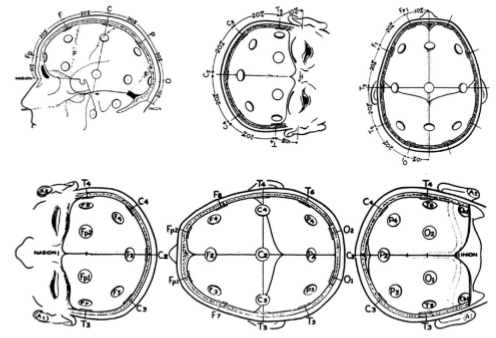
\includegraphics[width=0.8\linewidth]{figura_6.png} 
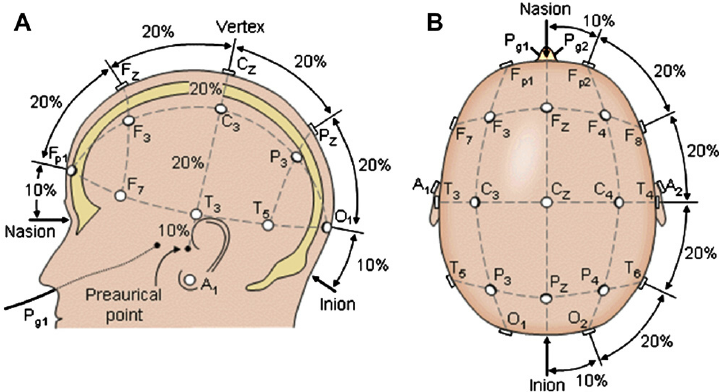
\includegraphics[width=0.9\linewidth]{Fig.png} 
\caption{El sistema 10--20, recomendado por la
International Federation of EEG Societies. [Este gr\'afico se volver\'a a dibujar]
%\cite{Jasper58,AASM07}
}
\label{img1020}
\end{figure}

Usualmente el EEG muestra una actividad el\'ectrica oscilatoria continua y cambiante. 
%Tanto la intensidad como los patrones de esta actividad est\'an determinados por los eventos de 
%excitaci\'on conjunta del cerebro, resultante de las funciones en el sistema reticular de 
%activaci\'on del tallo cerebral \cite{Clark98}.
Estas 'ondas' observadas en los registros de potenciales el\'ectricos en el cerebro son referidas 
como \textbf{ondas cerebrales}; la 'frecuencia' de estas ondas var\'ia entre 0.5 y 100 Hz, y se ha 
identificado que su composici\'on est\'a fuertemente relacionada con el grado de actividad cerebral: 
hay diferencias claras entre registros durante vigilia y sue\~no.
En general la frecuencia promedio del EEG incrementa progresivamente cuando hay un altos grados 
de actividad cerebral: las ondas se vuelven m\'as as\'incronas, de modo que la magnitud del 
potencial integrado de superficie decrece a pesar de la alta actividad cortical.
%Por ejemplo, las ondas delta se encuentran frecuentemente durante el estupor, anestesia 
%quir\'urgica, y sue\~no; las ondas theta son comunes en infantes; las ondas alfa ocurren en 
%estado de relajaci\'on; las ondas beta aparecen durante actividad mental intensa.
Aunque la mayor parte del tiempo el EEG es irregular y no muestra patrones claros, es com\'un que 
muestre ondas cerebrales relativamente organizadas que, para su estudio, han sido clasificadas en 
cuatro grandes grupos: alfa, beta, gamma, delta.
Estos grupos son ilustrados en la figura \ref{ritmos}.

\begin{figure}
\centering
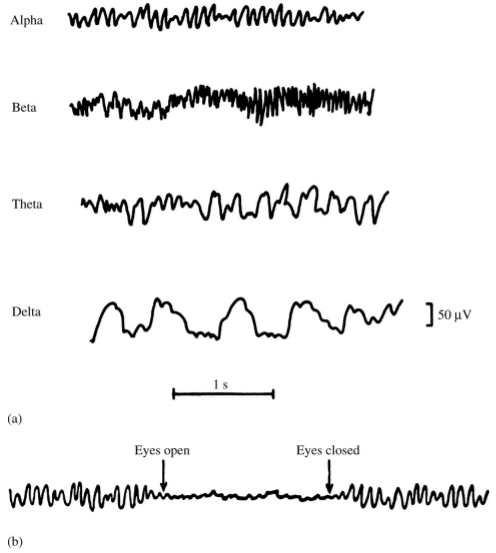
\includegraphics[width=0.5\linewidth]{figura_4.png} 
\caption{(a) Diferentes tipos de ondas normales en el EEG. (b) Supresi\'on del ritmo alfa debido a 
una descarga desincronizada cuando el paciente abre los ojos.
%(From A. C. Guyton, Structure and Function of the Nervous System, 2nd ed.,
%Philadelphia: W.B. Saunders, 1972; used with permission.)
[Estos gr\'aficos ser\'an reconstruidos]
}
\label{ritmos}
\end{figure}

\begin{description}
\item[Ondas alfa.] Frecuencias entre 8 y 13 Hz. Ocurren en sujetos despiertos en un estado de 
quietud del pensamiento. Aparecen m\'as frecuentemente en la regi\'on occipital, pero tambi\'en 
pueden ser registradas en las regiones frontal y parietal. Su voltaje aproximado est\'a entre 20 y 
200 mV. Cuando el sujeto duerme, las ondas alfa desaparecen completamente. Si el sujeto est\'a
despierto y su atenci\'on se dirige a una actividad mental espec\'ifica, las ondas alfa
son reemplazadas por ondas dessincronizadas de mayor frecuencia y menor voltaje.

\item[Ondas beta.] Frecuencias de 14 a 30 Hz. Normalmente se registran en las regiones parietal y 
frontal. A veces se les divide en dos tipos: beta I y beta II. Las ondas beta I (14--20 Hz)
son afectadas por la actividad mental de manera similar a las ondas alfa.
Las ondas beta II (20--30 Hz), en cambio, aparecen durante una activaci\'on intensa del sistema 
nervioso central y durante tensi\'on.

\item[Ondas theta.] Frecuencias entre 4 y 7 Hz. Ocurren principalmente en las regiones parietal y 
temporal en ni\~nos, pero pueden aparecer en algunos adultos durante estr\'es emocional, sobre 
todo durante periodos de decepsi\'on y frustraci\'on.

\item[Ondas delta.] Incluye todas las ondas del EEG 'abajo de' 3.5 Hz. Ocurren generalmente en el 
sue\~no profundo en infantes, y despu\'es de enfermedades org\'anicas serias del cerebro.
\end{description}
%Tambi\'en pueden ser registradas en cerebros de animales a los cuales se ha hecho transsecci\'on 
%subcortical, produciendo una separaci\'on funcional entre la corteza cerebral y el sistema 
%reticular de activaci\'on del tallo cerebral. 


Cabe mencionar que el espectro de frecuencias del potencial de campo producido por m\'usculos 
faciales medianamente contra\'idos, incluye componentes de frecuencia que bien cuadran en el rango 
usual del EEG (0.5--100 Hz).
%Una vez se ha conseguido el estado de reposo en un adulto normal, sus registros del cuero cabelludo
%muestran un ritmo alfa (ver m\'as adelante) dominante en el \'area parietal-occipital, mientras que 
%en \'area frontal ha un ritmo beta con baja amplitud y alta frecuencia --adem\'as del ritmo alfa.
%En un sujeto normal hay cierta simetr\'ia entre los registros de los hemisferios derecho e 
%izquierdo. 
La variedad de artefactos conocidos es muy basta, y constituye un tema muy complejo.

\subsection{Sue\~no}

Conviene presentar una definicici\'on formal de lo que es el sue\~no.
% y las etapas en que se
%divide para fines cl\'inicos --en particular, se manejan las caracter\'isticas recomendadas por 
%la AAMS \cite{AASM07}.
El sue\~no normal se divide en dos etapas principales: MOR (fase R) y NMOR (fase N), que se 
diferenc\'ian por sus rasgos electroencefalogr\'aficos y una serie de caracter\'isticas 
fisiol\'ogicas (de los cuales obtienen sus nombres).
Cabe mencionar que la nomenclatura acerca de las fases del sue\~no ha sido recientemente modificada 
por la American Association of Sleep Medicine en 2007 \cite{AASM07}, de modo que en este trabajo 
se usar\'an ambas nomenclaturas siempre que sea posible, por fines de compatibilidad.

\begin{description}
\item[Sue\~no] Proceso vital c\'iclico complejo y activo, compuesto por varias fases y que posee 
una estructura interna caracter\'istica, con diversas interrelaciones en los sistemas hormonales y 
nerviosos \cite{FernandezConde07}.
El sue\~no en el ser humano se puede caracterizar por las siguientes propiedades\cite{CarrilloMora}:
\begin{enumerate}
\item Disminuci\'on de conciencia y reactividad a est\'imulos externos
\item F\'acilmente reversible (lo cual lo diferencia de otros estados 
patol\'ogicos como el estupor y el coma)
\item Inmovilidad y relajaci\'on muscular
\item Periodicidad t\'ipica circadiana (diaria)
\item Los individuos adquieren una postura estereotipada
\item La privaci\'on induce alteraciones conductuales y 
fisiol\'ogicas, adem\'as de que genera una ''deuda'' acumulativa
\end{enumerate}
\end{description}


Durante el sue\~no MOR (fase R), ocurre que
las ondas lentas y amplitud alta son reemplazadas por ondas r\'apidas 
de bajo voltaje, irregulares, y que recuerdan la actividad en el EEG durante el estado de alerta.
La presencia de estos patrones irregulares no interrumpen el sue\~no, sino que incrementan el 
umbral para los est\'imulos externos; 
este comportamiento es referido como 'sue\~no parad\'ojico'.
Durante esta etapa de sue\~no, el sujeto exhibe movimientos oculares r\'apidos (MOR), raz\'on por 
la 
cual esta etapa recibe su nombre caracter\'istico.
%La etapa fuera del sue\~no
%es referida como sue\~no no-MOR (NMOR) o sue\~no de ondas lentas.
%Los sujetos humanos que despiertan durante la fase de sue\~no MOR suelen reportar que
%ten\'ian enso\~naciones, a diferencia de aquellos que despiertan durante la fase NREM.
Durante el sue\~no MOR se producen la mayor\'ia de las enso\~naciones (lo que conocemos 
coloquialmente como sue\~nos), y la mayor\'ia de los pacientes que despiertan durante esta fase 
suelen recordar v\'ividamente el contenido de sus enso\~naciones \cite{Chokroverty09}.
F\'isicamente el tono de todos los m\'usculos disminuye (con excepción de los m\'usculos 
respiratorios y los esf\'interes vesical 
y anal), as\'i mismo la frecuencia cardiaca y respiratoria se vuelve irregular.%,

El sue\~no fuera de la etapa MOR es referido como no-MOR (NMOR, fase N), y es dividido en 
etapas seg\'un la 'profundidad' del sue\~no --entendida en t\'erminos de la actividad cerebral registrada.
En el sue\~no profundo se observan ondas delta muy irregulares, y junto con ellas ocurren trenes 
cortos de ondas, parecidas a las alfa, y que son referidas como \textit{husos de sue\~no}. 
El ritmo alfa y los husos de sue\~no est\'an sincronizados en el sue\~no y la somnolencia 
--en contraste con la actividad irregular, desincronizada y de bajo voltaje registrada en estado de 
alerta.


%\begin{figure}
%\centering
%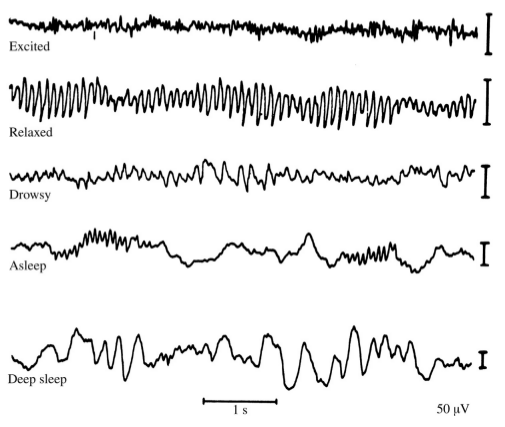
\includegraphics[width=0.5\linewidth]{figura_7.png} 
%\caption{Los cambios en el EEG que ocurren durante el sue\~no en un sujeto.
%Las marcas de calibraci\'on corresponden a 50 mV.
%%H. Jasper, ‘‘Electrocephalography.’’ In Epilepsy and Cerebral Localization, W.
%%G. Penfield and T. C. Erickson (eds.). Springfield, IL: Charles C. Thomas,
%%1941.)
%[Estos gr\'aficos ser\'an redibujados]
%}
%\label{ritmosEEG}
%\end{figure}



%El sue\~no MOR se caracteriza por la presencia de ondas de bajo voltaje y alta frecuencia en el 
%EEG, aton\'ia muscular y movimientos oculares r\'apidos, adem\'as es donde se presentan 
%la mayor\'ia de los sue\~nos. 
%El sue\~no no-MOR se compone de cuatro fases, 1 y 2, que son de sue\~no ligero, y 3 y 4 de 
%sue\~no profundo, las mismas que transcurren de manera secuencial desde la primera hasta la 
%cuarta fase, que es la fase reparadora del sue\~no, aquella que produce en la persona la 
%sensaci\'on de haber descansado cuando se levanta 13,22,43.

%Las características de las fases del sueño no-MOR incluyen cuatro etapas, la primera que 
%corresponde a la transición de la vigilia al sueño; la etapa 2 es la intermedia (mayor porcentaje 
%del tiempo de sueño) y en el EEG aparecen husos de sueño y los complejos K. La etapa 3 es la del 
%sueño relativamente profundo, representado en el electroencefalograma por ondas lentas de gran 
%amplitud, y la etapa 4o de sueño profundo con más del 50\% de ondas lentas de gran amplitud13.

%%%%%%%%%%%%%%%%%%%%%%%%%%%%%%%%%%%%%%%%%%%%%%%%%%%%%%%%%%%%%%%%%%%%%%%%%%%%%%%%%%%%%%%%%%%%%%%%%%%

%\begin{description}

\begin{description}
\item[Fase 1 (N1)] Corresponde con la somnolencia o el inicio del sue\~no ligero, en ella es muy 
f\'acil despertarse. La actividad muscular disminuye paulatinamente y pueden observarse algunas 
breves sacudidas musculares s\'ubitas que a veces coinciden con una sensación de ca\'ida 
(mioclon\'ias h\'ipnicas). En el EEG se observa actividad de frecuencias mezcladas, pero de bajo 
voltaje y algunas ondas agudas. 

\item[Fase 2 (N2)] Se caracteriza por que aparecen patrones espec\'ificos de actividad 
cerebral (husos de sue\~no y complejos K). La temperatura, la frecuencia card\'iaca y respiratoria 
comienzan a disminuir paulatinamente. 

\item[Fases 3 y 4 (N3)] La fase m\'as profunda del sue\~no NMOR. Se observan ondas con frecuencias 
muy bajas ($<2$ Hz), por lo que es referido como 'sue\~no de ondas lentas'.
\end{description}
%\item[Sueño MOR (fase R)] Se caracteriza por la presencia de movimientos oculares r\'apidos. F\'isicamente el tono de todos 
%los m\'usculos disminuye (con excepción de los m\'usculos respiratorios y los esf\'interes vesical 
%y anal), as\'i mismo la frecuencia cardiaca y respiratoria se vuelve irregular.%,
%%e incluso puede 
%%incrementarse y 
%%existe erección espontánea del pene o del clítoris. 
%%Durante el sue\~no MOR se producen la mayor\'ia de las enso\~naciones (lo que conocemos 
%%coloquialmente como sue\~nos), y la mayor\'ia de los pacientes que despiertan durante esta fase 
%%suelen recordar v\'ividamente el contenido de sus enso\~naciones \cite{Chokroverty09}.
%\end{description}

Un adulto j\'oven pasa aproximadamente entre 70--100 minutos en el sue\~no NMOR para despu\'es 
entrar al sue\~no MOR, el cual puede durar entre 5--30 min; este ciclo se repite cada hora y media.
%A lo largo de la noche pueden presentarse normalmente entre 4 y 6 ciclos de sue\~no MOR.
En los ancianos se va fragmentando el sue\~no nocturno con frecuentes episodios de despertar, se 
reduce mucho el porcentaje de sue\~no en fase 4, pero se mantiene constante el porcentaje de 
sue\~no MOR. Adicionalmente, muchos adultos mayores dormitan durante el d\'ia varias siestas 
cortas \cite{CarrilloMora}.

%
%Los adultos mayores informan que duermen menos durante la noche, y se acuestan y se despiertan 
%m\'as temprano de lo habitual. Adem\'as, tardan m\'as tiempo en conciliar el sue\~no, se 
%despiertan con m\'as frecuencia durante la noche y la duraci\'on de estos despertares es 
%m\'as prolongada 58,59.
%

%%%%%%%%%%%%%%%%%%%%%%%%%%%%%%%%%%%%%%%%%%%%%%%%%%%%%%%%%%%%%%%%%%%%%%%%%%%%%%%%%%%%%%%%%%%%%%%%%%%
%%%%%%%%%%%%%%%%%%%%%%%%%%%%%%%%%%%%%%%%%%%%%%%%%%%%%%%%%%%%%%%%%%%%%%%%%%%%%%%%%%%%%%%%%%%%%%%%%%%
%%%%%%%%%%%%%%%%%%%%%%%%%%%%%%%%%%%%%%%%%%%%%%%%%%%%%%%%%%%%%%%%%%%%%%%%%%%%%%%%%%%%%%%%%%%%%%%%%%%
%%%%%%%%%%%%%%%%%%%%%%%%%%%%%%%%%%%%%%%%%%%%%%%%%%%%%%%%%%%%%%%%%%%%%%%%%%%%%%%%%%%%%%%%%%%%%%%%%%%

%%%%%%%%%%%%%%%%%%%%%%%%%%%%%%%%%%%%%%%%%%%%%%%%%%%%%%%%%%%%%%%%%%%%%%%%%%%%%%%%%%%%%%%%%%%%%%%%%%%%
%%%%%%%%%%%%%%%%%%%%%%%%%%%%%%%%%%%%%%%%%%%%%%%%%%%%%%%%%%%%%%%%%%%%%%%%%%%%%%%%%%%%%%%%%%%%%%%%%%%

\section{Conceptos, matem\'aticas}

En esta secci\'on se describen los conceptos b\'asicos de la teor\'ia espectral 'cl\'asica' para 
procesos estacionarios, y la generalizaci\'on hecha por Priestley para procesos no-estacionarios. 
De forma m\'as bien pragm\'atica, la descripci\'on est\'a
 fuertemente inspirada por el libro 'Spectral Analysis and Time Series' 
de M. B. Priestley \cite{Priestley81}, ya que este est\'a expl\'icitamente dirigido a un p\'ublico 
sin un trasfondo matem\'atico.

Se suponen conocidos varios temas b\'asicos de probabilidad y estad\'istica:
variables aleatorias, valores esperados y momentos, estimadores y sus propiedades.
Con el fin de presentar la notaci\'on usada, se incluyen algunos conceptos previos a la 
definici\'on per se de estacionariedad y estimadores en el dominio de frecuencias.
%Chatfield (The Analysis of Time Series: An Introduction, 2003)

%%%%%%%%%%%%%%%%%%%%%%%%%%%%%%%%%%%%%%%%%%%%%%%%%%%%%%%%%%%%%%%%%%%%%%%%%%%%%%%%%%%%%%%%%%%%%%%%%%%

\subsection{Estacionariedad d\'ebil}

Para hablar formalmente de procesos estoc\'asticos como modelos, antes 
conviene escribir su definici\'on desde el punto de vista matem\'atico. Las siguientes definiciones
son aplicables tanto para procesos en tiempo continuo
como para procesos a tiempo discreto; aunque el objeto de estudio, el EEG, se considera 
un fen\'omeno continuo, s\'olo es posible registrarlo durante un conjunto finito de puntos 
en el tiempo.

\begin{defn}[Proceso estoc\'astico]
Un proceso estoc\'astico $\{ X(t) \}$ es una familia de variables aleatorias 
en los reales,
indexadas por
$t \in T \subseteq \R$.
%, mientras que una observaci\'on
%de $\{X(t)\}$ ser\'a denotada por $(x_1,x_2,\dots)$
\end{defn}

Como notaci\'on, una realizaci\'on de $X(t)$ ser\'a denota por $x_t$. 
Las funciones de densidad de probabilidad y de probabilidad acumulada para $X(t)$ ser\'an
referidas, respectivamente, como $f_{X(t)}$ y $F_{X(t)}$
%Cabe destacar que en esta definici\'on se omiti\'o intencionalmente pedir que las variables
%aleatorias sea reales, ya que eventualmente se considerar\'an procesos en los complejos.
Cabe enfatizar que para cada valor de $t$,
%tiempo $t$, 
$X(t)$ es una variable aleatoria; no se presupone ninguna conexi\'on entre ellas.
%con su funci\'on de densidad de probabilidad,
%sus momentos [s\'olo se consideran va's con al menos segundos momentos finitos], etc.


La caracter\'istica principal 
investigada en este trabajo hace referencia a la ''estacionariedad''. De manera 
informal, esta propiedad se refiere a que las variables aleatorias que conforman un proceso
estoc\'astico sean b\'asicamente iguales --dicho con otras palabras, que las propiedades
del proceso sean invariantes en el tiempo. 
Una definici\'on que satisface fielmente est\'a descripci\'on es la de estacionariedad 
en el sentido fuerte o estricto.
El t\'ermino ''tiempos admisibles'' simplemente indica que la definici\'on es la misma para
procesos a tiempo discreto o continuo, bajo restricciones obvias.

\begin{defn}[Estacionariedad fuerte]
Un proceso estoc\'astico $\{ X(t) \}$ es fuertemente estacionario si, para cualquier 
conjunto de tiempos admisibles $t_1,t_2,\dots,t_n$ y cualquier $\tau$ tal que 
 $t_i+\tau$ son tiempos admisibles para $i = 1, 2, \dots n$;
se cumple que
\begin{equation*}
F_{\left(X(t_1),X(t_2),\dots,X(t_n)\right) }
\equiv
F_{\left(X(t_1+\tau),X(t_2+\tau),\dots,X(t_n+\tau)\right)}
\end{equation*}

Donde $F_{\left(X(t_1),X(t_2),\dots,X(t_n)\right) }$ es la funci\'on de distribuci\'on de
probabilidad conjunta del vector $\left(X(t_1),X(t_2),\dots,X(t_n)\right)$
\end{defn}

Esta definici\'on, sin embargo, no resulta muy \'util en el contexto de la estad\'istica:
si se supone que el registro de un fen\'omeno puede interpretarse como \textbf{una} 
realizaci\'on de
un proceso estoc\'astico, entonces para cada tiempo se tiene una \'unica observaci\'on
de cada variable aleatoria. A esto hay que a\~nadir que, para un fen\'omeno continuo,
no todas los tiempos son registrables.
Luego, si no existe la garant\'ia de que las propiedades de estas variables aletorias sean
''similares'', entonces es virtualmente imposible obtener mayor informaci\'on de ellas.

Es bajo estas limitaciones que se motiva un concepto de estacionariedad m\'as d\'ebil, pero que
satisfaga ''suficientes teoremas importantes'' y que sea relevante bajo las restricciones
propias de diferentes campos. En este trabajo se ha optado por la llamada 
''estacionariedad d\'ebil'' o estacionariedad de orden 2, que recibe su nombre como caso
particular de la ''estacionariedad de orden $m$''.

\begin{defn}[Estacionariedad de orden $m$]
Un proceso estoc\'astico $\{ X(t) \}$
se dice estacionario de orden $m$ si, para cualquier 
conjunto de tiempos admisibles $t_1,t_2,\dots,t_n$ y cualquier $\tau \in \R$
se cumple que
\begin{equation*}
\E{ X^{m_1}(t_1)X^{m_2}(t_2)\cdots X^{m_n}(t_n) }
=
\E{ X^{m_1}(t_1+\tau)X^{m_2}(t_2+\tau)\cdots X^{m_n}(t_n+\tau) }
\end{equation*}
Para cualesquiera enteros $m_1,m_2,\dots,m_n$ tales que $m_1+m_2+\dots+m_n \leq m$
\label{est_orden_m}
\end{defn}

La estacionariedad d\'ebil no pide que la funci\'on
de distribuci\'on conjunta tenga determinada forma, sino que los momentos conjuntos sean 
invariantes ante traslaciones en el tiempo. Para entender mejor esta diferencia, consid\'erense
tres procesos $\{X(t)\}$, $\{Y_1(t)\}$ y $\{Y_2(t)\}$, de modo que el primero es
estacionario en el sentido fuerte, el segundo es estacionario de orden 1 y el tercero es
estacionario de orden 2.
\begin{itemize}
\item Por definici\'on $F_{X(t) } \equiv F_{X(t+\tau)}$ para cualesquieras $t$, $t+\tau$
admisibles; entonces $\E{X(t)} = \mu_X$ es constante
\item Por definici\'on
para cualesquieras $t$, $t+\tau$ admisibles se tiene que $\E{Y_1(t)}=\E{Y_1(t+\tau)}$ y
$\E{Y_2(t)}=\E{Y_2(t+\tau)}$. Se deduce que $\E{Y_1(t)} = \mu_{Y_1}$, 
$\E{Y_2(t)} = \mu_{Y_2}$ son constantes
\item Usando nuevamente que $F_{X(t) } \equiv F_{X(t+\tau)}$ para cualesquieras $t$, $t+\tau$
admisibles, se deduce que $\Var{X(t)} = \sigma_X$ es constante
\item Por definici\'on de $\mathrm{Var}$ y de $Y_i$ ($i=2,1$)
$$\Var{Y_i(t)} = \E{Y_i^{2}(t)} - \left( \E{Y_i(t)} \right)^{2} = \E{Y_i^{2}(t)} - \mu_{Y_i}$$
Luego se puede deducir que 
$\Var{Y_2(t)}$ es
% $\E{Y_2^{2}(t)}$ es
constante, mientras que no se puede garantizar lo mismo para $\Var{Y_1(t)}$
% Se concluye que la varianza
%de $Y_2$ es constante en el tiempo mientras que la de $Y_1$ no necesariamente lo es
\item El \textit{coeficiente de asimetr\'ia de Fisher} 
de una variable aleatoria $V$ se define como
$$
\gamma_1(V) = \frac{\E{\left(V-\E{V}\right)^{3}}}{\Var{V}^{\nicefrac{3}{2}}}
$$
%= \frac{\E{X^{3}}-3\mu_V \E{V^{2}}+2\mu_V^{3}}{\Var{V}^{\nicefrac{3}{2}}}
%$$
Sin entrar en detalles, se puede deducir que $\gamma_1(X(t))$ es constante mientras que no se
puede garantizar lo mismo para $\gamma_1(Y_1(t))$, $\gamma_1(Y_2(t))$
\end{itemize}

Naturalmente hay una relaci\'on de contenci\'on clara en
la familia de los conjuntos de procesos estacionarios de orden finito:
si un proceso es estacionario de orden $m$, entonces es estacionario de orden $n$ para todo
$n \leq m$. Es posible incluso describir procesos que sean estacionarios de orden ''infinito''
y preguntarse bajo qu\'e condiciones son fuertemente estacionarios.
Tal discusi\'on no se incluye en el presente trabajo.
%,
%% con el fin de ser concreto.
%ya que 
%%el enfoque es de modelaci\'on y 
%se ha intentado hacer la menor cantidad posible de supuestos y de proporcionara a cada uno una
%''interpretaci\'on fisiol\'ogica''.


%As\'i pues, y dadas 
Una vez hechas
las consideraciones anteriores, conviente
introducir una segunda caracter\'izaci\'on de los procesos estacionarios de orden 2 --d\'ebilmente 
estacionarios--
% enlistar las siguientes propiedades para un proceso
%estacionario de orden 2 --o d\'ebilmente estacionario-- 
que es equivalente
%\footnote{Este hecho se vuelve claro si se analizan cuidadosamente las propiedades
%enlistadas y se comparan con las deficiniones de las ''cantidades'' involucradas}
a la definici\'on \ref{est_orden_m} pero cuya interpretaci\'on suele considerarse como m\'as clara
%Hay una especie de consenso seg\'un el cual la estacionariedad de orden 2, tambi\'en
%llamada \textbf{estacionariedad d\'ebil} es suficiente para
%que se cumplan los teoremas m\'as comunes sobre medias y varianzas.
%Algunas consecuencias que un
%proceso sea estacionario debilmente son las siguientes:
\begin{thrm}
Un proceso es d\'ebilmente estacionario si y s\'olo si para cualesquiera tiempos admisibles
$t$, $s$ se tiene que
\begin{itemize}
\item $\E{X(t)} = \mu_X$
\item $\Var{X(t)} = \sigma^{2}_X$
\item $\Cov{X(t),X(s)} = \rho (s-t)$
\end{itemize}
Donde $\mu_X$, $\sigma^{2}_X$ son constantes, $\rho(\tau)$
es una funci\'on que \'unicamente depende de $\tau$
\label{est_usual}
\end{thrm}

A grosso modo, cuando uno se refiere a un proceso d\'ebilmente estacionario seg\'un
\ref{est_orden_m} se le pide que su primer y segundo momentos sean constantes, as\'i como
el primer momento conjunto s\'olo dependa del lag en el tiempo. A su vez, seg\'un 
\ref{est_usual} un proceso es d\'ebilmente estacionario si su media y varianza son constantes en
el tiempo, y su funci\'on de autocovarianza s\'olo depende del lag en el tiempo.

Cabe mencionar, como comentario, que es posible contruir procesos que sean fuertemente
estacionarios pero que no sean estacionarios de ning\'un orden finito; dado que
la primera definici\'on se basa en funciones de densidad de probabilidad mientras que la segunda
se basa en momentos, es suficiente con usar variables aleatorias que no tengan todos
sus momentos bien definidos. Por ejemplo, consid\'erese un proceso conformado por variables
aleatorias independientes id\'enticamente distribuidas con distribuci\'on de Cauchy.

Dado que en el EEG se miden fluctuaciones en potenciales de campos el\'ectricos
%(medida en mV),
que (en este trabajo) se modelan como variables aleatorias, 
la intepretaci\'on usual para los momentos de estas variables est\'a ligado a la distribuci\'on de
energ\'ia asociada al sistema. Luego, es plausible considerar que el EEG es un fen\'omeno
''suficientemente regular'' como para que las variables aleatorias del modelo tengan cuando
menos segundos momentos bien definidos.

%%%%%%%%%%%%%%%%%%%%%%%%%%%%%%%%%%%%%%%%%%%%%%%%%%%%%%%%%%%%%%%%%%%%%%%%%%%%%%%%%%%%%%%%%%%%%%%%%%%

\subsection{Espectro de un proceso estacionario}

Existe una larga tradici\'on en las ciencias biom\'edicas para interpretar a los registros
electrofisiol\'ogicos en t\'erminos de ondas y frecuencias, ya que fundamentalmente se
trata de fen\'omenos el\'ectricos \cite{Kaiser00}. 
As\'imismo existe una teor\'ia matem\'atica bien desarrollada sobre estad\'istica en el 
llamado ''dominio de las frecuencias''. 
En este trabajo se aborda la segunda como forma de tener coherencia con la primera; a continuaci\'on
se describen los conceptos m\'as importantes en el modelo usado.

Un objeto fundamental para el estudio del dominio de las frecuencias\footnote{Este concepto 
no se
%discutir\'a en el presente trabajo, sino que 
ser\'a manejado pragm\'aticamente para referirse
al cambio de coordenadas inducido por la transformada de Fourier o alguna generalizaci\'on de la 
misma} son las series de Fourier y sus generalizaciones. 

\begin{defn}[Serie de Fourier]
Sea $f$ una funci\'on peri\'odica con periodo $2\pi$ tal que $\intR \abso{f(t)} dt < \infty$. 
Si se calculan los coeficientes
\begin{equation*}
A_n = \frac{1}{2\pi} \intPI f(t) e^{- i n t} dt
\end{equation*}
entonces la siguiente igualdad se cumple casi en todas partes
\begin{equation*}
f(x) = \sum_{n=-\infty}^{\infty} A_n e^{i n t}
\end{equation*}
La sucesi\'on $\left( A_n \right)$ ser\'a referida como \textbf{serie de Fourier} de la funci\'on
$f$.
\label{FourierClasico}
\end{defn}

%\begin{defn}[Transformada de Fourier (funciones peri\'odicas)]
%Sea $f$ una funci\'on peri\'odica con periodo $2\pi$ tal que $\intR \abso{f(t)} dt < \infty$.
%hjkjkjkj
%\end{defn}

Por el momento no se discutir\'an los detalles sobre la convergencia de las sucesiones de 
\ref{FourierClasico}, siempre que se limite a funciones 
peri\'odicas,
continuas y absolutamente sumables,
%$L^{1}\left([-\pi,\pi])\right)$
o se permita que sean acotadas y con
una cantidad finita de discontinuidades --y se ponga ninguna atenci\'on sobre ellas.
Parece claro que se puede definir una funci\'on --quiz\'a invertible-- que mapee funciones 
a sus respectivas series de Fourier;
%que
%poseen serie de Fourier a ''alg\'un'' conjunto de series absolutamente sumables $\ell$; 
esta
funci\'on es referida como \textbf{transformada de Fourier}. Por lo pronto se considerar\'a
que las propiedades y limitaciones de la transformada de Fourier son conocidas
al menos a grosso modo, m\'as que nada por brevedad; se pretende exhibir
el espectro de potencias para una serie de tiempo como una extensi\'on de la
transformada de Fourier de modo que se espera
poder enfatizar sobre algunas
interpretaciones dentro de la modelaci\'on.
%conocidas y demostradas todas sus propiedades.

%%%%%%%%%%%%%%%%%%%%%%%%%%%%%%%%%%%%%

\subsubsection{Notas sobre interpretaci\'on f\'isica}

Las series de Fourier gozan de una interpretación física muy extendida como que una 
se\~nal\footnote{Esta palabra se usar\'a para referirse a un fen\'omeno f\'isisco 
que est\'a siendo 
registrado, bajo el entendido que es casi lo mismo referirse al registro o al proceso
que lo genera si \'este es determinista}
peri\'odica
puede verse como la superposici\'on de se\~nales peri\'odicas m\'as simples. 
De igual forma es destacable su interpretaci\'on como ''coordenadas'' en un espacio de funciones
dada una base ortonormal del mismo. 
El estudio de estos espacios dentro del an\'alisis trae a la mente
la cuesti\'on de convergencia,
el problema del subespacio de
funciones medibles de medida cero, y la posibilidad de otras bases; estos fen\'omenos tienen a su 
vez una interpretaci\'on f\'isica como cambios s\'ubitos en la energ\'ia, el ruido y la 
tipificaci\'on de ondas ''simples'' --por ejemplo, las ondas cuadradas y triangulares son 
m\'as comunes en teor\'ia de circuitos.

Para limar estas ambig\"uedades, en este trabajo se considerar\'a la base de Fourier como la
''m\'as natural'' por su conexi\'on simple con las exponenciales complejas. El t\'ermino
''ruido'' ser\'a evitado en la medida de lo posible ya que, en la terminolog\'ia de se\~nales,
suele referirse a registros con un comportamiento err\'atico y poco
predecible; dentro del contexto de electrofisiolog\'ia, tal descricpi\'on bien
puede englobar tanto
se\~nales que
se desea estudiar, como interferencias y errores.
%Para los procesos estoc\'asticos que son considerados en este trabajo, 
Conviene definir
un tipo de ''regularidad estoc\'astica'' que sirva para distinguir los patrones buscados
de errores de medici\'on e interferencias.

\begin{defn}[Continuidad estoc\'astica (media cuadr\'atica)]
Un proceso estoc\'astico a tiempo continuo $\{ X(t) \}$ es estoc\'asticamente continuo
(en el sentido de media cuadr\'atica)
en un tiempo admisible $t_0$ si y s\'olo si
\begin{equation*}
\lim_{t \rightarrow t_0} \E{\left( X(t) - X(t_0) \right)^{2}} = 0
\end{equation*}
\label{cont_est}
\end{defn}

Una forma natural de pensar en la definici\'on \ref{cont_est} es esperar que en promedio
$\lim_{t \rightarrow t_0} \left( X(t) - X(t_0) \right)^{2} = 0$. 
No es la \'unica forma de presentar un l\'imite de variables aletorias, sino que se ha elegido
esta forma por algunas propiedades que ser\'an explotadas m\'as adelante. 
As\'imismo cabe destacar que un proceso estoc\'asticamente continuo no necesariamente produce 
realizaciones que son funciones continuas, sino que sus realizaciones deben ser continuas 
casi en todas partes\footnote{Una funci\'on es \textit{continua casi en todas partes} si
es continua en todo su dominio excepto por un conjunto de medida cero}.

El arquetipo de esta clase de procesos es el proceso de Wiener.
%
%Por ejemplo, un proceso de Poisson es estoc\'asticamente continuo aunque sus realizaciones
%nunca son continuas; un proceso ruido blanco (variables aleatorias indepentiendes
%e id\'enticamente distribuidas)
%no es estoc\'asticamente continuo ya que puede 
%
%Para explorar este concepto de manera concreta, consid\'erese un proceso de Wiener; como es 
%un ejemplo ''r\'apido'', se definir\'a a apartir de sus propiedades:
%
%\begin{defn}[Proceso de Wiener]
%Un proceso estoc\'astico a tiempo continuo $\{ W(t) \}$ recibe el nombre de proceso
%de Wiener si satisface que
%\begin{itemize}
%\item $W(0) = 0$
%\item La variable aleatoria $W(t) - W(s)$ tiene una distribuci\'on normal con media 0 y 
%varianza $\abso{t-s}$
%\item Las variables aleatorias ${W(t)}$ y ${W(t) - W(s)}$ son independientes para
%todos los tiempo permitidos $t$, $s$
%\end{itemize} 
%\end{defn}
%
%Ahora bien, se considera un proceso de Wiener $\{W(t)\}$ con $t\geq 0$, y se verificar\'a su 
%continuidad estoc\'astica para un punto arbitrario $t_0 > 0$. 
%Por definici\'on, se tiene
Para mostrarlo, consid\'erese un proceso de Wiener $\{W_t\}$; 
por su definici\'on se tiene que
$$W(t) - W(t_0) \sim N(0,\abso{t-t_0}) \sim \sqrt{\abso{t-t_0}} N(0,1)$$
donde el s\'imbolo $\sim$ indica que dos variables tienen la misma funci\'on de densidad de 
probabilidad. Luego, como $ \left( W(t) - W(t_0) \right)^{2} \sim \chi^{2}(1) $, se cumple que
$$
\E{\left( W(t) - W(t_0) \right)^{2}}
$$
y luego entonces es claro que $\lim_{t \rightarrow t_0} \E{\left( X(t) - X(t_0) \right)^{2}} = 0$.
Esta aritm\'etica de variables aleatorias puede formalizarse, pero a lo largo de
este trabajo se supondr\'an conocidos los detalles respectivos.

De manera m\'as general, cabe mencionar un teorema que permite tipificar de manera m\'as
adecuada esta clase de procesos.

\begin{thrm}
Un proceso d\'ebilmente estacionario a tiempo continuo es estoc\'asticamente continuo si y s\'olo si
su funci\'on de autocorrelaci\'on es continua en 0
\end{thrm}
\begin{demostracion}
Sea $\{ X(t) \}$ un proceso d\'ebilmente estacionario, y sea $t_0$ un tiempo admisible arbitrario. 
Luego, para todo $t$ admisible se cumple que
\begin{align*}
\E{\left( X(t) - X(t_0) \right)^{2}}
&= \Var{X(t)} + \Var{X(t_0)} - 2 \Cov{X(t)}{X(t_0)}
\\
&= 2 \sigma_X^{2} \left( 1 - \rho(t-t_0) \right)
\end{align*}
donde $\rho$ es la funci\'on de autocorrelaci\'on y $\sigma_X^{2}$ la varianza del proceso. 
Luego es claro que
\begin{align*}
\lim_{t\rightarrow t_0} \E{\left( X(t) - X(t_0) \right)^{2}} = 0  
&{\Leftrightarrow}
\lim_{t\rightarrow t_0} 2 \sigma_X^{2} \left( 1 - \rho(t-t_0) \right) = 0
\\
&{\Leftrightarrow}
\lim_{\tau \rightarrow 0} \rho(\tau) = 1
\end{align*}
Como siempre se cumple que $\rho(0)=1$, la condici\'on final se traduce en que $\rho$ sea continua 
en 0
\end{demostracion}

Con esta segunda caracterizaci\'on a la mano, es f\'acil afirmar que un proceso %donde todas
%conformado por variables aleatorias independientes 
ruido blanco
no es estoc\'asticamente continuo,
ya que su funci\'on de autocorrelaci\'on vale 0 en todos los puntos
excepto en 0, donde vale 1.

En este trabajo se supondr\'a que los registros de PSG corresponden a realizaciones
de procesos estoc\'asticamente continuos; se considera la posiblidad de que est\'en
''contaminados'' por ''ruidos'', entendidos como procesos independientes de los potenciales de 
campo 
en el cerebro, de amplitud negligible y que ''muy posiblmente'' son estoc\'asticamente discontinuos 
casi en todas partes.

%---------------------------------------------------------------------------------------------------

Con respecto al concepto de energ\'ia, en este trabajo se usar\'a 
%formalmente desde un resultado
%usual, que se tomar\'a como definici\'on: 
desde la interpretaci\'on usual de teor\'ia de circuitos, pero que formalmente fungir\'a 
como definici\'on:
la energ\'ia disipada por la se\~nal $f$ 
%en el intervalo
%de tiempo $(t_1,t_2)$
est\'a dada por la expresi\'on \ref{energia}; si se divide tal expresi\'on
por $T$ se obtiene la \textit{potencia} (energ\'ia por unidad de tiempo)

%\begin{definition}[Energ\'ia y potencia de una se\~nal]
%
%\end{definition}

\begin{equation}
\int_{-T}^{T} \abso{f\left(t\right)}^{2} dt
\label{energia}
\end{equation}

%En este contexto
Vale la pena mencionar que este concepto de energ\'ia, como 
integral
%aporte conjunto
de una forma cuadr\'atica, es com\'un a varias ramas de la f\'isica y se encuentra ampliamente
extendido en las ingenier\'ias; en la econom\'ia, en cambio, no hay una motivaci\'on clara para
hacer uso de este concepto. 
Las t\'ecnicas electrofisi\'ologicas, concebidas dentro de la teor\'ia de circuitos, hereda la
terminolog\'ia e interpretaci\'on de energ\'ia.
%de modo que en 
En
este trabajo no s\'olo se contempla
como ''muy natural'' la idea de energ\'ia en los campos el\'ectricos del cerebro, sino que se
supondr\'a que esta es acotada para cualquier intervalo finito.
%Despu\'es de todo, el an\'alisis espectral tiene sus orignes en la f\'sicia, 

Contemplando este panorama, conviene se\~nalar
una relaci\'on cl\'asica entre la energ\'ia de una se\~nal
peri\'odica y su serie de Fourier (teorema \ref{parseval_serie});
tal idea ser\'a de gran importancia posteriormente en este trabajo.  

\begin{defn}[Relaci\'on de Parseval (funciones peri\'odicas)]
Sea $f$ una funci\'on peri\'odica de periodo $2T$ tal que acepta una representaci\'on como serie
de Fourier
\begin{equation*}
f(x) = \sum_{n=-\infty}^{\infty} A_n e^{i n t}
\end{equation*}
con $A_n = \frac{1}{2\pi} \intPI f(t) e^{- i n t} dt$. Entonces se cumple que
\begin{equation*}
\int_T^{T} X^{2}(t) dt = \sum_{n=-\infty}^{\infty} \abso{A_n}
\end{equation*}
\label{parseval_serie}
\end{defn}

Aunque esta afirmaci\'on
es relativamente simple desde la \'optica del An\'alisis funcional, tiene una interpretaci\'on
f\'isica importante: si una se\~nal puede descomponerse como una transposici\'on (suma) de 
se\~nales ortogonales simples, entonces su energ\'ia debe ser la suma de las energ\'ias 
asociadas a cada una de estas se\~nales. M\'as a\'un, un cambio en alguna de las se\~nales
ortogonales (base) afecta a la cantidad total de energ\'ia --pero no a las otras se\~nales base.
Incluso,
la independencia de las se\~nales base sugiere que la energ\'ia puede ser tratada separadamente
para cada se\~nal base. Luego, el m\'odulo de la serie de Fourier indica de cierto modo
c\'omo se distribuye la energ\'ia (o potencia) sobre las se\~nales base; por esta raz\'on se le
suele referir como \textbf{espectro de potencia}\footnote{Dada esta discusi\'on, conviene 
distinguir el \textit{espectro de potencia no-normalizado} como la energ\'ia definida como
en \ref{energia} usando \ref{parseval_serie}, mientras que un \textit{espectro de potencia 
normalizado} se puede definir de la misma forma pero diviendo la expresi\'on en 
\ref{energia} por $2T$}.

%---------------------------------------------------------------------------------------------------

%En el contexto de series electrofisiol\'ogicas, se mencion\'o que en el EEG se han descrito y
%patrones llamados ''ondas de sue\~no'' \footnote{Para m\'as informaci\'on ver
%las secciones anteriores}. Hist\'oricamente estas ondas fueron tipificados mediante el 
%uso de registros electroencefalogr\'aficos en papel, de modo que se define emp\'iricamente
%la ''frecuencia'' de una onda se sue\~no al contar el n\'umero de altibajos en una unidad
%de tiempo \cite{Klonowski09}. En un plano muy formal, no se espera que una onda  de sue\~no
%tenga una transformada de Fourier, al menos en el sentido cl\'asico; por otro lado, se espera que
%pueda formalizarse el concepto de una onda ''parecida'' a unacua frecuencia es tal.

En este caso, se presentar\'a la transformada de Fourier-Stieltjes. En primera instancia
%permite frecuencias puntuales que son inconmensurables con respecto al intervalo $[-\pi,'pi]$,
%de modo que 
acepta funciones no-peri\'odicas pero que pueden ser representadas como suma de funciones
peri\'odicas, la diferencia m\'as notable es que permite involucar funciones cuya frecuencia
es inconmensurable con respecto al intervalo $[-\pi,\pi]$ como por ejemplo la funci\'on
$$
f(x) = \COS{x} + \COS{x\sqrt{2}}
$$
no tiene una serie de Fourier, pero puede ser representada como una integral de Fourier-Stieltjes.

%---------------------------------------------------------------------------------------------------

Dicho esto, conviene indagar sobre las propiedades de las
funciones involucradas en una
transformada de Fourier-Stieltjes: no-negativas, monotonamente crecientes; si se habla de funciones
con energ\'ia finita se puede tambi\'en asegurar que son acotadas.
%son similares a una 
La transformada de Fourier-Stieltjes es una medida en alg\'un espacio --el nombre daba
algunas pistas al respecto. 
%--el nombre da pistas al respecto.

Si bien, dentro de la interpretaci\'on f\'isica, parece muy
la caracterizaci\'on de la transformada de Fourier-Stieltjes como una medida en alg\'un espacio 
--que posiblemente est\'e asociado a la distribuci\'on de energ\'ia--, desde el punto de vista
formal tiene consecuencias bastante interesantes.
Por ejemplo, basta citar un corolario del teorema de separaci\'on de Lebesgue, seg\'un el cual
toda funci\'on 

\begin{thrm}[Descomposici\'on de Lebesgue --sobre la medida de Borel]
asdasdasdsa
\end{thrm}

sdfgdsgdsfgsdfgsdfgdsgsdfgsdf

%---------------------------------------------------------------------------------------------------

%%%%%%%%%%%%%%%%%%%%%%%%%%%%%%%%%%%%%

Una pregunta natural cuando se toma la terminolog\'ia de ondas y frecuencias dentro
del estudio de series de tiempo, es sobre el significado de aplicar la transformada de Fourier a
un proceso estoc\'atico --o cuando menos a alguna sus realizaciones.
¿Bajo qu\'e condiciones las realizaciones de un proceso estoc\'astico admiten una representaci\'on
como series/integrales de Fourier/Fourier-Stieltjes?

(Por simplicidad se abordar\'a primero esta pregunta para procesos a tiempo continuo, y 
posteriormente se tratar\'a el caso a tiempo disreto.)

Se sabe que una condici\'on suficiente para que exista la transformada de Fourier de una funci\'on
dada, es que pertenezca al espacio de las funciones $L^2$, definido como
\begin{equation*}
L^2(\R) = \left\{ f: \R \rightarrow \R {\biggr\rvert} \int_{-\infty}^{\infty} f(x) dx < \infty \right\}
\end{equation*}

Sin embargo, considerando un proceso estacionario $\{ X(t) \}$, y dado que tiene varianza constante 
en el tiempo, se 
espera que sus realizaciones $x(t)$ no decaigan en infinito. Por otro lado, tampoco hay garant\'ia
que admita una representaci\'on de Fourier-Stieltjes. M\'as a\'un, no hay garant\'ia alguna que
una realizaci\'on arbitraria pueda expresarse como la suma de una funci\'on en $L^2$ y una
funci\'on que admita representaci\'on de Fourier-Stieltjes.

El enfoque que se aborda es construir una sucesi\'on de funciones 
%peri\'odicas 
en $L^{2}$
que convergen a ''cada''
$x(t)$, y luego revisar la convergencia de sus respectivas integrales de Fourier.
As\'i entonces, para cada $T>0$ se define
\begin{equation}
x_T(t) = 
\begin{cases}
x(t) & \text{ , } -T\leq t \leq T
\\
0 & \text{ , otro caso}
\end{cases}
\end{equation}

Claramente, para todo $T$ se tiene que $x_T \in L^2$, y entonces admite la siguiente 
representaci\'on
\begin{equation}
x_T (t) = \frac{1}{\sqrt{2 \pi}} \intR G_T(\omega) e^{i \omega t} d\omega
\end{equation}

Donde se define la funci\'on $G_T$ como

\begin{equation}
G_T (\omega) = \frac{1}{\sqrt{2 \pi}} \intR x_T(t) e^{-i \omega t} dt
= \frac{1}{\sqrt{2 \pi}} \int_{-T}^{T} x(t) e^{-i \omega t} dt
\end{equation}

Como se mencion\'o anteriormente no hay garant\'ia de que $x(t)$, una realizaci\'on arbitraria de
$\{X(t)\}$, tenga una integral de Fourier bien definida. Luego entonces no hay garant\'ia que 
$G_T$ converja cuando $T\rightarrow \infty$. Recuperando la interpretaci\'on de 
$\left| G_T(\omega) \right|^{2}$ como una funci\'on de densidad para la energ\'ia total del sistema 
asociada a la frecuencia
puntual $\omega$, destaca un argumento f\'isico seg\'un el cual $G_T$ no tiene por qu\'e converger:
durante un tiempo infinito, un sistema que maneja ''niveles constantes'' de 
energ\'ia puede registrar una cantidad infinita de energ\'ia en su historial. 
%Curiosamente,
%esta segunda interpretaci\'on del
%problema motiva una soluci\'on para el mismo: usando un tipo de promedio para la
%distribuci\'on de energ\'ia involucrando a $T$
Este problema puede remediarse resolviendo el enredo de palabras y t\'erminos, 
ya que no es tan importante la
cantidad de energ\'ia concentrada en cada frecuencia, sino qu\'e frecuencias concentran m\'as
energ\'ia. Luego entonces conviene usar un promedio que ''tome en cuenta'' el tama\~no
del intervalo

\begin{equation}
\lim_{T\rightarrow{\infty}} = \frac{ \left| G_T(\omega) \right|^{2}}{2 T}
\label{yacasi}
\end{equation}

La expresi\'on en \ref{yacasi} es una adaptaci\'on de la integral de Fourier para una realizaci\'on
de un proceso estoc\'astico a tiempo continuo; los detalles sobre la convergencia de esta 
cantidad se discutir\'an m\'as adelante.
%conserva una parte clave de la interpretaci\'on.
Por mientras, en cierta medida se ha contestado una de las interrogantes al inicio de esta 
secci\'on sobre la posibilidad y
el posible significado de una transformada de Fourier para las realizaciones de un proceso 
estoc\'astico; con respecto a la posibilidad de una transformada para el proceso per se, vale la 
pena
ajustar la definici\'on en \ref{yacasi} para que sea ''representativa'' del proceso --y no s\'olo
de una realizaci\'on particular. Priestley introduce la siguiente funci\'on

\begin{equation}
h(\omega) = \lim_{T\rightarrow \infty} \E{ \frac{ \left| G_T(\omega) \right|^{2}}{2 T} }
\end{equation}

La funci\'on $h$ es referida como la \textit{funci\'on de densidad espectral no-normalizada} para
$\{X(t)\}$. Posteriormente se definir\'a una versi\'on ''normalizada'' de la SDF, pero antes debe
definirse la ''potencia total'' del proceso; por simplicidad, antes de ello se exhibir\'an
algunas propiedades de la SDF, adem\'as algunos teoremas importantes.

%%%%%%%%%%%%%%%%%%%%%%%%%%%%%%%%%%%%%%%%%%%%%%%%%%%%%%%%%%%%%%%%%%%%%%%%%%%%%%%%%%%%%%%%%%%%%%%%%%%

\subsection{Estimaci\'on de la SDF}

En la subsecci\'on anterior se exhibi\'o una forma de definir un espectro de potencias para 
procesos estoc\'asticos estacionarios --hasta ahora se ha supuesto que tienen cuando menos
segundos momentos finitos. Esta definici\'on es resumida en \ref{SDF} para el caso no-normalizado;
como el operador $\mathrm{E}$ indica el valor esperado sobre todas las realizaciones del proceso,
la definici\'on se hescribi\'o en t\'erminos del proceso y no de sus realizaciones.

\begin{defn}[Funci\'on de densidad espectral (SDF) no-normalizada]
Sea $\{X(t)\}$ un proceso estoc\'astico at iempo continuo, d\'ebilmente estacionario. Se define
la funci\'on de densidad espectral (SDF) de $\{X(t)\}$ como
%a tiempo continuo 
%tal que para todo tiempo admisible $t$ se cumple que $\E{X(t)}$
\begin{equation*}
h(\omega) = \lim_{T\rightarrow \infty} \E{ \frac{ \left| G_T(\omega) \right|^{2}}{2 T} }
\end{equation*}
Donde $G_T (\omega) = \frac{1}{\sqrt{2 \pi}} \int_{-T}^{T} X(t) e^{-i \omega t} dt$
\label{SDF}
\end{defn}

%Como se mencion\'o anteriormente, se omiti\'o intencionalmente una discusi\'on sobre el proceso hasta
%ahora. Y e

%Consid\'erese un ejemplo hip\'otetico de ondas cerebrales alfa de 10 Hz, donde el ruido externo 
%ha sido eliminado completamente; este registro te\'orico se 

La discuci\'on sobre la convergencia de $h$ se omiti\'o por tiempo y simpleza de la explicaci\'on,
aunque basta con intentar aplicar la definici\'on \ref{SDF} a una funci\'on determinista
continua y peri\'odica --puede interpretarse como un proceso estoc\'astico degenerado, 
con varianza 0
para cualquier tiempo permitido. 
Como toda funci\'on peri\'odica continua posee una serie de Fourier bien definida, la SDF del
proceso debe ''coincidir'' en cierto sentido. 
Desde la interpretaci\'on f\'isica, tiene sentido que la energ\'ia de una se\~nal peri\'odica
debe estar distribuida entre se\~nales peri\'odicas --caso contrario, sus ''modos'' ser\'ian
imcompatibles y perder\'ian energ\'ia al interactuar--; luego la distribuci\'on de energ\'ia
debe tener picos tipo ''delta de Dirac'' en las frecuencias compatibles.

Desde el punto de vista matem\'atico, m\'as interesante,
el conjunto de las funciones que tienen transformada de 
Fourier bien definida es un subconjunto de las funciones que tienen transformada de
Fourier-Stieltjes bien definida; si bien esto ya se hab\'ia mencionado anteriormente, conviene
extender tal discusi\'on reflexionando sobre la estructura de este segundo espacio.

Dada una serie de Fourier, se puede construir una funci\'on que posee una transformada de
Fourier,
%y dada una funci\'on acotada
%mon\'otonamente creciente, se puede hacer lo equivalente; lo inte
y, como buena generalizaci\'on, esta funci\'on tambi\'en posee una transformada de 
Fourier-Stieltjes bien definida; basta tomar [continuar despues]

Algo que salta a la vista de estas funciones con espectro discontinuo es que su SDF no est\'a
bien definida en todos los puntos, al menos no como la derivada de la SDF integrada.
Este fen\''omeno es b\'asicametn id\'entico al de las variables aleatorias discretas:
su funci\'on
de distribuci\'on de probabilidad acumulada es discontinua, luego no es cierto que su
funci\'on de densidad de probabilidad sea la derivada ''de algo''.

%Se espera poder definir $h$ para funciones deterministas --no sólo para proceso estoc\'asticos--
%en el caso que exista una ''componente determinista'' que resulte ser importante; por ejemplo, los
%una presencia marcada de ondas cerebrales.

Es importante un comentario que imita a aqu\'el sobre la definici\'on de estacionariedad:
la definici\'on \ref{SDF} es sumamente ineficiente en t\'erminos de estimaci\'on, ya que implica
tomar un valor esperado sobre todas las posibles realizaciones del proceso.
En este caso se exhiben varios teoremas respecto a la SDF, y que permiten estimarla aprovechando
las regularidades de un proceso d\'ebilmente estacionario. 
En este sentido, son fundamentales los teoremas de Wiener-Khintchine y de Wold.

\begin{thrm}[Wiener-Khintchine]
Una condici\'on suficiente y necesaria para que $\rho$ sea una funci\'on de autocorrelaci\'on de 
alg\'un proceso estoc\'astico a tiempo continuo $\{X(t)\}$ estacionario y estoc\'asticamente 
continuo, es que exista una funci\'on $F$ que tenga las 
%mismas propiedades que una funci\'on de 
%densidad de probabilidad
siguientes propiedades
\begin{itemize}
\item Monotonamente creciente
\item $F(-\infty) = 0$
\item $F(\infty) = 1$
\end{itemize}
y tal que para todo $\tau \in \R$ se cumple que
\begin{equation*}
\rho(\tau) = \intR e^{i \omega \tau} dF(\omega)
\end{equation*}
\end{thrm}

\begin{thrm}[Wold]
Una condici\'on suficiente y necesaria para que $\rho$ sea una funci\'on de autocorrelaci\'on de 
alg\'un proceso estoc\'astico a tiempo discreto $\{X(t)\}$ estacionario
% y estoc\'asticamente 
%continuo, 
es que exista una funci\'on $F$ con las 
%mismas propiedades que una funci\'on de 
%densidad de probabilidad
siguientes propiedades
\begin{itemize}
\item Monotonamente creciente
\item $F(-\pi) = 0$
\item $F(\pi) = 1$
\end{itemize}
y tal que para todo $\tau \in \R$ se cumple que
\begin{equation*}
\rho(\tau) = \intPI e^{i \omega \tau} dF(\omega)
\end{equation*}
\end{thrm}

Si bien no es claro que el teorema de Wiener-Khintchine, o su extensi\'on por Wold, tengan una
interpretaci\'on f\'sica clara, tienen una interpretaci\'on clave para los estimadores en el
dominio de las frecuencias:
la SDF normalizada es la transformada de Fourier-Stieltjes de la 
funci\'on de autocorrelaci\'on.
Intuitivamente, esto significa que un estimador ''muy natural'' para la SDF normalizada
%se puede construir 
%a partir del estimador para la funci\'on de autocovarianza, aplic\'andole alg\'un tipo
%de transformada de Fourier. 
%M\'as adelante se mostrar\'a que ello no es la mejor opci\'on, p
es la transformada de Fourier de la funci\'on de autocorrelaci\'on (estimada);
esta funci\'on se conoce como \textit{periodograma}.

\

%%%%%%%%%%%%%%%%%%%%%%%%%%%%%%%%%%%%%%%%%

%Quiero y me siento obligado a citar la excelente discuci\'on
%filos\'ofica
%de Loynes \cite{Loynes68}, resaltando la frase ''Los espectros instant\'aneos no existen''.
%Tambi\'en quiero citar una discusi\'on m\'as moderna de M\'elard \cite{Melard89}, donde una
%frase a favor es ''El supuesto de estacionariedad ha sido v\'alido previamente debido a la corta
%duraci\'on de las series y la baja capacidad de c\'omputo''.

\begin{equation*}
X(t) = \int_{\Lambda} A(\omega) e^{i 2\pi \omega t} dZ(\omega)
\end{equation*}

Donde el proceso $\{ Z(\omega) \}$ tiene incrementos ortogonales, es decir 
\begin{equation*}
\Cov{dZ(\omega_1,dZ(\omega_2))} = \delta(\omega_1,\omega_1) d\omega
\end{equation*}
Con $\delta$ la funci\'on delta de Dirac. Cabe mencionar que es suficiente si los incrementos
son independientes, pero se puede debilitar ese requerimiento; incluso es de notarse que no
se exige que el proceso sea al menos continuo --en el sentido estoc\'astico.

El espectro de potencia de $\{X(t)\}$ se define como

\begin{equation*}
f(\omega) = \abso{A(\omega)}^{2}
\end{equation*}

Citar\'e de Adak \cite{Adak98} una tabla donde compara varias definiciones de espectro, para
procesos no-estacionarios.

\begin{figure}
\centering
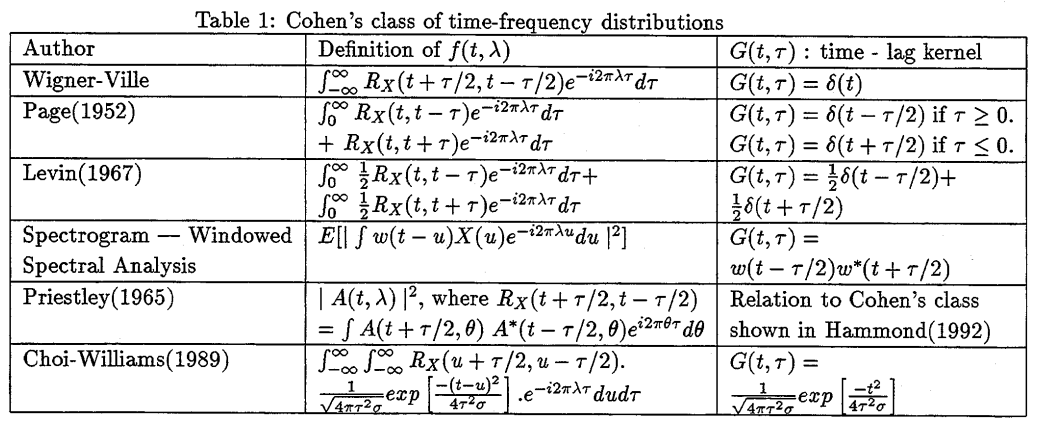
\includegraphics[width=0.9\textwidth]{tabla.png} 
\end{figure}

%Dos identidades muy importantes para estimar el espectro son la \textit{equivalencia} entre
%el espectro y la funci\'on de autocorrelaci\'on

%\begin{equation*}
%f(\omega ) = \int R_X(\tau ) e^{-i 2\pi \omega t} d\tau
%\end{equation*}
%
%Donde funci\'on de autocorrelaci\'on se ha definido como
%
%\begin{equation*}
%R_X(\tau) = E\left[ X(t) X(t+\tau) \right] = \int_0^{\infty} X(t)X(t+\tau) dt
%\end{equation*}
%
%[la demostracion es corta, batsa con reescribir una composicion de integrales como convolucion,
%la incluire mas tarde]
%
%Por otro lado, se tiene la Identidad de Parseval
%
%\begin{equation*}
%\int X^{2}(t) dt = \int f(\omega) d\omega
%\end{equation*}

%[esta demostracion se basa en la convergencia dominada del modulo de la integral de $X^{2}$ por
%la integral del modulo (...), la incluire mas tarde]

%%%%%%%%%%%%%%%%%%%%%%%%%%%%%%%%%%%%%%%%%%%%%%%%%%%%%%%%%%%%%%%%%%%%%%%%%%%%%%%%%%%%%%%%%%%%%%%%%%%

\subsection{Test Priestley-Subba Rao (PSR)}

%(seccion en proceso de re-redaccion)

A muy grosso modo, el test PSR estima localmente  el espectro evolutivo
 y revisa si estad\'isticamente
cambia en el tiempo.

Para ello, usa un estimador para la funci\'on de densidad espectral
que es aproximadamente (asint\'oticamente) insesgado y cuya varianza est\'a
determinada aproximadamente. La estimaci\'on se lleva a cabo en puntos en el tiempo y
la frecuencia tales que en conjunto son aproximadamente no-correlacionados.
Se aplica logaritmo para que la varianza de todos los estimadores sea aproximadamente
la misma (el logaritmo ayuda a), amen que los errores conjuntos tengan una
distribuci\'on cercana a una multinormal con correlaci\'on cero.
Finalmente se aplica una prueba ANOVA de varianza conocida.

%%%%%%%%%%%%%%%%%%%%%%%%%%%%%%%%%%%%%%%%%%%%%%%%%%%%%%%%%%%%%%%%%%%%%%%%%%%%%%%%%%%%%%%%%%%%%%%%%%%

\subsection{El espectro evolutivo}

Consid\'erese un proceso estoc\'astico a tiempo continuo $\{X(t)\}$, tal que
$E[X(t)]=0$ y $E\left[ X^{2}(t)\right] < \infty$ para todo $t$. Es decir que su media es constante
y sus segundos momentos est\'an bien definidos, aunque 
estos \'ultimos pueden cambiar con el tiempo.

Por el momento se supondr\'a que acepta una representaci\'on de la forma

\begin{equation*}
X(t) = \int_{-\pi}^{\pi} A(t ; \omega) e^{i\omega t} \, d Z(\omega)
\end{equation*}

Con $\{ Z(\omega) \}$ una familia de procesos ortogonales\footnote{De nuevo, esto implica que
$\Cov{dZ(\omega_1,dZ(\omega_2))} = \delta(\omega_1,\omega_1) d\omega$, una condici\'on m\'as
d\'ebil que la independencia} tales que

\begin{itemize}
\item $E \left[\abso{ dZ(\omega)}^{2} \right] = d\omega$
\item Para cada $t$ el m\'aximo de $A(t;\cdot)$ se encuentra en 0
\end{itemize}

Esta representaci\'on es an\'aloga a la representaci\'on de Cram\'er para un proceso
estacionario, salvo que se permite que la funci\'on $A$ cambie con el tiempo.
Siguiendo la analog\'ia, se define 
el \textbf{espectro evolutivo} de $\{X(t)\}$, con respecto a la la familia
$\mathcal{F} = \{ e^{i\omega t} A(t; \omega) \}$
 como
 
\begin{equation*}
d F(\omega;t) = \lvert A(t;\omega) \lvert^{2} d\omega
\end{equation*}

Ahora bien, si se supone que $\{X(t)\}$ es estoc\'asticametne diferenciable, entonces
se puede definir una \textbf{funci\'on de densidad espectral}

\begin{equation*}
f(t;\omega) = \lvert A(t;\omega) \lvert^{2}
\end{equation*}

Cabe destaca que si la funci\'on $A(t;\omega)$ fuera constante con respecto a $t$, se obtendr\'ia
un proceso estacionario de orden dos tal cual fue descrito en la secci\'on anterior.

%%%%%%%%%%%%%%%%%%%%%%%%%%%%%%%%%%%%%%%%%%%%%%%%%%%%%%%%%%%%%%%%%%%%%%%%%%%%%%%%%%%%%%%%%%%%%%%%%%%

\subsection{El estimador de doble ventana}

Esta t\'ecnica fue presentada por Priestley en 1965. Muy a grosso modo, es un estimador de la
funci\'on de densidad espectral con ciertas propiedades y que parte de la idea que un proceso
no-estacionario puede verse localmente como un proceso lineal generalizado.

Como meta-nota, yo empec\'e a estudiar este tipo de estimadores porque es \textit{el qeu ven\'ia
con el m\'etodo} ya que el test esta implementado en R; desde un punto de vista de difusi\'on,
es una ventaja usar un m\'etodo implementado en un software gratuito y de c\'odigo abierto --y
no una mera excusa para no explorar otros m\'etodos. En todo caso, he revisado varios otros test,
pero de momento solo este ha arrojado suficientes resultados para llenar un informe.

%{Estimador de doble ventana (Priestley, 1965 \& 1966)}
Para construir el estimador se reuieren dos funciones, $g$ y $w_T$, que servir\'an como ventanas
para extraer informaci\'on local de los datos. Debido a que sus propiedades tienen una interpretaci\'on
f\'isica desde la teor\'ia de circuitos, absorben su terminolog\'ia

\textit{
nota al pie: deberia incluir una motivacion de estos nombres,
que en parte tiene relevancia en la interpretacion. Los 
Linear Invariant Systems (LIS) suponen dependencia lineal
--constante-- respecto a todos los tiempos anteriores; 
a tiempo continuo son equivalentes a una ecuacion diferencial ordinaria lineal,
y a su vez a modelos AR. Un modelo fisico para ello son los circuitos RC, que
fueron usables en radios, y para los cuales las palabras 'filtro' y 'frecuencia'
tienen una interpretacion clara. Esta terminologia de circuitos electricos tiene sentido
para mi ya que todos los modelos de neuronas y poblaciones de neuronas que he visto hasta ahora,
por ejemplo de Ermentrout (falta citar), {Clark98,Priestley81}, PARTEN de considerar
circuitos equivalentes a los componentes neuronales, lo cual me hace pensar que es buena idea
mantener esta vision conjunta.
}

Primeramente se toma una funci\'on $g(u)$ normalizada, que en conjunto a su
transformada inversa de Fourier\footnote{Esta funci\'on 
$\Gamma(u) = \int_{-\infty}^{\infty} g(u) e^{i u \omega} du$
es referida como
\textbf{frequency-response function}, nombre tiene un poco de encanto cuando
$g$ adopta ciertas formas particulares (senos y cosenos).} 
$\Gamma$ tiene las siguientes propiedades

\begin{equation*}
2\pi \int_{-\infty}^{\infty} \lvert g(u) \lvert^{2} du 
= 
\int_{-\infty}^{\infty} \lvert \Gamma(\omega) \lvert^{2} d\omega
= 1
\end{equation*}


A partir de $g$ y $\Gamma$ se define el filtro $U$ como una convoluci\'on
con las realizaciones del proceso

\begin{equation*}
U(t,\omega) = \int_{t-T}^{t} g(u) X({t-u}) e^{i \omega (t-u)} du
\end{equation*}

Un ejemplo que est\'a en el libro de Priestley es tomar funciones del tipo

\begin{equation*}
g_h(u) = 
\begin{cases}
{1 \big{/} 2\sqrt{\pi h}} & \text{ , } \abso{u} \leq h
\\
0 & \text{ , } \abso{u} > 0
\end{cases}
\end{equation*}

Su correspondiente funci\'on de respuesta de frecuencia es complicada [me falta 
escribirla]. Es referida como la \textbf{ventana de Bartlett} y
est\'a totalmente caracterizada la siguiente propiedad

\begin{equation*}
\abso{\Gamma_h(\omega)}^{2} = \frac{1}{\pi h} \left( \frac{\text{sen} (h \omega)}{\omega} \right)^{2}
\end{equation*}

Cabe mencionar que puede entenderse al par $g$ y $\Gamma$ como ventanas en el tiempo
y las frecuencias para la serie.

---

Ahora bien, se toma una segunda ventana $W_\tau$ con las siguientes
restricciones para
su funci\'on de respuesta ante frecuencia $w_\tau$

\begin{itemize}
\item $w_{\tau}(t) \geq 0$ para cualesquiera $t$, $\tau$
\item $w_{\tau}(t) \rightarrow 0$ cuando $\lvert t \lvert \rightarrow \infty$, para todo $\tau$
\item $\displaystyle \int_{-\infty}^{\infty} w_{\tau}(t) dt = 1$ para todo $\tau$
\item $\displaystyle \int_{-\infty}^{\infty} \left( w_{\tau}(t) \right)^{2} dt < \infty$ para todo $\tau$
\item Existe una constante $C$ tal que  [T est\'a relacionado con el 'tiempo 0', pero para
tiempos de muestreo grandes se puede reemplazar por $-\infty$ EXCEPTO cerca del inicio y el final dle muestreo]
$$\lim_{\tau\rightarrow\infty} \left[ \tau \int_{t-T}^{t} \lvert W_{\tau}(\lambda) \lvert^{2} d\lambda \right] = C$$
\end{itemize}

%Ahora, si se define 
%$\displaystyle W_{T'}(\lambda) = \int_{-\infty}^{\infty} e^{-i\lambda t}w_{T'}(t) dt $

[posteriormente annadire mas detalles sobre el papel que juega el par $w_\tau$, $W_\tau$]

Como ejemplo, se puede tomar la siguiente funci\'on llamada \textbf{ventana de Daniell}

\begin{equation*}
W_\tau (t) = 
\begin{cases}
{1 \big{/} \tau} & \text{ , } -\nicefrac{1}{2} \tau \leq t \leq \nicefrac{1}{2} \tau
\\
0 & \text{ , otro caso}
\end{cases}
\end{equation*}

La cual se puede demostrar [tengo en algun lado esa demostracion]

$$\lim_{\tau\rightarrow\infty} \left[ \tau \int_{t-T}^{t} \lvert W_{\tau}(\lambda) \lvert^{2} d\lambda \right] = 2\pi$$

-----

Se define el estimador para $f_t$, con $0 \leq t \leq T$
\begin{equation*}
\widehat{f_t}(\omega) = \int_{t-T}^{t} w_{T'}(u) \lvert U(t-u,\omega) \lvert^{2} du
\end{equation*}

Fue demostrado por Priestley (1965, falta citar) que 

[aqui van las expresiones para el valor esperado y la varianza de $\widehat{f_t}$, me falta
escribirlas]

Pero, bajo varios supuesto adicionales [que me falta trascribir] se puede aproximar

\begin{equation*}
E\left[ \widehat{f_t}(\omega) \right] \sim f_t(\omega)
\end{equation*}

\begin{equation*}
\Var{\widehat{f_t}(\omega)} 
\sim 
\frac{C}{\tau} \left(f_t(\omega)\right)^{2} \int_{-\infty}^{\infty} \abso{\Gamma(\theta)}^{4} d\theta
\end{equation*}

Se advierte claramente que $\widehat{f_t}$ es unnestimados aproximadamente insesgado.
Para las ventanas de Bartlett y Daniell usadas como ejemplo, se tiene

\begin{equation*}
\Var{\widehat{f_t}} 
\sim 
\frac{4h}{3\tau} \left(f_t(\omega)\right)^{2}
\end{equation*}

Cabe mencionar que hay una expresi\'on expl\'icita para la covarianza de $\widehat{f_t}$
en para diferentes puntos en el tiempo y las frecuencias. Lamentablemente,
aun me falta escribirlas, son complicadas, y se describen situaciones bajo las
cuales estas covarianzas son negligibles; cabe destacar que TODAS las condiciones 
que se usan para aproximar son b\'asicamente las mismas, y dependen de que la distancia
entre los tiempos y las frecuencias sean tan grandes como sea posible.

------------

El \'ultimo ingrediente del test PSR es una transformaci\'on logar\'itmica
para regular la varianza, y quiza para cortar los bordes de las aproxiamciones.
Se define $Y_{i,j} = \log \left( \widehat{f_{t_i}}(\omega_j) \right)$, con las siguientes propiedades

\begin{equation*}
E\left[ Y_{i,j} \right] \thicksim \log \left( f_{t_i}(\omega_j) \right)
\hspace{4em}
\text{Var}\left( {Y\left(t,\omega\right)}\right) \thicksim \sigma^{2}
\end{equation*}

Luego as\'i, puede escribirse aproximadamente que

$$Y_{i,j} = \log \left( f_{t_i}(\omega_j) \right) + \varepsilon_{i,j}$$

donde $\varepsilon_{i,j}$ va iid tales que

$
E\left[ \varepsilon_{i,j} \right] = 0
\hspace{4em}
\text{Var}\left( \varepsilon_{i,j} \right) \sigma^{2}
$

Priestley cita que con esta informaci\'on incluso se puede considerar que los $\varepsilon_{i,j}$
siguen una distribuci\'on normal cada uno; Nason (2015, falta citar) comenta que
este supuesto no tiene por que cumplirse, y que es una popsible fuente de falsos positivos
para el test. Yo he hecho pruebas de normalidad a los datos, que incluire como anexos
mas tarde.

El test PSR \textit{per se} son tres test ANOVA --en su versi\'on en la que la varianza es conocida--
sobre si los $\varepsilon_{i,j}$ son estad\'isticamente negligibles en total, sobre el tiempo y sobre
las frecuencias. Para el fin de estudiar la estacionariedad, basta con que sean estad\'iticamente
no-negligibles sobre el tiempo.

[Por supuesto que los otros dos test tienen interpretacion: la negigibilidad total da informacion
sobre las marginales, y si estas pueden ser estimadas adecuadamente usando el estimador, si se
combina con negativo para no-estacionariedad es \textbf{efectivamente positivo} para estacionariedad
y toma una forma muy particular (proceso uniformemente modulado). Si sobre las frecuencias resulta
significativo (no-negligible) da informacion sobre la 'aeatoridad total' del proceso.
De tener tiempo, lo incluire como anexo, ya que ninguna de estas caracteristicas es estudiada :( ]

Lo detalles de la implementaci\'on en R estar\'an en la secci\'on de resultados.

%%%%%%%%%%%%%%%%%%%%%%%%%%%%%%%%%%%%%%%%%%%%%%%%%%%%%%%%%%%%%%%%%%%%%%%%%%%%%%%%%%%%%%%%%%%%%%%%%%%
%%%%%%%%%%%%%%%%%%%%%%%%%%%%%%%%%%%%%%%%%%%%%%%%%%%%%%%%%%%%%%%%%%%%%%%%%%%%%%%%%%%%%%%%%%%%%%%%%%%

\section{Conceptos, matem\'aticas}

En esta secci\'on se describen los conceptos b\'asicos de la teor\'ia espectral 'cl\'asica' para 
procesos estacionarios, y la generalizaci\'on hecha por Priestley para procesos no-estacionarios. 
De forma m\'as bien pragm\'atica, la descripci\'on est\'a
 fuertemente inspirada por el libro 'Spectral Analysis and Time Series' 
de M. B. Priestley \cite{Priestley81}, ya que este est\'a expl\'icitamente dirigido a un p\'ublico 
sin un trasfondo matem\'atico.

Se suponen conocidos varios temas b\'asicos de probabilidad y estad\'istica:
variables aleatorias, valores esperados y momentos, estimadores y sus propiedades.
Sin embargo, con el fin de presentar la notaci\'on usada, se incluyen algunos 
%conceptos previos a la 
%definici\'on per se de estacionariedad y estimadores en el dominio de frecuencias.
de estos conceptos.
%Chatfield (The Analysis of Time Series: An Introduction, 2003)

%%%%%%%%%%%%%%%%%%%%%%%%%%%%%%%%%%%%%%%%%%%%%%%%%%%%%%%%%%%%%%%%%%%%%%%%%%%%%%%%%%%%%%%%%%%%%%%%%%%

\subsection{Estacionariedad d\'ebil}

Para hablar formalmente de procesos estoc\'asticos como modelos, antes 
conviene escribir su definici\'on desde el punto de vista matem\'atico. Las siguientes definiciones
son aplicables tanto para procesos en tiempo continuo
como para procesos a tiempo discreto; aunque el objeto de estudio, el EEG, se considera 
un fen\'omeno continuo, s\'olo es posible registrarlo durante un conjunto finito de puntos 
en el tiempo.

\begin{defn}[Proceso estoc\'astico]
Un proceso estoc\'astico $\{ X(t) \}$ es una familia de variables aleatorias 
en los reales,
indexadas por
$t \in T \subseteq \R$.
%, mientras que una observaci\'on
%de $\{X(t)\}$ ser\'a denotada por $(x_1,x_2,\dots)$
\end{defn}

Como notaci\'on, una realizaci\'on de $X(t)$ ser\'a denota por $x_t$. 
Las funciones de densidad de probabilidad y de probabilidad acumulada para $X(t)$ ser\'an
referidas, respectivamente, como $f_{X(t)}$ y $F_{X(t)}$
%Cabe destacar que en esta definici\'on se omiti\'o intencionalmente pedir que las variables
%aleatorias sea reales, ya que eventualmente se considerar\'an procesos en los complejos.
Cabe enfatizar que para cada valor de $t$,
%tiempo $t$, 
$X(t)$ es una variable aleatoria; no se presupone ninguna conexi\'on entre ellas.
%con su funci\'on de densidad de probabilidad,
%sus momentos [s\'olo se consideran va's con al menos segundos momentos finitos], etc.


La caracter\'istica principal 
investigada en este trabajo hace referencia a la ''estacionariedad''. De manera 
informal, esta propiedad se refiere a que las variables aleatorias que conforman un proceso
estoc\'astico sean b\'asicamente iguales --dicho con otras palabras, que las propiedades
del proceso sean invariantes en el tiempo. 
Una definici\'on que satisface fielmente est\'a descripci\'on es la de estacionariedad 
en el sentido fuerte o estricto.
El t\'ermino ''tiempos admisibles'' simplemente indica que la definici\'on es la misma para
procesos a tiempo discreto o continuo, bajo restricciones obvias.

\begin{defn}[Estacionariedad fuerte]
Un proceso estoc\'astico $\{ X(t) \}$ es fuertemente estacionario si, para cualquier 
conjunto de tiempos admisibles $t_1,t_2,\dots,t_n$ y cualquier $\tau$ tal que 
 $t_i+\tau$ son tiempos admisibles para $i = 1, 2, \dots n$;
se cumple que
\begin{equation*}
F_{\left(X(t_1),X(t_2),\dots,X(t_n)\right) }
\equiv
F_{\left(X(t_1+\tau),X(t_2+\tau),\dots,X(t_n+\tau)\right)}
\end{equation*}

Donde $F_{\left(X(t_1),X(t_2),\dots,X(t_n)\right) }$ es la funci\'on de distribuci\'on de
probabilidad conjunta del vector $\left(X(t_1),X(t_2),\dots,X(t_n)\right)$
\end{defn}

Esta definici\'on, sin embargo, no resulta muy \'util en el contexto de la estad\'istica:
si se supone que el registro de un fen\'omeno puede interpretarse como \textbf{una} 
realizaci\'on de
un proceso estoc\'astico, entonces para cada tiempo se tiene una \'unica observaci\'on
de cada variable aleatoria. A esto hay que a\~nadir que, para un fen\'omeno continuo,
no todas los tiempos son registrables.
Luego, si no existe la garant\'ia de que las propiedades de estas variables aletorias sean
''similares'', entonces es virtualmente imposible obtener mayor informaci\'on de ellas.

Es bajo estas limitaciones que se motiva un concepto de estacionariedad m\'as d\'ebil, pero que
satisfaga ''suficientes teoremas importantes'' y que sea relevante bajo las restricciones
propias de diferentes campos. En este trabajo se ha optado por la llamada 
''estacionariedad d\'ebil'' o estacionariedad de orden 2, que recibe su nombre como caso
particular de la ''estacionariedad de orden $m$''.

\begin{defn}[Estacionariedad de orden $m$]
Un proceso estoc\'astico $\{ X(t) \}$
se dice estacionario de orden $m$ si, para cualquier 
conjunto de tiempos admisibles $t_1,t_2,\dots,t_n$ y cualquier $\tau \in \R$
se cumple que
\begin{equation*}
\E{ X^{m_1}(t_1)X^{m_2}(t_2)\cdots X^{m_n}(t_n) }
=
\E{ X^{m_1}(t_1+\tau)X^{m_2}(t_2+\tau)\cdots X^{m_n}(t_n+\tau) }
\end{equation*}
Para cualesquiera enteros $m_1,m_2,\dots,m_n$ tales que $m_1+m_2+\dots+m_n \leq m$
\label{est_orden_m}
\end{defn}

La estacionariedad d\'ebil no pide que la funci\'on
de distribuci\'on conjunta tenga determinada forma, sino que los momentos conjuntos sean 
invariantes ante traslaciones en el tiempo. Para entender mejor esta diferencia, consid\'erense
tres procesos $\{X(t)\}$, $\{Y_1(t)\}$ y $\{Y_2(t)\}$, de modo que el primero es
estacionario en el sentido fuerte, el segundo es estacionario de orden 1 y el tercero es
estacionario de orden 2.
\begin{itemize}
\item Por definici\'on $F_{X(t) } \equiv F_{X(t+\tau)}$ para cualesquieras $t$, $t+\tau$
admisibles; entonces $\E{X(t)} = \mu_X$ es constante
\item Por definici\'on
para cualesquieras $t$, $t+\tau$ admisibles se tiene que $\E{Y_1(t)}=\E{Y_1(t+\tau)}$ y
$\E{Y_2(t)}=\E{Y_2(t+\tau)}$. Se deduce que $\E{Y_1(t)} = \mu_{Y_1}$, 
$\E{Y_2(t)} = \mu_{Y_2}$ son constantes
\item Usando nuevamente que $F_{X(t) } \equiv F_{X(t+\tau)}$ para cualesquieras $t$, $t+\tau$
admisibles, se deduce que $\Var{X(t)} = \sigma_X$ es constante
\item Por definici\'on de $\mathrm{Var}$ y de $Y_i$ ($i=2,1$)
$$\Var{Y_i(t)} = \E{Y_i^{2}(t)} - \left( \E{Y_i(t)} \right)^{2} = \E{Y_i^{2}(t)} - \mu_{Y_i}$$
Luego se puede deducir que 
$\Var{Y_2(t)}$ es
% $\E{Y_2^{2}(t)}$ es
constante, mientras que no se puede garantizar lo mismo para $\Var{Y_1(t)}$
% Se concluye que la varianza
%de $Y_2$ es constante en el tiempo mientras que la de $Y_1$ no necesariamente lo es
\item El \textit{coeficiente de asimetr\'ia de Fisher} 
de una variable aleatoria $V$ se define como
$$
\gamma_1(V) = \frac{\E{\left(V-\E{V}\right)^{3}}}{\Var{V}^{\nicefrac{3}{2}}}
$$
%= \frac{\E{X^{3}}-3\mu_V \E{V^{2}}+2\mu_V^{3}}{\Var{V}^{\nicefrac{3}{2}}}
%$$
Sin entrar en detalles, se puede deducir que $\gamma_1(X(t))$ es constante mientras que no se
puede garantizar lo mismo para $\gamma_1(Y_1(t))$, $\gamma_1(Y_2(t))$
\end{itemize}

Naturalmente hay una relaci\'on de contenci\'on clara en
la familia de los conjuntos de procesos estacionarios de orden finito:
si un proceso es estacionario de orden $m$, entonces es estacionario de orden $n$ para todo
$n \leq m$. Es posible incluso describir procesos que sean estacionarios de orden ''infinito''
y preguntarse bajo qu\'e condiciones son fuertemente estacionarios.
Tal discusi\'on no se incluye en el presente trabajo.
%,
%% con el fin de ser concreto.
%ya que 
%%el enfoque es de modelaci\'on y 
%se ha intentado hacer la menor cantidad posible de supuestos y de proporcionara a cada uno una
%''interpretaci\'on fisiol\'ogica''.


%As\'i pues, y dadas 
Una vez hechas
las consideraciones anteriores, conviente
introducir una segunda caracter\'izaci\'on de los procesos estacionarios de orden 2 --d\'ebilmente 
estacionarios--
% enlistar las siguientes propiedades para un proceso
%estacionario de orden 2 --o d\'ebilmente estacionario-- 
que es equivalente
%\footnote{Este hecho se vuelve claro si se analizan cuidadosamente las propiedades
%enlistadas y se comparan con las deficiniones de las ''cantidades'' involucradas}
a la definici\'on \ref{est_orden_m} pero cuya interpretaci\'on suele considerarse como m\'as clara
%Hay una especie de consenso seg\'un el cual la estacionariedad de orden 2, tambi\'en
%llamada \textbf{estacionariedad d\'ebil} es suficiente para
%que se cumplan los teoremas m\'as comunes sobre medias y varianzas.
%Algunas consecuencias que un
%proceso sea estacionario debilmente son las siguientes:
\begin{thrm}
Un proceso es d\'ebilmente estacionario si y s\'olo si para cualesquiera tiempos admisibles
$t$, $s$ se tiene que
\begin{itemize}
\item $\E{X(t)} = \mu_X$
\item $\Var{X(t)} = \sigma^{2}_X$
\item $\Cov{X(t),X(s)} = \rho (s-t)$
\end{itemize}
Donde $\mu_X$, $\sigma^{2}_X$ son constantes, $\rho(\tau)$
es una funci\'on que \'unicamente depende de $\tau$
\label{est_usual}
\end{thrm}

%A grosso modo, cuando uno se refiere a un proceso d\'ebilmente estacionario seg\'un
%\ref{est_orden_m} se le pide que su primer y segundo momentos sean constantes, as\'i como
%el primer momento conjunto s\'olo dependa del lag en el tiempo. A su vez, seg\'un 
%\ref{est_usual} un proceso es d\'ebilmente estacionario si su media y varianza son constantes en
%el tiempo, y su funci\'on de autocovarianza s\'olo depende del lag en el tiempo.

Cabe mencionar, como comentario, que es posible contruir procesos que sean fuertemente
estacionarios pero que no sean estacionarios de ning\'un orden finito; dado que
la primera definici\'on se basa en funciones de densidad de probabilidad mientras que la segunda
se basa en momentos, es suficiente con usar variables aleatorias que no tengan todos
sus momentos bien definidos. Por ejemplo, consid\'erese un proceso conformado por variables
aleatorias independientes id\'enticamente distribuidas con distribuci\'on de Cauchy.

Dado que en el EEG se miden fluctuaciones en potenciales de campos el\'ectricos
%(medida en mV),
y que en este trabajo son modelados como variables aleatorias, 
la intepretaci\'on usual para los momentos de estas variables est\'a ligado a la distribuci\'on de
energ\'ia asociada al sistema. Luego, es plausible considerar que el EEG es un fen\'omeno
''suficientemente regular'' como para que las variables aleatorias del modelo tengan cuando
menos segundos momentos bien definidos; m\'as adelante discutir\'a un poco m\'as sobre por
qu\'e es importante este suspuesto.

%%%%%%%%%%%%%%%%%%%%%%%%%%%%%%%%%%%%%%%%%%%%%%%%%%%%%%%%%%%%%%%%%%%%%%%%%%%%%%%%%%%%%%%%%%%%%%%%%%%

\subsection{Espectro de un proceso estacionario}

Existe una larga tradici\'on en las ciencias biom\'edicas para interpretar a los registros
electrofisiol\'ogicos en t\'erminos de ondas y frecuencias, ya que fundamentalmente se
trata de fen\'omenos el\'ectricos \cite{Kaiser00}. 
As\'imismo existe una teor\'ia matem\'atica bien desarrollada sobre estad\'istica en el 
llamado ''dominio de las frecuencias''. 
En este trabajo se aborda la segunda como forma de tener coherencia con la primera; a continuaci\'on
se describen los conceptos m\'as importantes en el modelo usado.

Un objeto fundamental para el estudio del dominio de las frecuencias\footnote{Este concepto 
no se
%discutir\'a en el presente trabajo, sino que 
ser\'a manejado pragm\'aticamente para referirse
al cambio de coordenadas inducido por la transformada de Fourier o alguna generalizaci\'on de la 
misma} son las series de Fourier y sus generalizaciones. 

\begin{defn}[Serie de Fourier]
Sea $f$ una funci\'on peri\'odica con periodo $2\pi$ tal que $\intR \abso{f(t)} dt < \infty$. 
Si se calculan los coeficientes
\begin{equation*}
A_n = \frac{1}{2\pi} \intPI f(t) e^{- i n t} dt
\end{equation*}
entonces la siguiente igualdad se cumple casi en todas partes
\begin{equation*}
f(x) = \sum_{n=-\infty}^{\infty} A_n e^{i n t}
\end{equation*}
La sucesi\'on $\left( A_n \right)$ ser\'a referida como \textbf{serie de Fourier} de la funci\'on
$f$.
\label{FourierClasico}
\end{defn}

%\begin{defn}[Transformada de Fourier (funciones peri\'odicas)]
%Sea $f$ una funci\'on peri\'odica con periodo $2\pi$ tal que $\intR \abso{f(t)} dt < \infty$.
%hjkjkjkj
%\end{defn}

Por el momento no se discutir\'an los detalles sobre la convergencia de las sucesiones de 
\ref{FourierClasico}, siempre que se limite a funciones 
peri\'odicas,
continuas y absolutamente sumables,
%$L^{1}\left([-\pi,\pi])\right)$
o se permita que sean acotadas y con
una cantidad finita de discontinuidades --y se ponga ninguna atenci\'on sobre ellas.
Parece claro que se puede definir una funci\'on --quiz\'a invertible-- que mapee funciones 
a sus respectivas series de Fourier;
%que
%poseen serie de Fourier a ''alg\'un'' conjunto de series absolutamente sumables $\ell$; 
esta
funci\'on es referida como \textbf{transformada de Fourier}. Por lo pronto se considerar\'a
que las propiedades y limitaciones de la transformada de Fourier son conocidas
al menos a grosso modo, m\'as que nada por brevedad; se pretende exhibir
el espectro de potencias para una serie de tiempo como una extensi\'on de la
transformada de Fourier de modo que se espera
poder enfatizar sobre algunas
interpretaciones dentro de la modelaci\'on.
%conocidas y demostradas todas sus propiedades.

%%%%%%%%%%%%%%%%%%%%%%%%%%%%%%%%%%%%%

\subsubsection{Notas sobre interpretaci\'on f\'isica}

Las series de Fourier gozan de una interpretación física muy extendida como que una 
se\~nal\footnote{Esta palabra se usar\'a para referirse a un fen\'omeno f\'isisco 
que est\'a siendo 
registrado, bajo el entendido que es casi lo mismo referirse al registro o al proceso
que lo genera si \'este es determinista}
peri\'odica
puede verse como la superposici\'on de se\~nales peri\'odicas m\'as simples. 
De igual forma es destacable su interpretaci\'on como ''coordenadas'' en un espacio de funciones
dada una base ortonormal del mismo. 
El estudio de estos espacios dentro del an\'alisis trae a la mente
la cuesti\'on de convergencia,
el problema del subespacio de
funciones medibles de medida cero, y la posibilidad de otras bases; estos fen\'omenos tienen a su 
vez una interpretaci\'on f\'isica como cambios s\'ubitos en la energ\'ia, el ruido y la 
tipificaci\'on de ondas ''simples'' --por ejemplo, las ondas cuadradas y triangulares son 
m\'as comunes en teor\'ia de circuitos.

Para limar estas ambig\"uedades, en este trabajo se considerar\'a la base de Fourier como la
''m\'as natural'' por su conexi\'on simple con las exponenciales complejas. El t\'ermino
''ruido'' ser\'a evitado en la medida de lo posible ya que, en la terminolog\'ia de se\~nales,
suele referirse a registros con un comportamiento err\'atico y poco
predecible; dentro del contexto de electrofisiolog\'ia, tal descricpi\'on bien
puede englobar tanto
se\~nales que
se desea estudiar, como interferencias y errores.
%Para los procesos estoc\'asticos que son considerados en este trabajo, 
Conviene definir
un tipo de ''regularidad estoc\'astica'' que sirva para distinguir los patrones buscados
de errores de medici\'on e interferencias.

\begin{defn}[Continuidad estoc\'astica (media cuadr\'atica)]
Un proceso estoc\'astico a tiempo continuo $\{ X(t) \}$ es estoc\'asticamente continuo
(en el sentido de media cuadr\'atica)
en un tiempo admisible $t_0$ si y s\'olo si
\begin{equation*}
\lim_{t \rightarrow t_0} \E{\left( X(t) - X(t_0) \right)^{2}} = 0
\end{equation*}
\label{cont_est}
\end{defn}

Una forma natural de pensar en la definici\'on \ref{cont_est} es esperar que en promedio
$\lim_{t \rightarrow t_0} \left( X(t) - X(t_0) \right)^{2} = 0$. 
No es la \'unica forma de presentar un l\'imite de variables aletorias, sino que se ha elegido
esta forma por algunas propiedades que ser\'an explotadas m\'as adelante. 
As\'imismo cabe destacar que un proceso estoc\'asticamente continuo no necesariamente produce 
realizaciones que son funciones continuas, sino que sus realizaciones deben ser continuas 
casi en todas partes\footnote{Una funci\'on es \textit{continua casi en todas partes} si
es continua en todo su dominio excepto por un conjunto de medida cero}.

%%El arquetipo de esta clase de procesos es el proceso de Wiener.
%%%
%%%Por ejemplo, un proceso de Poisson es estoc\'asticamente continuo aunque sus realizaciones
%%%nunca son continuas; un proceso ruido blanco (variables aleatorias indepentiendes
%%%e id\'enticamente distribuidas)
%%%no es estoc\'asticamente continuo ya que puede 
%%%
%%%Para explorar este concepto de manera concreta, consid\'erese un proceso de Wiener; como es 
%%%un ejemplo ''r\'apido'', se definir\'a a apartir de sus propiedades:
%%%
%%%\begin{defn}[Proceso de Wiener]
%%%Un proceso estoc\'astico a tiempo continuo $\{ W(t) \}$ recibe el nombre de proceso
%%%de Wiener si satisface que
%%%\begin{itemize}
%%%\item $W(0) = 0$
%%%\item La variable aleatoria $W(t) - W(s)$ tiene una distribuci\'on normal con media 0 y 
%%%varianza $\abso{t-s}$
%%%\item Las variables aleatorias ${W(t)}$ y ${W(t) - W(s)}$ son independientes para
%%%todos los tiempo permitidos $t$, $s$
%%%\end{itemize} 
%%%\end{defn}
%%%
%%%Ahora bien, se considera un proceso de Wiener $\{W(t)\}$ con $t\geq 0$, y se verificar\'a su 
%%%continuidad estoc\'astica para un punto arbitrario $t_0 > 0$. 
%%%Por definici\'on, se tiene
%%Para mostrarlo, consid\'erese un proceso de Wiener $\{W_t\}$; 
%%por su definici\'on se tiene que
%%$$W(t) - W(t_0) \sim N(0,\abso{t-t_0}) \sim \sqrt{\abso{t-t_0}} N(0,1)$$
%%donde el s\'imbolo $\sim$ indica que dos variables tienen la misma funci\'on de densidad de 
%%probabilidad. Luego, como $ \left( W(t) - W(t_0) \right)^{2} \sim \chi^{2}(1) $, se cumple que
%%$$
%%\E{\left( W(t) - W(t_0) \right)^{2}}
%%$$
%%y luego entonces es claro que $\lim_{t \rightarrow t_0} \E{\left( X(t) - X(t_0) \right)^{2}} = 0$.
%%Esta aritm\'etica de variables aleatorias puede formalizarse, pero a lo largo de
%%este trabajo se supondr\'an conocidos los detalles respectivos.

De manera m\'as general, cabe mencionar un teorema que permite tipificar de manera m\'as
adecuada esta clase de procesos.

\begin{thrm}
Un proceso d\'ebilmente estacionario a tiempo continuo es estoc\'asticamente continuo si y s\'olo si
su funci\'on de autocorrelaci\'on es continua en 0
\end{thrm}
%\begin{demostracion}
%Sea $\{ X(t) \}$ un proceso d\'ebilmente estacionario, y sea $t_0$ un tiempo admisible arbitrario. 
%Luego, para todo $t$ admisible se cumple que
%\begin{align*}
%\E{\left( X(t) - X(t_0) \right)^{2}}
%&= \Var{X(t)} + \Var{X(t_0)} - 2 \Cov{X(t)}{X(t_0)}
%\\
%&= 2 \sigma_X^{2} \left( 1 - \rho(t-t_0) \right)
%\end{align*}
%donde $\rho$ es la funci\'on de autocorrelaci\'on y $\sigma_X^{2}$ la varianza del proceso. 
%Luego es claro que
%\begin{align*}
%\lim_{t\rightarrow t_0} \E{\left( X(t) - X(t_0) \right)^{2}} = 0  
%&{\Leftrightarrow}
%\lim_{t\rightarrow t_0} 2 \sigma_X^{2} \left( 1 - \rho(t-t_0) \right) = 0
%\\
%&{\Leftrightarrow}
%\lim_{\tau \rightarrow 0} \rho(\tau) = 1
%\end{align*}
%Como siempre se cumple que $\rho(0)=1$, la condici\'on final se traduce en que $\rho$ sea continua 
%en 0
%\end{demostracion}

Con esta segunda caracterizaci\'on a la mano, es f\'acil afirmar que un proceso %donde todas
%conformado por variables aleatorias independientes 
ruido blanco
no es estoc\'asticamente continuo,
ya que su funci\'on de autocorrelaci\'on vale 0 en todos los puntos
excepto en 0, donde vale 1. 
El proceso de Wiener, en cambio, es el arquetipo de un proceso estoc\'asticamente continuo.

En este trabajo se supondr\'a que los registros de PSG corresponden a realizaciones
de procesos estoc\'asticamente continuos; se considera la posiblidad de que est\'en
''contaminados'' por ''ruidos'', entendidos como procesos independientes de los potenciales de 
campo 
en el cerebro, de amplitud negligible y que ''muy posiblmente'' son estoc\'asticamente discontinuos 
casi en todas partes.

%---------------------------------------------------------------------------------------------------

Con respecto al concepto de energ\'ia, en este trabajo se usar\'a 
%formalmente desde un resultado
%usual, que se tomar\'a como definici\'on: 
desde la interpretaci\'on usual de teor\'ia de circuitos, pero que formalmente fungir\'a 
como definici\'on:
la energ\'ia disipada por la se\~nal $f$ 
%en el intervalo
%de tiempo $(t_1,t_2)$
est\'a dada por la expresi\'on \ref{energia}; si se divide tal expresi\'on
por $T$ se obtiene la \textit{potencia} (energ\'ia por unidad de tiempo)

%\begin{definition}[Energ\'ia y potencia de una se\~nal]
%
%\end{definition}

\begin{equation}
\int_{-T}^{T} \abso{f\left(t\right)}^{2} dt
\label{energia}
\end{equation}

%En este contexto
Vale la pena mencionar que este concepto de energ\'ia, como 
integral
%aporte conjunto
de una forma cuadr\'atica, es com\'un a varias ramas de la f\'isica y se encuentra ampliamente
extendido en las ingenier\'ias; en la econom\'ia, en cambio, no hay una motivaci\'on clara para
hacer uso de este concepto. 
Las t\'ecnicas electrofisi\'ologicas, concebidas dentro de la teor\'ia de circuitos, hereda la
terminolog\'ia e interpretaci\'on de energ\'ia.
%de modo que en 
En
este trabajo no s\'olo se contempla
como ''muy natural'' la idea de energ\'ia en los campos el\'ectricos del cerebro, sino que se
supondr\'a que esta es acotada para cualquier intervalo finito.
%Despu\'es de todo, el an\'alisis espectral tiene sus orignes en la f\'sicia, 

Contemplando este panorama, conviene se\~nalar
una relaci\'on cl\'asica entre la energ\'ia de una se\~nal
peri\'odica y su serie de Fourier (teorema \ref{parseval_serie});
tal idea ser\'a de gran importancia posteriormente en este trabajo.  

\begin{defn}[Relaci\'on de Parseval (funciones peri\'odicas)]
Sea $f$ una funci\'on peri\'odica de periodo $2T$ tal que acepta una representaci\'on como serie
de Fourier
\begin{equation*}
f(x) = \sum_{n=-\infty}^{\infty} A_n e^{i n t}
\end{equation*}
con $A_n = \frac{1}{2\pi} \intPI f(t) e^{- i n t} dt$. Entonces se cumple que
\begin{equation*}
\int_T^{T} X^{2}(t) dt = \sum_{n=-\infty}^{\infty} \abso{A_n}
\end{equation*}
\label{parseval_serie}
\end{defn}

Aunque esta afirmaci\'on
es relativamente simple desde la \'optica del An\'alisis funcional, tiene una interpretaci\'on
f\'isica importante: si una se\~nal puede descomponerse como una transposici\'on (suma) de 
se\~nales ortogonales simples, entonces su energ\'ia debe ser la suma de las energ\'ias 
asociadas a cada una de estas se\~nales. M\'as a\'un, un cambio en alguna de las se\~nales
ortogonales (base) afecta a la cantidad total de energ\'ia --pero no a las otras se\~nales base.
Incluso,
la independencia de las se\~nales base sugiere que la energ\'ia puede ser tratada separadamente
para cada se\~nal base. Luego, el m\'odulo de la serie de Fourier indica de cierto modo
c\'omo se distribuye la energ\'ia (o potencia) sobre las se\~nales base; por esta raz\'on se le
suele referir como \textbf{espectro de potencia}\footnote{Dada esta discusi\'on, conviene 
distinguir el \textit{espectro de potencia no-normalizado} como la energ\'ia definida como
en \ref{energia} usando \ref{parseval_serie}, mientras que un \textit{espectro de potencia 
normalizado} se puede definir de la misma forma pero diviendo la expresi\'on en 
\ref{energia} por $2T$}.

%---------------------------------------------------------------------------------------------------

%En el contexto de series electrofisiol\'ogicas, se mencion\'o que en el EEG se han descrito y
%patrones llamados ''ondas de sue\~no'' \footnote{Para m\'as informaci\'on ver
%las secciones anteriores}. Hist\'oricamente estas ondas fueron tipificados mediante el 
%uso de registros electroencefalogr\'aficos en papel, de modo que se define emp\'iricamente
%la ''frecuencia'' de una onda se sue\~no al contar el n\'umero de altibajos en una unidad
%de tiempo \cite{Klonowski09}. En un plano muy formal, no se espera que una onda  de sue\~no
%tenga una transformada de Fourier, al menos en el sentido cl\'asico; por otro lado, se espera que
%pueda formalizarse el concepto de una onda ''parecida'' a unacua frecuencia es tal.

En este caso, se presentar\'a la transformada de Fourier-Stieltjes. En primera instancia
%permite frecuencias puntuales que son inconmensurables con respecto al intervalo $[-\pi,'pi]$,
%de modo que 
acepta funciones no-peri\'odicas pero que pueden ser representadas como suma de funciones
peri\'odicas, la diferencia m\'as notable es que permite involucar funciones cuya frecuencia
es inconmensurable con respecto al intervalo $[-\pi,\pi]$ como por ejemplo la funci\'on
$$
f(x) = \COS{x} + \COS{x\sqrt{2}}
$$
no tiene una serie de Fourier, pero puede ser representada como una integral de Fourier-Stieltjes.

%---------------------------------------------------------------------------------------------------

Dicho esto, conviene indagar sobre las propiedades de las
funciones involucradas en una
transformada de Fourier-Stieltjes: no-negativas, monotonamente crecientes; si se habla de funciones
con energ\'ia finita se puede tambi\'en asegurar que son acotadas.
%son similares a una 
La transformada de Fourier-Stieltjes es una medida en alg\'un espacio --el nombre daba
algunas pistas al respecto. 
%--el nombre da pistas al respecto.

Si bien, dentro de la interpretaci\'on f\'isica, parece muy
la caracterizaci\'on de la transformada de Fourier-Stieltjes como una medida en alg\'un espacio 
--que posiblemente est\'e asociado a la distribuci\'on de energ\'ia--, desde el punto de vista
formal tiene consecuencias bastante interesantes.
Por ejemplo, basta citar un corolario del teorema de separaci\'on de Lebesgue (escrito
como \ref{Lebesgue_decomp}) seg\'un el cual una funci\'on con ciertas caracter\'isticas se puede 
separar como suma de tres funciones: una ''muy regular'', una ''compuesta \'unicamente por 
saltos'' y un residuo con ''propiedades extravagantes''.

\begin{thrm}[Descomposici\'on de Lebesgue]%, fun. de variaci\'on acotada]
Sea $f:I\rightarrow \R$ una funci\'on de variaci\'on acotada, con $I$ un intervalo. Entonces
pueden hallarse funciones $f_j, f_c, f_a :I\rightarrow \R$ tales que
\begin{itemize}
\item $f = f_j+ f_c+ f_a$
\item $f_j = \sum_{y \leq x} f(x-0) + f(x+0)$
\item $f_a$ es absolutamente continua\footnote{Para que una funci\'on sea absolutamente continua,
basta que sea de variaci\'on acotada y que mapee conjuntos de medida cero en conjuntos de medida
cero} en $I$
\item $f_c$ es una funci\'on singular\footnote{Una funci\'on es singular si es continua, 
de variaci\'on acotada y no-constante, y se cumple que tiene derivada cero casi en todas partes} 
en $I$
\end{itemize}
Estas funciones son \'unicas excepto por constantes, y en conjunto son llamados la 
\textit{descomposici\'on de Lebesgue} de $f$
\label{Lebesgue_decomp}
\end{thrm}

Una vez mencionado el teorema \ref{Lebesgue_decomp}, combinado con el hecho de que las funciones de 
distribuci\'on de probabilidad
son de variaci\'on acotada, implica que --en cierto sentido-- una variable aleatoria se puede
''descomponer'' como una variable aletoria discreta, una variable aleatoria continua y una
variable aleatoria patol\'ogica; por brevedad no se profundizar\'a m\'as sobre ello.
Dado que la transformada de Fourier tiene propiedades similares a una funci\'on de distribuci\'on,
el aplicar el teorema \ref{Lebesgue_decomp} sobre ella da pie a descomponer una funci\'on
que admite una transformada de Fourier-Stieltjes como suma de tres funciones: una
con espectro discreto, una con espectro continuo, y una funci\'on patol\'ogica.

Dentro del contexto de electrofisiolog\'ia, en este trabajo se supone
que una se\~nal puede descomponerse
como suma de dos funciones, una con espectro discreto --que tiene una serie de Fourier cl\'asica--
y otra con espectro continuo --que se estimar\'a como derivada de ''algo''.
Este supuesto equivale a que la ''componente'' patol\'ogica del espectro es negligible.

%---------------------------------------------------------------------------------------------------

%%%%%%%%%%%%%%%%%%%%%%%%%%%%%%%%%%%%%

\subsubsection{Espectros estoc\'asticos}

Una pregunta natural cuando se toma la terminolog\'ia de ondas y frecuencias dentro
del estudio de series de tiempo, es sobre el significado de aplicar la transformada de Fourier a
un proceso estoc\'atico --o cuando menos a alguna sus realizaciones.
¿Bajo qu\'e condiciones las realizaciones de un proceso estoc\'astico admiten una representaci\'on
como series/integrales de Fourier/Fourier-Stieltjes?

%(Por simplicidad se abordar\'a primero esta pregunta para procesos a tiempo continuo, y 
%posteriormente se tratar\'a el caso a tiempo disreto.)

Se sabe que una condici\'on suficiente para que exista la transformada de Fourier de una funci\'on
dada, es que pertenezca al espacio de las funciones cuadrado-integrables, $L^2$.
%, definido como
%$
%L^2(\R) = \left\{ f: \R \rightarrow \R {\biggr\rvert} \int_{-\infty}^{\infty} f(x) dx < \infty \right\}
%$

Sin embargo, considerando un proceso estacionario $\{ X(t) \}$, y dado que tiene varianza constante 
en el tiempo, se 
espera que sus realizaciones $x(t)$ no decaigan en infinito. Tampoco hay garant\'ia
que admitan una representaci\'on de Fourier-Stieltjes. M\'as a\'un, no hay garant\'ia alguna que
una realizaci\'on arbitraria pueda expresarse como la suma de una funci\'on en $L^2$ y una
funci\'on que admita representaci\'on de Fourier-Stieltjes.

El enfoque que se aborda es construir una sucesi\'on de funciones 
%peri\'odicas 
en $L^{2}$
que convergen a ''cada'' realizaci\'on
$x(t)$, y luego revisar la convergencia de sus respectivas integrales de Fourier.
As\'i entonces, para cada $T>0$ se define
\begin{equation}
x_T(t) = 
\begin{cases}
x(t) & \text{ , } -T\leq t \leq T
\\
0 & \text{ , otro caso}
\end{cases}
\end{equation}

Claramente, para todo $T$ se tiene que $x_T \in L^2$, y entonces la siguiente 
representaci\'on est\'a bien definida
\begin{equation}
x_T (t) = \frac{1}{\sqrt{2 \pi}} \intR G_T(\omega) e^{i \omega t} d\omega
\end{equation}

Donde se define la funci\'on $G_T$ como

\begin{equation}
G_T (\omega) = \frac{1}{\sqrt{2 \pi}} \intR x_T(t) e^{-i \omega t} dt
= \frac{1}{\sqrt{2 \pi}} \int_{-T}^{T} x(t) e^{-i \omega t} dt
\end{equation}

Como se mencion\'o anteriormente, no hay garant\'ia de que $x(t)$, una realizaci\'on arbitraria de
$\{X(t)\}$, tenga una integral de Fourier bien definida. Luego entonces no hay garant\'ia que 
$G_T$ converja cuando $T\rightarrow \infty$. Recuperando la interpretaci\'on de 
$\left| G_T(\omega) \right|^{2}$ como una funci\'on de distribuci\'on para la energ\'ia total del sistema 
%asociada a la frecuencia
sobre las frecuencias
puntualse $\omega$, destaca un argumento f\'isico seg\'un el cual $G_T$ {deber\'ia} diverger:
durante un tiempo infinito, un sistema que maneja ''niveles constantes'' de 
energ\'ia puede registrar una cantidad infinita de energ\'ia en su historial. 
%Curiosamente,
%esta segunda interpretaci\'on del
%problema motiva una soluci\'on para el mismo: usando un tipo de promedio para la
%distribuci\'on de energ\'ia involucrando a $T$

Este problema puede remediarse 
%resolviendo el enredo de palabras y t\'erminos, 
siguiendo la interpretaci\'on f\'isica del objeto que se intenta investigar:
%ya que 
no es tan importante la
cantidad total de energ\'ia 
sobre todos los tiempos posibles, ya que s\'olo es importante lo que ocurra en intervalos finitos
de tiempo.
%concentrada en cada frecuencia, 
%sino qu\'e frecuencias concentran m\'as
%energ\'ia. 
Luego entonces conviene usar un promedio que 
%''tome en cuenta'' el tama\~no
%del intervalo
involucre el tama\~no de los intervalos ''recortados'' y que pueda converger a una suerte de 
densidad de energ\''ia en el tiempo.

\begin{equation}
\lim_{T\rightarrow{\infty}} = \frac{ \left| G_T(\omega) \right|^{2}}{2 T}
\label{yacasi}
\end{equation}

La expresi\'on en \ref{yacasi} es una adaptaci\'on de la integral de Fourier para una realizaci\'on
de un proceso estoc\'astico a tiempo continuo; los detalles sobre la convergencia de esta 
cantidad se discutir\'an m\'as adelante;
cabe destacar que la forma en que se promedia s\'olo resulta significativa para procesos estacionarios.
%conserva una parte clave de la interpretaci\'on.
Por mientras, y en cierta medida, se ha contestado una de las interrogantes 
%al inicio de esta 
previas
%secci\'on 
sobre la posibilidad y
el significado de una transformada de Fourier para las realizaciones de un proceso 
estoc\'astico; con respecto a la posibilidad de una transformada para el proceso per se, vale la 
pena
ajustar la definici\'on en \ref{yacasi} para que sea ''representativa'' del proceso --y no s\'olo
de una realizaci\'on particular. Priestley introduce la siguiente funci\'on

\begin{equation}
h(\omega) = \lim_{T\rightarrow \infty} \E{ \frac{ \left| G_T(\omega) \right|^{2}}{2 T} }
\end{equation}

La funci\'on $h$ es referida como la \textit{funci\'on de densidad espectral no-normalizada} para
$\{X(t)\}$. Posteriormente se definir\'a una versi\'on ''normalizada'' de la SDF.
%, pero antes debe
%definirse la ''potencia total'' del proceso; por simplicidad, antes de ello se exhibir\'an
%algunas propiedades de la SDF, adem\'as algunos teoremas importantes.

La discuci\'on sobre la convergencia de $h$ se omiti\'o por tiempo y simpleza de la explicaci\'on,
%aunque basta con intentar aplicar la definici\'on \ref{SDF} a una funci\'on determinista
%continua y peri\'odica --puede interpretarse como un proceso estoc\'astico degenerado, 
%con varianza 0
%para cualquier tiempo permitido. 
%Como toda funci\'on peri\'odica continua posee una serie de Fourier bien definida, la SDF del
%proceso debe ''coincidir'' en cierto sentido. 
%Desde la interpretaci\'on f\'isica, tiene sentido que la energ\'ia de una se\~nal peri\'odica
%debe estar distribuida entre se\~nales peri\'odicas --caso contrario, sus ''modos'' ser\'ian
%imcompatibles y perder\'ian energ\'ia al interactuar--; luego la distribuci\'on de energ\'ia
%debe tener picos tipo ''delta de Dirac'' en las frecuencias compatibles.
ya que es posible un proceso con espectro discreto o mixto (una idea similar a una funci\'on 
con espectro discreto, pero con sus diferencias obvias):
un proceso cuya SDF no est\'a bien definida en 
todos sus puntos, pero tal que estos puntos no pueden ser ignorados.
En parte, el objetivo de la discusi\'on sobre la integral de Fourier-Stieltjes es que parezca
natural definir un la integral de la SDF, el \textbf{espectro integrado} $H$
\begin{equation*}
H(\omega) = \lim_{T\rightarrow \infty} 
\E{ \frac{1}{2 T} \left| \intR G_T(\omega\prima) d\omega\prima \right|^{2} }
\end{equation*}

De manera completamente an\'aloga al caso en que la transformada de Fourier-Stieltjes puede
interpretarse como una medida, $H$ tambi\'en puede ser vista como una medida; m\'as a\'un,
siempre que $h(\omega)$ est\'e bien definida puede decirse que 
$\frac{dH(\omega)}{d\omega}= h(\omega)$ --una analog\'ia interesante con que la funci\'on
de densidad de probabilidad es la derivada de la funci\'on de probabilidad acumulada siempre
que la segunda sea derivable.
No se discutir\'a con detalle am\'en de no repetir, pero $H$ es positiva, no-decreciente y
acotada para condiciones que se discutir\'an m\'as adelante.

%%%%%%%%%%%%%%%%%%%%%%%%%%%%%%%%%%%%%%%%%%%%%%%%%%%%%%%%%%%%%%%%%%%%%%%%%%%%%%%%%%%%%%%%%%%%%%%%%%%

\subsection{Estimaci\'on de la funci\'on de densidad espectral}

En la subsecci\'on anterior se exhibi\'o una forma de definir un espectro de potencias para 
procesos estoc\'asticos estacionarios --hasta ahora se ha supuesto que tienen cuando menos
segundos momentos finitos. Esta definici\'on es resumida en \ref{SDF} para el caso no-normalizado;
como el operador $\mathrm{E}$ indica el valor esperado sobre todas las realizaciones del proceso,
la definici\'on se hescribi\'o en t\'erminos del proceso y no de sus realizaciones.

\begin{defn}[Funci\'on de densidad espectral (SDF) no-normalizada]
Sea $\{X(t)\}$ un proceso estoc\'astico at iempo continuo, d\'ebilmente estacionario. Se define
la funci\'on de densidad espectral (SDF) de $\{X(t)\}$ como
%a tiempo continuo 
%tal que para todo tiempo admisible $t$ se cumple que $\E{X(t)}$
\begin{equation*}
h(\omega) = \lim_{T\rightarrow \infty} \E{ \frac{ \left| G_T(\omega) \right|^{2}}{2 T} }
\end{equation*}
Donde $G_T (\omega) = \frac{1}{\sqrt{2 \pi}} \int_{-T}^{T} X(t) e^{-i \omega t} dt$
\label{SDF}
\end{defn}

%Como se mencion\'o anteriormente, se omiti\'o intencionalmente una discusi\'on sobre el proceso hasta
%ahora. Y e

%Consid\'erese un ejemplo hip\'otetico de ondas cerebrales alfa de 10 Hz, donde el ruido externo 
%ha sido eliminado completamente; este registro te\'orico se 

%Desde el punto de vista matem\'atico, m\'as interesante,
%el conjunto de las funciones que tienen transformada de 
%Fourier bien definida es un subconjunto de las funciones que tienen transformada de
%Fourier-Stieltjes bien definida; si bien esto ya se hab\'ia mencionado anteriormente, conviene
%extender tal discusi\'on reflexionando sobre la estructura de este segundo espacio.
%
%Dada una serie de Fourier, se puede construir una funci\'on que posee una transformada de
%Fourier,
%%y dada una funci\'on acotada
%%mon\'otonamente creciente, se puede hacer lo equivalente; lo inte
%y, como buena generalizaci\'on, esta funci\'on tambi\'en posee una transformada de 
%Fourier-Stieltjes bien definida; basta tomar [continuar despues]

%Algo que salta a la vista de estas funciones con espectro discontinuo es que su SDF no est\'a
%bien definida en todos los puntos, al menos no como la derivada de la SDF integrada.
%Este fen\''omeno es b\'asicametn id\'entico al de las variables aleatorias discretas:
%su funci\'on
%de distribuci\'on de probabilidad acumulada es discontinua, luego no es cierto que su
%funci\'on de densidad de probabilidad sea la derivada ''de algo''.

%Se espera poder definir $h$ para funciones deterministas --no sólo para proceso estoc\'asticos--
%en el caso que exista una ''componente determinista'' que resulte ser importante; por ejemplo, los
%una presencia marcada de ondas cerebrales.

Es importante un comentario que imita a aqu\'el sobre la definici\'on de estacionariedad:
la definici\'on \ref{SDF} es sumamente ineficiente en t\'erminos de estimaci\'on, ya que implica
tomar un valor esperado sobre todas las posibles realizaciones del proceso.
En este caso se exhiben varios teoremas respecto a la SDF, y que permiten estimarla aprovechando
las regularidades de un proceso d\'ebilmente estacionario. 
En este sentido, son fundamentales los teoremas de Wiener-Khintchine y de Wold.

\begin{thrm}[Wiener-Khintchine]
Una condici\'on suficiente y necesaria para que $\rho$ sea una funci\'on de autocorrelaci\'on de 
alg\'un proceso estoc\'astico a tiempo continuo $\{X(t)\}$ estacionario y estoc\'asticamente 
continuo, es que exista una funci\'on $F$ que tenga las 
%mismas propiedades que una funci\'on de 
%densidad de probabilidad
siguientes propiedades
\begin{itemize}
\item Monotonamente creciente
\item $F(-\infty) = 0$
\item $F(\infty) = 1$
\end{itemize}
y tal que para todo $\tau \in \R$ se cumple que
\begin{equation*}
\rho(\tau) = \intR e^{i \omega \tau} dF(\omega)
\end{equation*}
\end{thrm}

\begin{thrm}[Wold]
Una condici\'on suficiente y necesaria para que $\rho$ sea una funci\'on de autocorrelaci\'on de 
alg\'un proceso estoc\'astico a tiempo discreto $\{X(t)\}$ estacionario
% y estoc\'asticamente 
%continuo, 
es que exista una funci\'on $F$ con las 
%mismas propiedades que una funci\'on de 
%densidad de probabilidad
siguientes propiedades
\begin{itemize}
\item Monotonamente creciente
\item $F(-\pi) = 0$
\item $F(\pi) = 1$
\end{itemize}
y tal que para todo $\tau \in \R$ se cumple que
\begin{equation*}
\rho(\tau) = \intPI e^{i \omega \tau} dF(\omega)
\end{equation*}
\end{thrm}

Una diferencia fundamental entre estos dos teoremas es que el primero se refiere a procesos a
tiempo continuo, mientras que el segundo se refiere a procesos a tiempo discreto; un caso de
particularmente interesante es el de procesos a tiempo continuo que son observados en puntos

Si bien no es claro que el teorema de Wiener-Khintchine, o su extensi\'on por Wold, tengan una
interpretaci\'on f\'sica clara, tienen una interpretaci\'on clave para los estimadores en el
dominio de las frecuencias:
la SDF normalizada es la transformada de Fourier-Stieltjes de la 
funci\'on de autocorrelaci\'on.
Intuitivamente, esto significa que un estimador ''muy natural'' para la SDF normalizada
%se puede construir 
%a partir del estimador para la funci\'on de autocovarianza, aplic\'andole alg\'un tipo
%de transformada de Fourier. 
%M\'as adelante se mostrar\'a que ello no es la mejor opci\'on, p
es la transformada de Fourier de la funci\'on de autocorrelaci\'on (estimada);
esta funci\'on se conoce como \textit{periodograma}. Se usar\'an, sin embargo, la funci\'on
de autocovarianza ($R$) ya que en teor\'ia s\'olo difiere de la funci\'on de autocorrelaci\'on
al ser multiplicada por una constante, pero en la pr\'actica esta cantidad es un par\'ametro m\'as
para ser estimado.

Conviene introducir, antes, el estimador ''est\'andar''
para la funci\'on de autocovarianza de un proceso
d\'ebilmente estacionario a tiempo continuo de media cero $\{ X(t) \}$, 
a partir de un conjunto de $N$ 
observaciones distribuidas uniformemente en el tiempo con separaci\'on $\Delta t$.
Por simplicidad, se denotar\'a a estas observaciones como $x_1, x_2 , \dots, x_N$ .
Ahora bien, 
por definici\'on se cumple la siguiente propiedad para la funci\'on de autocovarianza, $R$,
del proceso
%\begin{align*}
%\rho(\tau) 
%&= \E{X(0)X(\tau)} \\
%&= \E{X(\Delta t)X(\Delta t + \tau)} \\
%&= \E{X(2\Delta t)X(2\Delta t + \tau)} \\
%&= \cdots
%\end{align*}
\begin{equation*}
R(\tau)
= \E{X(n\Delta t)X(n\Delta t + \tau)} \text{  ,  } n = 0,\pm 1,\pm 2, \pm 3,\dots
\end{equation*}
para $n = 0, 1, 2, \dots, N$ y siempre que $\tau$ sea m\'ultiplo de
$\Delta t$. Luego, un estimador muy natural para $\rho$ est\'a dado por
\begin{equation}
\widehat{R}(\tau) = \frac{1}{N-\abso{\tau}} 
\sum_{t = 1}^{N-\abso{\tau}} x_t x_{t+\abso{\tau}}
\label{estimador_R}
\end{equation}

Resulta que $\widehat{R}$ es un estimador insesgado y consistente de $R$;
sin embargo y por simplicidad en un tratamiento futuro, 
conviene introducir un estimador sesgado para $R$ con algunas propiedades convenientes
\begin{equation}
\aste{R}(\tau) = \frac{1}{N} 
\sum_{t = 1}^{N-\abso{\tau}} x_t x_{t+\abso{\tau}}
\label{estimador_R_ast}
\end{equation}

Por tiempo s\'olo se citar\'a que --para un proceso d\'ebilmente estacionario-- el
estimador \ref{estimador_R_ast} tiene las siguientes propiedades
\begin{itemize}
\item $\E{\aste{R}(\tau)} = \left(1 - \frac{\abso{\tau}}{N} \right) R(\omega)$
\item $\Var{\aste{R}(\tau)} \approx \frac{1}{N} 
\sum_{r=-\infty}^{\infty} \left( R^{2}(r) + R(r-\tau)R(r+\tau) \right)$
%\item $\Cov{\aste{\rho}(\tau),\aste{\rho}(\tau+\nu)} \approx \frac{1}{N} 
%\sum_{r=-\infty}^{\infty} \left( \rho(r)\rho(r+\nu) + \rho(r-\tau)\rho(r+\tau+\nu) \right)$
\end{itemize}
La aproximaci\'on 
para la varianza se vuelve
exacta si el proceso es normal, aunque es asint\'otica en general.
%con el n\'umero de puntos.

As\'i entonces se puede definir, como se mencion\'o, 
el periodograma $I_N(\omega)$ de la siguiente manera

\begin{equation}
I_N(\omega) = 2 \sum_{r = -(N-1)}^{N-1} \aste{R}(r) \COS{r \omega}
\label{periodograma_rho}
\end{equation}

Ahora bien, la definici\'on cl\'asica del periodograma est\'a dada por la expresi\'on
en \ref{periodograma_rho}, 
aunque igualmente se puede definir por la expresi\'on equivalente
%y lo que pasa es que es equivalente a la definici\'on
en \ref{periodograma}; aunque la segunda es clara y efectiva computacionalmente, se usar\'a
la primera de manera recurrente.

\begin{equation}
I_N(\omega) = \frac{2}{N} \abso{ \sum_{t=0}^{N} e^{i \omega t} x_t }^{2}
\label{periodograma}
\end{equation}

%Para hablar de la media y varianza del periodograma, es fundamental distinguir el caso con
%espectro puramente discreto y el caso con espectro puramente continuo.
%En el primer caso, las siguientes formas fueron propuestas por Bartlet

Si bien se puede deostrar que en el caso continuo 
%se cumple que 
$\E{I_N(\omega)}=h(\omega)$, si el proceso tuviera un espectro puramente continuo,
ocurre que $\lim_{N\rightarrow 0} \Var{I_N(\omega)} = h^{2}(\omega)$. Luego el
periodograma ''cl\'asico'' --o cualquiera de sus formulaciones equivalentes-- es 
en general
un estimador
insesgado para la SDF, pero su varianza no decae a cero al incrementar el n\'umero de puntos;
intuitivamente esto sgnifica que en promedio se espera que funcione adecuadamente como
estimador, pero
%decir, 
aumentar la cantidad de datos no implica que la estimaci\'on mejore,%\footnote{La 
%demostraci\'on de esta propiedad es omitida por brevedad
%Este 
%comentario se puede hacer m\'as claro, pero no se ha hecho porque implica incluir m\'as material
%}.
y es muy posible que nunca sea realmente buena.

%Un problema indicao 
Priestley comenta que este efecto ocurre porque
%como comentario es que 
el periodograma --calculado seg\'un \ref{periodograma_rho}--
est\'a siendo depende de estimadores para la funci\'on de autocovarianza evaluada en todos los 
puntos accesibles; 
el problema con ello es que para evaluarla en retrasos m\'as grandes, 
%son calculados usando
se requieren puntos m\'as alejados, y como hay muy pocos disponibles
%generan una mayor varianza.
generan un estimador con varianza muy alta.

Puesto que el periodograma aumenta su varianza porque incluye las ''colas'' de la 
funci\'on de
autocovarianza, una respuesta cl\'asica 
%a este problema 
es tratar de evitar en lo posible estas
colas 
%elimin\'andolas o 
multiplicando por una funci\'on de pesos.
% que disminuya r\'apidamente.
En este sentido, se considerar\'an los estimadores con la siguiente forma

%%%%%%%%%%%%%%%%%%%%%%%%%%%%%%%%%%%%%%%%%
%%%%%%%%%%%%%%%%%%%%%%%%%%%%%%%%%%%%%%%%%

%Se considerar\'an los estimadores de la forma
\begin{equation}
\est{h}(\omega) = \frac{1}{2\pi} \sum_{s = -(N-1)}^{N-1} 
\lambda(s) \aste{R}(s) e^{i \omega t}
\label{ventaneando}
\end{equation}

donde $\lambda$ es la funci\'on que ''decae muy r\'apidamente'', y ser\'a referida como
\textbf{ventana de retrasos}. Para estudiar las propiedades de los estimadores
dle tipo \ref{ventaneando}, conviene reescribirlos como funci\'on directa del periodograma

\begin{equation*}
\est{h}(\omega) = \intPI I_N(\theta) W(\omega-\theta) d\theta
\end{equation*}
donde $W$ es la transformada de Fourier finita de $\lambda$
\begin{equation*}
W(\theta) = \frac{1}{2\pi} \sum_{s = -(N-1)}^{N-1} \lambda(s) e^{-is\theta}
\end{equation*}

Cabe destacar la forma que adopta $\est{h}$ como convoluci\'on del periodograma con la funci\'on
$W$, que bien puede interpretarse como que esta \'ultima funciona como una funci\'on de pesos
--exactamente como $\lambda$, pero en el ''dominio de las frecuencias. Por ello, $W$ es
referida como \textbf{ventana de retrasos}.
En la tabla \ref{ventanas} hay una lista corta de algunas ventanas propuestas.
%; en la tabla 
%\ref{ventaneando}
%se tienen sus respectivos valres esperados y varianzas.
Esta familia de estimadores
%, si bien tienen una varianza que deace a cero conforme aumenta el
%n\'umero de puntos, en promedio no convergen al valor deseado; 
son consistentes pero
sesgados, aunque son asint\'oticamente insesgados, ya que el sesgo disminuye conforme aumenta el
n\'umero de puntos.


\begin{SidewaysFigure}
\centering
\begin{tabular}{c}
\textbf{Algunas funciones tipo ventana}
\vspace{1em}
\end{tabular}
\begin{tabular}{c||c|c}
 & Ventana de retrasos & Ventana en las frecuencias \\
 \hline
  \hline
P. truncado & 
$\displaystyle
\lambda(s) = \begin{cases}
1 &\text{, si } \abso{s} \leq M \\
0 &\text{, otro caso}
\end{cases}$ &
$\displaystyle
W(\theta) = \frac{1}{2\pi} \frac{\SEN{(M+\frac{1}{2})\theta}}{\SEN{\nicefrac{\theta}{2}}}
=: D_M(\theta)$
\\
 \hline
Bartlet &
$\displaystyle
\lambda(s) = \begin{cases}
1-\nicefrac{\abso{s}}{M} &\text{, si } \abso{s} \leq M \\
0 &\text{, otro caso}
\end{cases}$ &
$\displaystyle
W(\theta) = \frac{1}{2\pi M} 
\left( \frac{\SEN{ \nicefrac{M\theta}{2}}}{\SEN{\nicefrac{\theta}{2}}} \right)^{2}
=: F_M(\theta)$
\\
 \hline
Daniell &
$\displaystyle
\lambda(s) = \frac{\SEN{\nicefrac{\pi s}{M}}}{\nicefrac{\pi s}{M}}$ &
$\displaystyle
W(\theta) = \begin{cases}
\nicefrac{M}{2\pi} &\text{, si } \abso{\theta} \leq \nicefrac{\pi}{M} \\
0 &\text{, otro caso}
\end{cases}$
\\
 \hline
Tukey-Hanning &
$\displaystyle
\lambda(s) = \begin{cases}
\nicefrac{1}{2}\left( 1+ \COS{\nicefrac{\pi s}{M}} \right) &\text{, si } \abso{s} \leq M \\
0 &\text{, otro caso}
\end{cases}$ &
$\displaystyle
W(\theta) = \frac{1}{4} D_M\left(\theta - \frac{\pi}{M} \right) 
+\frac{1}{2} D_M\left(\theta \right)
\frac{1}{4} D_M\left(\theta + \frac{\pi}{M} \right)$
\\
 \hline
Parzen &
$\displaystyle
\lambda(s) = \begin{cases}
1-6\left( \nicefrac{s}{M} \right)^{2} + 6\left( \nicefrac{\abso{s}}{M} \right)^{3} 
&\text{, si } \abso{s} \leq \nicefrac{M}{2} \\
2\left( 1 - \nicefrac{\abso{s}}{M} \right)^{3}
 &\text{, si } \nicefrac{M}{2} \leq \abso{s} \leq M \\
0 &\text{, otro caso}
\end{cases}$ &
$\displaystyle
W(\theta) = \frac{3}{8 \pi M^{3}} \left( 
\frac{\SEN{\nicefrac{M\theta}{4}}}{\nicefrac{1}{2}\SEN{\nicefrac{\theta}{2}}} 
\right)^{4}
\left( 1- \nicefrac{2}{3} \SEN{\nicefrac{\theta}{2}}^{2} \right)$
\\
 \hline
Bartlet-Priestley &
$\displaystyle
\lambda(s) = \frac{3M^{2}}{\left(\pi s\right)^{2} }
\left( \frac{\SEN{\nicefrac{\pi s}{M}}}{\nicefrac{\pi s}{M}} - \COS{\nicefrac{\pi s}{M}}
\right)
$ 
%$\displaystyle
%\lambda(s) = \frac{3M^{2}}{\left(\pi s)^{2}}
%$ 
&
$\displaystyle
W(\theta) = \begin{cases}
\frac{3M}{4\pi} \left( 1- \left(\frac{M \theta}{\pi} \right)^{2} \right)
&\text{, si } \abso{\theta} \leq \nicefrac{\pi}{M} \\
0 &\text{, otro caso}
\end{cases}$
\end{tabular}
\caption{Ejemplos de algunas ventanas que suavizan el periodograma, formando
estimadores consistente de la SDF para el caso de espectro puramente continuo.
Las funciones $F_M$ y $D_M$ toman los nombres respectivos de \textit{n\'ucelo de Fejer} y
\textit{N\'ucleo de Dirichlet} de orden $M$}
\label{ventanas}
\end{SidewaysFigure}

%\begin{table}
%\centering
%\begin{tabular}{c||c|c}
%Ventana & Sesgo & Grados de libertad equivalentes
%
%\end{tabular}
%\end{table}

%%%%%%%%%%%%%%%%%%%%%%%%%%%%%%%%%%%%%%%%%
%%%%%%%%%%%%%%%%%%%%%%%%%%%%%%%%%%%%%%%%%

%%%%%%%%%%%%%%%%%%%%%%%%%%%%%%%%%%%%%%%%%%%%%%%%%%%%%%%%%%%%%%%%%%%%%%%%%%%%%%%%%%%%%%%%%%%%%%%%%%%

\subsection{Representaci\'on de Wold-Cram\'er}

Una consecuencia de los teoremas de Wiener-Khintchine y de Wold, de la que no se hab\'ia hablado
en este trabajo, es poder caracterizar a los procesos d\'ebilmente estacionarios
con una cierta forma; esta representaci\'on ser\'a auxiliar para estimar la SDF.
Esta represetnaci\'on existe en virtud del teorema \ref{rep_espectral}, cuya demostraci\'on
no ser\'a incluida en este trabajo;
el lector interesado en tan imponente teorema puede referirse a \cite{Priestley81}.

\begin{thrm}
Sea $\{X(t)\}$ un proceso estoc\'astico a tiempo continuo d\'ebilmente estacionario
de media 0
y estoc\'asticamente continuo --en el 
sentido de media cuadr\'atica. Entonces, existe un proceso ortogonal $\{Z(\omega)\}$ tal que, para 
todo tiempo $\omega$ admisible, se puede escribir\footnote{La integral se encuentra definida en el
sentido de media cuadr\'atica.}
\begin{equation*}
X(t) = \intR e^{i t \omega} dZ(\omega)
\end{equation*}
Donde el proceso $\{Z(t)\}$ tiene las siguientes propiedades para todo $\omega$
\begin{itemize}
\item $\E{dZ(\omega)} = 0$
\item $\E{\abso{dZ(\omega)}^{2}} = dH(\omega)$
\item $\Cov{dZ(\omega),dZ(\omega^{\prime})} = 0 \Leftrightarrow \omega \neq \omega^{\prime}$
\end{itemize}
Donde $dH(\omega)$ la SDF integrada no-normalizada de $\{X(t)\}$
\label{rep_espectral}
\end{thrm}

La forma en que se escribe un proceso seg\'un el teorema \ref{rep_espectral} es referida como
{representaci\'on de Cram\'er}; en virtud del teorema de Wold, se puede tener una variante
del mismo teorema para series de tiempo a tiempo discreto, raz\'on por la cual
en sentido amplio se le refiere como \textbf{representaci\'on de Wold-Cram\'er}.

\subsubsection{Filtros lineales independientes del tiempo}

Los filtros  
lineales independientes del tiempo se describen aqu\'i por su importancia hist\'orica en la 
estimaci\'on anal\'ogica de las SDF,
%LTS se introducen por su importancia 
%hist\'orica 
%para la estimaci\'on espectral
%anal\'ogica tradicional dentro de la teor\'ia de circuitos --
aunque en este trabajo se presenta
una abstracci\'on m\'as pragm\'atica en cuanto a la estimaci\'on de la SDF.
Este tipo de filtros ser\'an referidos como filtros LTI (Linear Time-Invariant)
ya que se les pedir\'a que dependan linealmente de toda la se\~nal\footnote{Se
entiende que es una mapeo lineal que toma toda la se\~nal --entendida como funci\'on del tiempo--
y ''produce'' otra funci\'on del tiempo --que a su vez puede interpretarse como una segunda 
se\~nal. Cabe
destacar que formalmente es necesario que el mapeo sea lineal sobre las se\~nales, pero no es 
obligatorio que ''utilice'' todos los valores: no se le pide ser invertible, ni continuidad}
y que no dependan del tiempo. Luego entonces, deben tener la forma \ref{LTI}.
\begin{equation*}
Y(t) = \intR g(s) X(t-s) ds
\label{LTI}
\end{equation*}
%El nombre proviene de \textit{Linear Time-invariant Systems}, y en sus or\'igenes consiste en
%un circuito conformado por componentes ''lineales'' (resistencias, capacitores, repetidores),
%el cual se alimenta con la se\~nal a estudiar con el objetivo de medir en otro punto del
%circuito la se\~nal resultante; este circuito es referido como \textbf{filtro}.

N\'otese que un filtro como \ref{LTI} est\'a completamente determinado por la funci\'on $g$. 
Sobre el contexto hist\'orico mencionado, conviene mencionar la existencia de ''circuitos 
lineales'' cuya composici\'on permite modelarlos como filtros LTI; un ejemplo cl\'asico
son los circuitos RC, como el mostrado en \ref{rrcc} y que est\'a determinado por
$g(u) = \frac{1}{R C} \text{exp}\left( -\nicefrac{u}{R C} \right)$ --donde $R$ y $C$ son la
resistencia y capactiancia, respectivamente.

\begin{figure}
\centering
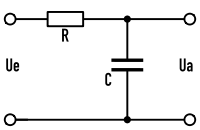
\includegraphics[width=0.4\linewidth]{rc.png} 
\caption{Circuito el\'ectrico con una resistencia (R) y un capacitor (C); es alimentado por
una corriente de entrada $V_e(t)$ y produce una corriente de salida $V_a(t)$. 
%Este circuito es un 
%ejemplo cl\'asico de circuito lineal, donde la corriente de salida est\'a dada por la expresi\'on
}
\label{rrcc}
\end{figure}

%Bajo las leyes de Kirchoff, el voltaje en todo punto de un ''circuito lineal'' viene dado
%por una ecuaci\'on diferencial lineal de orden finito, lo cual constituye una motivaci\'on
%m\'as clara para los elementos permitidos en ellos. De manera general, y omitiendo detalles,
%la se\~nal que ''sale'' de un filtro es una combinaci\'on lineal de todos los tiempos anteriores;
%%de manera general, 
%saltando algunos pasos m\'as,
%esta caracter\'istica puede expresarse como
%%puede expresarse como
%\begin{equation}
%Y(t) = \intR g(s) X(t-s) ds
%\label{LTS}
%\end{equation}

Se puede decir, por ejemplo, que para que un circuito sea ''f\'isicamente contruible'' es
necesario que $g$ sea cero en los negativos --que el valor actual no dependa de los valores
futuros. En este trabajo se pedir\'a que $g\in L^{2}$ y que posea una transformada de
Fourier bien definida.

%Donde $g$ es una funci\'on en $L^{2}$ tal que es cero para valores negativos\footnote{Esta
%propiedad se conoce como \textit{f\'isicamente realizable}, y destaca en el dise\~no de 
%filtros con propiedades especificadas}.

%De manera pragm\'atica, la introducci\'on sobre los circuitos LTS representa s\'olo un bosquejo,
%y se utilizar\'a la ecuaci\'on \ref{LTS} como definici\'on de los filtros LTS d\'andole
%el nombre de \textit{filtro} a la funci\'on $g$ siempre que est\'e en $L^{2}$.
%Una motivaci\'on para introducir este tipo de funciones es que los modelos est\'andar en 
%series de tiempo (AR, MA, ARMA, ARIMA) pueden ser entendidos en tiempo continuo como un filtro
%LTS aplicado a un proceso ruido blanco --por simplicidad, en este trabajo se entender\'a la integral
%en el sentido de media cuadr\'atica, y por el momento s\'olo ser\'a aplicada a procesos 
%d\'ebilmente estacionarios.

Una motivaci\'on muy fuerte para mencionar los filtros LTI es que permiten expresar de manera
''c\'omoda'' a los procesos est\'andares: un proceso MA 
%es el promedio de variables aleatorias
%independientes, aunque 
bien puede interpretarse como un filtro con forma de ventana rectangular
acotada, y esta caracterizaci\'on puede extenderse a tiempo continuo.
Un proceso AR en tiempo continuo se puede ver como una ecuaci\'on diferencial lineal y homog\'enea,
m\'as un proceso ruido blanco; este tipo de ecuaciones pueden interpretarse como circuitos lineales
--y por tanto, como filtros LTI-- antes de intetntar resolverse.
En esa direcci\'on, conviene considerar procesos de la forma
\begin{equation*}
Y(t) = \intR g(u) X(t) du
\end{equation*}
donde $g$ corresponde a un filtro LTI y $\{ X(t) \}$ es un proceso d\'ebilomente estacionario que
admite una representaci\'on de Wold-Cram\'er. Se puede mostrar que estas condiciones implican
que
\begin{equation*}
h_X(\omega) = h_Y(\omega) \abso{\Gamma(\omega)}^{2}
\end{equation*}
donde $h_X$ y $h_Y$ son las respectivas SDF de $\{X(t)\}$ y $\{Y(t)\}$, y 
$\Gamma(\omega) = \intR g(u) e^{i \omega u} du$.

La funci\'on $g$ es referida como \textbf{funci\'on de respuesta}; este nombre tiene sentido en la
interpretaci\'on de circuito si \'este es ''alimentado'' con un ''impulso unitario'' (una funci\'on
tipo \ddd de Dirac) en un tiempo dado, y posteriormente se mide la respuesta del sistema.
La funci\'on $\Gamma$ es referida como \textbf{funci\'on de transferencia}; su motivaci\'on
respectiva viene de realizar el mismo experimento te\'orico, pero ahora con una funci\'on
tipo $e^{i \omega t}$; el sistema producir\'a una funci\'on del tipo $e^{i\lambda t}$, que tiene
una forma similar pero con otra frecuencia. La conexi\'on de estas dos funciones se vuelve m\'as
clara a\'un si se interpretan las funciones del segundo experimento como funciones tipo
\ddd de Dirac en el especio de las frecuencias.

%%%%%%%%%%%%%%%%%%%%%%%%%%%%%%%%%%%%%%%%%%%%%%%%%%%%%%%%%%%%%%%%%%%%%%%%%%%%%%%%%%%%%%%%%%%
%%%%%%%%%%%%%%%%%%%%%%%%%%%%%%%%%%%%%%%%%%%%%%%%%%%%%%%%%%%%%%%%%%%%%%%%%%%%%%%%%%%%%%%%%%%

%Quiero y me siento obligado a citar la excelente discuci\'on
%filos\'ofica
%de Loynes \cite{Loynes68}, resaltando la frase ''Los espectros instant\'aneos no existen''.
%Tambi\'en quiero citar una discusi\'on m\'as moderna de M\'elard \cite{Melard89}, donde una
%frase a favor es ''El supuesto de estacionariedad ha sido v\'alido previamente debido a la corta
%duraci\'on de las series y la baja capacidad de c\'omputo''.

%\begin{equation*}
%X(t) = \int_{\Lambda} A(\omega) e^{i 2\pi \omega t} dZ(\omega)
%\end{equation*}
%
%Donde el proceso $\{ Z(\omega) \}$ tiene incrementos ortogonales, es decir 
%\begin{equation*}
%\Cov{dZ(\omega_1,dZ(\omega_2))} = \delta(\omega_1,\omega_1) d\omega
%\end{equation*}
%Con $\delta$ la funci\'on delta de Dirac. Cabe mencionar que es suficiente si los incrementos
%son independientes, pero se puede debilitar ese requerimiento; incluso es de notarse que no
%se exige que el proceso sea al menos continuo --en el sentido estoc\'astico.

%El espectro de potencia de $\{X(t)\}$ se define como
%
%\begin{equation*}
%f(\omega) = \abso{A(\omega)}^{2}
%\end{equation*}
%
%Citar\'e de Adak \cite{Adak98} una tabla donde compara varias definiciones de espectro, para
%procesos no-estacionarios.

%\begin{figure}
%\centering
%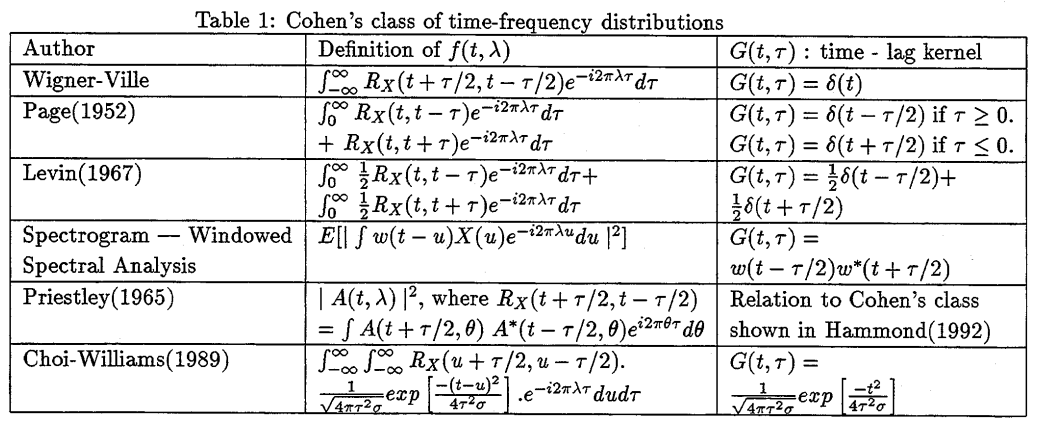
\includegraphics[width=0.9\textwidth]{tabla.png} 
%\end{figure}

%%%%%%%%%%%%%%%%%%%%%%%%%%%%%%%%%%%%%%%%%

%\subsection{Test Priestley-Subba Rao (PSR)}
%
%%(seccion en proceso de re-redaccion)
%
%A muy grosso modo, el test PSR estima localmente  el espectro evolutivo
% y revisa si estad\'isticamente
%cambia en el tiempo.
%
%Para ello, usa un estimador para la funci\'on de densidad espectral
%que es aproximadamente (asint\'oticamente) insesgado y cuya varianza est\'a
%determinada aproximadamente. La estimaci\'on se lleva a cabo en puntos en el tiempo y
%la frecuencia tales que en conjunto son aproximadamente no-correlacionados.
%Se aplica logaritmo para que la varianza de todos los estimadores sea aproximadamente
%la misma (el logaritmo ayuda a), amen que los errores conjuntos tengan una
%distribuci\'on cercana a una multinormal con correlaci\'on cero.
%Finalmente se aplica una prueba ANOVA de varianza conocida.

%%%%%%%%%%%%%%%%%%%%%%%%%%%%%%%%%%%%%%%%%%%%%%%%%%%%%%%%%%%%%%%%%%%%%%%%%%%%%%%%%%%%%%%%%%%%%%%%%%%

%\subsection{El espectro evolutivo}
%
%Consid\'erese un proceso estoc\'astico a tiempo continuo $\{X(t)\}$, tal que
%$E[X(t)]=0$ y $E\left[ X^{2}(t)\right] < \infty$ para todo $t$. Es decir que su media es constante
%y sus segundos momentos est\'an bien definidos, aunque 
%estos \'ultimos pueden cambiar con el tiempo.
%
%Por el momento se supondr\'a que acepta una representaci\'on de la forma
%
%\begin{equation*}
%X(t) = \int_{-\pi}^{\pi} A(t ; \omega) e^{i\omega t} \, d Z(\omega)
%\end{equation*}
%
%Con $\{ Z(\omega) \}$ una familia de procesos ortogonales\footnote{De nuevo, esto implica que
%$\Cov{dZ(\omega_1,dZ(\omega_2))} = \delta(\omega_1,\omega_1) d\omega$, una condici\'on m\'as
%d\'ebil que la independencia} tales que
%
%\begin{itemize}
%\item $E \left[\abso{ dZ(\omega)}^{2} \right] = d\omega$
%\item Para cada $t$ el m\'aximo de $A(t;\cdot)$ se encuentra en 0
%\end{itemize}
%
%Esta representaci\'on es an\'aloga a la representaci\'on de Cram\'er para un proceso
%estacionario, salvo que se permite que la funci\'on $A$ cambie con el tiempo.
%Siguiendo la analog\'ia, se define 
%el \textbf{espectro evolutivo} de $\{X(t)\}$, con respecto a la la familia
%$\mathcal{F} = \{ e^{i\omega t} A(t; \omega) \}$
% como
% 
%\begin{equation*}
%d F(\omega;t) = \lvert A(t;\omega) \lvert^{2} d\omega
%\end{equation*}
%
%Ahora bien, si se supone que $\{X(t)\}$ es estoc\'asticametne diferenciable, entonces
%se puede definir una \textbf{funci\'on de densidad espectral}
%
%\begin{equation*}
%f(t;\omega) = \lvert A(t;\omega) \lvert^{2}
%\end{equation*}
%
%Cabe destaca que si la funci\'on $A(t;\omega)$ fuera constante con respecto a $t$, se obtendr\'ia
%un proceso estacionario de orden dos tal cual fue descrito en la secci\'on anterior.

%%%%%%%%%%%%%%%%%%%%%%%%%%%%%%%%%%%%%%%%%%%%%%%%%%%%%%%%%%%%%%%%%%%%%%%%%%%%%%%%%%%%%%%%%%%%%%%%%%%

\subsection{El test de Priestley-Subba Rao}

Esta t\'ecnica fue presentada por Priestley y Subba Rao en 1965 \cite{Priestley69}; 
muy grosso modo, consiste en estimar el espectro
del proceso 
%en cuesti\'on 
''localmente en muchos lugares'',
y luego compararlos, revisando si se puede rechazar o no --como prueba de hip\'otesis-- 
%si se puede rechazar la hip\'otesis de que no
el que sean estad\'sticamente constantes en el tiempo.
%var\'ia en el tiempo.
%
%Para ello, usa un estimador para la funci\'on de densidad espectral
%que es aproximadamente (asint\'oticamente) insesgado y cuya varianza est\'a
%determinada aproximadamente. La estimaci\'on se lleva a cabo en puntos en el tiempo y
%la frecuencia tales que en conjunto son aproximadamente no-correlacionados.
%Se aplica logaritmo para que la varianza de todos los estimadores sea aproximadamente
%la misma (el logaritmo ayuda a), amen que los errores conjuntos tengan una
%distribuci\'on cercana a una multinormal con correlaci\'on cero.
%Finalmente se aplica una prueba ANOVA de varianza conocida.
%Muy a grosso modo, es un estimador de la
%funci\'on de densidad espectral con ciertas propiedades y que parte de la idea que un proceso
%no-estacionario puede verse localmente como un proceso lineal generalizado.
%Muy a grosso modo, 
Para ello 
supone que 
%localmente todo 
se est\'an lidiando con una cantidad finita de observaciones, provenientes de un
proceso estoc\'astico a tiempo continuo, \'este deber\'ia tener media cero y varianza 
finita en todo momento, adem\'as de ser estoc\'asticamente continuo y tener un espectro
puramente continuo.
% puede verse como un proceso lineal generalizado que es d\'ebilmente estacionario;
%luego se pueden usar las ventanas espectrales y los filtros LIS sobre una porci\'on 
%de tiempo ''peque\~na'' para estimar el espectro localmente.
Considerando estas hip\'otesis, describen los estimadores ''de doble ventana'', cuyas
propiedades permiten construir una prueba para detectar estacionariedad d\'ebil.

Cabe mencionar que anteriormente se presentaron
motivos por las cuales conviene considerar a las se\~nales del PSG como
estoc\'asticamente continuas y de varianza finita; la propiedad de tener media cero
y un espectro puramente continuo ser\'an ''forzadas'' llevando a cabo 
num\'ericamente
una descomposici\'on de
Lebesgue (definici\'on \ref{Lebesgue_decomp}) para las partes peri\'odicas y no-peri\'odicas
de cada registro, para lo cual se usar\'a el
algoritmo no-param\'etrico STL (ver m\'as adelante).



%Como meta-nota, yo empec\'e a estudiar este tipo de estimadores porque es \textit{el qeu ven\'ia
%con el m\'etodo} ya que el test esta implementado en R; desde un punto de vista de difusi\'on,
%es una ventaja usar un m\'etodo implementado en un software gratuito y de c\'odigo abierto --y
%no una mera excusa para no explorar otros m\'etodos. En todo caso, he revisado varios otros test,
%pero de momento solo este ha arrojado suficientes resultados para llenar un informe.

%{Estimador de doble ventana (Priestley, 1965 \& 1966)}
%El m\'etodo de estimaci\'on de doble ventana fue introducido por Priestley \cite{Priestley66} para
%procesos semi-estacionarios; 
%Para construir el estimador se requieren dos funciones, $g$ y $w_T$, que servir\'an como ventanas
%para extraer informaci\'on local de los datos. 
%Debido a que sus propiedades tienen una interpretaci\'on
%f\'isica desde la teor\'ia de circuitos, absorben su terminolog\'ia

%\textit{
%nota al pie: deberia incluir una motivacion de estos nombres,
%que en parte tiene relevancia en la interpretacion. Los 
%Linear Invariant Systems (LIS) suponen dependencia lineal
%--constante-- respecto a todos los tiempos anteriores; 
%a tiempo continuo son equivalentes a una ecuacion diferencial ordinaria lineal,
%y a su vez a modelos AR. Un modelo fisico para ello son los circuitos RC, que
%fueron usables en radios, y para los cuales las palabras 'filtro' y 'frecuencia'
%tienen una interpretacion clara. Esta terminologia de circuitos electricos tiene sentido
%para mi ya que todos los modelos de neuronas y poblaciones de neuronas que he visto hasta ahora,
%por ejemplo de Ermentrout (falta citar), {Clark98,Priestley81}, PARTEN de considerar
%circuitos equivalentes a los componentes neuronales, lo cual me hace pensar que es buena idea
%mantener esta vision conjunta.
%}

Con respecto a la estimaci\'on local del espectro, se usa el \textbf{estimador de doble ventana},
una t\'ecnica introducida por Priestley y Subba Rao \cite{Priestley69}.
Requiere que se proporcionen a priori dos funciones arbitrarias $w_\tau$ y $g$ que cumplan ciertas
propiedades; deber\'ian funcionar, respectivamente, como ventana de retrasos y como
filtro LTI.

%Primeramente se toma una funci\'on $g(u)$ normalizada, que en conjunto a su
%transformada inversa de Fourier
%%\footnote{Esta funci\'on 
%%$\Gamma(u) = \int_{-\infty}^{\infty} g(u) e^{i u \omega} du$
%%es referida como
%%\textbf{frequency-response function}, nombre tiene un poco de encanto cuando
%%$g$ adopta ciertas formas particulares (senos y cosenos).} 
%$\Gamma$ tiene las siguientes propiedades

En cuando a $g$ (as\'i como $\Gamma(u) = \intR g(u) e^{i u \omega} du$) se les pide que tengan 
integral normalizada, es decir
\begin{equation*}
2\pi \int_{-\infty}^{\infty} \lvert g(u) \lvert^{2} du 
= 
\int_{-\infty}^{\infty} \lvert \Gamma(\omega) \lvert^{2} d\omega
= 1
\end{equation*}

%Se puede entender a $g$ y $\Gamma$ como un filtro LTS que ''absorbe informaci\'on local''
%en el dominio de las frecuencias.
%A partir de $g$ y $\Gamma$ 
En base a ello se puede definir el siguiente estimador, que funciona no s\'olo como filtro del
proceso, sino como una aproximaci\'on un tanto burda de la representaci\'on de Wold-Cram\'er
para el 
proceso\footnote{Una segunda funci\'on de $U$, y que no se discutir\'a a fondo por brevedad, 
es ''aislar'' en los
valores de la SDF cercanos en el tiempo a aqu\'el unto donde se desea estimar.
Tambi\'en cabe mencionar que las ventanas espectrales mostradas en la tabla \ref{ventanas}
bien pueden cumplir las propiedades requeridas para ser filtros LTI.}
%Se define el filtro $U$ como una convoluci\'on
%con las realizaciones del proceso
\begin{equation*}
U(t,\omega) = \int_{t-T}^{t} g(u) X({t-u}) e^{i \omega (t-u)} du
\end{equation*}

%Un ejemplo que est\'a en el libro de Priestley es tomar funciones del tipo
%
%\begin{equation*}
%g_h(u) = 
%\begin{cases}
%{1 \big{/} 2\sqrt{\pi h}} & \text{ , } \abso{u} \leq h
%\\
%0 & \text{ , } \abso{u} > 0
%\end{cases}
%\end{equation*}
%
%Su correspondiente funci\'on de respuesta de frecuencia es complicada [me falta 
%escribirla]. Es referida como la \textbf{ventana de Bartlett} y
%est\'a totalmente caracterizada la siguiente propiedad
%
%\begin{equation*}
%\abso{\Gamma_h(\omega)}^{2} = \frac{1}{\pi h} \left( \frac{\text{sen} (h \omega)}{\omega} \right)^{2}
%\end{equation*}

%Cabe mencionar que puede entenderse al par $g$ y $\Gamma$ como ventanas en el tiempo
%y las frecuencias para la serie.

Bajo el entendido que la funci\'on $\Gamma$ converge a una funci\'on tipo $\delta$ de 
Dirac\footnote{La funci\'on $\delta_x:\R\rightarrow \R$ 
es una funci\'on $\delta$ de Dirac si puede verse como la funci\'on de distribuci\'on de masa
para una medida finita que es cero para todo conjunto que no contenga a $x$.
% si vale cero en
%todos los puntos excepto para $x$, y satisface que $\intR \delta_x(t) dt = k > 0$. 
Debido a estas propiedades, 
%conviene considerarlas como derivadas en el sentido de distribuci\'on
%dentro de integrales de Stieltjes. En 
en este trabajo no se les usar\'a directamente, sino que se les har\'a alusi\'on bien por su 
interpretaci\'on intuitiva (una masa concentrada en un s\'olo punto) o por que las funciones tipo
ventana suelen converger a funciones de este tipo}
puede considerarse que $\E{\abso{U(t,\omega)}^{2}} \approx f_t(\omega)$; sin embargo, se
demuestra en \cite{Priestley66} que $\Var{\abso{U(t,\omega)}^{2}} \nrightarrow 0$ como en el
caso del periodograma.

%---

Debido a ello es que se usa la segunda funci\'on, tipo ventana, para ''suavizar'' el estimador 
y hacerlo consistente
--de forma muy similar a como se usaron ventanas espectrales para suavizar el periodograma.
%que se usaron 
Se toma una funci\'on $W_\tau$ que tomar\'a el papel de ventana de retrasos,
con su respectiva ventana espectrasl $w_\tau$; se le piden las siguientes propiedades

\begin{itemize}
\item $w_{\tau}(t) \geq 0$ para cualesquiera $t$, $\tau$
\item $w_{\tau}(t) \rightarrow 0$ cuando $\lvert t \lvert \rightarrow \infty$, para todo $\tau$
\item $\displaystyle \int_{-\infty}^{\infty} w_{\tau}(t) dt = 1$ para todo $\tau$
\item $\displaystyle \int_{-\infty}^{\infty} \left( w_{\tau}(t) \right)^{2} dt < \infty$ para todo $\tau$
\item $\exists C$ tal que  
$\displaystyle \lim_{\tau\rightarrow\infty} \tau \int_{-\infty}^{t} \abso{ W_{\tau}(\lambda) }^{2} d\lambda = C$
\end{itemize}
%[T est\'a relacionado con el 'tiempo 0', pero para
%tiempos de muestreo grandes se puede reemplazar por $-\infty$ EXCEPTO cerca del inicio y el final dle muestreo]
%$$\lim_{\tau\rightarrow\infty} \left[ \tau \int_{t-T}^{t} \lvert W_{\tau}(\lambda) \lvert^{2} d\lambda \right] = C$$
%Ahora, si se define 
%$\displaystyle W_{T'}(\lambda) = \int_{-\infty}^{\infty} e^{-i\lambda t}w_{T'}(t) dt $
%[posteriormente annadire mas detalles sobre el papel que juega el par $w_\tau$, $W_\tau$]

%Como ejemplo, se puede tomar la siguiente funci\'on llamada \textbf{ventana de Daniell}

%\begin{equation*}
%W_\tau (t) = 
%\begin{cases}
%{1 \big{/} \tau} & \text{ , } -\nicefrac{1}{2} \tau \leq t \leq \nicefrac{1}{2} \tau
%\\
%0 & \text{ , otro caso}
%\end{cases}
%\end{equation*}
%
%La cual se puede demostrar [tengo en algun lado esa demostracion]

Por ejemplo, 
la ventana de Daniell satisface estas propiedades; para ello, conviene calcular que
%se puede calcular para la ventana de Daniell
$\lim_{\tau\rightarrow\infty}
\tau \int_{t-T}^{t} \lvert W_{\tau}(\lambda) \lvert^{2} d\lambda = 2\pi$;
todas las ventanas referidas en \ref{ventanas} satisfacen las propiedades descritas.

%-----

%
%[aqui van las expresiones para el valor esperado y la varianza de $\widehat{f_t}$, me falta
%escribirlas]

Finalmente se define el estimador $\est{f}$ para las SDF normalizada, $f_t$, 
%con $0 \leq t \leq T$
como
\begin{equation*}
\widehat{f_t}(\omega) = \int_{t-T}^{t} w_{T'}(u) \lvert U(t-u,\omega) \lvert^{2} du
\label{estimador_doble_ventana}
\end{equation*}

Fue demostrado por Priestley \cite{Priestley65} que los estimadores tipo
\ref{estimador_doble_ventana} son asint\'oticamente insesgados y consistentes;
m\'as a\'un, conviene exhibir las siguientes expresiones aproximadas propuestas en aqu\'el trabajo
\begin{itemize}
\item $\displaystyle
\E{\est{f}(t,\omega)} \approx 
\intR \widetilde{f}(t,\omega+\theta) \abso{\Gamma(\theta)}^{2} d\theta$
\item $\displaystyle
\Var{\est{f}(t,\omega)} \approx \frac{C}{\tau} \left( \overline{f}^{2}(\omega) \right)
\intR \abso{\Gamma(\theta)}^{4} d\theta $
\end{itemize}

Donde las funciones $\widetilde{f}$ y $\overline{f}$ son versiones ''suavizadas'' de la
SDF normalizada $f$, y est\'an definidas de la siguiente manera
\begin{equation*}
\widetilde{f}(t,\omega+\theta) = 
\intR W_{\tau}(u) f(t-u,\omega+\theta) du
\end{equation*}
\begin{equation*}
\overline{f}^{2} (t,\omega) =
\frac{\intR f^{2}\left(t-u,W_{\tau}^{2}(u)\right) du}
{\intR \left( W_{\tau}(u) \right)^{2} du}
\end{equation*}

%Para revisar las propiedades de estos estimadores --y en cierto sentido justficar sus 
%definiciones-- conviene interpretar algunas de las propiedades de los ventanas. 
Como $W_{\tau}$ tiene las propiedades de una ventana espectral\footnote{Ver esta secci\'on
en p\'aginas anteriores},
%tiene propiedades de ''ventana'':
decrece lejos del origen y converge ($\tau \rightarrow \infty$) 
a una funci\'on tipo \ddd de Dirac;
luego $\widetilde{f}$ 
es ''casi'' una convoluci\'on de $f$ con una funci\'on tipo \ddd de Dirac, por
lo que ''recupera aproximadamente su forma''. Una aproximaci\'on muy similar puede hacerse
respecto al
%$\overline{f}^{2}$
segundo t\'ermino, de modo que aproximadamente $\widetilde{f}\approx f$ y 
$\overline{f}^{2}\approx f^{2}$. Hay que destacar que esta aproximaci\'on ser\'a mejor en 
tanto las ventanas $w_{\tau}$ y $W_{\tau}$ sean m\'as cercanas a una funci\'on delta Dirac; 
y m\'as a\'un, una condici\'on adecuada es que estas funciones tengan ''una forma m\'as 
delgada''\footnote{Esta idea se puede formalizar explorando m\'as a fondo el concepto de 
\textit{ancho de 
banda}.
%, como ''el ancho del pico m\'as grande''. 
En este trabajo no se tratar\'a tal asunto,
%detalles al respecto, 
por brevedad}
que el espacio entre los tiempos y frecuencias donde se estimar\'a $f$.
%$\intR \abso{\Gamma}^{2} d\theta = 1$
Si las condiciones anteriores se satisfacen, se pueden hacer las siguientes aproximaciones, algo
m\'as arriesgadas
\begin{itemize}
\item $\displaystyle \E{\est{f}(t,\omega)} \approx f(t,\omega)$
\item $\displaystyle \Var{\est{f}(t,\omega)} \approx 
\frac{C}{\tau} f^{2}(t,\omega) \intR \abso{\Gamma (\theta)}^{4} d\theta$
\end{itemize}


Por otro lado, tambi\'en es importante mostrar las expresiones exhibidas en aqu\'el trabajo
para la covarianza de este estimador en diferentes puntos del tiempo y las frecuencias;
se reescriben aqu\'i unas simplificaciones hechas en el caso que el proceso, adem\'as de
cumplir las hip\'otesis de semi-estacionariedad, sea ''normal''
\begin{equation*}
\Cov{\est{f}(t_1,\omega_1) , \est{f}(t_2,\omega_2)} \approx \intR \intR
w_\tau (u) w_\tau(v) \Cov{ \abso{U(t_1-u,\omega_1)}^{2} , \abso{U(t_2-u,\omega_2)}^{2} }
du dv
\end{equation*}
Se puede decucir que la varianza ser\'a negligible en cuanto $w_\tau$ se comporte como una
funci\'on \ddd de Dirac, con un pico m\'as delgado que la distancia entre $\omega_1$ y $\omega_2$.
El mismo efecto se logra si $\abso{U(t_1-u,\omega_1)}^{2}$ y $\abso{U(t_2-u,\omega_2)}^{2}$
son no-correlacionados; por brevedad s\'olo se citar\'a de \cite{Priestley65} que, para que la
correlaci\'on sea negligible, basta que $\Gamma$ sea muy pareceida a una funci\'on \ddd
de Driac, y que su ancho sea menor a la distancia entre $t_1$ y $t_2$.

%Pero, bajo varios supuesto adicionales [que me falta trascribir] se puede aproximar
%
%\begin{equation*}
%E\left[ \widehat{f_t}(\omega) \right] \sim f_t(\omega)
%\end{equation*}
%
%\begin{equation*}
%\Var{\widehat{f_t}(\omega)} 
%\sim 
%\frac{C}{\tau} \left(f_t(\omega)\right)^{2} \int_{-\infty}^{\infty} \abso{\Gamma(\theta)}^{4} d\theta
%\end{equation*}
%
%Se advierte claramente que $\widehat{f_t}$ es unnestimados aproximadamente insesgado.
%Para las ventanas de Bartlett y Daniell usadas como ejemplo, se tiene

%\begin{equation*}
%\Var{\widehat{f_t}} 
%\sim 
%\frac{4h}{3\tau} \left(f_t(\omega)\right)^{2}
%\end{equation*}

%Cabe mencionar que hay una expresi\'on expl\'icita para la covarianza de $\widehat{f_t}$
%en para diferentes puntos en el tiempo y las frecuencias. Lamentablemente,
%aun me falta escribirlas, son complicadas, y se describen situaciones bajo las
%cuales estas covarianzas son negligibles; cabe destacar que TODAS las condiciones 
%que se usan para aproximar son b\'asicamente las mismas, y dependen de que la distancia
%entre los tiempos y las frecuencias sean tan grandes como sea posible.

%------------
%
%El \'ultimo ingrediente del test PSR es una transformaci\'on logar\'itmica
%para regular la varianza, y quiza para cortar los bordes de las aproxiamciones.

Por otro lado,
un dato importante para la estimaci\'on de la SDF normalizada por este m\'etodo,
es la forma 
%muy particular 
que adopta la varianza del
estimador $\widehat{f}$; para los estimadores de doble ventana, 
el tama\~no del intervalo
depende ''multiplicativamente'' de la verdadera SDF.
Una interpretaci\'on sobre este hecho --muy difundida dentro de las ingenier\'ias-- es el de la 
modulaci\'on de ondas, que pueden verse como una ''multiplicaci\'on de ondas'' y debido a lo cual
es com\'um el uso de la ''transformaci\'o logar\'itmica''.
Formalmente, esto motiva a introducir el siguiente estimador
\begin{equation*}
Y(t,\omega) = \log{\left( \est{f}(t,\omega)\right)}
\end{equation*}

A la luz de los comentarios anteriores, $Y$ tiene las siguientes propiedades
\begin{itemize}
\item $\displaystyle 
\E{ Y(t,\omega) } \approx \log \left( f(t,\omega) \right)$
\item $\displaystyle 
\Var{ Y(T,\omega) } 
\approx \frac{C}{\tau} \intR \abso{\Gamma (\theta)}^{4} d\theta $
\end{itemize}
las cuales motivan, a su vez, que el estimador $Y$ puede ser representado paroximadamente de la
siguiente forma
\begin{equation*}
Y(t,\omega) = \log \left( f(t,\omega) \right) + \varepsilon(t,\omega)
\end{equation*}
donde las variables $\varepsilon(t,\omega)$ satisfacen que
\begin{itemize}
\item $\displaystyle \E{\varepsilon(t,\omega)} = 0$
\item $\displaystyle \Var{\varepsilon(t,\omega)}
\approx \frac{C}{\tau} \intR \abso{\Gamma (\theta)}^{4} d\theta$
\end{itemize}


%Un hecho muy importante para la estimaci\'on de la SDF son los intervalos de confianza para los
%estimadores de ventana, que en este caso resultan tiene la propiedad de depender 
%''multiplicativamente''
%del verdadero espectro. 
%Este hecho tiene una interpretaci\'on com\'un en las ingenier\'ias,
%donde la ''potencia'' de una se\~nal se mide en una escala logar\'itmica respecto a un ''volumen''
%estandarizado --esta unidad logar\'itmica se conoce como decibeles.
%Entonces tiene sentido definir una ''transformaci\'on logar\'itmica'' del estiimador
%definido anteriormente; como el espectro es una funci\'on positiva, y se le aplica una funci\'on
%continua invertible tal que la funci\'on y su inversa son derivables, entonces el nuevo estimador
%es asint\'oticamente insesgado y consistente para el logaritmo del espectro.
%Junto con la discretizaci\'on del estimador, se presentan las propiedades mencionadas con el fin
%de introducir la notaci\'on

%% estad\'stico discreto que es el logaritmo del primero,
%$$Y_{i,j} = \log \left( \widehat{f_{t_i}}(\omega_j) \right)$$
%%, y que tiene las siguientes propiedades
%\begin{equation*}
%E\left[ Y_{i,j} \right] \thicksim \log \left( f_{t_i}(\omega_j) \right)
%\hspace{4em}
%\text{Var}\left( {Y\left(t,\omega\right)}\right) \thicksim \sigma^{2}
%\end{equation*}

%%Luego as\'i, puede escribirse aproximadamente que
%La propiedad ''multiplicativa'' para los intervalos de confianza de $\widehat{f_{t_i}}(\omega_j)$
%se traduce de manera muy agradable para $Y_{i,j}$
%
%$$Y_{i,j} = \log \left( f_{t_i}(\omega_j) \right) + \varepsilon_{i,j}$$
%
%donde $\varepsilon_{i,j}$ va iid tales que
%
%$
%E\left[ \varepsilon_{i,j} \right] = 0
%\hspace{4em}
%\text{Var}\left( \varepsilon_{i,j} \right) \sigma^{2}
%$

Priestley \cite{Priestley81} destaca que la transformaci\'on logar\'itmica tiene la propiedad
de hacer al estimador $Y$ m\'as ''normal'' y que en la pr\'actica bien puede usarse que las
variables $\varepsilon$'s pueden considerarse con distribuci\'on normal de media 0.
Es muy destacable que las variables $\varepsilon$'s comparten la misma media y varianza, 
adem\'as de que --si se satisfacen las condiciones para las ventanas-- son
aproximadamente no-correlacionadas.

%Priestley cita que con esta informaci\'on incluso se puede considerar que los $\varepsilon_{i,j}$
%siguen cada uno una distribuci\'on aproximadamente normal; Nason %(2015, falta citar) 
%comenta que
%este supuesto no tiene por que cumplirse, y que es una posible fuente de falsos positivos
%para el test. 
%Yo he hecho pruebas de normalidad a los datos, que incluire como anexos
%mas tarde.

El test de Priestley-Subba Rao, como se mencion\'o anteriormente, funciona calculando el
estad\'stico $Y$ sobre varios puntos en el tiempo y la frecuencia, y luego revisando si se puede
afirmar que el vector 
$\left( Y(t,\omega_1), Y(t,\omega_2), \dots, Y(t,\omega_N) \right)$ sea constante en el tiempo;
de forma concreta --computacional-- se calcula la siguiente aproximaci\'on
\begin{equation*}
\sum_{i = 1 }^{N} \left( Y(t,\omega_i) - \overline{Y}(\bullet,\omega_i) \right)^{2} 
\sim \sigma^{2} \chi^{2}(N)
\end{equation*}
donde $\sigma^{2} = \Var{\varepsilon(t,\omega)}$, y
% es como se describi\'o previamente, y 
$\overline{Y}(\bullet,\omega) = \frac{1}{M} \sum_{j=1}^{M} Y(t_j,\omega)$.
Con esta caracterizaci\'on se puede usar un test ANOVA de manera relativamente f\'acil.

%El test PSR \textit{per se} son tres test ANOVA --en su versi\'on en la que la varianza es conocida--
%sobre si los $\varepsilon_{i,j}$ son estad\'isticamente negligibles en total, sobre el tiempo y sobre
%las frecuencias. Para el fin de estudiar la estacionariedad, basta con que sean estad\'iticamente
%no-negligibles sobre el tiempo.

%[Por supuesto que los otros dos test tienen interpretacion: la negigibilidad total da informacion
%sobre las marginales, y si estas pueden ser estimadas adecuadamente usando el estimador, si se
%combina con negativo para no-estacionariedad es \textbf{efectivamente positivo} para estacionariedad
%y toma una forma muy particular (proceso uniformemente modulado). Si sobre las frecuencias resulta
%significativo (no-negligible) da informacion sobre la 'aeatoridad total' del proceso.
%De tener tiempo, lo incluire como anexo, ya que ninguna de estas caracteristicas es estudiada :( ]

%Lo detalles de la implementaci\'on en R estar\'an en la secci\'on de resultados.

%%%%%%%%%%%%%%%%%%%%%%%%%%%%%%%%%%%%%

%%%%%%%%%%%%%%%%%%%%%%%%%%%%%%%%%%%%%%%%%%%%%%%%%%%%%%%%%%%%%%%%%%%%%%%%%%%%%%%%%%%%%%%%%%%%%%%%%%%%
%%%%%%%%%%%%%%%%%%%%%%%%%%%%%%%%%%%%%%%%%%%%%%%%%%%%%%%%%%%%%%%%%%%%%%%%%%%%%%%%%%%%%%%%%%%%%%%%%%%
%%%%%%%%%%%%%%%%%%%%%%%%%%%%%%%%%%%%%%%%%%%%%%%%%%%%%%%%%%%%%%%%%%%%%%%%%%%%%%%%%%%%%%%%%%%%%%%%%%%
%%%%%%%%%%%%%%%%%%%%%%%%%%%%%%%%%%%%%%%%%%%%%%%%%%%%%%%%%%%%%%%%%%%%%%%%%%%%%%%%%%%%%%%%%%%%%%%%%%%

\chapter{Metodología}

El presente trabajo resulta de una colaboración con el departamento de Gerontología, dependiente 
del Instituto de Ciencias de la Salud (ICSA).
Parte de esta colaboración incluye el acceso a los registros de PSG obtenidos por Vázquez Tagle 
y colaboradores en 2016 \cite{VazquezTagle16}; por ello, se cita la metodología de aquél estudio 
de la manera más fiel posible.
Así mismo se describe, a nivel de implementación, el análisis central de este trabajo: la prueba 
de Priesltey-Subba Rao. 

%%%%%%%%%%%%%%%%%%%%%%%%%%%%%%%%%%%%%%%%%%%%%%%%%%%%%%%%%%%%%%%%%%%%%%%%%%%%%%%%%%%%%%%%%%%%%%%%%%%
%%%%%%%%%%%%%%%%%%%%%%%%%%%%%%%%%%%%%%%%%%%%%%%%%%%%%%%%%%%%%%%%%%%%%%%%%%%%%%%%%%%%%%%%%%%%%%%%%%%

\section{Participantes y su diagnóstico}

Los sujetos fueron elegidos usando un muestreo no probabilístico de sujetos tipo \cite{Garcia09},
firmando un consentimiento informado previamente a su inclusión en el estudio. 
De manera extensiva, los criterios de exclusión para el estudio fueron los siguientes:
\begin{itemize}
\item Firma del consentimiento informado
\item Edad entre 60 y 85 años
\item Diestros (mano derecha dominante)
\item Sin ansiedad, depresión ni síndromes focales
\item No usar medicamentos o sustancias para dormir
\item Voluntario para el registro de PSG
\end{itemize}

Un total de 9 participantes cumplieron todos los criterios de exclusión y procedieron al registro 
de PSG; adicionalmente se tomó registro de otros tres adultos mayores, bajo el consentimiento de 
éstos y de los responsables del proyecto.

Usando los resultados obtenidos, los sujetos se dividieron en tres grupos:
\begin{description}
\item[Grupo PDC] (4 sujetos) Puntuación en Neuropsi menor a la media menos 3 desviaciones 
estándar, reportadas para poblaciones control \cite{Solis03}
\item[Grupo Control] (5 sujetos) Sin deterioro cognitivo
\item[Grupo Excluido] (3 sujetos) No satisfacen los criterios de inclusión, pero que se 
sometieron voluntariamente al estudio con aprobación de los responsables
\end{description}

Con respecto al tercer grupo, se conforma de sujeto que fallan en exactamente uno de los criterios 
de inclusión: FGH padece parálisis facial y posiblemente daño cerebral, MGG padece depresión, y EMT 
no califica como adulto mayor por su edad.
Se efectuaron los mismos análisis sobre este grupo con la finalidad de exhibir las capacidades y
limitaciones de las técnicas utilizadas, debido a lo cual este grupo es ignorado en la sección de 
resultados, pero retomado en la discusión.

\begin{table}
\centering
\bordes{1.1}
\begin{tabular}{c}
\textbf{Datos generales de los participantes}
\vspace{1em}
\end{tabular}
\begin{small}
\begin{tabular}{llcrrrrrrr}
\toprule
 \phantom{m}&
 & {Sexo} & {Edad} & {Esc.} & {Neuropsi} & {MMSE} & {SATS} & {KATZ} & {Gds} \\
\midrule
\multicolumn{6}{l}{{Grupo Control}}\\
&VCR    & F    & 59   & 12   & 107      & 29   & 21   & 0    & 3 \\
&MJH    & F    & 72   & 9    & 113      & 30   & 18   & 0    & 0 \\
&JAE    & F    & 78   & 5    & 102      & 28   & 19   & 0    & 5 \\
&GHA    & M    & 65   & 9    & 107.5    & 30   & 23   & 0    & 7 \\
&MFGR   & F    & 67   & 11   & 110      & 30   & 18   & 0    &   \\
\rowcolor{gris}
&\multicolumn{1}{c}{$\widehat{\mu}$} & 
              & 68.20& 9.20 & 107.90   & 29.40& 19.80& 0.00 & 3.00\\
\rowcolor{gris}
&\multicolumn{1}{c}{$\widehat{\sigma}$} & 
              & 7.19 & 2.68 & 4.07     & 0.89 & 2.17 & 0.00 & 3.08\\
\midrulec
%\hline
\multicolumn{6}{l}{{Grupo PDC}}\\
&CLO    & F    & 68   & 5    & 81       & 28   & 22   & 1    & 6 \\
&RLO    & F    & 63   & 9    & 90       & 29   & 20   & 0    & 3 \\
&RRU    & M    & 69   & 9    & 85       & 27   & 10   & 0    & 3 \\
&JGZ    & M    & 65   & 11   & 87       & 25   & 20   & 0    & 1 \\
\rowcolor{gris}
&\multicolumn{1}{c}{$\widehat{\mu}$} & 
              & 66.25& 8.50 & 85.75   & 27.25& 18.00& 0.25 & 3.25\\
\rowcolor{gris}
&\multicolumn{1}{c}{$\widehat{\sigma}$} & 
              & 2.75 & 2.52 & 3.77    & 1.71 & 5.42 & 0.50 & 2.06\\
\midrulec
%\hline
\multicolumn{6}{l}{{Sujetos excluidos}}\\
&FGH    & M    & 71   & 9    & 83.5     & 21   & 23   & 0    & 4  \\
&MGG    & F    & 61   & 9    & 114      & 28   & 29   & 1    & 14 \\
&EMT    & M    & 50   & 22   & 106      & 30   & 15   & 0    & 4  \\
\bottomrule
\end{tabular} 
\end{small}
\label{tab_sujetos}
\caption{Resultados de las pruebas neuropsicológicas 
}
\end{table}

%%%%%%%%%%%%%%%%%%%%%%%%%%%%%%%%%%%%%%%%%%%%%%%%%%%%%%%%%%%%%%%%%%%%%%%%%%%%%%%%%%%%%%%%%%%%%%%%%%%
%%%%%%%%%%%%%%%%%%%%%%%%%%%%%%%%%%%%%%%%%%%%%%%%%%%%%%%%%%%%%%%%%%%%%%%%%%%%%%%%%%%%%%%%%%%%%%%%%%%

\section{Registro del polisomnograma}

Los adultos mayores participantes fueron invitados a acudir a las instalaciones de la Clínica 
Gerontológica de Sueño (ubicadas dentro del Instituto de Ciencias de la Salud) para llevar a cabo 
el registro. Los participantes recibieron instrucciones de realizar una rutina normal de 
actividades durante la semana que precedió al estudio, y se les recomendó que no ingirieran bebidas 
alcohólicas o energizantes (como café o refresco) durante las 24 horas previas al experimento, ni 
durmieran siesta ese día.

El protocolo de PSG incluye 19 electrodos de EEG, 4 electrodos de EOG para registrar movimientos 
oculares horizontales y verticales, y 2 electrodos de EMG colocados en los músculos submentonianos 
para registrar la actividad muscular. 
La colocación de los electrodos para registrar la actividad EEG se realizó siguiendo las 
coordenadas del Sistema Internacional 10--20.

Debido a problemas técnicos el registro se efectúo a 512 puntos por segundo (Hz) para algunos
participantes, y a 200 Hz para otros; la recomendación de la AASM de un mínimo de 128 Hz se 
satisface en ambos casos. 

Las señales fueron amplificadas (amplificador de alta ganancia en cadena), filtradas (filtro paso 
de banda de 0.5--30 Hz) y digitalizadas para su posterior análisis.
En la tabla \ref{frecuencias} se reportan la duración de estos registros para cada sujeto.

%Debido a un cambio en el polisomnógrafo 
%usado, la frecuencia de muestreo (en Hz) cambia entre sujetos.

\begin{table}
\centering
\bordes{1.2}
\begin{tabular}{c}
\textbf{Datos generales sobre los registros de PSG}
\vspace{1em}
\end{tabular}
\begin{tabular}{llcrrcrrr}
\toprule
    \phantom{m}&
    &\multirow{2}{*}{\bordes{1}\begin{tabular}{l}Frecuencia\\ muestreo\end{tabular}}
    \bordes{1.2}
    & \multicolumn{2}{c}{Total} & \phantom{l}   & \multicolumn{3}{c}{MOR*}\\
    \cmidrule{4-5}  \cmidrule{7-9}
    &&          &Puntos  &  Tiempo   &&Puntos  &  Tiempo   &  \% MOR \\
\midrule
\multicolumn{6}{l}{{Grupo Control}}\\
&VCR &200       & 5166000&   7:10:30 &&438000  &   0:36:30 & 8\% \\
&MJH &512       &15851520&   8:36:00 &&1950720 &   1:03:30 &12\% \\
&JAE &512       &13931520&   7:33:30 &&2626560 &   1:25:30 &19\% \\
&GHA &200       &6558000 &   9:06:00 &&330000  &   0:27:30 & 5\% \\
&MFGR&200       &4932000 &   6:51:00 &&570000  &   0:47:30 &12\% \\

\midrule

\rowcolor{gris}
\multicolumn{6}{l}{{Grupo PDC}}\\
\rowcolor{gris}
&CLO &512       &14499840&   7:52:00 &&2027520 &   1:06:00 &14\% \\
\rowcolor{gris}
&RLO &512       &12994560&   7:03:00 &&1520640 &   0:49:30 &12\% \\
\rowcolor{gris}
&RRU &200       &2484000 &   3:27:00 &&228000  &   0:19:00 & 9\% \\
\rowcolor{gris}
&JGZ &512       &18539520&  10:03:30 &&506880  &   0:16:30 & 3\% \\

\midrulec

\multicolumn{6}{l}{{Sujetos excluidos}}\\
&FGH &512       &6220800 &   3:22:30 &&337920  &   0:11:00 & 5\% \\
&MGG &512       &15820800&   8:35:00 &&2549760 &   1:23:00 &16\% \\
&EMT &512       &21857280&  11:51:30 &&721920  &   0:23:30 & 3\% \\
\bottomrule
\end{tabular}
\caption{Cantidad de datos registrados para cada sujeto. *Dado que el sueño MOR aparece fragmentado,
se reporta la suma de tales tiempos.}
\label{frecuencias}
\end{table}

La clasificación de las diferentes fases del sueño en el registro PSG se realizó manualmente sobre 
épocas de EEG de 30 segundos siguiendo los criterios estandarizados de la AAMS \cite{Hori01}, 
mismas que fueron descritas anteriormente.

%%%%%%%%%%%%%%%%%%%%%%%%%%%%%%%%%%%%%%%%%%%%%%%%%%%%%%%%%%%%%%%%%%%%%%%%%%%%%%%%%%%%%%%%%%%%%%%%%%%
%%%%%%%%%%%%%%%%%%%%%%%%%%%%%%%%%%%%%%%%%%%%%%%%%%%%%%%%%%%%%%%%%%%%%%%%%%%%%%%%%%%%%%%%%%%%%%%%%%%

\section{Aplicación de la prueba PSR}

Los registros digitalizados de PSG fueron convertidos a formato de texto bajo la codificación 
ASCII, a razón de un archivo por cada canal. 
Las épocas MOR, clasificadas manualmente, fueron indicadas en archivos a parte.

Como se mencionó en secciones anteriores, la prueba PSR está pensada para series de tiempo con 
media 0, varianza finita y espectro puramente continuo. Se espera que la segunda condición se 
cumpla para los registros de PSG; las otras dos condiciones fueron \textit{forzadas}, sustrayendo 
la media y la componente periódica (estimadas) del proceso.
Para lo anterior, se usó el algoritmo no-paramétrico STL (Seasonal-Trend decomposition using 
Loess) \cite{Cleveland1990} y que está implementado en R bajo la función \texttt{stl()}.

%La prueba PSR se encuentra implementado en R bajo la función \texttt{stationarity()} del paquete 
%\texttt{fractal}.
%Los resultados de la prueba PSR, aplicado a todas las épocas contenidas en los registros de PSG,
%fueron almacenados para su análisis posterior.

El registro de PSG por cada canal fueron analizados por separado, y éstos a su vez fueron divididos
en épocas de 30 segundos de duración (variando el número de puntos según la frecuencia de muestreo);
cada época fue clasificada como \textit{estacionaria} si, no pudo rechazarse la hipótesis de 
estacionariedad usando la prueba PSR ($p < 0.05$).
La cantidad de épocas estacionarias para cada individuo, durante sueño MOR y NMOR, se muestra en 
las tablas \ref{total_gpos_total} y \ref{total_gpos_mor}; debido a la gran variabilidad entre los 
sujetos para la duración del sueño MOR, para el análisis no se consideró el total de épocas sino la 
proporción de éstas en cada etapa de sueño. 

\begin{figure}
\centering
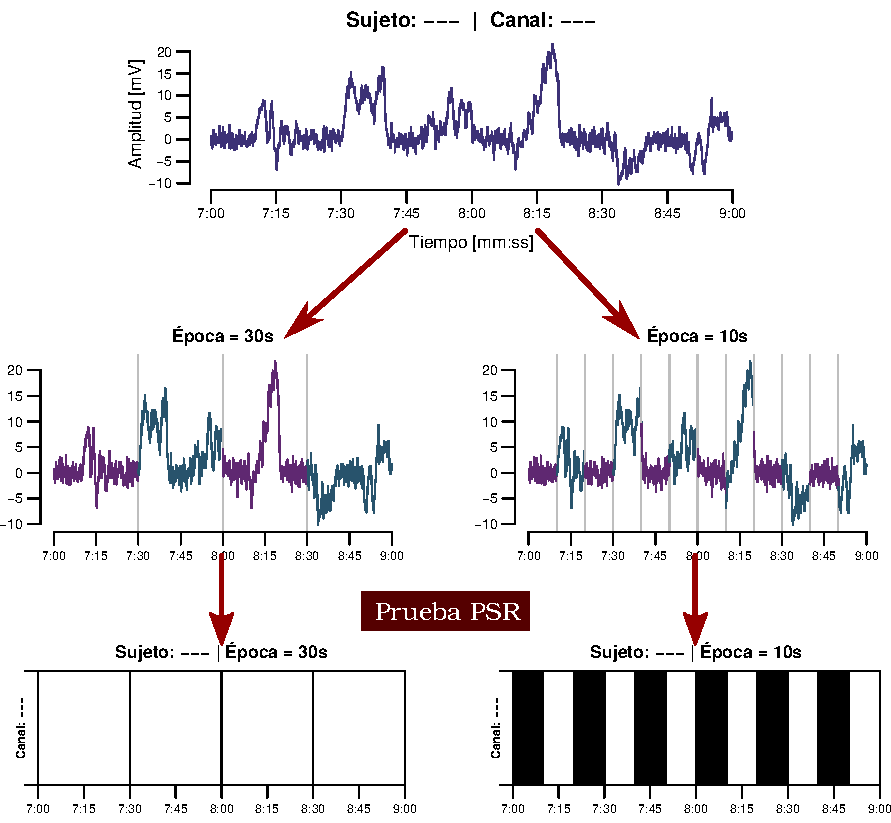
\includegraphics[width=\linewidth]{./img_diagramas/epocas_diferentes_v2.pdf}
\caption{Esquema de cómo se tomaron diferentes tamaños de época para estudiar los registros de 
PSG}
\label{epocas_diferentes}
\end{figure}



%%%%%%%%%%%%%%%%%%%%%%%%%%%%%%%%%%%%%%%%%%%%%%%%%%%%%%%%%%%%%%%%%%%%%%%%%%%%%%%%%%%%%%%%%%%%%%%%%%%
%%%%%%%%%%%%%%%%%%%%%%%%%%%%%%%%%%%%%%%%%%%%%%%%%%%%%%%%%%%%%%%%%%%%%%%%%%%%%%%%%%%%%%%%%%%%%%%%%%%
%%%%%%%%%%%%%%%%%%%%%%%%%%%%%%%%%%%%%%%%%%%%%%%%%%%%%%%%%%%%%%%%%%%%%%%%%%%%%%%%%%%%%%%%%%%%%%%%%%%
%%%%%%%%%%%%%%%%%%%%%%%%%%%%%%%%%%%%%%%%%%%%%%%%%%%%%%%%%%%%%%%%%%%%%%%%%%%%%%%%%%%%%%%%%%%%%%%%%%%

%%%%%%%%%%%%%%%%%%%%%%%%%%%%%%%%%%%%%%%%%%%%%%%%%%%%%%%%%%%%%%%%%%%%%%%%%%%%%%%%%%%%%%%%%%%%%%%%%%%
%%%%%%%%%%%%%%%%%%%%%%%%%%%%%%%%%%%%%%%%%%%%%%%%%%%%%%%%%%%%%%%%%%%%%%%%%%%%%%%%%%%%%%%%%%%%%%%%%%%
%%%%%%%%%%%%%%%%%%%%%%%%%%%%%%%%%%%%%%%%%%%%%%%%%%%%%%%%%%%%%%%%%%%%%%%%%%%%%%%%%%%%%%%%%%%%%%%%%%%
%%%%%%%%%%%%%%%%%%%%%%%%%%%%%%%%%%%%%%%%%%%%%%%%%%%%%%%%%%%%%%%%%%%%%%%%%%%%%%%%%%%%%%%%%%%%%%%%%%%

\chapter{Metodolog\'ia}

%El presente trabajo se llev\'o a cabo \textit{a posteriori}, usando los datos obtenidos en un 
%estudio previo \cite[V\'azquez Tagle, 2016]{VazquezTagle16}; 
%se espera que los resultados encontrados sean una
%extensi\'on de los resultados hallados previamente. 
En esta secci\'on se cita la metodolog\'ia 
manejada en \cite{VazquezTagle16}, 
siendo que el presente trabajo es una extensi\'on de aquel y que parte de los registros obtenidos;
debido a que la naturaleza y origen de estos datos es crucial para el trabajo presente, se trata de
presentar la metodolog\'ia original de la manera m\'as fiel posible.
%, por respeto a los autores y debido a su relevancia en el 
%reciente ana\'alisis sobre los mismos datos. 
Posteriormente se describen los an\'alisis realizados
sobre los datos, a nivel de implementaci\'on, usando el software estad\'istico R
y el paquete \texttt{fractal} \cite{R_citar,R_fractal};
las bases de estos an\'alisis se exponene en secciones anteriores.

En la primera etapa del tarbajo de \cite{VazquezTagle16},
los individuos se sometieron voluntariamente a una bater\'ia de pruebas
neuropsicol\'ogicas para diagnosticar PDC y depresi\'on geri\'atrica (ver m\'as adelante), 
que a su vez fungieron como criterios de
inclusi\'on para una segunda fase del estudio.
En el presente trabajo se han analizado sujetos que fueron excluidos de la segunda etapa de aqu\'el
trabajo, pero que accedieron a participar en la misma; esto se ha hecho con el fin de
verificar si los datos recabados justifican esta restricci\'on en futuros estudios.

En la etapa posterior, los individuos se sometieron voluntariamente a un estudio de la
actividad el\'ectrica cerebral durante el
sue\~no; se realizaron
registros de EEG en 22 sitios de muestreo, adicionalmente se midi\'o
actividad ocular y muscular a trav\'es de EOG y EMG --respectivamente-- con
el fin de detectar adecuadamente las etapas cl\'inicas del sue\~no\cite{AASM07}.
El registro simult\'aneo de estas se\~nales durante el sue\~no recibe el nombre de PSG.

%%%%%%%%%%%%%%%%%%%%%%%%%%%%%%%%%%%%%%%%%%%%%%%%%%%%%%%%%%%%%%%%%%%%%%%%%%%%%%%%%%%%%%%%%%%%%%%%%%%

\section{Pruebas sobre deterioro cognitivo}

La calidad de 'deterioro cognitivo' y 'depresi\'on geri\'atrica' en los participantes fue
determinada a partir de la aplicaci\'on de una pila de pruebas neuropsicol\'ogicas, que se
listan a continuaci\'on.

\begin{itemize}

\item {Evaluaci\'on Neuropsicol\'ogica (Neuropsi)} \cite{Solis03}
%El esquema está constituido por reactivos sencillos y cortos. 
%En la medida de lo posible se incluyeron pruebas con alta validez neuropsicológica y/o se 
%adaptaron estas pruebas para poder evaluar poblaciones de ancianos o psiqui\'atricas. 
%Las \'areas cognoscitivas que eval\'ua 
%el instrumento son 
%\begin{itemize}
%\item[I.] Orientaci\'on
%\item[II.] Atenci\'on y concentraci\'on
%\begin{itemize}
%\item[(a)] Deficiencias en el nivel de conciencia o estado de activaci\'on
%\item[(b)] Atenci\'on selectiva
%\item[(c)] Atenci\'on sostenida
%\item[(d)] Control atencional
%\end{itemize}
%\item[III.] Memoria
%\begin{itemize}
%\item[(a)] Memoria sensorial
%\item[(b)] Memoria a corto plazo
%\item[(c)] Memoria a largo plazo
%\item[(d)] Memoria de trabajo
%\end{itemize}
%\end{itemize}

\item {Mini Mental State Examination (MMSE)} 
%Creado en 1975 como instrumento para 
%la evaluación breve del estado mental, es el test m\'as utilizado para la evaluación cognitiva 
%estandarizada en el \'ambito cl\'inico, sobre todo en el anciano. Es el que dispone de m\'as 
%datos para el cribado, estadiaje y seguimiento de las demencias. As\'i mismo permite detectar 
%alteraciones cognitivas sutiles en pacientes con demencia incipiente o alteraci\'on cognitiva 
%leve, adem\'as de establecer un perfil cognitivo de los diferentes subtipos de 
%demencias.
\cite{Velasco15}

\item {Escala breve para la detecci\'on de ansiedad del anciano (SATS)} 
%Es un instrumento 
%que 
%consta de 10 preguntas espec\'ificas sobre malestar psicol\'ogico que se refieren a los 
%s\'intomas de ansiedad que puede tener una persona durante las cuatro semanas previas a la 
%aplicaci\'on. Las opciones de respuesta de las preguntas son tipo Likert, categorizadas en una 
%escala ordinal de cinco niveles: siempre, casi siempre, a veces, casi nunca y nunca. 
%A la respuesta \textit{nunca} se le asigna el valor escalar de 1 y a la respuesta 
%\textit{siempre}, de 5 puntos. La suma de las puntaciones tiene un m\'inimo de 10 y un máximo de 
%50. Los rangos del instrumento presentan cuatro niveles: bajo (10–15), moderado (16–21), 
%alto (22–29), y muy alto (30–50). La consistencia interna del instrumento fue de $\alpha$=0.90
\cite{Vargas11}

\item {Escala sobre las actividades cotidianas de la vida diaria (KATZ)} 
%Eval\'ua el nivel
%de independencia de las actividades de la vida diaria en pacientes con deterioro cognoscitivo y 
%demencia. Su aplicaci\'on es de alrededor de diez a quince minutos y no requiere de capacitaci\'on 
%previa. Consta de una primera parte donde se consignan los datos del paciente y del informante, 
%lugar, fecha y nombre del evaluador. Una segunda parte, est\'a formada por nueve \'items que se 
%corresponden con las actividades de la vida diaria b\'asicas (continencia urinaria, continencia 
%fecal, aseo, toilette, alimentaci\'on, movilidad, traslado dentro y fuera del hogar, ba\~no y 
%vestido), a su vez cada una de ellas est\'a desglosada en las acciones que conforman la tarea y la 
%forma en que el paciente la lleva a cabo. A cada actividad le corresponde un puntaje parcial, que 
%refleja la capacidad funcional del paciente. Se debe tener en cuenta que el \'item se corresponde 
%con el nivel \'optimo de funcionamiento y le corresponde el puntaje m\'as alto dentro de la escala,
%6 puntos. La suma de todos los resultados sirve para arribar a un puntaje total, que se 
%correlaciona con uno de los siete niveles de desempe\~no, determinando cu\'ando una persona 
%requiere indicaci\'on, supervisi\'on o asistencia f\'isica/verbal de otra para ejecutar todos los 
%pasos de una actividad. El puntaje total es 60 puntos, que corresponde al desempe\~no 
%independiente.
\cite{Roumec14}

\item {Escala de Depresi\'on Geri\'atrica (Gds)} 
%Esta escala ha sido probada y usada 
%extensamente 
%en la población adulta mayor. Con la escala Gds se valora la depresión en el adulto mayor que 
%puede confundirse con el deterioro cognitivo. Es conocido que la depresi\'on puede disparar el 
%deterioro f\'isico, cognitivo y social particularmente en el adulto 
%mayor. 
\cite{Greenberg12,Cuijpers13}

\end{itemize}

%%%%%%%%%%%%%%%%%%%%%%%%%%%%%%%%%%%%%%%%%%%%%%%%%%%%%%%%%%%%%%%%%%%%%%%%%%%%%%%%%%%%%%%%%%%%%%%%%%%

\section{Participantes}

En el trabajo original,
la muestra se eligi\'o de una manera no probabilística de sujetos tipo \cite{Garcia09}. De aquellos
s\'olo se han considerado 11 sujetos que accedieron a la segunda fase del estudio (obtenci\'on
de registros de PSG), que en conjunto conforman una muestra no necesariamente respresentativa de
la muestra total.

Usando los reultados de la bater\'ia de pruebas neuropsicol\'ogicas, los sujetos se dividieron
en tres grupos seg\'un los siguientes criterios
\begin{description}
\item[Grupo PDC] Adultos Mayores sin depresi\'on geri\'atrica %(puntuaci\''on Gds baja) 
ni enfermedades ''graves'' [preguntar t\'ermino exacto],
y cuya puntuaci\'on en Neuropsi fuera menor a 3 desviaciones est\'andar la repotada para poblaciones
control \cite{Solis03}
\item[Grupo control] Adultos Mayores sin depresi\'on geri\'atrica ni enfermedades ''graves'',
que no fueran considerados en el Grupo PDC
\item[Sujetos exclu\'idos] Sujetos que no cumplen los requerimientos para ser clasificados dentro de
los dos primeros grupos, pero que se sometieron voluntariamente al estudio
\end{description}
Con respecto al tercer grupo, se le prest\'o atenci\'on a modo de interpretar las capacidades y
limitaciones de las t\'ecnicas utilizadas; muchos estad\'isticos no ser\'an calculados para este
grupo,
%ya que no forman una unidad propiamente dicha, 
sino que se autoriz\'o su utilizaci\'on
para ejemplificar la validez de las restricciones para los sujetos de estudio. El sujeto 
FGH fue retirado debido a que padece par\'alisis facial y posiblemente da\~no cerebral; el sujeto MGG
fue retirado ya que padece depresi\'on geri\'atrica; el sujeto EMT fue retirado debido a que no
califica como Adulto Mayor por su edad.

%PDC, Normal y Extra (aquellos no considerados en el estudio original). En la tabla
%\ref{tab_sujetos} se han concentrado estos resultados.

%\begin{tabular}{l|ccc|ccccc|c}
%%\hline 
%%Nombre & Sexo & Edad & Esc. & Neuropsi & MMSE & SATS & KATZ & Gds & Notas \\
%\textbf{Nombre} & \textbf{Sexo} & \textbf{Edad} & \textbf{Esc.} & \textbf{Neuropsi} & \textbf{MMSE} & \textbf{SATS} & \textbf{KATZ} & \textbf{Gds} & \textbf{Notas} \\
%\hline 
%VCR    & F    & 59   & 12   & 107      & 29   & 21   & 0    & 3 & \\
%MJH    & F    & 72   & 9    & 113      & 30   & 18   & 0    & 0 & \\
%JAE    & F    & 78   & 5    & 102      & 28   & 19   & 0    & 5 & \\
%GHA    & M    & 65   & 9    & 107.5    & 30   & 23   & 0    & 7 & Disminuci\'on aguda visual y auditiva, alcoholismo previo \\
%MFGR   & F    & 67   & 11   & 110      & 30   & 18   & 0  &  \\
%\hline 
%CLO    & F    & 68   & 5    & 81       & 28 & 22 & 1 & 6 &  \\
%RLO    & F    & 63   & 9    & 90       & 29 & 20 & 0 & 3 &  \\
%RRU    & M    & 69   & 9    & 85       & 27 & 10 & 0 & 3 &  \\
%JGZ    & M    & 65   & 11   & 87       & 25 & 20 & 0 & 1 &  \\
%\hline 
%FGH    & M    & 71   & 9    & 83.5     & 21 & 23 & 0 & 4  &  Par\'alisis facial, hipotiroides, columna, cataratas  \\
%MGG    & F    & 61   & 9    & 114      & 28 & 29 & 1 & 14 &  \\
%EMT    & M    & 50   & 22   & 106      & 30 & 15 & 0 & 4  &  \\
%%\hline 
%\end{tabular} 

\begin{table}
\centering
\begin{tabular}{c}
\textbf{Datos generales de los participantes}
\vspace{1em}
\end{tabular}
\begin{small}
\begin{tabular}{c|ccc|ccccc}
%\hline 
%Nombre & Sexo & Edad & Esc. & Neuropsi & MMSE & SATS & KATZ & Gds & Notas \\
\textbf{Nombre} & \textbf{Sexo} & \textbf{Edad} & \textbf{Esc.} & \textbf{Neuropsi} & \textbf{MMSE} & \textbf{SATS} & \textbf{KATZ} & \textbf{Gds} \\
\hline 
\hline 
VCR    & F    & 59   & 12   & 107      & 29   & 21   & 0    & 3 \\
MJH    & F    & 72   & 9    & 113      & 30   & 18   & 0    & 0 \\
JAE    & F    & 78   & 5    & 102      & 28   & 19   & 0    & 5 \\
GHA    & M    & 65   & 9    & 107.5    & 30   & 23   & 0    & 7 \\
MFGR   & F    & 67   & 11   & 110      & 30   & 18   & 0    &   \\
\hline 
$\widehat{\mu}$ & 
              & 68.20& 9.20 & 107.90   & 29.40& 19.80& 0.00 & 3.00\\
$\widehat{\sigma}$ & 
              & 7.19 & 2.68 & 4.07     & 0.89 & 2.17 & 0.00 & 3.08\\
\hline 
\hline 
CLO    & F    & 68   & 5    & 81       & 28   & 22   & 1    & 6 \\
RLO    & F    & 63   & 9    & 90       & 29   & 20   & 0    & 3 \\
RRU    & M    & 69   & 9    & 85       & 27   & 10   & 0    & 3 \\
JGZ    & M    & 65   & 11   & 87       & 25   & 20   & 0    & 1 \\
\hline 
$\widehat{\mu}$ & 
              & 66.25& 8.50 & 85.75   & 27.25& 18.00& 0.25 & 3.25\\
$\widehat{\sigma}$ & 
              & 2.75 & 2.52 & 3.77    & 1.71 & 5.42 & 0.50 & 2.06\\
\hline 
\hline 
FGH    & M    & 71   & 9    & 83.5     & 21   & 23   & 0    & 4  \\
MGG    & F    & 61   & 9    & 114      & 28   & 29   & 1    & 14 \\
EMT    & M    & 50   & 22   & 106      & 30   & 15   & 0    & 4  \\
%\hline 
\end{tabular} 
\end{small}
\label{tab_sujetos}
\caption{Resultados de las pruebas neuropsicol\'ogicas aplicadas a los sujetos considerados
en este trabajo, adem\'as de algunos datos generales de estos mismos sujetos. \textbf{Notas:}
\underline{GHA:} Disminuci\'on aguda visual y auditiva, alcoholismo previo. 
\underline{FGH:} Par\'alisis facial, hipotiroides, columna, cataratas.}
\end{table}

Cabe mencionar que, aunque se aplic\'o la bater\'ia entera de test neuropsicol\'ogicos mencionados
anteriormente, se ha valorado fuertemente el resultado de Neuropsi dentro del diagn\'ostico de PDC
como conclusi\'on del trabajo original \cite{VazquezTagle16}.
Se han inclu\'ido los resultados de la bater\'ia completa de test con el fin de citarla en la
discusi\'on, ya que cada uno se 'especializa' en aspectos particulares --atenci\'on, memoria a corto
y largo plazo, memoria declarativa y de trabajo, etc; si bien no se profundizar\'a en estos
conceptos, no puede omitirse el hecho que estas actividades espec\'ificas se consideran
localizadas --de manera muy general-- en \'areas espec\'ificas del cerebro.

%Es indipensable aclarar que,
%En el protocolo 
Para la obtenci\'on de estos datos,
%en \cite{VazquezTagle16} 
%se declara la participaci\'on informada 
los participantes declararon su participaci\'on libre e informada en el estudio
%y libre de los sujetos 
bajo los siguientes t\'erminos \cite{VazquezTagle16}:
\begin{quote}
La participaci\'on en el estudio es completamente 
voluntaria, pudiendo los sujetos abandonar las intervenciones en cualquier momento. Todos los 
participantes firmaron un consentimiento informado previamente a su inclusi\'on en el estudio. 
Los protocolos experimentales empleados en esta investigaci\'on fueron previamente aprobados por 
el Comit\'e \'Etico de Investigaci\'on en humanos de la Universidad Autónoma del Estado de Hidalgo.
%La muestra se eligi\'o de una manera no probabilística de sujetos tipo \cite{Garcia09}.
\end{quote}

%%%%%%%%%%%%%%%%%%%%%%%%%%%%%%%%%%%%%%%%%%%%%%%%%%%%%%%%%%%%%%%%%%%%%%%%%%%%%%%%%%%%%%%%%%%%%%%%%%%

\section{Electroencefal\'ografo utilizado}

Para registrar el PSG se ha usado 
{electroencefal\'ografo digital MEDICID 5.} 
(Neuronic mexicana S.A. de C.V.)
% MEDICID. MEDICID 5. 2016; : 1.]
%Es un electroencefal\'ografo digital de 
%cuenta con
%32 canales, 24 de ellos monopolares con posibilidades de 
%programaci\'on y 8 bipolares con la posibilidad de conexi\'on monopolar para conformar 32 canales 
%con referencia com\'un. 
%Esto hace posible preparar por software los montajes que comunmente son 
%conocidos en los equipos tradicionales de poligraf\'ia en papel. 
%Los amplificadores bipolares son 
%especialmente dise\~nados para la conexi\'on sensorial o la transducci\'on de la medici\'on por 
%signos biof\'isicos, (esfuerzo respiratorio abdominal y tor\'acico, flujo a\'ereo nasal y bucal) 
%cuando los registros poligr\'aficos est\'an hechos. 
%%%Con el MEDICID se pueden usar las siguientes aplicaciones: 
%%%\begin{itemize}
%%%\item \underline{Trackwalker.} Sistema b\'asico de electroencefalograf\'ia digital con EEG 
%%%cuantitativo y mapeo cerebral.
%%%
%%%\item \underline{Dream Hunter.} Sistema para estudios del sue\~no.
%%%
%%%\item \underline{Mind Tracer.} Sistema para el estudio de Potenciales Evocados 
%%%relacionados a eventos.
%%%
%%%\item \underline{EP Workstation.} Sistema para la estimaci\'on y el an\'alisis de los 
%%%Potenciales Relacionados a Eventos (PRE) end\'ogenos de alta densidad (128 canales). 
%%%\end{itemize}
Especificaciones T\'ecnicas:
\begin{itemize}
\item 24 canales monopolares (0.05 -- 100 Hz)
\item 8 canales bipolares para poligraf\'ia (0.5 -- 100 Hz)
\item 3 canales de C.C. (0--160 Hz)
\item 1 canal de temperatura (30 -- 40 C)
\item 1 estimulador f\'otico (0.5 -- 33 Hz)
\item Sistema A/D: 16 bits
\item Frec. Muestreo: Hasta 500 Hz (36 canales)
\item Voltaje Alimentaci\'on: 100 -- 240 V, 50/60 Hz
\item Interfaz: USB
\item Dimensiones: Bloque de control: ($257 \times 315 \times 55$ mm)
\item Peso: Bloque de control: 2.5 kg
\item Bloque amplificadores: ($110\times 187\times 50$ mm)
\item Bloque amplificadores: 1.0 kg
\item Seguridad el\'ectrica: Clase I Tipo BF (Certificado según EN60601-1)
\end{itemize}

%%%%%%%%%%%%%%%%%%%%%%%%%%%%%%%%%%%%%%%%%%%%%%%%%%%%%%%%%%%%%%%%%%%%%%%%%%%%%%%%%%%%%%%%%%%%%%%%%%%

\section{Registro del polisomnograma}

Una vez aplicada
%el Neuropsi y toda 
la bater\'ia de pruebas ya mencionada, los adultos mayores
participantes fueron invitados a acudir a las instalaciones de la Cl\'inica Gerontol\'ogica de 
Sue\~no, ubicada en las instalaciones del Instituto de Ciencias de la Salud de la Universidad 
Aut\'onoma del Estado de Hidalgo.

Los participantes recibieron instrucciones de realizar una rutina normal de actividades durante la 
semana que precedi\'o al estudio. Tambi\'en se les recomend\'o que no ingirieran bebidas 
alcoh\'olicas o energizantes como caf\'e o refrescos durante las 24 horas previas al experimento, 
ni durmieran siesta el d\'ia del estudio. 

%Cada participante lleg\'o a las instalaciones alrededor de las 17:00 hrs. para la colocaci\'on de 
%los electrodos, ya que este procedimiento tarda de entre 2 a 3 horas. La hora de comienzo del 
%registro de PSG fue adaptado a la hora habitual de acostarse de cada sujeto.

El protocolo de PSG incluye 19 electrodos de EEG,
%\begin{itemize}
%\item Fp1 
%\item Fp2
%\item AF7
%\item AF3
%\item AFz
%\item AF4
%\item AF8
%%\item F7
%\item F5
%%\item F3
%\item F1
%%\item Fz
%\item F2
%%\item F4
%\item F6
%%\item F8
%\item FT7 
%\item FC5
%\item FC3
%\item FC1
%\item FCz
%\item FC2
%\item FC4
%\item FC6
%\item FT8
%%\item T7
%%\item C5
%%\item C3
%%\item C1
%%\item Cz
%%\item C2
%%\item C4
%%\item C6
%%\item T8
%\item TP7
%\item CP5
%\item CP3
%\item CP1
%\item CPz
%\item CP2
%\item CP4
%\item CP6
%\item TP8
%%\item P7
%%\item P5
%%\item P3
%%\item P1
%%\item Pz
%%\item P2
%%\item P4
%%\item P6
%%\item P8
%\item PO7
%\item PO3
%\item POz
%\item PO4
%\item PO8
%\item O1
%\item O2
%\end{itemize}
4 electrodos de EOG para registrar movimientos oculares horizontales y verticales, 
y 2 electrodos de EMG colocados en los m\'usculos submentonianos para registrar la actividad 
muscular. 
La colocaci\'on de los electrodos para registrar la actividad EEG se realiz\'o siguiendo las 
coordenadas del Sistema Internacional 10-20\cite{Coleman87}.

%%\begin{figure}
%%\centering
%%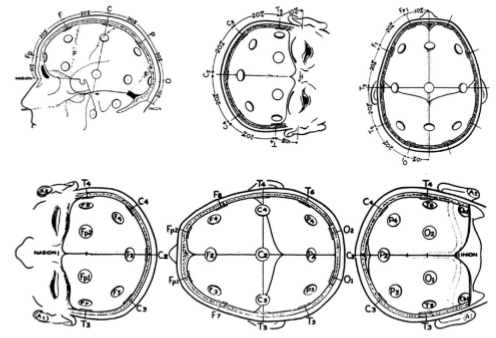
\includegraphics[width=\linewidth]{figura_6.png} 
%%\caption{El sistema 10--20, recomendado por la
%%International Federation of EEG Societies. 
%%%\cite{Jasper58,AASM07}
%%}
%%%\label{img1020}
%%\end{figure}

%Previamente a la colocaci\'on de cada electrodo, se frot\'o la zona de inter\'es con un algod\'on 
%empapado en crema abrasiva con el objetivo de eliminar las c\'elulas muertas y la grasa de la piel.
%Posteriormente, la copa de cada electrodo se rellen\'o con una pasta electrol\'itica 
%conductora (Ten20\texttrademark, Weaver) para mejorar la conductividad  entre la piel y el 
%electrodo. Los electrodos para registrar el EEG se fijaron al cuero cabelludo con colodi\'on 
%(solución al 4\%, Panreac), mientras que los electrodos de poligraf\'ia (EOG y EMG) fueron 
%adheridos a la piel de la cara con cinta quir\'urgica extra-adhesiva (Cinta 
%Micropore\texttrademark). Para acelerar el proceso de fijaci\'on y secado del colodi\'on, se 
%aplic\'o aire comprimido a cada electrodo colocado sobre el cuero cabelludo.

Las se\~nales electrofisiol\'ogicas de cada registro PSG fueron amplificadas, filtradas y 
digitalizadas %con el programa para ordenador \texttt{Registro de sue\~no} 
para su posterior interpretaci\'on. 
%El registro se llev\'o a cabo con una tasa de muestreo de 512 Hz o 200 Hz (puntos por segundo)
%seg\'un la disponibilidad del electroencefal\'ografo.
Debido a problemas t\'ecnicos con el electroencefal\'ografo, el registro se llev\'o a cabo
a 512 Hz para algunos sujetos y a 200 Hz para otros; en la tabla \ref{frecuencias}
se presenta tal informaci\'on.

%\begin{table}
%\begin{tabular}{c|cc}
%Sujeto & Frec. de muestreo \\
%& 512 & 200 \\
%\hline
%\hline
%VCR & & * \\
%MJH & * & \\ 
%JAE & * & \\
%GHA &  & * \\
%MFGR &  & * \\
%CLO & * & \\
%RLO & * & \\
%RRU &  & * \\
%JGZ &  & * \\
%\hline
%FGH & * & \\
%MGG &  & * \\
%EMT &  & * \\
%\end{tabular}
%\label{frecuencias}
%\end{table}

\begin{table}
\centering
\begin{tabular}{c}
\textbf{Datos generales sobre los registros de PSG}
\vspace{1em}
\end{tabular}
\begin{tabular}{c||c|cc|ccc}
    &Frecuencia& \underline{Total}& &   &\underline{MOR} &         \\
    &muestreo  &Puntos  &  Tiempo   &Puntos  &  Tiempo   &  \% MOR \\
\hline
\hline
VCR &200       & 5166000&   7:10:30 &438000  &   0:36:30 & 8\% \\
MJH &512       &15851520&   8:36:00 &1950720 &   1:03:30 &12\% \\
JAE &512       &13931520&   7:33:30 &2626560 &   1:25:30 &19\% \\
GHA &200       &6558000 &   9:06:00 &330000  &   0:27:30 & 5\% \\
MFGR&200       &4932000 &   6:51:00 &570000  &   0:47:30 &12\% \\
\hline
CLO &512       &14499840&   7:52:00 &2027520 &   1:06:00 &14\% \\
RLO &512       &12994560&   7:03:00 &1520640 &   0:49:30 &12\% \\
RRU &200       &2484000 &   3:27:00 &228000  &   0:19:00 & 9\% \\
JGZ &512       &18539520&  10:03:30 &506880  &   0:16:30 & 3\% \\
\hline
FGH &512       &6220800 &   3:22:30 &337920  &   0:11:00 & 5\% \\
MGG &512       &15820800&   8:35:00 &2549760 &   1:23:00 &16\% \\
EMT &512       &21857280&  11:51:30 &721920  &   0:23:30 & 3\%
\end{tabular}
\caption{Cantidad de datos analizados para cada sujeto. Debido a un cambio en el
polisomn\'ografo usado, la frecuencia de muestreo --en Hz-- cambia entre sujetos; la recomendaci\'on 
de la AASM, un m\'inimo de 128 Hz, se cumple.
%Debido a que que los registros fueron segmentados en \'epocas de 30 segundos,
%algunos datos al final de los registros fueron deshechados. 
El sue\~no MOR aparece fragmentado, se reporta la suma de esos tiempos.}
\label{frecuencias}
%\end{SidewaysFigure}
\end{table}

\begin{figure}
\centering
\subfloat{
\includegraphics[width=\linewidth]
%{./material170327/grafiquitos170327/MJH_190_PDG.pdf} 
{./p_170427/MJH_190_PDG_lucirse_PSG.pdf}
}\\
\subfloat{
\includegraphics[width=\linewidth]
%{./material170327/grafiquitos170327/JGZ_375_PDG.pdf} 
{./p_170427/JGZ_367_PDG_lucirse_PSG.pdf}
}\\
\caption{Ejemplos de registros de PSG en sue\~no MOR para los sujetos MJH y JGZ.
N\'otense que el canal EMG permantece silente, mientras que
que los canales ROG y LOG exhiben actividad de gran amplitud y sincronizaci\'on (tanto como
iguales como reflejos).
Estas caracter\'isticas son resultado de patrones en base a los cuales se define
el sue\~no MOR:
%esta descripci\'on se ajusta a \textit{movimientos oculares r\'apidos}
%y \textit{aton\'ia muscular}
movimientos oculares r\'apidos y aton\'ia muscular.}
\label{ejemplos_mor}
\end{figure}

%\begin{figure}
%\centering
%\subfloat{
%\includegraphics[width=\linewidth]
%{./material170327/grafiquitos170327/MJH_281_PDG.pdf} 
%}\\
%\subfloat{
%\includegraphics[width=\linewidth]
%{./material170327/grafiquitos170327/JGZ_200_PDG.pdf} 
%}\\
%\caption{Ejemplos de registros de PSG en sue\~no no-MOR para los sujetos MJH y JGZ, para ser
%contrastados contra los registros en \ref{ejemplos_mor}.
%La actividad de LOG y ROG es m\'as ''peque\~na'' y desincronizada, mientras que la actividad de
%EMG es notoria, si bien no especialmente ''grande''.
%}
%\label{ejemplos_nmor}
%\end{figure}

%%%%%%%%%%%%%%%%%%%%%%%%%%%%%%%%%%%%%%%%%%%%%%%%%%%%%%%%%%%%%%%%%%%%%%%%%%%%%%%%%%%%%%%%%%%%%%%%%%%

\section{Clasificaci\'on de las etapas de sue\~no}

La clasificaci\'on de las diferentes fases del sue\~no en el registro PSG se realiz\'o manualmente 
sobre \'epocas de EEG de 30 segundos (filtro paso de banda de 0.5--30 Hz) siguiendo los criterios 
estandarizados de la AAIC\cite{Hori01}, que se exponen a continuación:
\begin{description}
\item[Vigilia (W)] Presencia de ritmo alfa contin\'uo con m\'axima amplitud 
sobre regiones de la corteza parieto-occipital. Tono muscular relativamente alto y ausencia de 
movimientos oculares.

\item[Fase 1 (N1)] %Transici\'on entre la vigilia y el sue\~no ligero. 
Presencia intermitente de 
actividad alfa en menos del 50\% de la \'epoca junto con movimientos oculares lentos y una ligera 
reducci\'on del tono muscular respecto al de vigilia.

\item[Fase 2 (N2)] Presencia de complejos K y husos de sue\~no. Puede aparecer hasta un 20\% de ondas 
lentas (ritmo delta, 0.5-3 Hz) en la \'epoca. Ausencia de actividad ocular y tono muscular bajo.

\item[Fase 3 (N3)] Presencia de ondas lentas con amplitudes superiores a 75 $\mu$V en m\'as del
20\% y menos del 50\% de la \'epoca. Pueden tambi\'en aparecer complejos K y husos de sue\~no de 
forma espor\'adica. Ausencia de actividad ocular y tono muscular bajo.

\item[Fase 4 (N4)] Presencia de ondas lentas en m\'as del 50\% de la época. Las dem\'as 
caracter\'isticas son similares a las de la fase 3.

\item[Fase MOR (R)] Presencia de actividad EEG de baja amplitud y frecuencias entremezcladas 
(theta-alfa-beta) similar a la observada en el estado de vigilia activa con ojos abiertos.
\end{description}

%%%%%%%%%%%%%%%%%%%%%%%%%%%%%%%%%%%%%%%%%%%%%%%%%%%%%%%%%%%%%%%%%%%%%%%%%%%%%%%%%%%%%%%%%%%%%%%%%%%

\section{Aplicaci\'on del test de Priestley-Subba Rao}

Para el an\'alisis de los registros de PSG se us\'o el software estad\'istico R\cite{R_citar}, 
as\'i como el paquete \texttt{fractal} \cite{R_fractal}.

Los registros digitalizados de PSG fueron convertidos a formato de texto (\texttt{.txt}) bajo
la codificaci\'on ASCII, a raz\'on de un archivo por cada canal. Posteriormente fueron importados
en el ambiente R y segmentados en sub-series de 30 segundos [10 segundos para algunos 
registros] acordes al concepto de \'epocas, y tomando en cuenta la tasa de muestreo de 512 [200]
puntos por segundo. 
En una primera etapa del trabajo solamente fueron incluidas sub-series correspondientes a
\'epocas de sue\~no MOR

%Como se mencion\'o en secciones anteriores, 
Dado que
el test PSR est\'a pensado para
series de tiempo con valor esperado constante 0, varianza finita en todo momento y espectro
continuo (ver secciones anteriores para m\'as detalles). Si bien la 
segunda condici\'on se 
ha supuesto satisfecha para el sistema en cuesti\'on
%satisface claramente en los sistemas biol\'ogicos [buscar respaldo
%para esta afirmaci\'on], la primera condici\'on no tiene por qu\'e cumplirse, 
las otras dos condiciones ser\'an ''forzadas'' aplicando  un
filtro que, idealmente, elimine la media y cualquier componente peri\'odica.
%esta separaci\'on es referida poopularmente como \textit{descomposici\'on cl\'asica}.
En este trabajo se usa el algoritmo no-param\'etrico Seasonal-Trend decomposition using Loess 
(STL), introducido por Clevelland et al. \cite{Cleveland1990} y que est\'a implementado en R.
%que permita separar el registro en una parte peri\'odica y una funci\'on
%de modo que es forzada usando el 
%filtro no-param\'etrico STL\cite{Cleveland1990} sobre cada una de las 
%sub-series\footnote{En la secci\'on de discusi\'on se abordar\'an las consecuencias de tal fitrado,
%mientras que en un anexo se describen los detalles en s\'i de este filtro.}.
Una justificaci\'on para hacer uso de este tipo de filtro es 
que no se espera estudiar la estructura de la se\~nal, sino si posee una caracter\'istica
que no ser\'a afectada por este filtro.

Con respecto al test PSR, sus detalles te\'oricos fueron discutidos en secciones anteriores.
%Los detalles te\'oricos del test PSR fueron discutidos con anterioridad. 
A modo
de resumen: se estima localmente el logaritmo del m\'odulo de la SDF
para algunos tiempos y frecuencias puntuales
%, para lo cual se usa un estimador
%local cuya varianza es conocida; 
posteriormente se procede a revisar
%, como prueba de
%hip\'otesis, 
si las cantidades obtenidas anteriormente son estad\'isticamente constantes
en el tiempo --como prueba de hip\'otesis.
El test PSR se encuentra implementado en R bajo la funci\'on \texttt{stationarity}
del paquete \texttt{fractal}; en la figura \ref{res_psr} puede verse la forma en que se
visualizan los resultados de esta funci\'on en la consola de R.

Los resultados del test PSR, aplicado a todas las \'epocas contenidas en los registros de PSG,
fueron almacenados para su an\'alisis posterior, mismo que se presenta m\'as adelante.

\begin{figure}
\centering
\begin{lstlisting}
Priestley-Subba Rao stationarity Test for datos
-----------------------------------------------
Samples used              : 3072 
Samples available         : 3069 
Sampling interval         : 1 
SDF estimator             : Multitaper 
  Number of (sine) tapers : 5 
  Centered                : TRUE 
  Recentered              : FALSE 
Number of blocks          : 11 
Block size                : 279 
Number of blocks          : 11 
p-value for T             : 0.4130131 
p-value for I+R           : 0.1787949 
p-value for T+I+R         : 0.1801353 
\end{lstlisting}
\caption{Resultado de una ejecuci\'on t\'ipica de la funci\'on \texttt{stationarity}
usando un vector de datos llamado \texttt{datos}. 
El n\'umero de bloques \texttt{n.blocks} define la cantidad de puntos en el tiempo
para los cuales se calcular\'a el estimador de la SDF
--se calcula por default como
$\max \left( 2 , \left\lfloor \log_2\left( N \right) \right\rfloor \right)$, donde
$N$ es la cantidad de datos en la serie.
%, aunque puede ingresarse un valor arbitrario.
Los filtros \textit{tapers} son usados para compensar el efecto de frecuencias m\'as altas que la 
tasa de muestreo, o de aquellas cuya longitud de onda sea mayor que la longitud de la serie;
para mayor informaci\'on vea secciones anteriores.
Cabe se\~nalar el antepen\'ultimo rengl\'on (\texttt{p-value for T}), que refleja el rechazo de 
%la prueba de 
hip\'otesis de estacionariedad d\'ebil --en el tiempo.}
\label{res_psr}
\end{figure}

%%%%%%%%%%%%%%%%%%%%%%%%%%%%%%%%%%%%%%%%%%%%%%%%%%%%%%%%%%%%%%%%%%%%%%%%%%%%%%%%%%%%%%%%%%%%%%%%%%%
%%%%%%%%%%%%%%%%%%%%%%%%%%%%%%%%%%%%%%%%%%%%%%%%%%%%%%%%%%%%%%%%%%%%%%%%%%%%%%%%%%%%%%%%%%%%%%%%%%%
%%%%%%%%%%%%%%%%%%%%%%%%%%%%%%%%%%%%%%%%%%%%%%%%%%%%%%%%%%%%%%%%%%%%%%%%%%%%%%%%%%%%%%%%%%%%%%%%%%%
%%%%%%%%%%%%%%%%%%%%%%%%%%%%%%%%%%%%%%%%%%%%%%%%%%%%%%%%%%%%%%%%%%%%%%%%%%%%%%%%%%%%%%%%%%%%%%%%%%%

%%%%%%%%%%%%%%%%%%%%%%%%%%%%%%%%%%%%%

%%%%%%%%%%%%%%%%%%%%%%%%%%%%%%%%%%%%%%%%%%%%%%%%%%%%%%%%%%%%%%%%%%%%%%%%%%%%%%%%%%%%%%%%%%%%%%%%%%%
%%%%%%%%%%%%%%%%%%%%%%%%%%%%%%%%%%%%%%%%%%%%%%%%%%%%%%%%%%%%%%%%%%%%%%%%%%%%%%%%%%%%%%%%%%%%%%%%%%%
%%%%%%%%%%%%%%%%%%%%%%%%%%%%%%%%%%%%%%%%%%%%%%%%%%%%%%%%%%%%%%%%%%%%%%%%%%%%%%%%%%%%%%%%%%%%%%%%%%%
%%%%%%%%%%%%%%%%%%%%%%%%%%%%%%%%%%%%%%%%%%%%%%%%%%%%%%%%%%%%%%%%%%%%%%%%%%%%%%%%%%%%%%%%%%%%%%%%%%%

\chapter{Resultados}

En cada canal que conforma el PSG (EEG, EOG y EMG), cada \'epoca registrada fue 
clasificada como 'posiblemente estacionaria' (PE) si, usando el test PSR
no pudo rechazarese la hip\'otesis de 
estacionariedad ($\alpha < 0.05$), o como 'no--estacionaria' en caso contrario.
%Variar el valor cr\'itico para esta clasificaci\'on no pareci\'o generar diferencias significativas.
La cantidad de \'epocas PE en cada individuo, durante el sue\~no MOR y NMOR, se muestra en las tablas 
\ref{total_gpos_mor}, \ref{total_gpos_nmor} y \ref{total_gpos_total}. Debido a la gran 
variabilidad entre los sujetos para la duraci\'on del sue\~no MOR, se consider\'o no 
el total de \'epocas PE sino la proporci\'on de \'estas en cada etapa de sue\~no; 
tales resultados se muestran en las tablas \ref{gpos_mor}, \ref{gpos_nmor} y \ref{gpos_total}. 
Adicionalmente se han calculado promedios y desviaciones est\'andar 
%grupales, seg\'un la
%clasificaci\'on arrojada por las pruebas neuropsicol\'ogicas.
para ambos grupos (Control y PDC)

Como un primer an\'alisis se verific\'o si el sue\~no MOR, entendido como muestra del registro
completo, tiene o no prpiedades estad\'sticas pareceidas a este \'ultimo --y si \'esta similaridad 
pudiera estar relacionada con el PDC. 
Se compar\'o la proporci\'on de \'epocas PE en cada canal durante sue\~no MOR y NMOR usando la 
prueba $\chi^{2}$ para proporciones\footnote{Implementada en R como la funci\'on 
\texttt{prop.test()}}; los resultados se muestran en la tabla \ref{comparacion_mor_vs_total},
aunque son resumidos esquem\'aticamente en la figura \ref{cabecitas_munchas}.

Se encontr\'o que no hay diferencias significativas, consistentes en todos los sujetos, en los 
canales LOG y ROG, lo cual puede ser explicado por la tipificaci\'on del sue\~no MOR. 
Por otro lado, no se encontr\'o una relaci\'on clara entre el estado de salud del sujeto y la 
aparici\'on de diferencias significativas entre estas proporciones.

\begin{figure}
\centering
\begin{tabular}{c}
\begin{tabular}{ccccc}
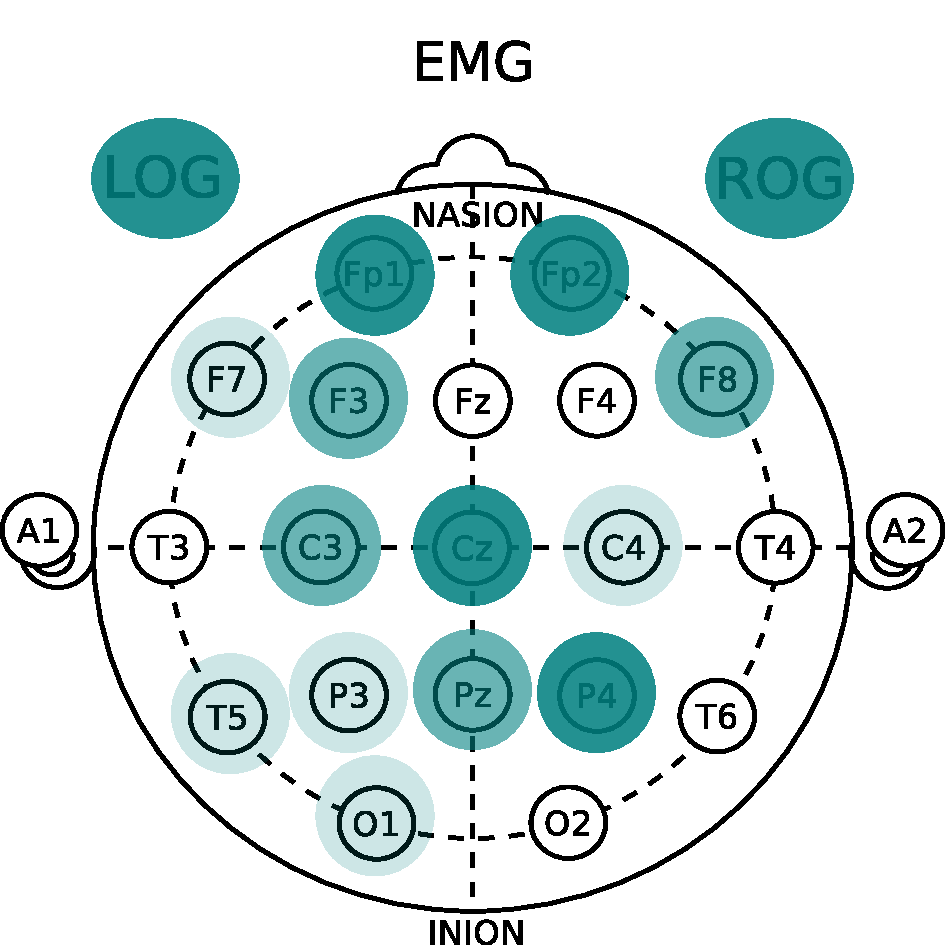
\includegraphics[width=0.17\textwidth]{./cabecitas/cabecita_VCR.pdf} &
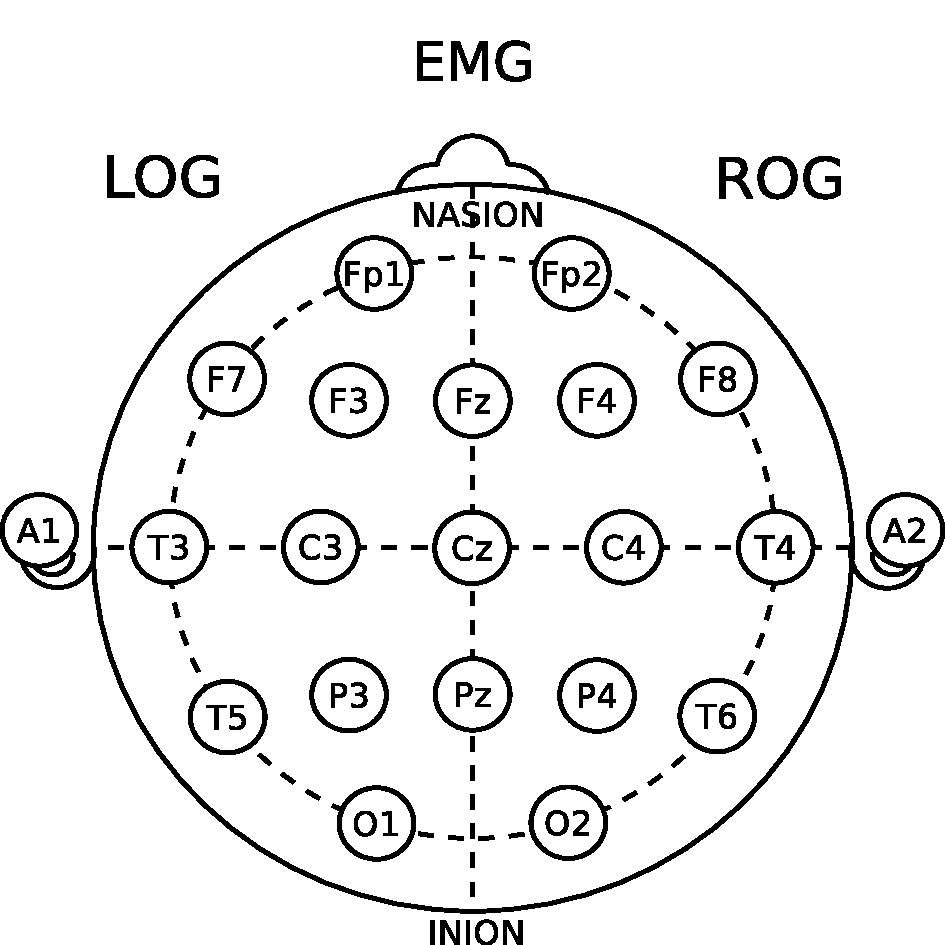
\includegraphics[width=0.17\textwidth]{./cabecitas/cabecita_MJH.pdf} &
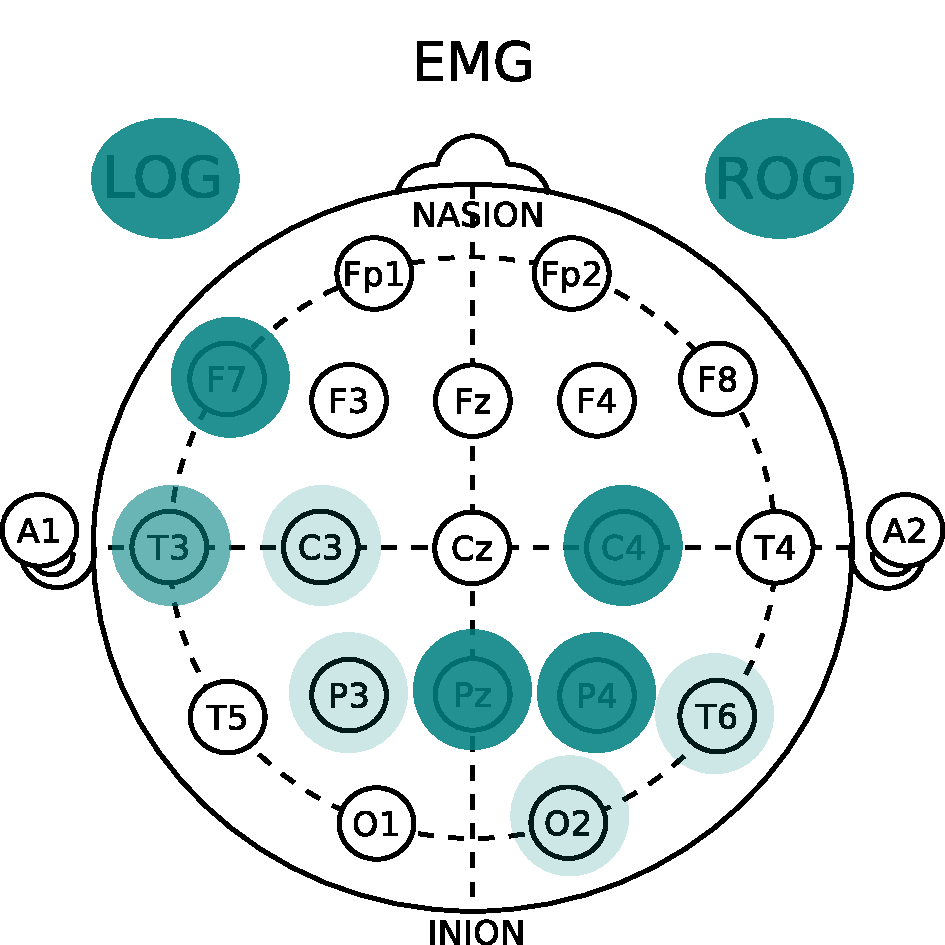
\includegraphics[width=0.17\textwidth]{./cabecitas/cabecita_JAE.pdf} &
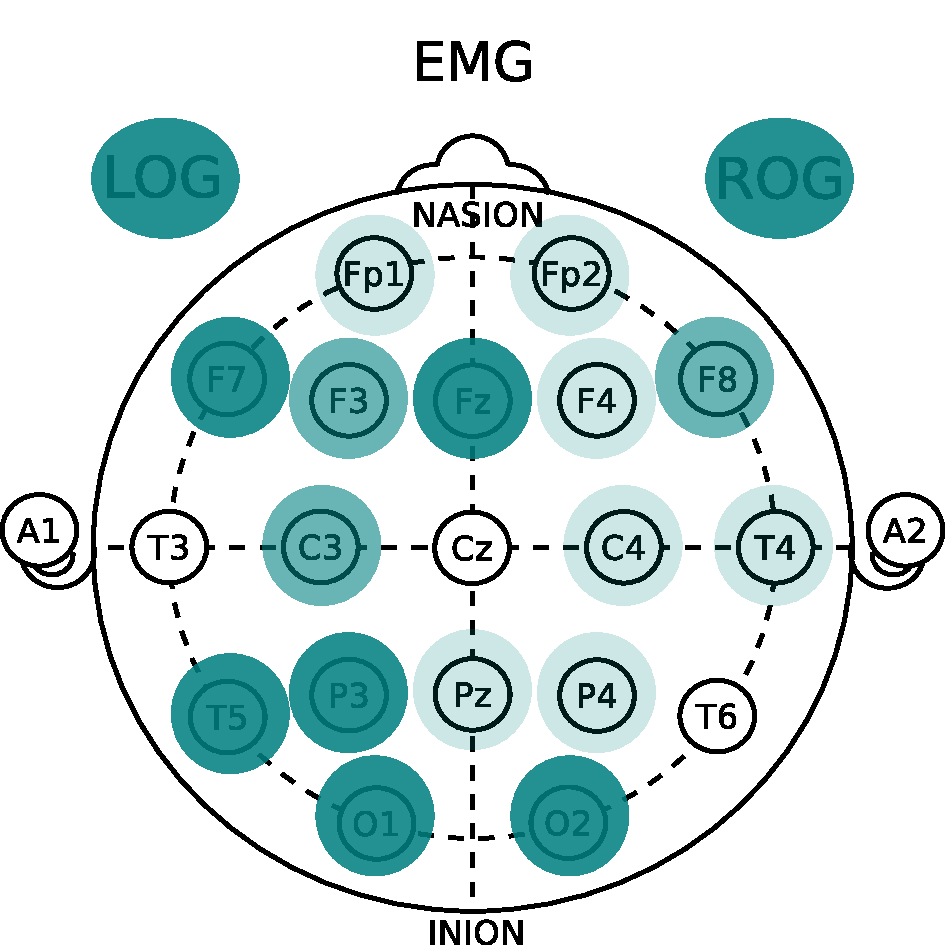
\includegraphics[width=0.17\textwidth]{./cabecitas/cabecita_GHA.pdf} &
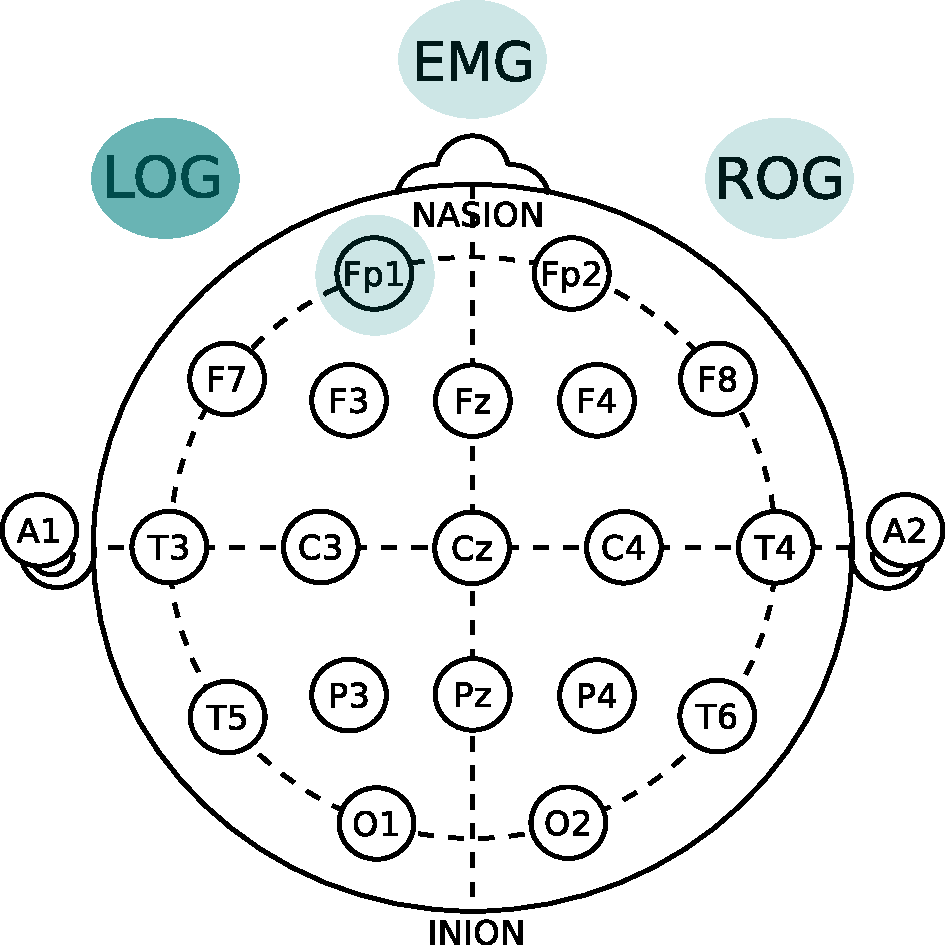
\includegraphics[width=0.17\textwidth]{./cabecitas/cabecita_MFGR.pdf} \\
VCR & MJH & JAE & GHA & MFGR
\end{tabular}
\\
\begin{tabular}{cccc}
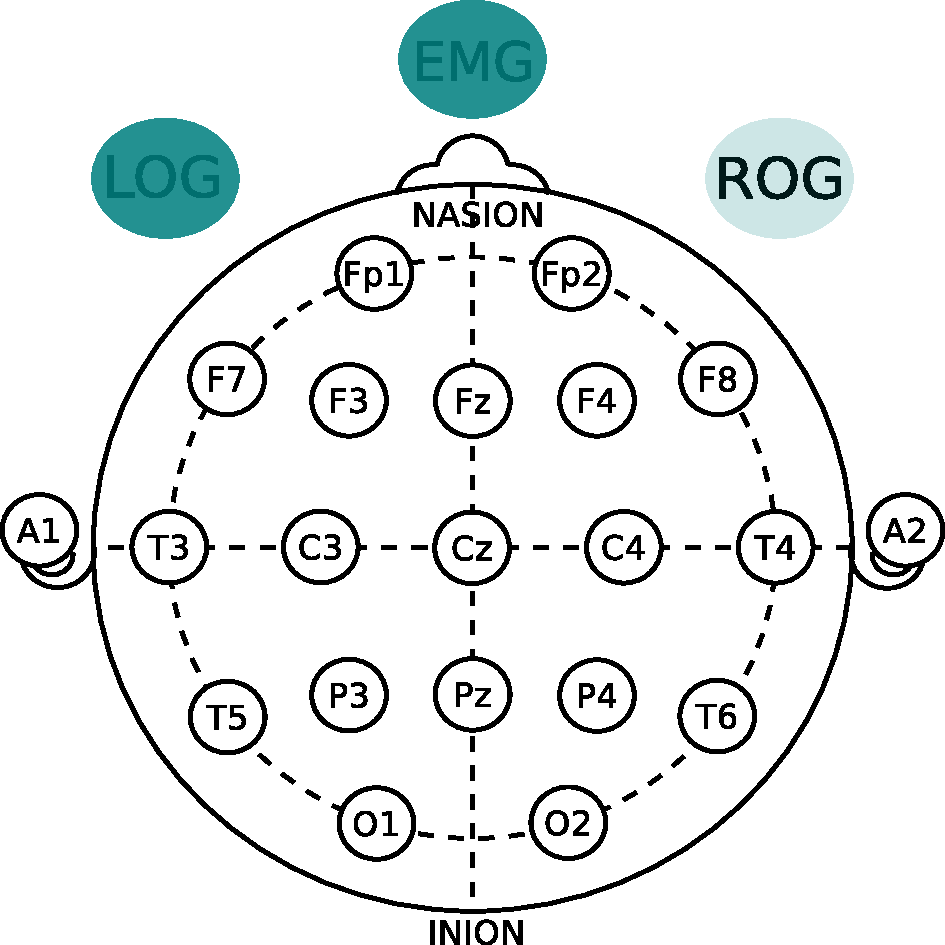
\includegraphics[width=0.17\textwidth]{./cabecitas/cabecita_CLO.pdf} &
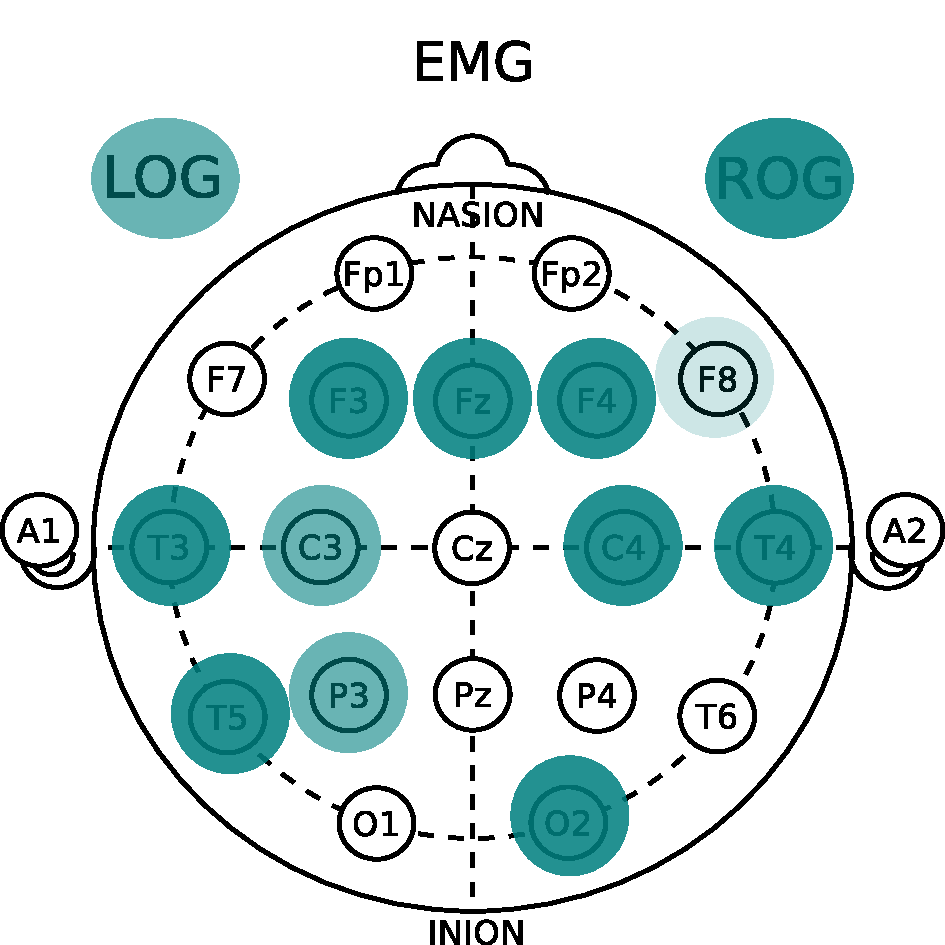
\includegraphics[width=0.17\textwidth]{./cabecitas/cabecita_RLO.pdf} &
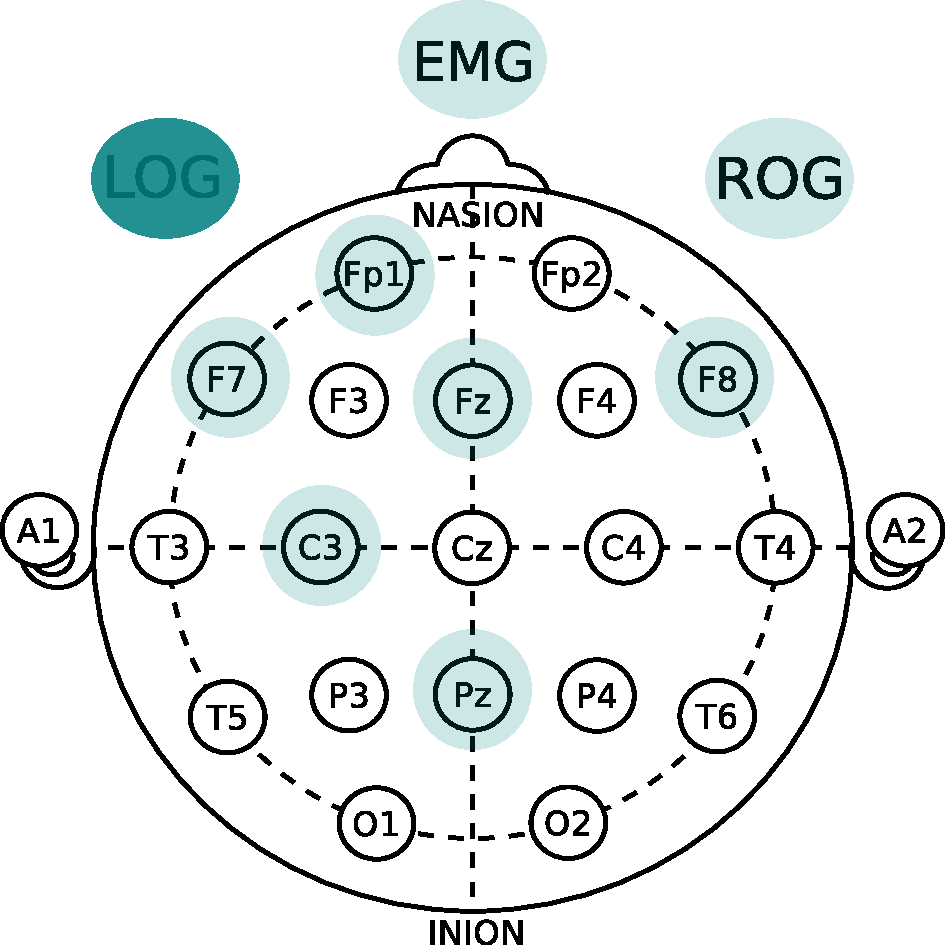
\includegraphics[width=0.17\textwidth]{./cabecitas/cabecita_RRU.pdf} &
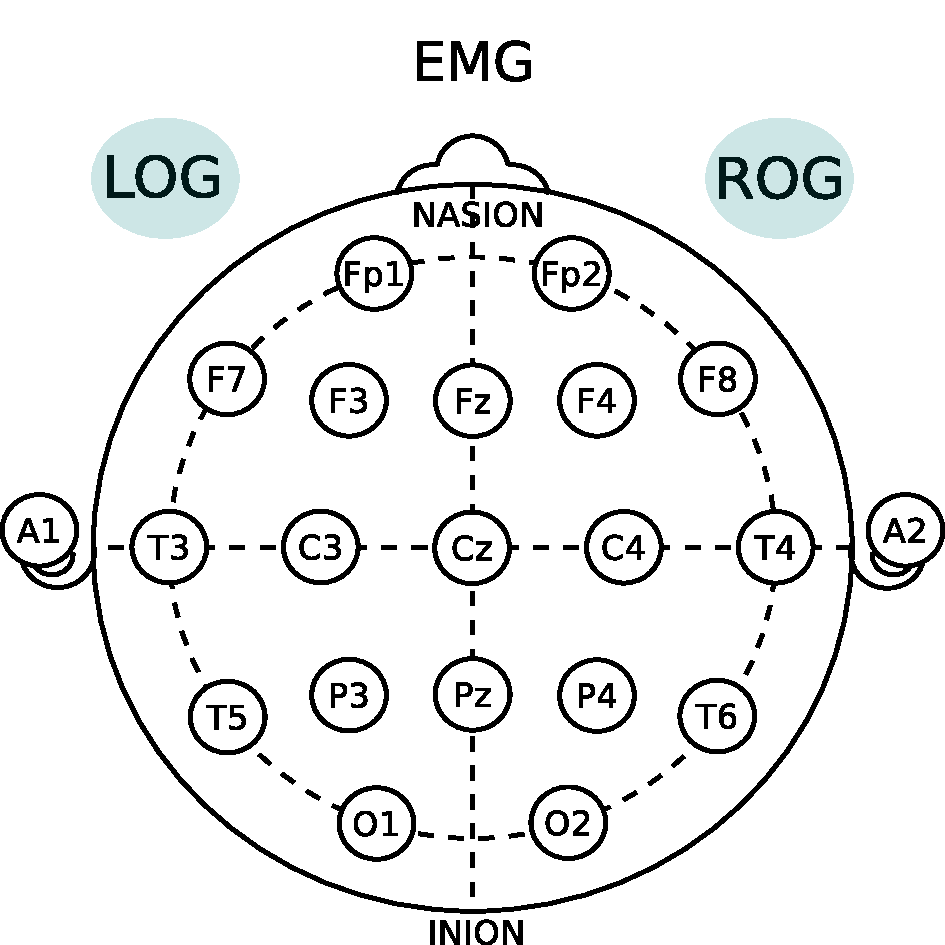
\includegraphics[width=0.17\textwidth]{./cabecitas/cabecita_JGZ.pdf} \\
CLO & RLO & RRU & JGZ
\end{tabular}
\\
\begin{tabular}{ccc}
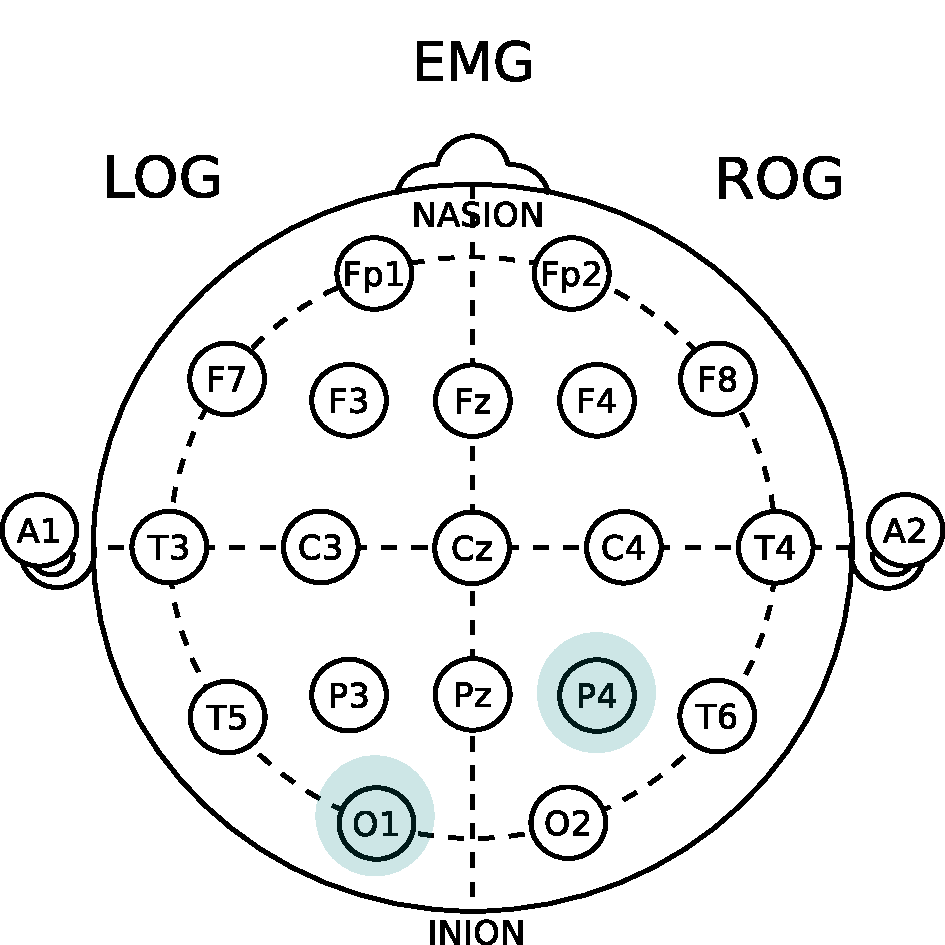
\includegraphics[width=0.17\textwidth]{./cabecitas/cabecita_FGH.pdf} &
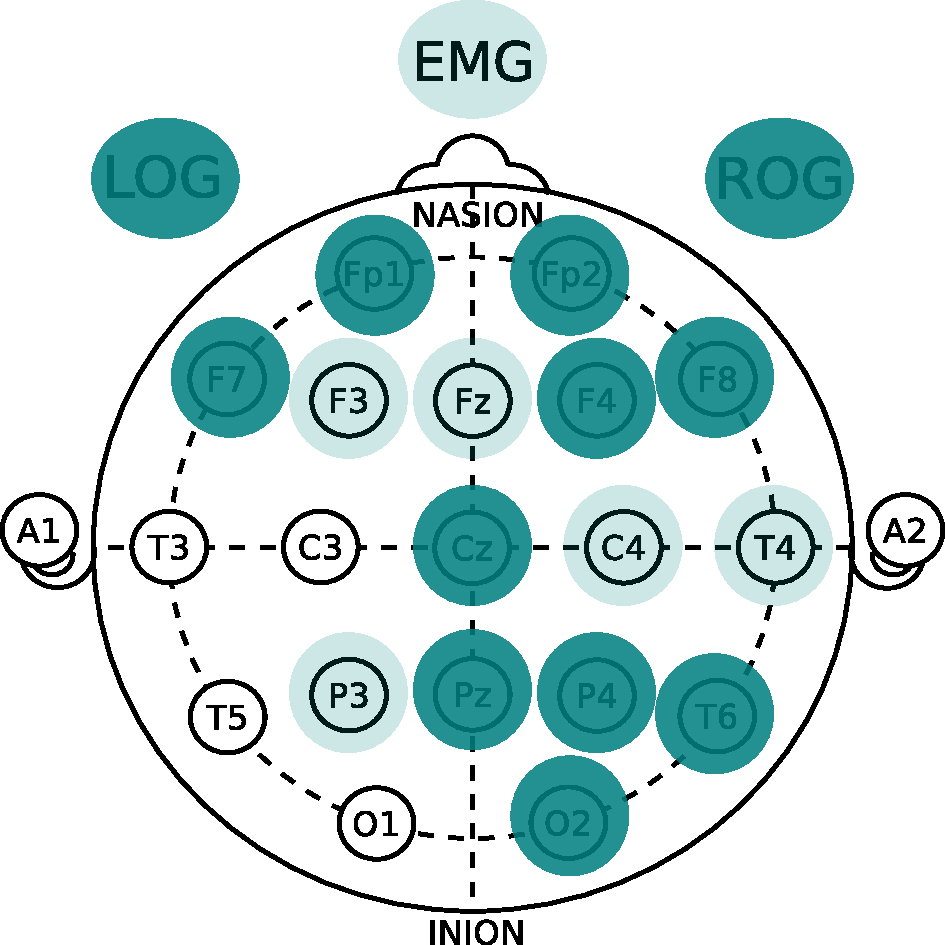
\includegraphics[width=0.17\textwidth]{./cabecitas/cabecita_MGG.pdf} &
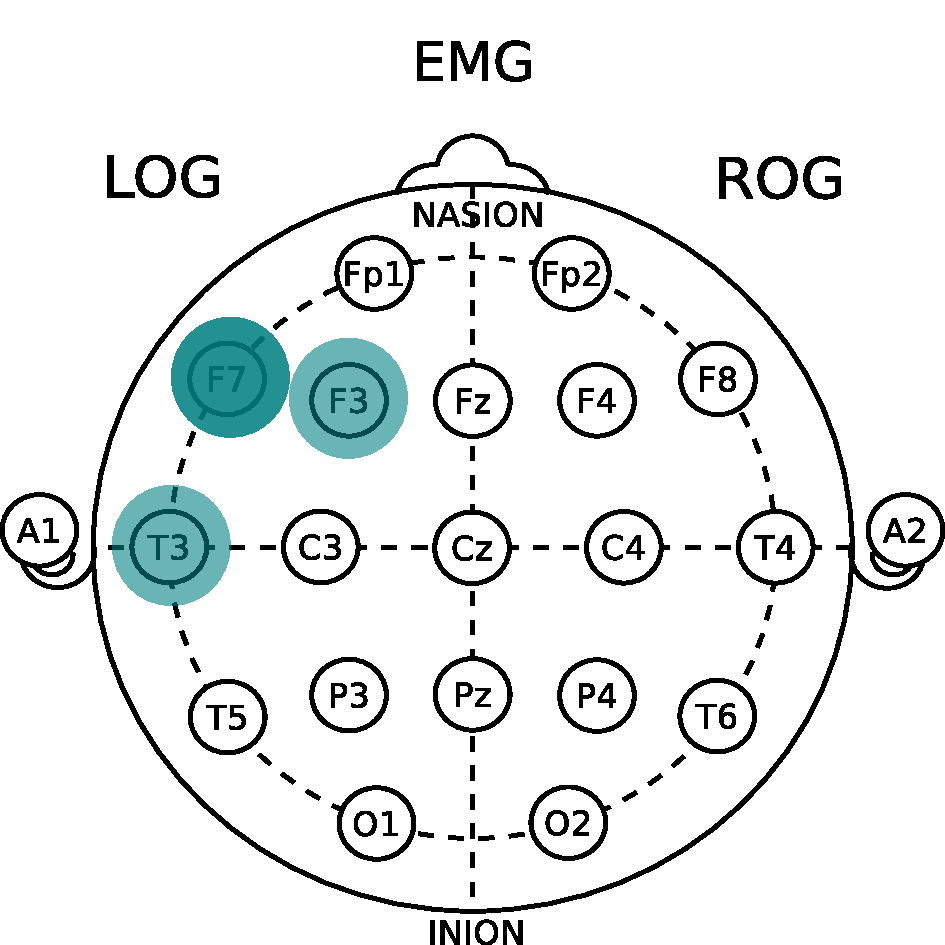
\includegraphics[width=0.17\textwidth]{./cabecitas/cabecita_EMT.pdf} \\
FGH & MGG & EMT
\end{tabular}
\end{tabular}
\caption{Representaci\'on esquem\'atica de las
diferencias significativas para la comparaci\'on entre la proporci\'on de \'epocas PE durante
sue\~no MOR y NMOR.
La intensidad del color representa el pvalor con el cual se rechaza la hip\'otesis en que las proporciones
son estad\'sticamente diferentes.}
\label{cabecitas_munchas}
\end{figure}

Posteriormente se busc\'o una diferencia m\'as directa entre los grupos, comparando grupalmente
las proporciones de \'epocas PE (en cada canal y durante las diferentes etapas). Para la 
comparaci\'on per se se us\'o la prueba U de Mann-Whitney\footnote{Implementada en R como la 
funci\'on \texttt{wilcox.test()}}.
No se encontraron diferencias significativas para ninguno de los canales, los resultados se 
muestran en las tablas \ref{gpos_mor}, \ref{gpos_nmor}, \ref{gpos_total}; para una mejor 
vizualizaci\'on, \'estos se han graficado en la figura \ref{comparacion_graf}.

\begin{figure}
\centering
\subfloat[Comparaci\'on entre \'epocas MOR (fase R)]{
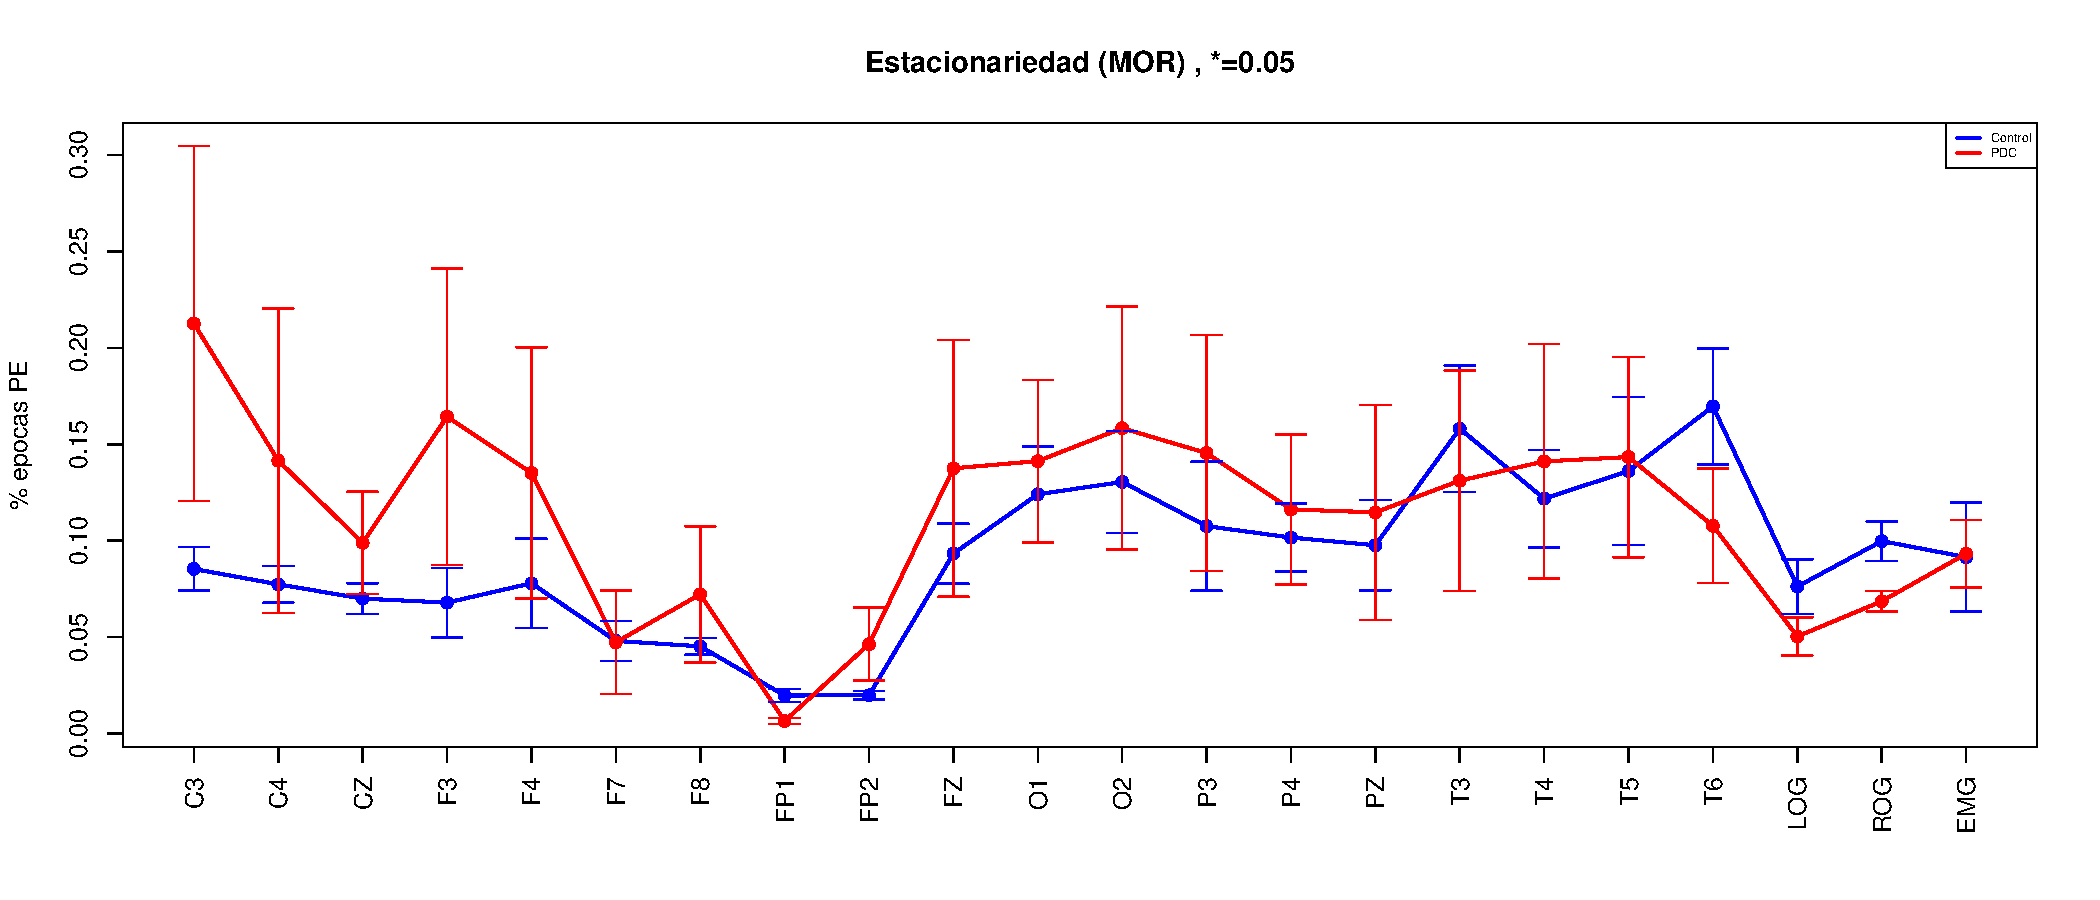
\includegraphics[width=0.95\linewidth]
{./new170424/Comparacion_gpos_MOR.pdf} 
}\\
\subfloat[Comparaci\'on entre \'epocas no-MOR (fases W y N)]{
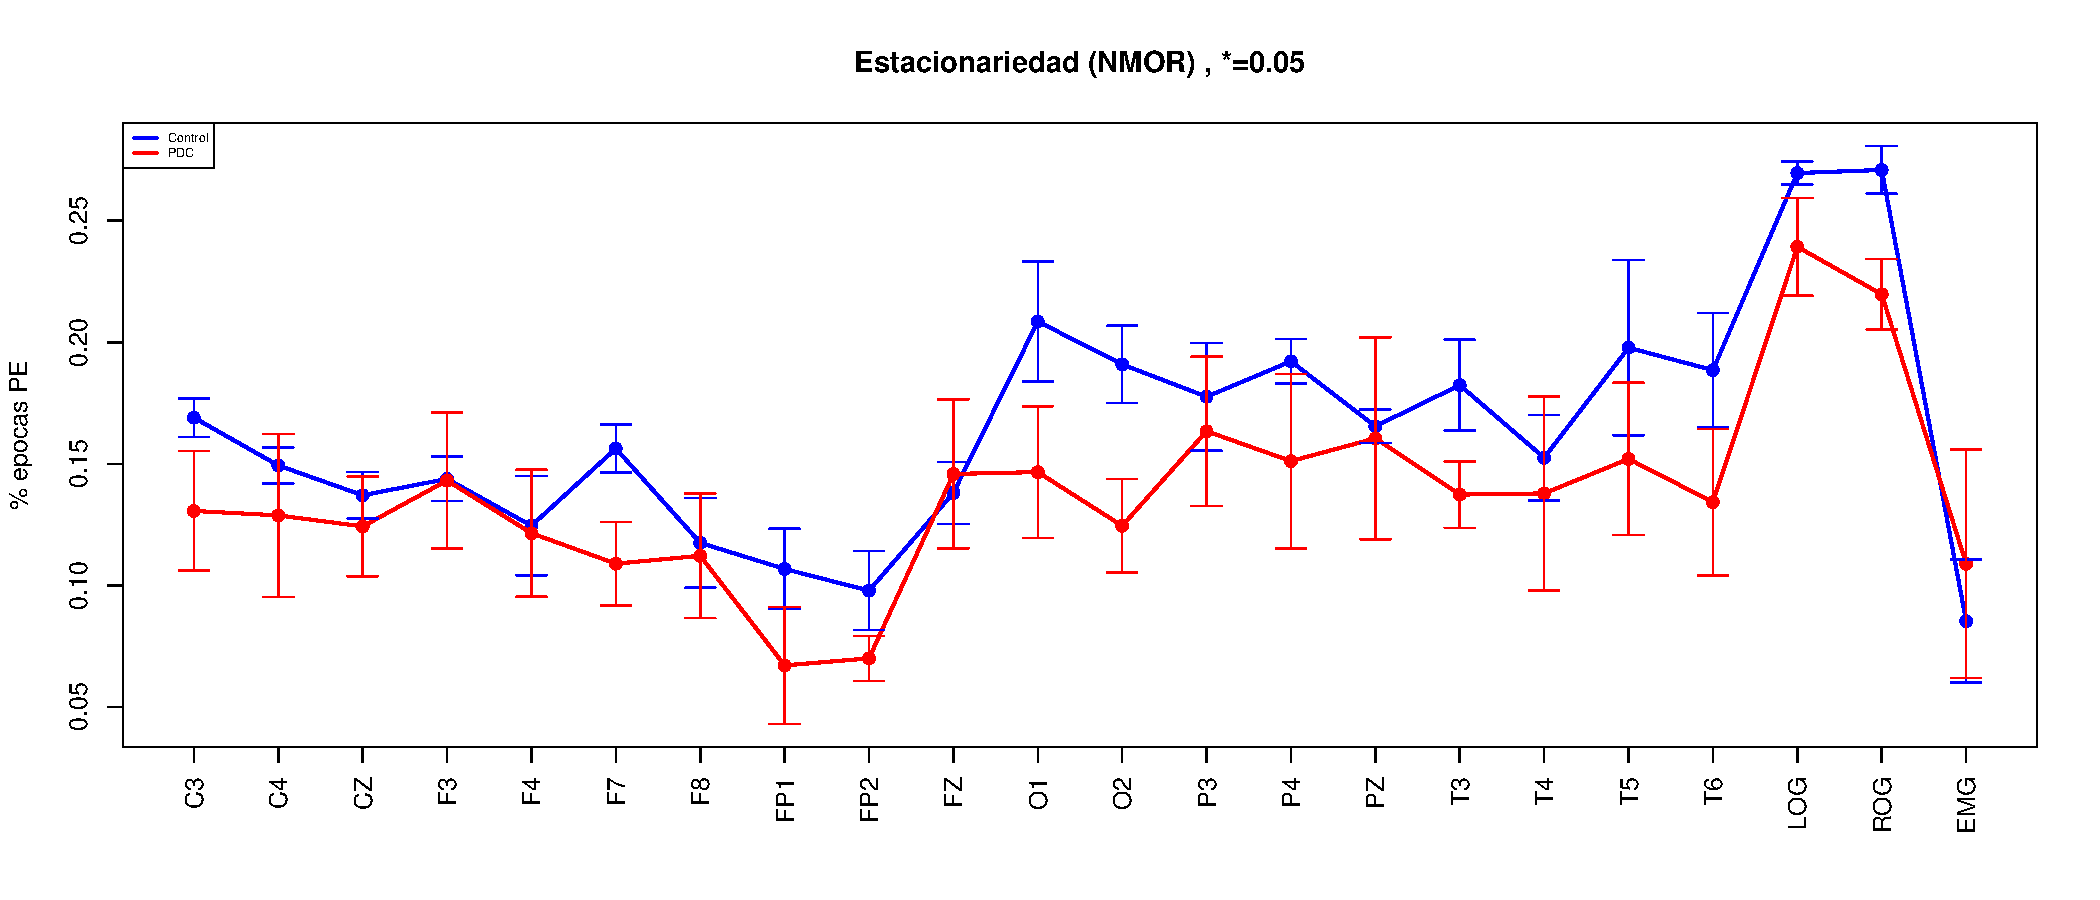
\includegraphics[width=0.95\linewidth]
{./new170424/Comparacion_gpos_NMOR.pdf} 
}\\
\caption{Comparaci\'on sobre las proporciones de \'epocas PE entre los grupos Control (azul) y
PDC (rojo), para diferentes etapas de sue\~no (MOR y NMOR). Se grafica el promedio grupal $\pm$
1 desviac\'on est\'andar $^{\nicefrac{3}{2}}$, como visualizaci\'on aproximada de la varianza.}
\label{comparacion_graf}
\end{figure}

Una segunda variaci\'on del primer an\'alisis es considerar grupalmente a los sujetos como 
'unidades' que transitan entre etapas de sue\~no; se comparan grupalmente las proporciones de 
\'epocas PE --en cada canal-- durante sue\~no MOR y NMOR, usando la prueba U de Mann-Whithney;
en la figura \ref{comparacion_verde} se han representado gr\'aficamente estas diferecias.
Se encontr\'o que hay diferencias significativas ($\alpha<0.1$) para el grupo Control en los 
canales C3, C4, F7, F8, FP1, FP2, O2, P4, LOG y ROG, mientras que en el grupo PDC s\'olo se
observaron diferencias en LOG y ROG.
Descartando los canales LOG y ROG, ya que no son parte del EEG, las diferencias encontradas 
pueden ser relevantes fisiol\'ogicamente, ya que abarcan gran parte de los l\'obulos frontal y 
parietal, y parte de la regi\'on occipital-parietal derecha; en la figura \ref{cabecita} se
indican esquem\'aticamente estas regiones.

\begin{figure}
\centering
\subfloat[Comparaci\'on para el grupo control]{
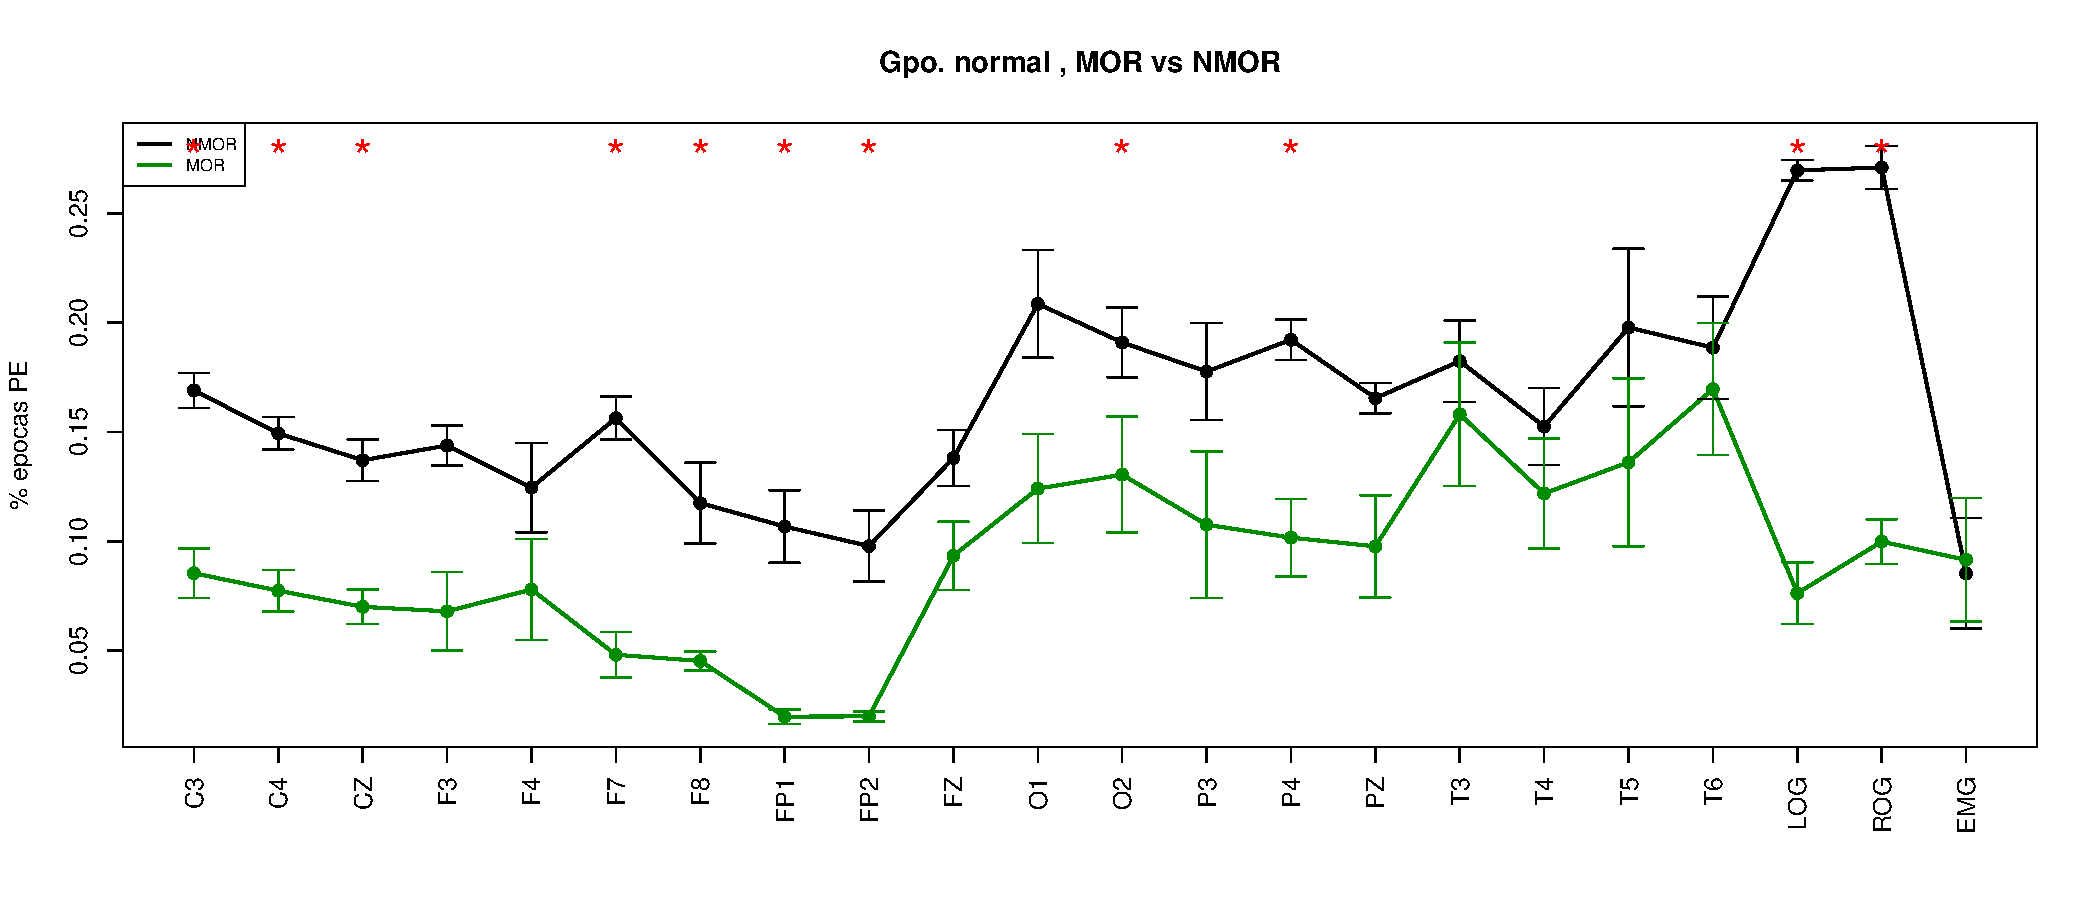
\includegraphics[width=0.95\linewidth]
{./new170424/comp_etapas_gpos_NORMALMOR_vs_NMOR.pdf} 
}\\
\subfloat[Comparaci\'on para el grupo PDC]{
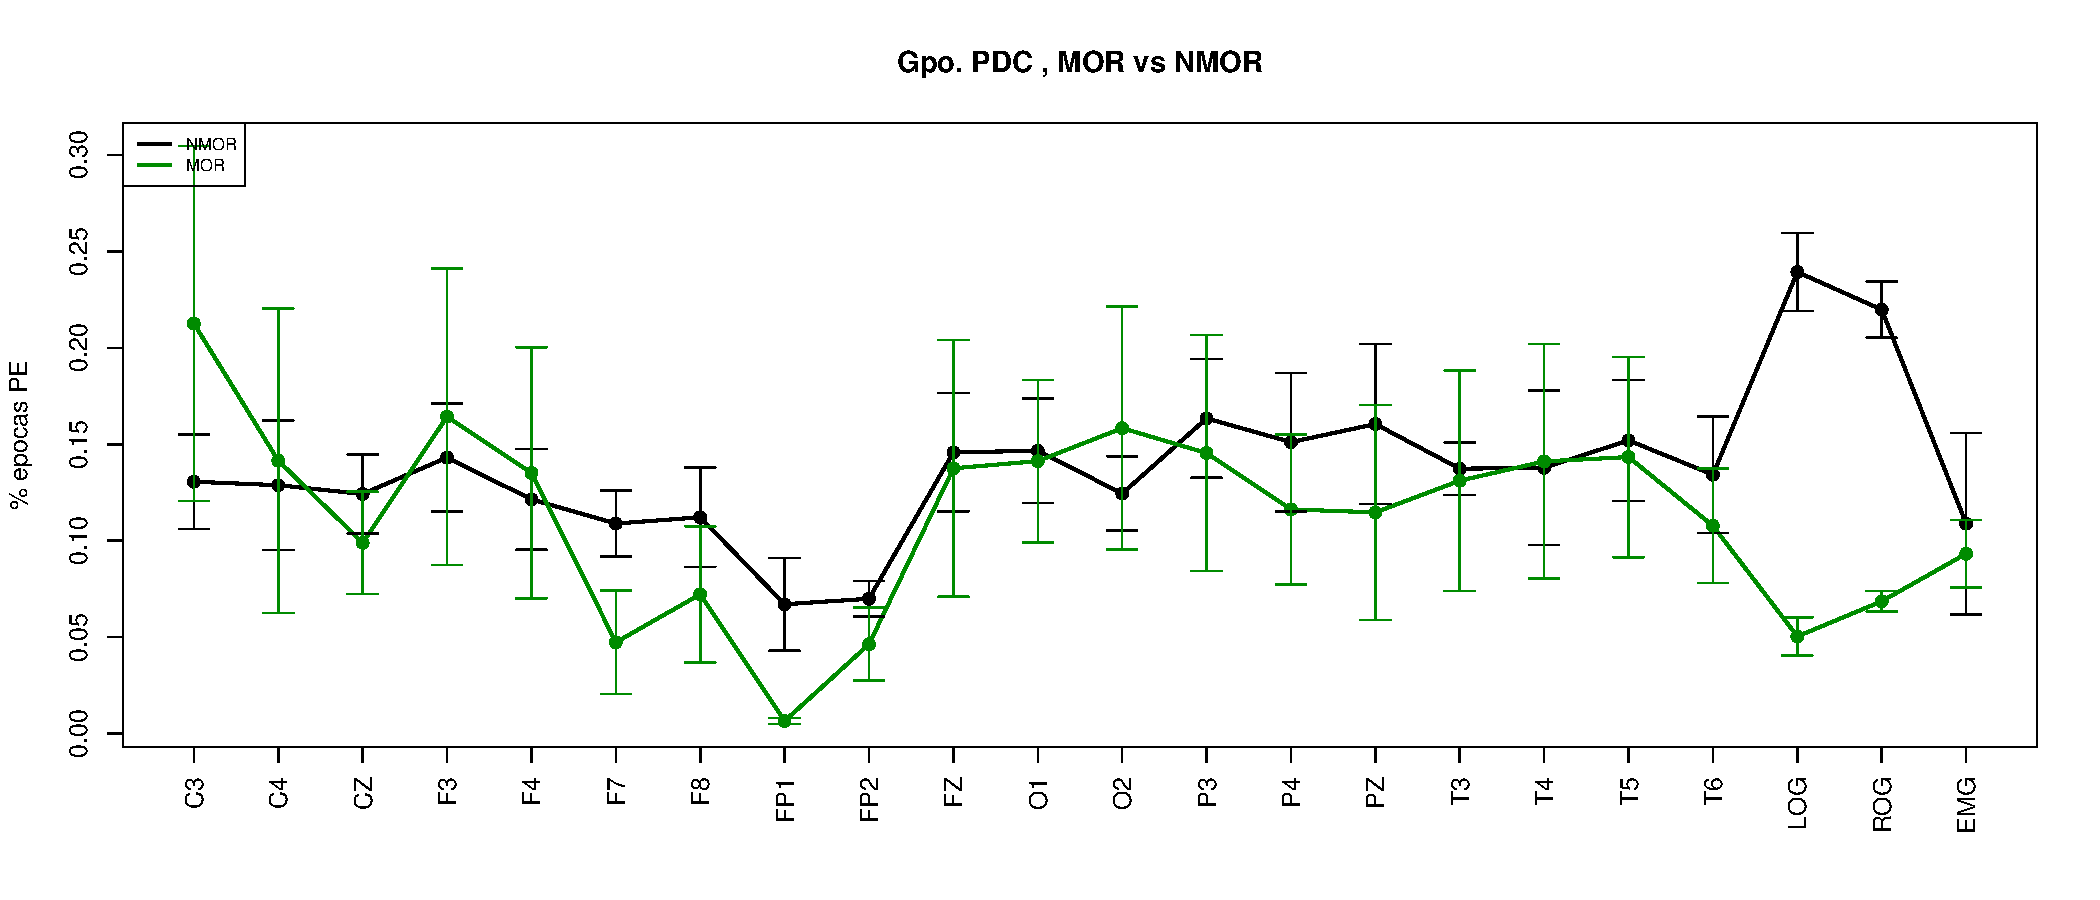
\includegraphics[width=0.95\linewidth]
{./new170424/comp_etapas_gpos_PDCMOR_vs_NMOR.pdf} 
}
%\\
%\subfloat[Comparaci\'on de los p-valores para aceptar diferencias]{
%\includegraphics[width=0.95\linewidth]
%{./new170424/Comparacion_pvals_gpos_MOR_vs_NMOR.pdf} 
%}\\
\caption{Comparaci\'on sobre las proporciones de \'epocas PE entre las etapas de sue\~no MOR
(verde) y NMOR (negro), para ambos grupos por separado. 
Se han graficado las proporciones de PE en todos los sujetos de cada grupo, para todo el sue\~no y 
la etapa MOR.
Se grafica el promedio grupal $\pm$
1 desviac\'on est\'andar $^{\nicefrac{3}{2}}$, como visualizaci\'on aproximada de la varianza.}
\label{comparacion_verde}
\end{figure}

\begin{figure}
\centering
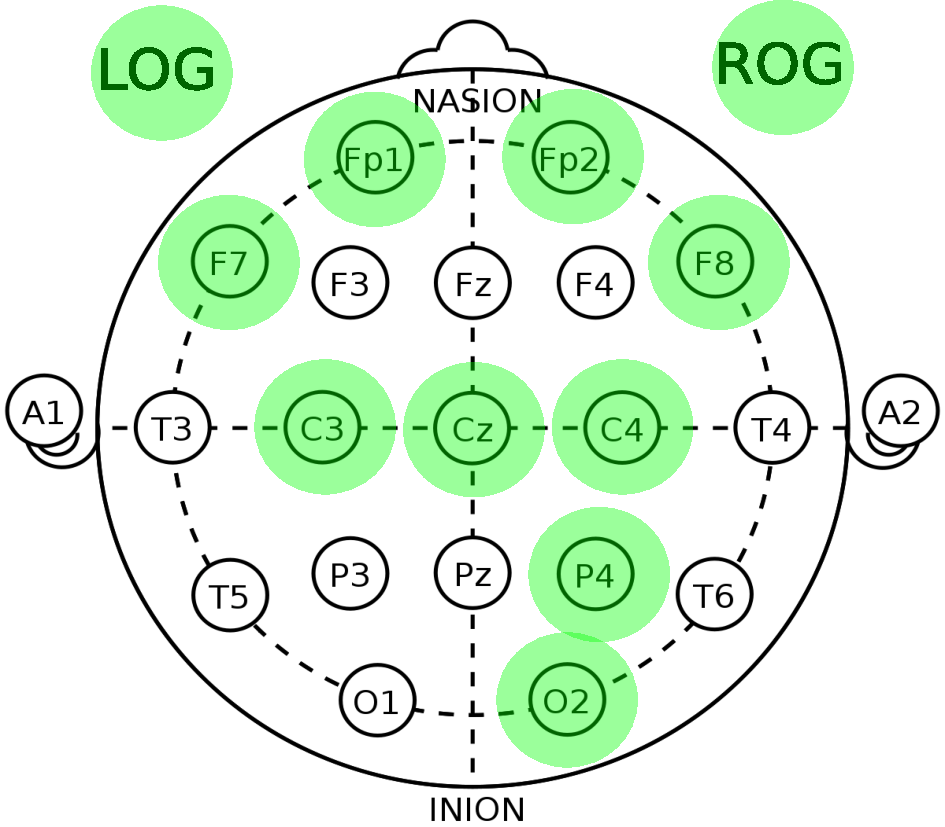
\includegraphics[width=0.4\linewidth]
{cabecita.pdf} 
\caption{Representaci\'on esquem\'atica de los sitios donde se encontraron diferencias 
significaticas en la comparaci\'on entre el porcentaje de \'epocas PE durante sue\~no MOR y NMOR,
para el grupo Control (ver texto)}
\label{cabecita}
\end{figure}

\section{Patrones visuales}

%Se encontrar\'o una serie de patrones visuales que surgen cuando los datos obtenidos son 
%graficados tomando en cuenta el tiempo, y que parecen contener informaci\'on relevante respecto a 
%la aparici\'on del sue\~no MOR.
Como un an\'alisis exploratorio, buscando explicar la variabilidad entre los resultados, se 
graficaron los resultados obtenidos con el test PSR de la siguiente manera: se colocan en 
l\'inea horizontal una serie de cuadros, uno por cada \'epoca analizada seg\'un fue clasificada 
(blanco: PE, negro: no-estacionario), y posteriormente se juntaron verticalmente las l\'ineas
correspondientes a los diferentes canales; en la figura \ref{ejemplo_graf} se muestra un ejemplo de
ello, mientras que en el anexo se muestran los gr\'aficos construidos para cada uno de los sujetos. 

Al construir estos gr\'aficos, se hacen presentes 'bloques' de \'epocas que en su mayor\'ia son
PE --similarmente con \'epocas no-estacionarias. Ha parecido conveniente reportar este hallazgo
ya que los patrones son consistentes en todos los sujetos, y porque parece que estos 'bloques'
aparecen asociados al sue\~no MOR en cierto orden (ilustrado en la figura \ref{patroncito}):
\begin{itemize}
\item Bloque abundante en \'epocas PE, visualmente oscuro
\item Bloque abundante en \'epocas no-estacionarias, visualmente claro
\item Secci\'on que contiene el sue\~no MOR, los canales LOG y ROG muestran son visualmente m\'as
abundante en \'epocas no-estacionarias en esta zona del tiempo
\end{itemize}

%@{.}

\begin{figure}
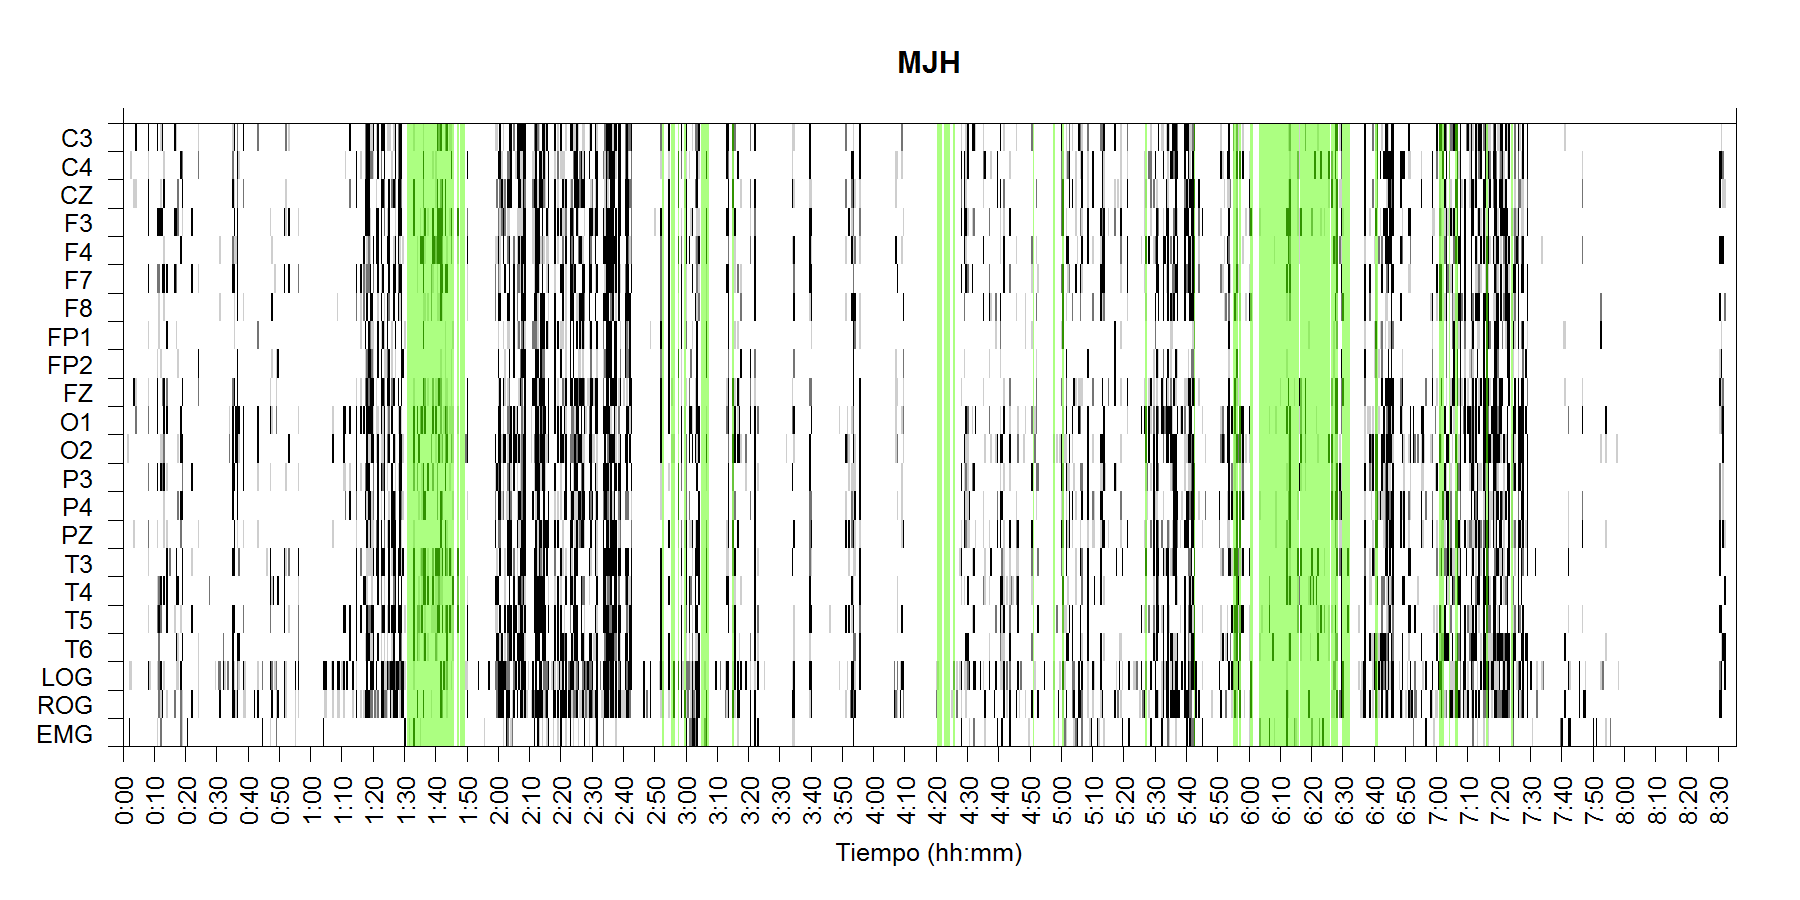
\includegraphics[width=\textwidth]
{./g170413/MJNNVIGILOS_est.png}
\caption{Disposici\'on gr\'afica para los resultados del test PSR en el sujeto MJH. 
%En el eje 
%horizontal se muestra el tiempo desde el inicio de registro, mientras que en el eje vertical se 
%encuentra el nombre del canal. 
Se han resaltado con color verde las \'epocas clasificadas como de sue\~no MOR.
}
\label{ejemplo_graf}
\end{figure}

\begin{figure}
\includegraphics[width=\textwidth]
%{./complementario170409/patrones_MJH.png}
{./graphs170427/zoom_MJH.pdf}
\caption{Se ha resaltado el patr\'on visual que, se propone, est\'a asociado con la aparici\'on del
sue\~no MOR: un bloque de \'epocas PE (rojo), un bloque de \'epocas no-estacionarias (azul) y un 
bloque que contiene al sue\~no MOR.}
\label{patroncito}
\end{figure}

%%%%%%%%%%%%%%%%%%%%%%%%%%%%%%%%%%%%%%%%%%%%%%%%%%%%%%%%%%%%%%%%%%%%%%%%%%%%%%%%%%%%%%%%%%%%%%%%%%%
%%%%%%%%%%%%%%%%%%%%%%%%%%%%%%%%%%%%%%%%%%%%%%%%%%%%%%%%%%%%%%%%%%%%%%%%%%%%%%%%%%%%%%%%%%%%%%%%%%%
%%%%%%%%%%%%%%%%%%%%%%%%%%%%%%%%%%%%%%%%%%%%%%%%%%%%%%%%%%%%%%%%%%%%%%%%%%%%%%%%%%%%%%%%%%%%%%%%%%%
%%%%%%%%%%%%%%%%%%%%%%%%%%%%%%%%%%%%%%%%%%%%%%%%%%%%%%%%%%%%%%%%%%%%%%%%%%%%%%%%%%%%%%%%%%%%%%%%%%%

\section{Discusi\'on}

Como se mencion\'o en la secci\'on de hip\'otesis, este trabajo pare del supuesto en que los
sujetos con PDC presentan con mayor probabilidad estacionariedad d\'ebil en sus registros de EEG.
Se ha aportado evidencia para afirmar que no hay cambios significativos en la porci\'on de tiempo 
durante la cual el registro de PSG se comporta de manera 'simple', al comparar sujetos cntrol y con
PDC. Esto puede interpretarse como que --quiz\'a-- los mecanismos afectados durante el PDC no 
provocan que la se\~nal se vuelva m\'as 'simple' en el sentido de volverse estacionaria.

Cabe un comentario sobre c\'omo la evidencia presentada exhibe al PSG como un conjunto de se\~nales 
mayoritariamente no-estacionarias, y que se comportan como estacionarias por una porci\'on m\'as
bien peque\~na del sue~no nocturno; luego entonces, no es adecuado analizar este tipo de se\~nales 
con m\'etodos que supongan estacionariedad --por ejemplo, an\'alisis cl\'asico de Fourier. 
M\'as a\'un este comentario se acent\'ua en individuos con PDC.

\subsection{La inclusi\'on de sujetos}

Durante el trabajo se menciona constantemente a tres sujetos (FGH, MGG, EMT) cuyos registros de PSG 
fueron analizados pero que no son considerados estad\'isticamente; cada uno de ellos fue exclu\'ido 
del trabajo original \cite{VazquezTagle16} por diversos motivos, pero dieron su consentimiento 
informado para el registro de PSG, debido a lo cual se decidi\'o analizar el efecto de su 
inclusi\'on dentro de los estad\'isticas.

El caso m\'as notorio es el sujeto FGH, quien padece de par\'alisis facial, cataratas, y problemas 
no especificados en la hipotiroides y la columna. Seg\'un se reporta, el sujeto no inform\'o de 
estos padecimientos sino hasta despu\'es del registro de PSG, por lo que su exlusi\'on se efectu\'o 
a posteriori.

Dentro del marco de este trabajo, son destacableslas proporciones inusuales de \'epocas PE para 
este sujeto en los canales F4, F7, F8, FP1, FP2, FZ, tanto en sue\~no MOR como no-MOR; estas 
haciendo uso de la representaci\'on gr\'afica mencionada, la estructura de estos datos es m\'as
inusual a\'un (figura \ref{FGH_especial}).
Como comentario, un vistazo a estos resultados inusuales pudiera haber delatado las 
caracter\'isticas de este sujeto, si bien esta metodolog\'ia no se usa expl\'icitamente para tal 
fin.

\begin{figure}
\centering
\includegraphics[width=0.95\linewidth]
{./muypreeliminar170408/FGHSUE_est.png} 
\caption{Compilado gr\'afico para el sujeto FGH; n\'otese la }
\label{FGH_especial}
\end{figure}

%%%%%%%%%%%%%%%%%%%%%%%%%%%%%%%%%%%%%%%%%%%%%%%%%%%%%%%%%%%%%%%%%%%%%%%%%%%%%%%%%%%%%%%%%%%%%%%%%%%
%%%%%%%%%%%%%%%%%%%%%%%%%%%%%%%%%%%%%%%%%%%%%%%%%%%%%%%%%%%%%%%%%%%%%%%%%%%%%%%%%%%%%%%%%%%%%%%%%%%

\subsection{Efecto del tama\~no de las \'epoca}

El uso de \'epocas de 30 segundos est\'a motivado por las recomendaciones de la AAMS para 
clasificar, de manera estandarizada, las etapas de sue\~no a partir de registros de PSG 
\cite{AASM07}. 
No se discutir\'an en este trabajo motivaciones o evidencia para usar esta longitud de \'epoca en 
particular, ni para el caso contrario, sino que se acepta por fines de comparabilidad. 
Sin embargo, debido a un problema t\'ecnico, en alg\'un momento de este trabajo se usaron los 
registros de PSG organizados en \'epocas de 10 segundos de duraci\'on; se realizaron los an\'alisis 
descritos usando esta segmentaci\'on mixta (algunos sujetos con \'epocas de 10 s, otros con 
\'epocas de 30 s) y se obtuvieron resultados seg\'un los cuales no hay diferencias significativas 
en ninguno de los an\'alisis. 
Por otro lado, la representaci\'on gr\'afica construida a partir de los mismos datos, organizados
en \'epocas de 10 s, cambia sustancialmente (ver figura \ref{comp_VCR}).

%El hecho de que los resultados fueran afectados de manera contundente por la forma en que se 
%organizan los datos, sugiere que ser\'a provechoso prestar mayor atenci\'on a la naturaleza de las 
%caracter\'isticas estudiadas y su posible interpretaci\'on en la fisiolog\'ia.

%\begin{figure}
%\centering
%\subfloat[Comparaci\'on entre \'epocas MOR (fase R)]{
%\includegraphics[width=0.95\linewidth]
%{./material170331/Comparacion_gpos_MOR.pdf} 
%}\\
%\subfloat[Comparaci\'on entre \'epocas no-MOR (fases W y N)]{
%\includegraphics[width=0.95\linewidth]
%{./material170331/Comparacion_gpos_NMOR.pdf} 
%}\\
%\caption{Comparaci\'on sobre las proporciones de \'epocas PE entre los grupos, para diferentes
%etapas de sue\~no; se han usado los datos calculados con la segmentaci\'on de los
%registros en \'epocas de 30s y 10 s replicando un detalle t\'ecnico.}
%\label{comparacion_graf_mixto}
%\end{figure}

\begin{figure}
\centering
\subfloat[Usando \'epocas de 10 s]{
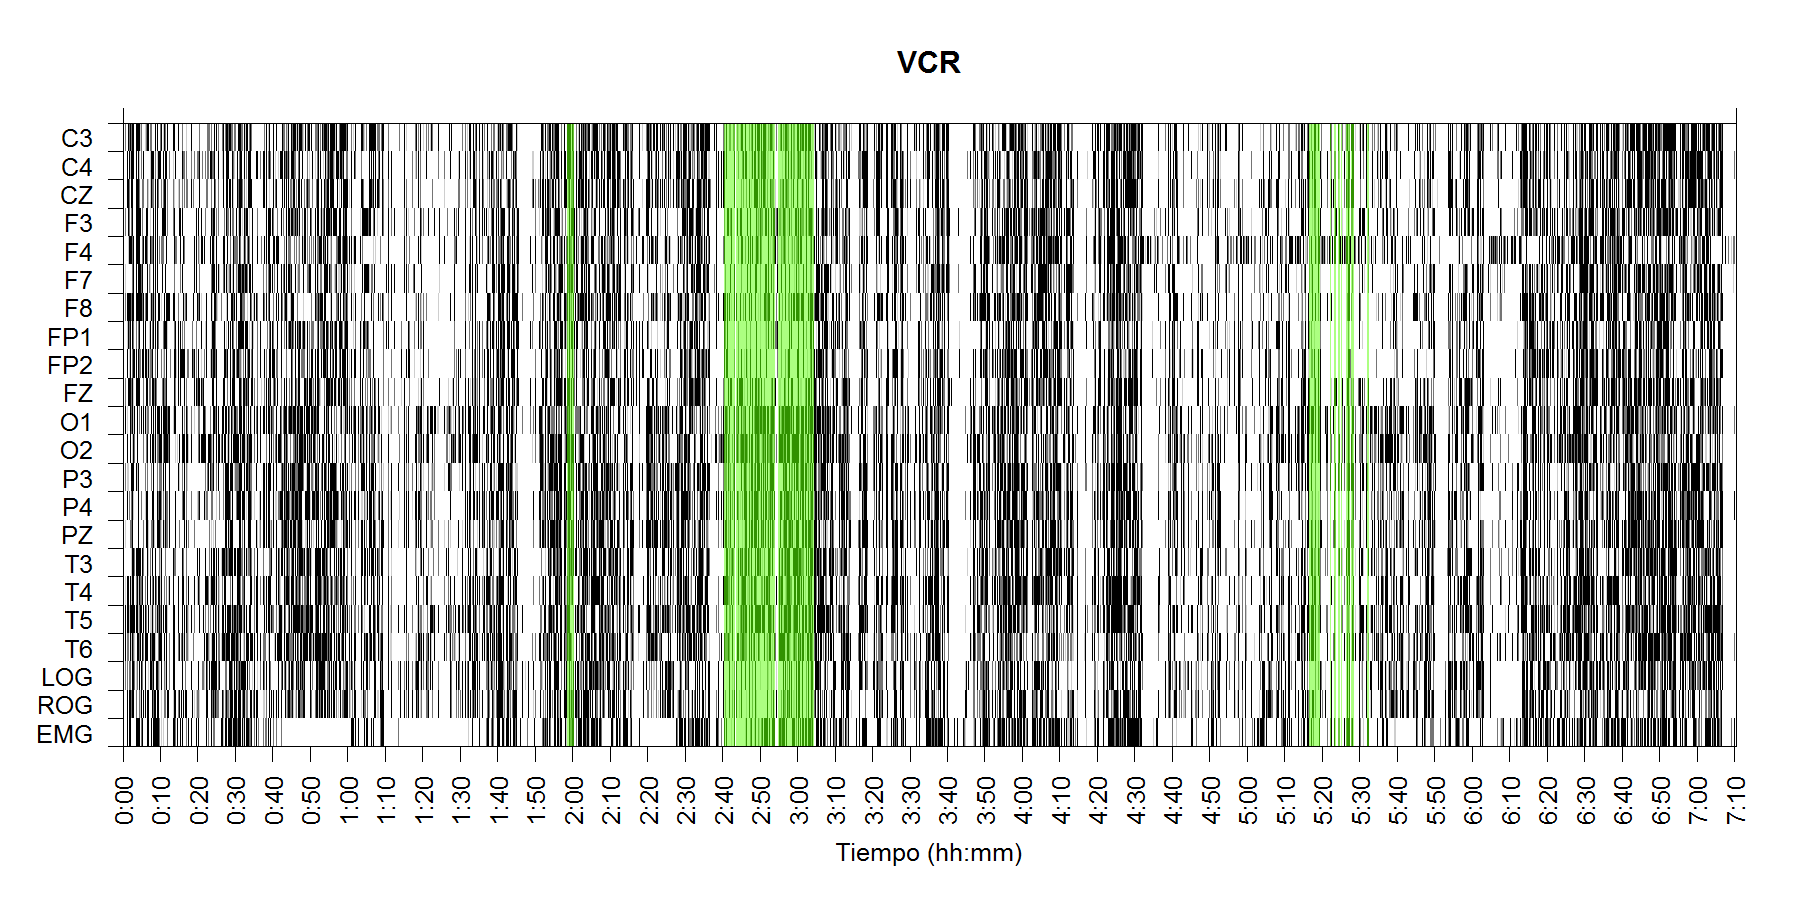
\includegraphics[width=0.95\linewidth]
{./grafiquitos170404/VCNNS1_est.png} 
}\\
\subfloat[Usando \'epocas de 30 s]{
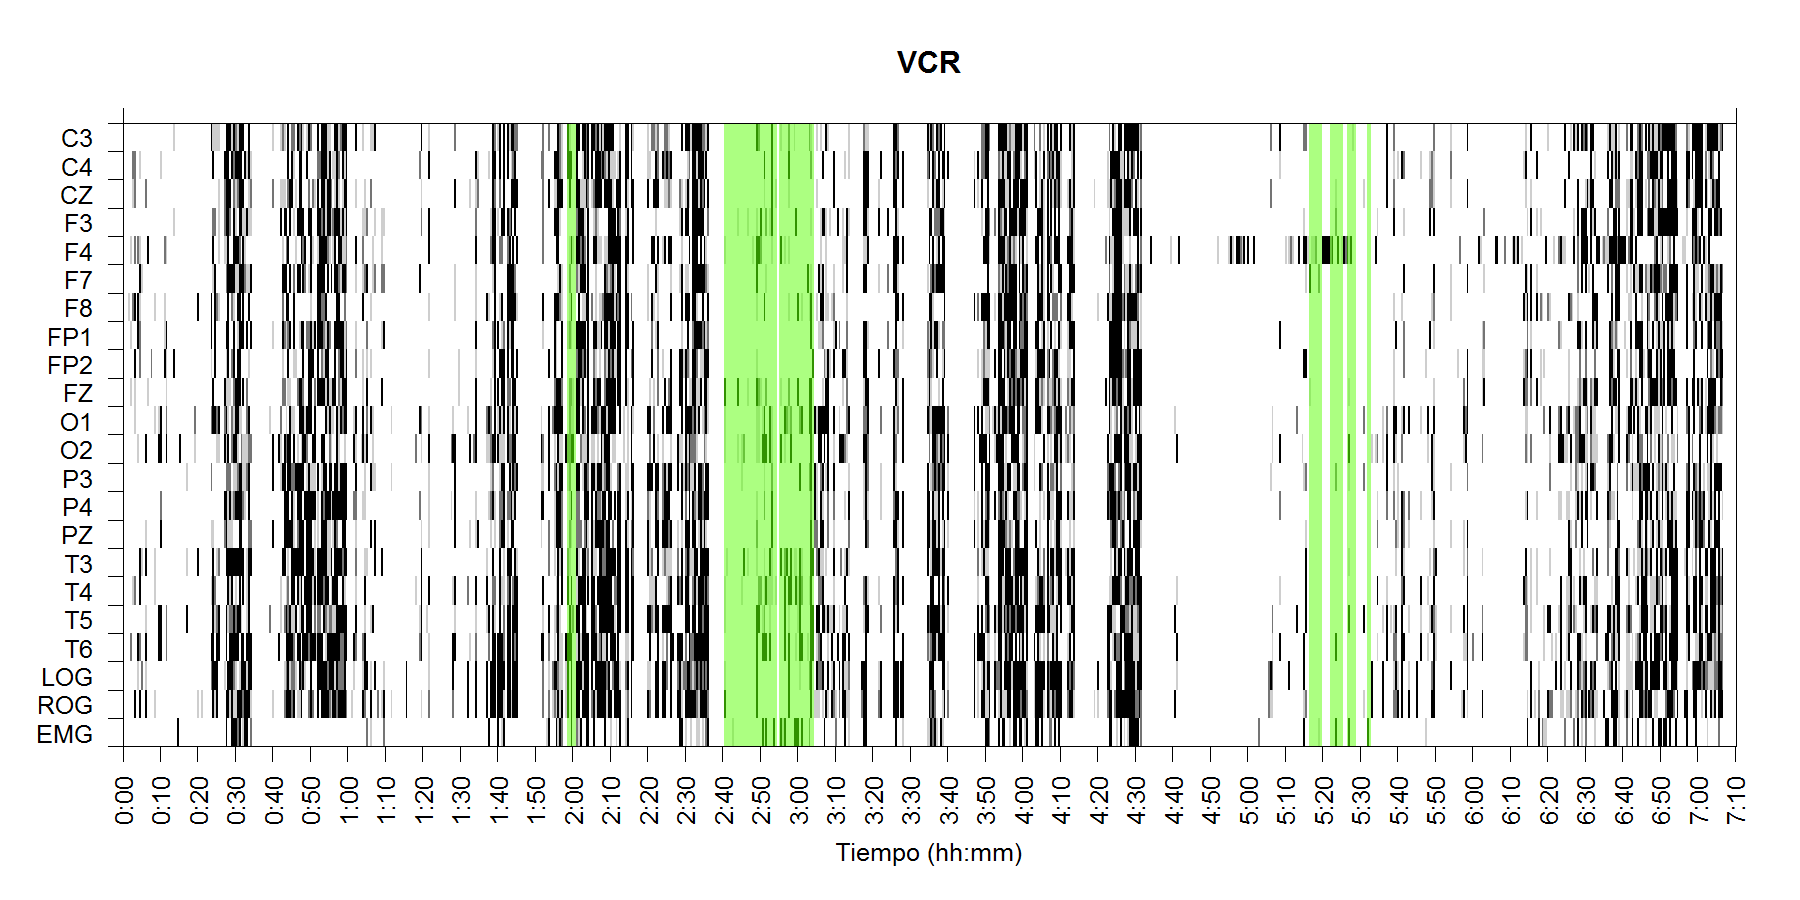
\includegraphics[width=0.95\linewidth]
{./muypreeliminar170408/VCNNS1_est.png} 
}\\
\caption{Compilaci\'on gr\'afica de las \'epocas clasificadas como PE, distribuidas en el tiempo
para cada uno de los canales. El registro corresponde al sujeto VCR dado que su registro fuera
segmentado de dos maneras difrentes, variando la duraci\'on de las \'epocas.}
\label{comp_VCR}
\end{figure}

El hecho de que los resultados fueran afectados de manera contundente por la forma en que se 
organizan los datos, sugiere que ser\'a provechoso prestar mayor atenci\'on a la naturaleza de las 
caracter\'isticas estudiadas y su posible interpretaci\'on en la fisiolog\'ia.
Se propone que los registros de PSG tienen una propiedad referida como 'estacionariedad local'
(definici\'on \ref{est_local}), concepto introducido por Dahlhaus \cite{Dahlhaus97}.
A grosso modo, un proceso localmente estacionario es aqu\'el cuya SDF --que puede depender del 
tiempo-- puede ser aproximada 'a trozos': usando SDF's correspondientes a procesos que poseen una 
representaci\'on espectral de Cram\'er, que est\'an definidos para el intervalo de tiempo $[0,1]$ 
y que est\'an 'correctamente ensamblados'.

\begin{defn}[Estacionariedad local]
Una secuencia de procesos estoc\'asticos de media cero, 
$\{ X_{t,N} \}$ con $t = 1, 2, \dots, N$, se dicen localmente estacionarios en el 
tiempo $t_0 \in [0,1]$ si existe una representaci\'on del tipo
\begin{equation*}
X_{t,N} = \intPI \widetilde{A_{t,N}}(\omega) e^{i \omega t} dZ(\omega)
\end{equation*}
donde se satisface que:
\begin{itemize}
\item $\{ Z(\omega) \}$ es un proceso de media cero con incrementos ortogonales, es decir
\begin{equation*}
\Cov{dZ(\omega_1),dZ(\omega_2)} =
\begin{cases}
d\omega &\text{, } \omega_1 = \omega_1 \\
0 &\text{, otro caso}
\end{cases}
\end{equation*}
\item Existe una constante $K$ y una funci\'on suave 
$A: [0,1]\times [-\pi,\pi] \rightarrow \mathbb{C}$, 
con $A(t_0,\omega) = \overline{A(t_0,-\omega)}$, tal que para toda $N$
\begin{equation*}
\sup_{\nicefrac{t}{N}\in \varepsilon_N(t_0)} 
\sup_{\omega} \abso{ \widetilde{A_{t,N}}(\omega) - A(t_0,\omega) }
\leq \frac{K}{N}
\end{equation*}
con $\varepsilon_N(t_0)$ es una vecindad de $t_0$ 
tal que $\abso{\abso{\nicefrac{t}{N}-t_0}} = O(N^{-\alpha})$,
%cuyo tama\~no es del orden $O(N^{-\alpha})$,
con $0\leq \alpha < 1$
\item $A(t_0,\omega)$ es continuo en $\{ t_0 \} \times [-\pi,\pi]$
\end{itemize}
\label{est_local}
\end{defn}

Se propone que los registros de PSG se comportan como procesos localmente estacionarios; m\'as 
a\'un, esta caracter\'istica podr\'ia cambiar en adultos mayores con y sin PDC. 
Una motivaci\'on fisiol\'ogica para la hip\'otesis anterior es el contenido de los registros de
PSG: un conjunto descoordinado y homog\'eneo de ondas cerebrales, complejos K y husos de sue\~no.
Si bien esta composici\'on sugiere que la no-estacionariedad es la opci\'on m\'as obvia, el
an\'alisis llevado a cabo revela que el contenido de estos eventos no es homog\'eneo durante el
sue\~no; m\'as a\'un, mientras m\'as peque\~no sea el intervalo de tiemo observado, es m\'as
posible encontrar zonas de composici\'on m\'as o menos homog\'enea que puedan ser clasificadas
como PE.
Esta hip\'otesis explicar\'ia el cambio observado al cambiar el tama\~no de la \'epoca; de manera
arriesgada, se podr\'ia concluir que, entre los individuos con PDC, la homogeneidad del PSG es muy
similar durante MOR y NMOR.
Sin embargo, para poder convertir esta hip\'otesis en una conclusi\'on aut\'entica, faltar\'ia
m\'as investigaci\'on al respecto --en particular, una prueba para detectar estacionariedad local.

%La hip\'otesis de la estacionariedad local trae a la discusi\'on un detalle muy particular: tal 
%cual est\'a escrita, esta definici\'on carece de utilidad pr\'actica para ser detectada en una 
%serie de tiempo dada. El enfoque m\'as intuitivo es que como un proceso localmente estacionario 
%puede ser aproximado como 'uni\'on' de procesos d\'ebilmente estacionarios (equivalentemente, 
%como una sucesi\'on de procesos 'd\'ebilmente estacionarios a trozos'), tiene sentido intentar 
%construir esos procesos; sin embargo, el verdadero problema es garantizar la convergencia de 
%estas aproximaciones. En este trabajo no se ha investigado suficiente al respecto, pero parece 
%una alternativa plausible para explicar los fen\'omenos hallados.

%Con respecto a la hip\'otesis de los eventos, bien puede tomarse un enfoque de reconocimiento de
%patrones, ''contando'' las incidencias de eventos y revisando si se relaciona con la
%clasificaci\'on como PE. Ese enfoque va m\'as all\'a de los objetivos de este trabajo.

%%%%%%%%%%%%%%%%%%%%%%%%%%%%%%%%%%%%%%%%%%%%%%%%%%%%%%%%%%%%%%%%%%%%%%%%%%%%%%%%%%%%%%%%%%%%%%%%%%%
%%%%%%%%%%%%%%%%%%%%%%%%%%%%%%%%%%%%%%%%%%%%%%%%%%%%%%%%%%%%%%%%%%%%%%%%%%%%%%%%%%%%%%%%%%%%%%%%%%%

\section{Conclusiones}

En registros 
de PSG para adultos mayores, segmentado en \'epocas de 30 segundos,
la presencia proporcional de estacionariedad d\'ebil  
es signitivamente diferente durante el sue\~no MOR y NMOR.
Estas diferencia se pudieron observar en el grupo Control
%en sujetos control 
para los canales 
C3, C4, F7, F8, FP1, FP2, O2, P4, LOG, ROG; en el grupo con PDC 
s\'olo se detectaron estas 
diferencias para los canales LOG y ROG.
Estos cambios entre MOR y NMOR pueden explicarse (1) en LOG y ROG 
por las caracter\'isticas propias del sue\~no MOR, y (2) en el resto de los canales
--para el grupo control-- porque se tratan de la regi\'on frontal, asociada a la
toma de decisiones, y posterior, asociada con la memoria.

%sujetos con y sin PDC diagnosticado.
%Luego entonces, esta caracter\'istica no es un indicador fiable 
Las diferencias grupales no se expresan claramente al considerar individualmente
a los sujetos excepto en los canales LOG y ROG, siendo consistente este dato con la 
caracterizaci\'on del sue\~no MOR: movimientos oculares r\'apidos y aton\'ia muscular.
Se concluye que esta caracter\'istica no es un indicador claro para ser usado
en el diagn\'ostico de PDC.

Al realizar estas mismas comparaciones a nivel individual, no aparecieron patrones prominentes
que permitieran diferenciar a sujetos con y sin PDC,
por lo que se conlcuye que no es un marcador adecuado para el diagn\'ostico 
deterioro cognitivo en
adultos mayores --al menos no uno inmediato.


Los resultados encontrados sugieren, en cambio, que es posible interpretar los
cambios neurofisiol\'ogicos durante el deterioro cognitivo como un cambio en la 
%en el ''mecanismo'' que genera las se\~nales del EEG, 
din\'amica del PSG al transitar entre sue\~no MOR y NMOR: el cambio es menos acentuado durante
el PDC, pues tienen proporciones estad\'sticamente similares de \'epocas clasificadas como PE.
%y que este cambio es detectable en el 
%sue\~no nocturno mientras el sujeto transita entre las diferentes etapas del sue\~no 
%(en particular, cuando transita entre el sue\~no MOR y no-MOR).
%Este cambio hipot\'etico explicar\'ia las se\~nales cualitativamente diferentes, en el sentido
%de contener una ''menor'' cantidad de cambios estructurales y eventos; la escasa presencia de 
%estas caracter\'isticas conlleva a clasificar los segmentos de registro como posiblemente
%estacionarios.
Esta interpretaci\'on propuesta es consistente con [los resultados de Valeria].

%Adicionalmente los
En otro \'ambito, los
%el hallazgos incidental de 
patrones visuales descritos, visibles al
mostrar gr\'aficamente la distribuci\'on de \'epocas PE, predicen parcialmente con las \'epocas
de sue\~no MOR clasificadas por un experto --cuando menos en el grupo Control.
%Adicionalmente se han encontrado diferencias significativas entre la proporci\'on de \'epocas PE,
%durante sue\~no MOR y el resto del sue\~no registrado, y que son consistentes para todos los
%sujetos en los canales LOG y ROG --diferencias calculadas una vez desprovista de la estructura
%en el tiempo. 
Se propone que la representaci\'on gr\'afica pudiera ser usado
como auxiliar en la clasificaci\'on de segmentos de registro seg\'un la etapa de sue\~no.
%, y
%se plantea  posibilidad de que la identificabilidad del sue\~no MOR, a trav\'es de estos patrones, 
%pudiera fungir como marcador cl\'inico.

Se presenta evidencia seg\'un la cual los registros de PSG, al menos para adultos mayores,
no corresponden a series de tiempo no--estacionarias sino a series localmente estacionarias;
esta distinci\'on cobra importancia al momento de elegir el tama\~no de ventana, en el tiempo,
usada al organizar los registros.% para su posterior estudio.

%Un \'ultima conclusi\'on, fuera de los objetivos de este trabajo pero imbuida en los mismos, 
%es que el verificar supuestos pasados por obvios suele revelar informaci\'on 
%potencialmente relevante
%sobre los
%fen\'omenos estudiados --particularmente en la electrofisiolog\'ia.

%%%%%%%%%%%%%%%%%%%%%%%%%%%%%%%%%%%%%%%%%%%%%%%%%%%%%%%%%%%%%%%%%%%%%%%%%%%%%%%%%%%%%%%%%%%%%%%%%%%
%%%%%%%%%%%%%%%%%%%%%%%%%%%%%%%%%%%%%%%%%%%%%%%%%%%%%%%%%%%%%%%%%%%%%%%%%%%%%%%%%%%%%%%%%%%%%%%%%%%

\section{Trabajo a futuro}

Primeramente, conviene mencionar que
%En otro \'ambito, 
%se mantiene a nivel de 'posiblidad' varias de las conlcusiones mencionadas
se mantiene un nivel mediano de escepticismo sobre los resultados encontrados, en 
cuanto a que la cantidad de sujetos analizados en este trabajo es relativamente baja. 
Si bien nunca es realista 'exigir' m\'as sujetos y con caracter\'isticas m\'as espec\'ificas,
dada una
automatizaci\'on adecuada del proceso y un informe debidamente entregado a los sujetos respecto a
los datos obtenidos --gracas a su apoyo--, se espera poder aplicar estos an\'alisis a un 
n\'umero mayor de pacientes.

En otro \'ambito en la literatura
se reportan frecuentemente relaciones entre actividades mentales espec\'ificas y picos de 
actividad para distintas ondas cerebrales y diferentes regiones del cerebro.
En particular, un marcador conocido del deterioro cognitivo es el 'enlentecimiento de la actividad
cerebral', entendido como un cambio en la concentraci\'on de energ\'ia desde ondas r\'apidas a
ondas lentas.
Dado que para detectar la estacionariedad \'ebil se ha usado un test basado en estimadores para
la SDF, fue recomendado en repetidas ocasiones el usar como tal la SDF estimada. 
M\'as \'un, 
si bien los estimadores espectrales de ventana son un m\'etodo viejo,
%y tiene desventaja contra los 
%estimadores basados en la clase Cohen
es un m\'etodo bastante r\'apido (de orden $N \log{N}$) y que admite una interpretaci\'on
relativamente
sencilla como periodogramas modificados; 
%con ello puede lograr buena aceptaci\'on
cabe mencionar que el uso de periodogramas 'crudos' es habitual a\'un en la estimaci\'on espectral
para series electrofisiol\'ogicas --el cual, se mencion\'o, es un estimador inconsistente a\'un 
para el caso estacionario.
%La oportunidad de promover herramientas formales ser\'ia beneficiada por un m\'etodo
%relativamente sencillo y r\'apido.
Existe la posibilidad de difundir estas herramientas formales y usarlas per se en estudios
posteriores.


Finalmente, y
como se mencion\'o anteriormente, los patrones visuales en la representaci\'on gr\'afica pueden 
tener un uso como caracter\'isticas auxiliares para la detecci\'on semi-autom\'atica de \'epocas 
MOR en registros de PSG; en ese sentido,
cabe mencionar el caso de los sujetos exclu\'idos del estudio, para los cuales estos patrones
parecen no cumplirse. 
Es en principio posible que la identificabilidad del sue\~no MOR, a trav\'es de estos patrones, 
pudiera fungir como marcador cl\'inico.
Hace falta m\'as indagaci\'on al respecto. 

%%%%%%%%%%%%%%%%%%%%%%%%%%%%%%%%%%%%%%%%%%%%%%%%%%%%%%%%%%%%%%%%%%%%%%%%%%%%%%%%%%%%%%%%%%%%%%%%%%%
%%%%%%%%%%%%%%%%%%%%%%%%%%%%%%%%%%%%%%%%%%%%%%%%%%%%%%%%%%%%%%%%%%%%%%%%%%%%%%%%%%%%%%%%%%%%%%%%%%%
%%%%%%%%%%%%%%%%%%%%%%%%%%%%%%%%%%%%%%%%%%%%%%%%%%%%%%%%%%%%%%%%%%%%%%%%%%%%%%%%%%%%%%%%%%%%%%%%%%%
%%%%%%%%%%%%%%%%%%%%%%%%%%%%%%%%%%%%%%%%%%%%%%%%%%%%%%%%%%%%%%%%%%%%%%%%%%%%%%%%%%%%%%%%%%%%%%%%%%%

\appendix

\chapter{Tablas y gr\'aficos}

En este ap\'endice se incluyen las gr\'aficas y tablas obtenidas durante el trabajo; todos ellos 
son referidos en la secci\'on de Resultados, pero son presentados como ap\'endice a fin de resaltar 
en el texto las conclusiones obtenidas.

%Se analizaron los registros de PSG correspondientes a 12 adultos mayores previamente diagnosticados
%a trav\'es de varias pruebas neuropsicol\'ogicas: 5 se presentaron como Control, 4 se 
%diagnosticaron con PDC y 3 fueron retirados a posetiori.
%Los registros fueron segmentados en ''\'epocas'' de 30 segundos y fueron clasificados como sue\~no 
%MOR (fase R) o NMOR (fases N y W) siguiendo las reglas de la AASM\cite{AASM07}; adicionalmente, se 
%aplic\'o el test PSR a cada una de estas \'epocas para clasificarlas como posiblemente estacionarias 
%(PE) si no era posible rechazar la hip\'otesis de estacionariedad ($\alpha < 0.05$).

En las primeras tres tablas 
(\ref{total_gpos_mor}, \ref{total_gpos_nmor}, \ref{total_gpos_total}) 
se muestra el n\'umero total de \'epocas clasificadas como PE para cada 
sujeto y cada canal para las diferentes etapas de sue\~no. En las siguientes tablas
(\ref{gpos_mor}, \ref{gpos_nmor}, \ref{gpos_total})
se exhibe la misma informaci\'on pero como proporciones, a modo de normalizaci\'on entre 
los diferentes sujetos. Se muestran promedios y desviaciones est\'andar por cada grupo.

Posteriormente, en la tabla \ref{comparacion_mor_vs_total} se muestran los resultados de comparar 
la proporci\'on de \'epocas PE durante MOR y NMOR; este an\'alisis se hizo individualmente por cada
sujeto usando la prueba $\chi^{2}$ para proporciones.

Finalmente se exhiben los gr\'aficos mencionados en la parte de resultados y que exhiben una 
distribuci\'on temporal y pseudo-espacial de las ocurrencia de \'epocas PSG dentro de los registros 
de cada paciente. 
%M\'as adelante se presentan los mismos gr\'aficos por segunda vez, remarcando los 
%'patrones visuales' mencionados en la discusi\'on.

%%%%%%%%%%%%%%%%%%%%%%%%%%%%%%%%%%%%%%%%%%%%%%%%%

\begin{SidewaysFigure}
\centering
\begin{tabular}{c}
\textbf{\'Epocas clasificadas como PE, sue\~no MOR}
\vspace{1em}
\end{tabular}
\begin{tabular}{c|ccccc|cccc|ccc}
& VCR & MJH & JAE & GHA & MFGR
& CLO & RLO & RRU & JGZ
& FGH & MGG & EMT \\
\hline
C3&6&18&10&1&12&6&35&16&1&2&28&22 \\
C4&7&16&4&2&10&4&40&5&0&1&23&26 \\
CZ&2&16&13&2&8&5&22&4&1&1&13&19 \\
F3&5&23&10&0&3&7&43&3&3&6&14&20 \\
F4&11&23&5&1&1&6&36&5&0&0&4&24 \\
F7&5&15&2&0&4&1&18&0&0&0&2&24 \\
F8&4&11&6&1&3&4&23&1&0&0&2&20 \\
FP1&2&7&1&0&1&0&0&1&0&22&0&22 \\
FP2&1&6&3&0&2&1&15&1&0&0&1&18 \\
FZ&11&18&19&0&6&7&38&2&2&0&20&23 \\
O1&10&20&5&3&23&2&25&9&2&5&18&19 \\
O2&13&23&3&3&21&3&34&9&1&1&12&16 \\
P3&6&17&2&2&26&5&33&8&0&1&24&17 \\
P4&4&19&4&5&18&4&27&5&1&4&15&21 \\
PZ&4&15&5&3&22&4&32&4&0&1&8&20 \\
T3&10&29&1&8&26&10&34&4&0&2&29&31 \\
T4&12&20&2&3&21&3&35&6&1&0&10&17 \\
T5&10&26&0&3&27&5&34&5&2&2&31&19 \\
T6&15&18&3&15&20&3&24&4&2&0&9&19 \\
LOG&6&20&8&0&9&5&11&2&0&1&8&30 \\
ROG&6&21&17&2&11&9&7&4&1&0&19&33 \\
EMG&14&11&0&0&17&14&16&4&0&0&3&7 \\
\hline
Total&73&127&171&55&95&132&99&38&33&22&166&47
\end{tabular}
\caption{Total de \'epocas PE clasificadas como sue\~no MOR 
(fase R) para cada
canal. %Se incluyen las medias y desviaciones est\'andar estimadas para los grupos 
%Control (izquierda) y PDC (centro).
En la \'ultima fila se reporta el n\'umero total de \'epocas clasificadas como sue\~no MOR 
para cada sujeto
(en todos los canales se registr\'o la misma cantidad de \'epocas).
}
\label{total_gpos_mor}
\end{SidewaysFigure}

\begin{SidewaysFigure}
\centering
\begin{tabular}{c}
\textbf{\'Epocas clasificadas como PE, sue\~no NMOR}
\vspace{1em}
\end{tabular}
\begin{tabular}{c|ccccc|cccc|ccc}
& VCR & MJH & JAE & GHA & MFGR
& CLO & RLO & RRU & JGZ
& FGH & MGG & EMT \\
\hline
C3&187&135&100&175&112&55&153&76&56&16&201&478 \\
C4&168&129&89&156&87&36&135&94&47&7&207&598 \\
CZ&167&131&88&107&77&54&145&69&62&8&180&518 \\
F3&168&134&83&150&73&57&175&79&68&107&143&331 \\
F4&180&132&55&146&24&41&135&80&49&0&137&549 \\
F7&158&137&77&213&87&45&112&68&58&0&152&262 \\
F8&157&123&30&168&36&41&96&86&48&0&128&574 \\
FP1&163&75&23&128&65&34&0&71&44&381&169&518 \\
FP2&156&82&44&116&21&33&99&26&44&0&146&449 \\
FZ&170&134&78&156&51&55&163&91&65&0&177&533 \\
O1&202&174&51&295&175&48&150&92&96&20&140&675 \\
O2&166&165&63&247&173&32&136&70&106&22&161&573 \\
P3&175&122&53&288&132&72&147&108&95&29&212&490 \\
P4&180&136&108&252&140&56&135&110&73&18&206&495 \\
PZ&156&131&90&216&112&57&167&112&59&15&177&497 \\
T3&181&140&52&230&171&81&112&80&102&27&115&603 \\
T4&181&121&35&182&128&26&110&112&87&10&122&531 \\
T5&218&146&16&265&199&78&137&104&61&19&208&621 \\
T6&218&148&49&194&181&38&118&98&84&18&209&558 \\
LOG&236&224&214&287&170&144&185&128&225&50&437&820 \\
ROG&236&205&212&334&159&126&179&110&225&67&455&873 \\
EMG&94&62&16&1&157&20&82&110&10&1&55&266 \\
\hline
Total&788&905&736&1038&727&812&747&376&1174&383&864&1376
\end{tabular}
\caption{Total  de \'epocas PE dentro del registro pero que no fueron clasificadas
como MOR (fases W y N) para cada
canal. %Se incluyen las medias y desviaciones est\'andar estimadas para los grupos 
%Control (izquierda) y PDC (centro).
En la \'ultima fila se reporta el n\'umero total de \'epocas clasificadas como sue\~no NMOR 
para cada sujeto
(en todos los canales se registr\'o la misma cantidad de \'epocas).
}
\label{total_gpos_nmor}
\end{SidewaysFigure}

\begin{SidewaysFigure}
\centering
\begin{tabular}{c}
\textbf{\'Epocas clasificadas como PE, todo el registro}
\vspace{1em}
\end{tabular}
\begin{tabular}{c|ccccc|cccc|ccc}
& VCR & MJH & JAE & GHA & MFGR
& CLO & RLO & RRU & JGZ
& FGH & MGG & EMT \\
\hline
C3&193&153&110&176&124&61&188&92&57&18&229&500 \\
C4&175&145&93&158&97&40&175&99&47&8&230&624 \\
CZ&169&147&101&109&85&59&167&73&63&9&193&537 \\
F3&173&157&93&150&76&64&218&82&71&113&157&351 \\
F4&191&155&60&147&25&47&171&85&49&0&141&573 \\
F7&163&152&79&213&91&46&130&68&58&0&154&286 \\
F8&161&134&36&169&39&45&119&87&48&0&130&594 \\
FP1&165&82&24&128&66&34&0&72&44&403&169&540 \\
FP2&157&88&47&116&23&34&114&27&44&0&147&467 \\
FZ&181&152&97&156&57&62&201&93&67&0&197&556 \\
O1&212&194&56&298&198&50&175&101&98&25&158&694 \\
O2&179&188&66&250&194&35&170&79&107&23&173&589 \\
P3&181&139&55&290&158&77&180&116&95&30&236&507 \\
P4&184&155&112&257&158&60&162&115&74&22&221&516 \\
PZ&160&146&95&219&134&61&199&116&59&16&185&517 \\
T3&191&169&53&238&197&91&146&84&102&29&144&634 \\
T4&193&141&37&185&149&29&145&118&88&10&132&548 \\
T5&228&172&16&268&226&83&171&109&63&21&239&640 \\
T6&233&166&52&209&201&41&142&102&86&18&218&577 \\
LOG&242&244&222&287&179&149&196&130&225&51&445&850 \\
ROG&242&226&229&336&170&135&186&114&226&67&474&906 \\
EMG&108&73&16&1&174&34&98&114&10&1&58&273 \\
\hline
Total&861&1032&907&1093&822&944&846&414&1207&405&1030&1423
\end{tabular}
\caption{Total de \'epocas PE registradas
(todas las fases) para cada
canal. 
%Se incluyen las medias y desviaciones est\'andar estimadas para los grupos 
%Control (izquierda) y PDC (centro).
En la \'ultima fila se reporta el n\'umero total de \'epocas registradas para cada sujeto
(en todos los canales se registr\'o la misma cantidad de \'epocas).
}
\label{total_gpos_total}
\end{SidewaysFigure}






%\begin{comment}
\begin{SidewaysFigure}
\centering
\begin{tabular}{c}
\textbf{Porcentaje de \'epocas PE, sue\~no MOR}
\vspace{1em}
\end{tabular}
\begin{tabular}{c||ccccc|cc||cccc|cc||ccc}
& VCR & MJH & JAE & GHA & MFGR &$\widehat{\mu}$ & $\widehat{\sigma}$
& CLO & RLO & RRU & JGZ &$\widehat{\mu}$ & $\widehat{\sigma}$
& FGH & MGG & EMT \\
\hline
C3&0.082&0.142&0.058&0.018&0.126&0.085&0.050&0.045&0.354&0.421&0.030&0.213&0.204&0.091&0.169&0.468 \\
C4&0.096&0.126&0.023&0.036&0.105&0.077&0.045&0.030&0.404&0.132&0.000&0.141&0.184&0.045&0.139&0.553 \\
CZ&0.027&0.126&0.076&0.036&0.084&0.070&0.040&0.038&0.222&0.105&0.030&0.099&0.089&0.045&0.078&0.404 \\
F3&0.068&0.181&0.058&0.000&0.032&0.068&0.069&0.053&0.434&0.079&0.091&0.164&0.181&0.273&0.084&0.426 \\
F4&0.151&0.181&0.029&0.018&0.011&0.078&0.081&0.045&0.364&0.132&0.000&0.135&0.162&0.000&0.024&0.511 \\
F7&0.068&0.118&0.012&0.000&0.042&0.048&0.047&0.008&0.182&0.000&0.000&0.047&0.090&0.000&0.012&0.511 \\
F8&0.055&0.087&0.035&0.018&0.032&0.045&0.027&0.030&0.232&0.026&0.000&0.072&0.108&0.000&0.012&0.426 \\
FP1&0.027&0.055&0.006&0.000&0.011&0.020&0.022&0.000&0.000&0.026&0.000&0.007&0.013&1.000&0.000&0.468 \\
FP2&0.014&0.047&0.018&0.000&0.021&0.020&0.017&0.008&0.152&0.026&0.000&0.046&0.071&0.000&0.006&0.383 \\
FZ&0.151&0.142&0.111&0.000&0.063&0.093&0.062&0.053&0.384&0.053&0.061&0.138&0.164&0.000&0.120&0.489 \\
O1&0.137&0.157&0.029&0.055&0.242&0.124&0.085&0.015&0.253&0.237&0.061&0.141&0.121&0.227&0.108&0.404 \\
O2&0.178&0.181&0.018&0.055&0.221&0.130&0.089&0.023&0.343&0.237&0.030&0.158&0.158&0.045&0.072&0.340 \\
P3&0.082&0.134&0.012&0.036&0.274&0.108&0.104&0.038&0.333&0.211&0.000&0.145&0.155&0.045&0.145&0.362 \\
P4&0.055&0.150&0.023&0.091&0.189&0.102&0.068&0.030&0.273&0.132&0.030&0.116&0.115&0.182&0.090&0.447 \\
PZ&0.055&0.118&0.029&0.055&0.232&0.098&0.082&0.030&0.323&0.105&0.000&0.115&0.146&0.045&0.048&0.426 \\
T3&0.137&0.228&0.006&0.145&0.274&0.158&0.103&0.076&0.343&0.105&0.000&0.131&0.148&0.091&0.175&0.660 \\
T4&0.164&0.157&0.012&0.055&0.221&0.122&0.086&0.023&0.354&0.158&0.030&0.141&0.155&0.000&0.060&0.362 \\
T5&0.137&0.205&0.000&0.055&0.284&0.136&0.114&0.038&0.343&0.132&0.061&0.143&0.139&0.091&0.187&0.404 \\
T6&0.205&0.142&0.018&0.273&0.211&0.170&0.097&0.023&0.242&0.105&0.061&0.108&0.096&0.000&0.054&0.404 \\
LOG&0.082&0.157&0.047&0.000&0.095&0.076&0.058&0.038&0.111&0.053&0.000&0.050&0.046&0.045&0.048&0.638 \\
ROG&0.082&0.165&0.099&0.036&0.116&0.100&0.047&0.068&0.071&0.105&0.030&0.069&0.031&0.000&0.114&0.702 \\
EMG&0.192&0.087&0.000&0.000&0.179&0.091&0.093&0.106&0.162&0.105&0.000&0.093&0.068&0.000&0.018&0.149
\end{tabular}
\caption{Proporci\'on estimada de \'epocas PE respecto al total de \'epocas MOR 
(fase R) para cada
canal. Se incluyen las medias y desviaciones est\'andar estimadas para los grupos 
Control (izquierda) y PDC (centro).}
\label{gpos_mor}
\end{SidewaysFigure}

\begin{SidewaysFigure}
\centering
\begin{tabular}{c}
\textbf{Porcentaje de \'epocas PE, sue\~no NMOR}
\vspace{1em}
\end{tabular}
\begin{tabular}{c||ccccc|cc||cccc|cc||ccc}
& VCR & MJH & JAE & GHA & MFGR &$\widehat{\mu}$ & $\widehat{\sigma}$
& CLO & RLO & RRU & JGZ &$\widehat{\mu}$ & $\widehat{\sigma}$
& FGH & MGG & EMT \\
\hline
C3&0.237&0.149&0.136&0.169&0.154&0.169&0.040&0.068&0.205&0.202&0.048&0.131&0.085&0.042&0.233&0.347 \\
C4&0.213&0.143&0.121&0.150&0.120&0.149&0.038&0.044&0.181&0.250&0.040&0.129&0.104&0.018&0.240&0.435 \\
CZ&0.212&0.145&0.120&0.103&0.106&0.137&0.045&0.067&0.194&0.184&0.053&0.124&0.075&0.021&0.208&0.376 \\
F3&0.213&0.148&0.113&0.145&0.100&0.144&0.044&0.070&0.234&0.210&0.058&0.143&0.092&0.279&0.166&0.241 \\
F4&0.228&0.146&0.075&0.141&0.033&0.125&0.075&0.050&0.181&0.213&0.042&0.121&0.088&0.000&0.159&0.399 \\
F7&0.201&0.151&0.105&0.205&0.120&0.156&0.046&0.055&0.150&0.181&0.049&0.109&0.066&0.000&0.176&0.190 \\
F8&0.199&0.136&0.041&0.162&0.050&0.117&0.070&0.050&0.129&0.229&0.041&0.112&0.087&0.000&0.148&0.417 \\
FP1&0.207&0.083&0.031&0.123&0.089&0.107&0.065&0.042&0.000&0.189&0.037&0.067&0.083&0.995&0.196&0.376 \\
FP2&0.198&0.091&0.060&0.112&0.029&0.098&0.064&0.041&0.133&0.069&0.037&0.070&0.044&0.000&0.169&0.326 \\
FZ&0.216&0.148&0.106&0.150&0.070&0.138&0.055&0.068&0.218&0.242&0.055&0.146&0.098&0.000&0.205&0.387 \\
O1&0.256&0.192&0.069&0.284&0.241&0.209&0.085&0.059&0.201&0.245&0.082&0.147&0.090&0.052&0.162&0.491 \\
O2&0.211&0.182&0.086&0.238&0.238&0.191&0.063&0.039&0.182&0.186&0.090&0.124&0.072&0.057&0.186&0.416 \\
P3&0.222&0.135&0.072&0.277&0.182&0.178&0.079&0.089&0.197&0.287&0.081&0.163&0.098&0.076&0.245&0.356 \\
P4&0.228&0.150&0.147&0.243&0.193&0.192&0.044&0.069&0.181&0.293&0.062&0.151&0.109&0.047&0.238&0.360 \\
PZ&0.198&0.145&0.122&0.208&0.154&0.165&0.036&0.070&0.224&0.298&0.050&0.160&0.120&0.039&0.205&0.361 \\
T3&0.230&0.155&0.071&0.222&0.235&0.182&0.070&0.100&0.150&0.213&0.087&0.137&0.057&0.070&0.133&0.438 \\
T4&0.230&0.134&0.048&0.175&0.176&0.152&0.068&0.032&0.147&0.298&0.074&0.138&0.117&0.026&0.141&0.386 \\
T5&0.277&0.161&0.022&0.255&0.274&0.198&0.109&0.096&0.183&0.277&0.052&0.152&0.099&0.050&0.241&0.451 \\
T6&0.277&0.164&0.067&0.187&0.249&0.189&0.082&0.047&0.158&0.261&0.072&0.134&0.097&0.047&0.242&0.406 \\
LOG&0.299&0.248&0.291&0.276&0.234&0.270&0.028&0.177&0.248&0.340&0.192&0.239&0.074&0.131&0.506&0.596 \\
ROG&0.299&0.227&0.288&0.322&0.219&0.271&0.046&0.155&0.240&0.293&0.192&0.220&0.060&0.175&0.527&0.634 \\
EMG&0.119&0.069&0.022&0.001&0.216&0.085&0.086&0.025&0.110&0.293&0.009&0.109&0.130&0.003&0.064&0.193
\end{tabular}
\caption{Proporci\'on estimada de \'epocas PE respecto al total de \'epocas no-MOR 
(fases W y N) para cada
canal. Se incluyen las medias y desviaciones est\'andar estimadas para los grupos 
Control (izquierda) y PDC (centro).}
\label{gpos_nmor}
\end{SidewaysFigure}

\begin{SidewaysFigure}
\centering
\begin{tabular}{c}
\textbf{Porcentaje de \'epocas PE, todo el registro}
\vspace{1em}
\end{tabular}
\begin{tabular}{c||ccccc|cc||cccc|cc||ccc}
& VCR & MJH & JAE & GHA & MFGR &$\widehat{\mu}$ & $\widehat{\sigma}$
& CLO & RLO & RRU & JGZ &$\widehat{\mu}$ & $\widehat{\sigma}$
& FGH & MGG & EMT \\
\hline
C3&0.224&0.148&0.121&0.161&0.151&0.161&0.038&0.065&0.222&0.222&0.047&0.139&0.096&0.044&0.222&0.351 \\
C4&0.203&0.141&0.103&0.145&0.118&0.142&0.038&0.042&0.207&0.239&0.039&0.132&0.106&0.020&0.223&0.439 \\
CZ&0.196&0.142&0.111&0.100&0.103&0.131&0.040&0.063&0.197&0.176&0.052&0.122&0.075&0.022&0.187&0.377 \\
F3&0.201&0.152&0.103&0.137&0.092&0.137&0.043&0.068&0.258&0.198&0.059&0.146&0.098&0.279&0.152&0.247 \\
F4&0.222&0.150&0.066&0.134&0.030&0.121&0.075&0.050&0.202&0.205&0.041&0.124&0.092&0.000&0.137&0.403 \\
F7&0.189&0.147&0.087&0.195&0.111&0.146&0.047&0.049&0.154&0.164&0.048&0.104&0.064&0.000&0.150&0.201 \\
F8&0.187&0.130&0.040&0.155&0.047&0.112&0.065&0.048&0.141&0.210&0.040&0.110&0.081&0.000&0.126&0.417 \\
FP1&0.192&0.079&0.026&0.117&0.080&0.099&0.061&0.036&0.000&0.174&0.036&0.062&0.077&0.995&0.164&0.379 \\
FP2&0.182&0.085&0.052&0.106&0.028&0.091&0.059&0.036&0.135&0.065&0.036&0.068&0.046&0.000&0.143&0.328 \\
FZ&0.210&0.147&0.107&0.143&0.069&0.135&0.052&0.066&0.238&0.225&0.056&0.146&0.099&0.000&0.191&0.391 \\
O1&0.246&0.188&0.062&0.273&0.241&0.202&0.084&0.053&0.207&0.244&0.081&0.146&0.093&0.062&0.153&0.488 \\
O2&0.208&0.182&0.073&0.229&0.236&0.186&0.066&0.037&0.201&0.191&0.089&0.129&0.080&0.057&0.168&0.414 \\
P3&0.210&0.135&0.061&0.265&0.192&0.173&0.078&0.082&0.213&0.280&0.079&0.163&0.100&0.074&0.229&0.356 \\
P4&0.214&0.150&0.123&0.235&0.192&0.183&0.046&0.064&0.191&0.278&0.061&0.149&0.105&0.054&0.215&0.363 \\
PZ&0.186&0.141&0.105&0.200&0.163&0.159&0.038&0.065&0.235&0.280&0.049&0.157&0.118&0.040&0.180&0.363 \\
T3&0.222&0.164&0.058&0.218&0.240&0.180&0.074&0.096&0.173&0.203&0.085&0.139&0.058&0.072&0.140&0.446 \\
T4&0.224&0.137&0.041&0.169&0.181&0.150&0.069&0.031&0.171&0.285&0.073&0.140&0.113&0.025&0.128&0.385 \\
T5&0.265&0.167&0.018&0.245&0.275&0.194&0.107&0.088&0.202&0.263&0.052&0.151&0.098&0.052&0.232&0.450 \\
T6&0.271&0.161&0.057&0.191&0.245&0.185&0.083&0.043&0.168&0.246&0.071&0.132&0.093&0.044&0.212&0.405 \\
LOG&0.281&0.236&0.245&0.263&0.218&0.249&0.024&0.158&0.232&0.314&0.186&0.222&0.068&0.126&0.432&0.597 \\
ROG&0.281&0.219&0.252&0.307&0.207&0.253&0.042&0.143&0.220&0.275&0.187&0.206&0.056&0.165&0.460&0.637 \\
EMG&0.125&0.071&0.018&0.001&0.212&0.085&0.086&0.036&0.116&0.275&0.008&0.109&0.120&0.002&0.056&0.192
\end{tabular}
\caption{Proporci\'on estimada de \'epocas PE respecto al total de \'epocas registradas
(todas las fases) para cada
canal. Se incluyen las medias y desviaciones est\'andar estimadas para los grupos 
Control (izquierda) y PDC (centro).}
\label{gpos_total}
\end{SidewaysFigure}
%\end{comment}

\begin{SidewaysFigure}
\centering
\begin{tabular}{c}
\textbf{Comparaci\'on individual para proporci\'on de \'epocas PE, MOR vs NMOR}
\vspace{1em}
\end{tabular}
\begin{tabular}{c||ccccc||cccc||ccc}
&VCR&MJH&JAE&GHA&MFGR&CLO&RLO&RRU&JGZ&FGH&MGG&EMT \\
\hline
C3&**& &*&**& & &**&*& & & &  \\
C4&*& &***&*& & &***& & & &*&  \\
CZ&***& & & & & & & & & &***&  \\
F3&**& & &**& & &***& & & &*&** \\
F4& & & &*& & &***& & & &***&  \\
F7&*& &***&***& & & &*& & &***&*** \\
F8&**& & &**& & &*&*& & &***&  \\
FP1&***& & &*&*& & &*& & &***&  \\
FP2&***& & &*& & & & & & &***&  \\
FZ& & & &***& & &***&*& & &*&  \\
O1&*& & &***& & & & & &*& &  \\
O2& & &*&***& & &***& & & &***& \\ 
P3&*& &*&***& & &**& & & &*&  \\
P4&***& &***&*& & & & & &*&***&  \\
PZ&**& &***&*& & & &*& & &***&  \\
T3& & &**& & & &***& & & & &** \\
T4& & & &*& & &***& & & &*&  \\
T5&*& & &***& & &***& & & & &  \\
T6& & &*& & & & & & & &***&  \\
LOG&***& &***&***&**&***&**&***&*& &***&  \\
ROG&***& &***&***&*&*&***&*&*& &***&  \\
EMG& & & & & &***& &*& & & &  \\
\hline
General& & & & & &***& &*& & & & 
\end{tabular}
\caption{Diferencias significativas para la comparaci\'on entre la proporci\'on de \'epocas PE en 
sue\~no MOR (fase R) y NMOR (fases W y N).
Los asteriscos representan el pvalor con el cual se rechaza la hip\'otesis en que las proporciones
son estad\'sticamente diferentes: *=0.05 , **=0.01 , ***=0.005}
\label{comparacion_mor_vs_total}
\end{SidewaysFigure}

%%%%%%%%%%%%%%%%%%%%%%%%%%%%%%%%%%%%%%%%%%%%%%%%%%%%%%%%%%%%%%%%%%%%%%%%%%%%%%%%%%%%%%%%%%%%%%%%%%%
%%%%%%%%%%%%%%%%%%%%%%%%%%%%%%%%%%%%%%%%%%%%%%%%%%%%%%%%%%%%%%%%%%%%%%%%%%%%%%%%%%%%%%%%%%%%%%%%%%%

\begin{figure}
\centering
\includegraphics[width=0.9\linewidth]
%{./complementario170409/VCNNS1_est.png} 
{./g170413/VCNNS1_est.png} 
%\caption{Sujeto: VCR | Total \'epocas: 861 | \'Epocas MOR: 73
%%| Frecuencia de muestreo: 200 Hz
%}
\label{grf_VCR}
\end{figure}

%%%%%%%%%%%%%%%%%%%%%%%%%%%%%%%%%%%%%%%%%%%%%%%%%

\begin{figure}
\centering
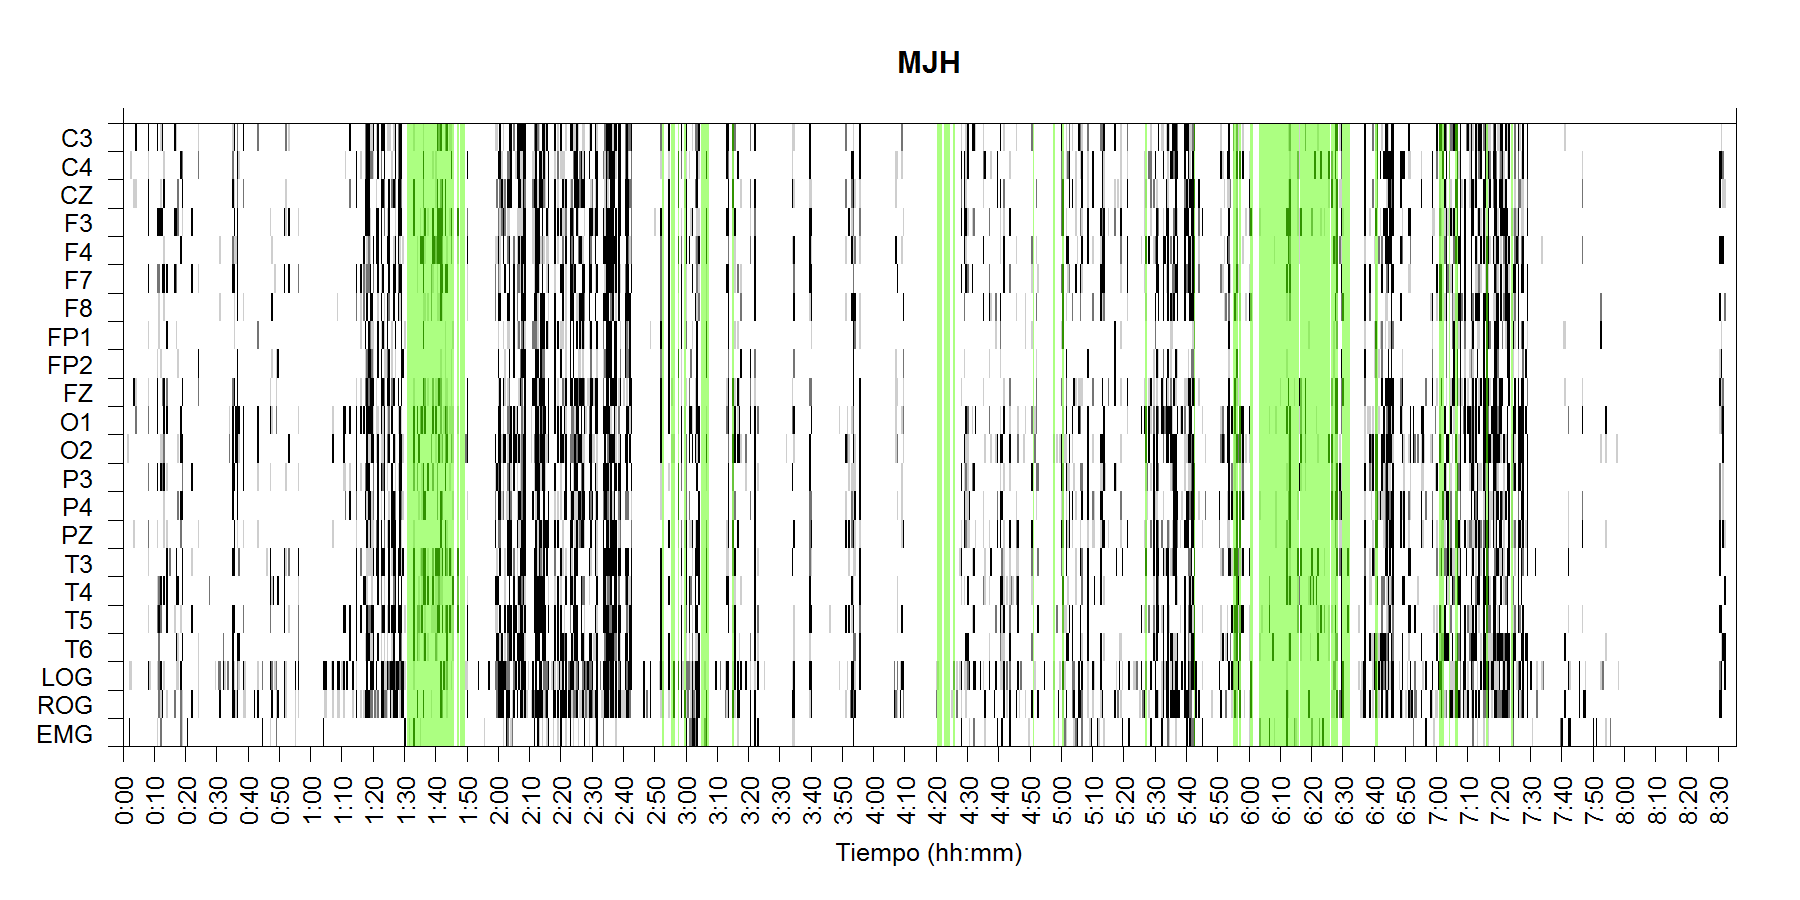
\includegraphics[width=0.9\linewidth]
{./g170413/MJNNVIGILOS_est.png} 
%\caption{Sujeto: MJH | Total \'epocas: 1032 | \'Epocas MOR: 127
%%| Frecuencia de muestreo: 200 Hz
%}
\label{grf_MJH}
\end{figure}

%%%%%%%%%%%%%%%%%%%%%%%%%%%%%%%%%%%%%%%%%%%%%%%%%

\begin{figure}
\centering
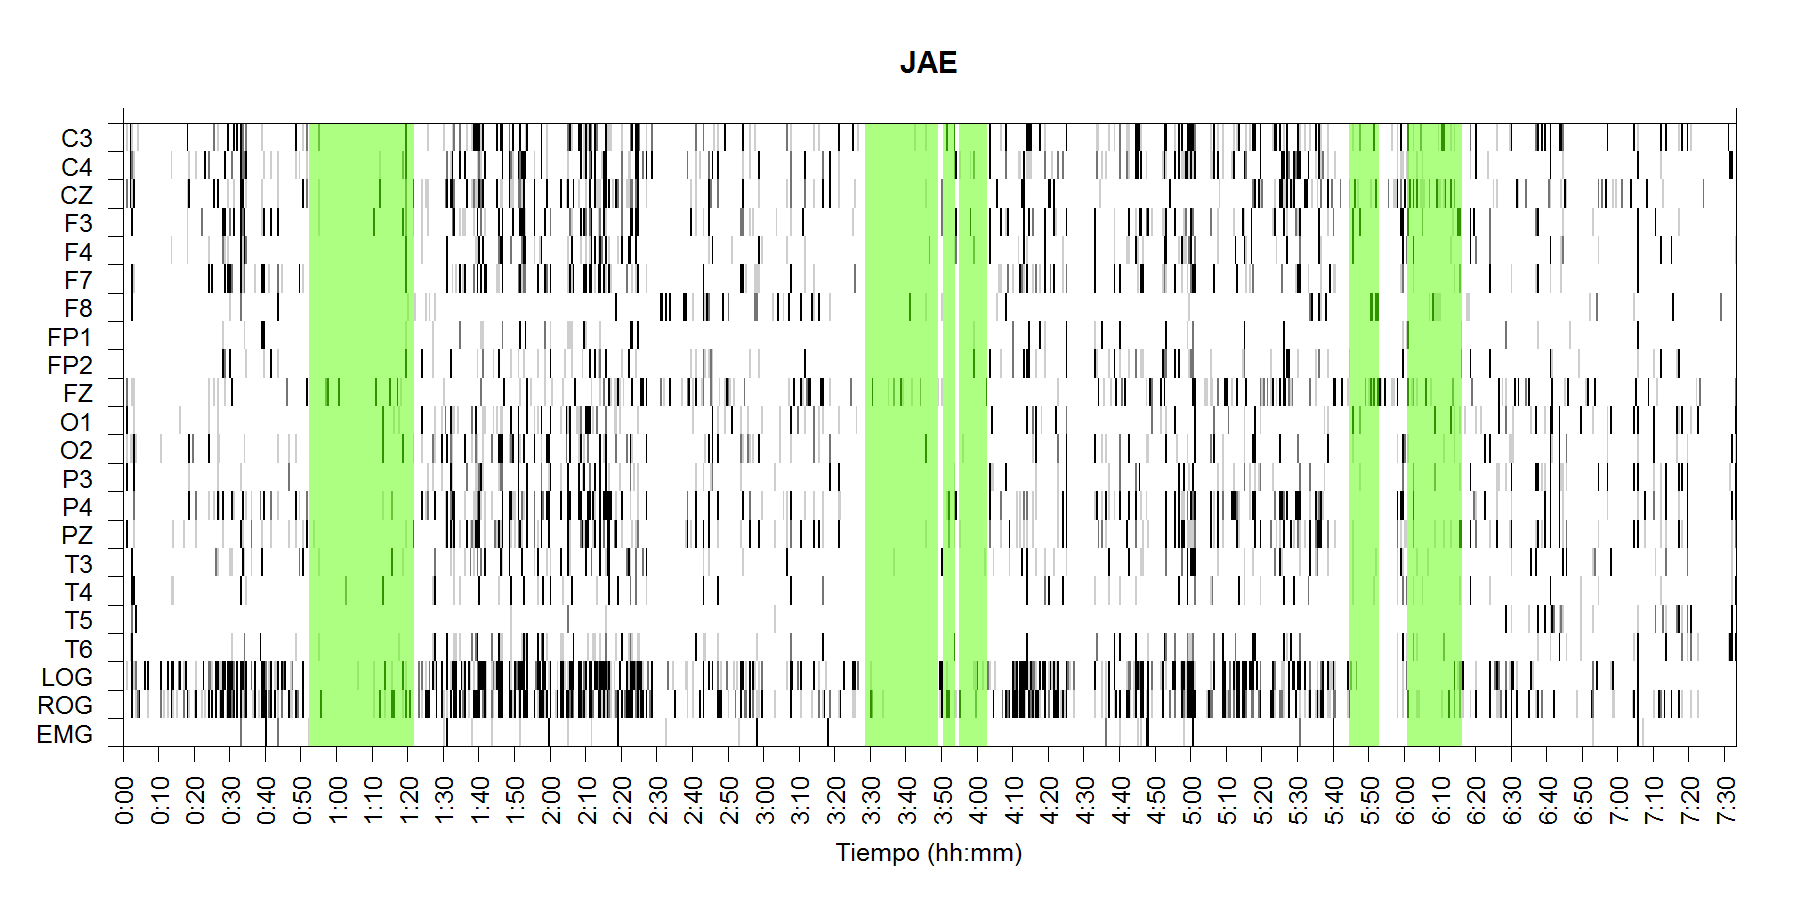
\includegraphics[width=0.9\linewidth]
{./g170413/JANASUE_est.png} 
%\caption{Sujeto: JAE | Total \'epocas: 907 | \'Epocas MOR: 171
%%| Frecuencia de muestreo: 200 Hz
%}
\label{grf_JAE}
\end{figure}

%%%%%%%%%%%%%%%%%%%%%%%%%%%%%%%%%%%%%%%%%%%%%%%%%

\begin{figure}
\centering
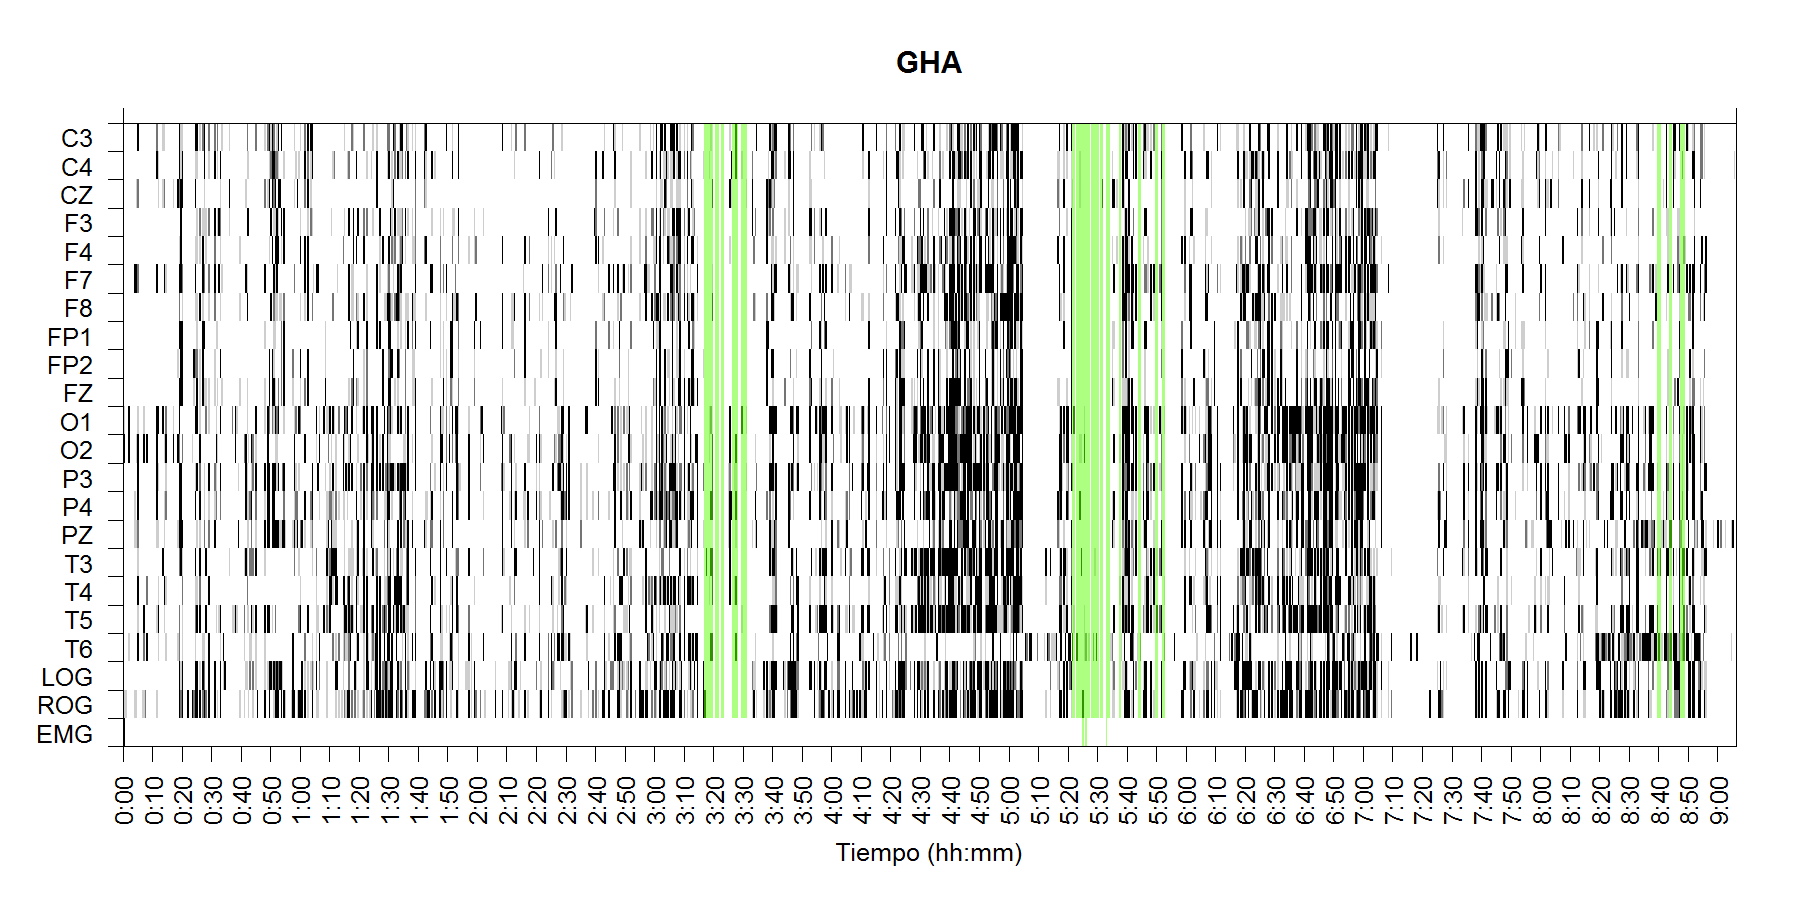
\includegraphics[width=0.9\linewidth]
{./g170413/GH24031950SUENNO_est.png} 
%\caption{Sujeto: GHA | Total \'epocas: 1093 | \'Epocas MOR: 55
%%| Frecuencia de muestreo: 200 Hz
%}
\label{grf_GHA}
\end{figure}

%%%%%%%%%%%%%%%%%%%%%%%%%%%%%%%%%%%%%%%%%%%%%%%%%

\begin{figure}
\centering
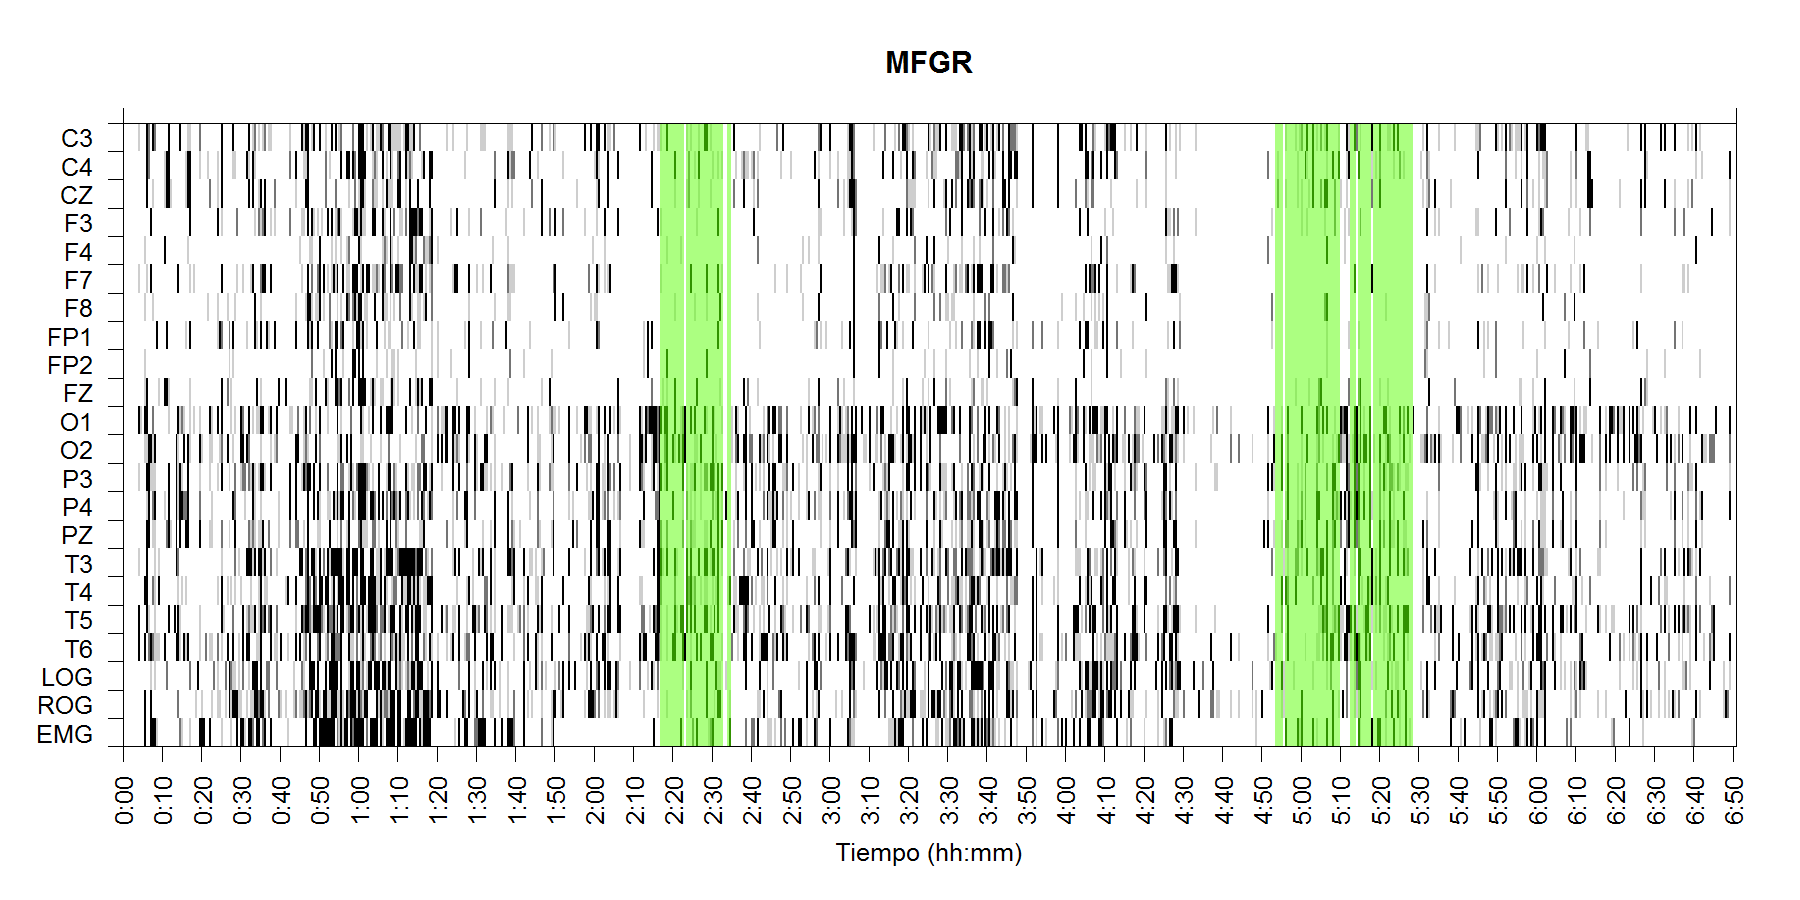
\includegraphics[width=0.9\linewidth]
{./g170413/GURM251148SUE_est.png} 
%\caption{Sujeto: MFGR | Total \'epocas: 822 | \'Epocas MOR: 95
%%| Frecuencia de muestreo: 200 Hz
%}
\label{grf_MFGR}
\end{figure}

%%%%%%%%%%%%%%%%%%%%%%%%%%%%%%%%%%%%%%%%%%%%%%%%%

\begin{figure}
\centering
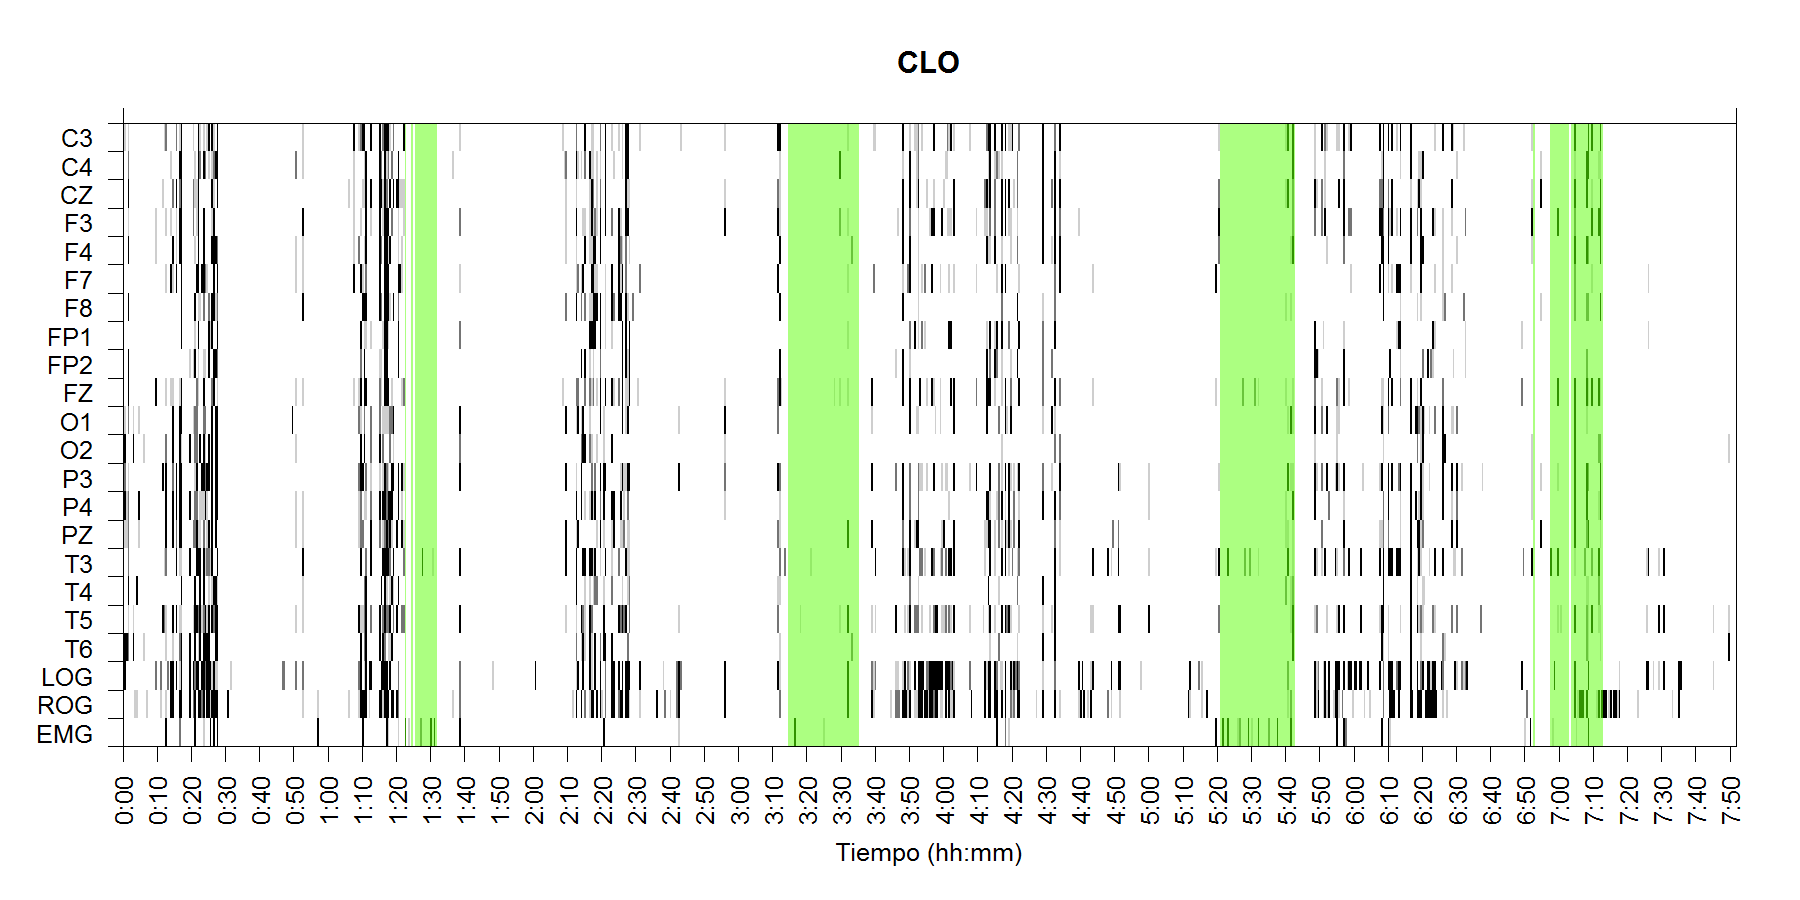
\includegraphics[width=0.9\linewidth]
{./g170413/CLMN10SUE_est.png} 
%\caption{Sujeto: CLO | Total \'epocas: 944 | \'Epocas MOR: 132
%%| Frecuencia de muestreo: 200 Hz
%}
\label{grf_CLO}
\end{figure}

%%%%%%%%%%%%%%%%%%%%%%%%%%%%%%%%%%%%%%%%%%%%%%%%%

\begin{figure}
\centering
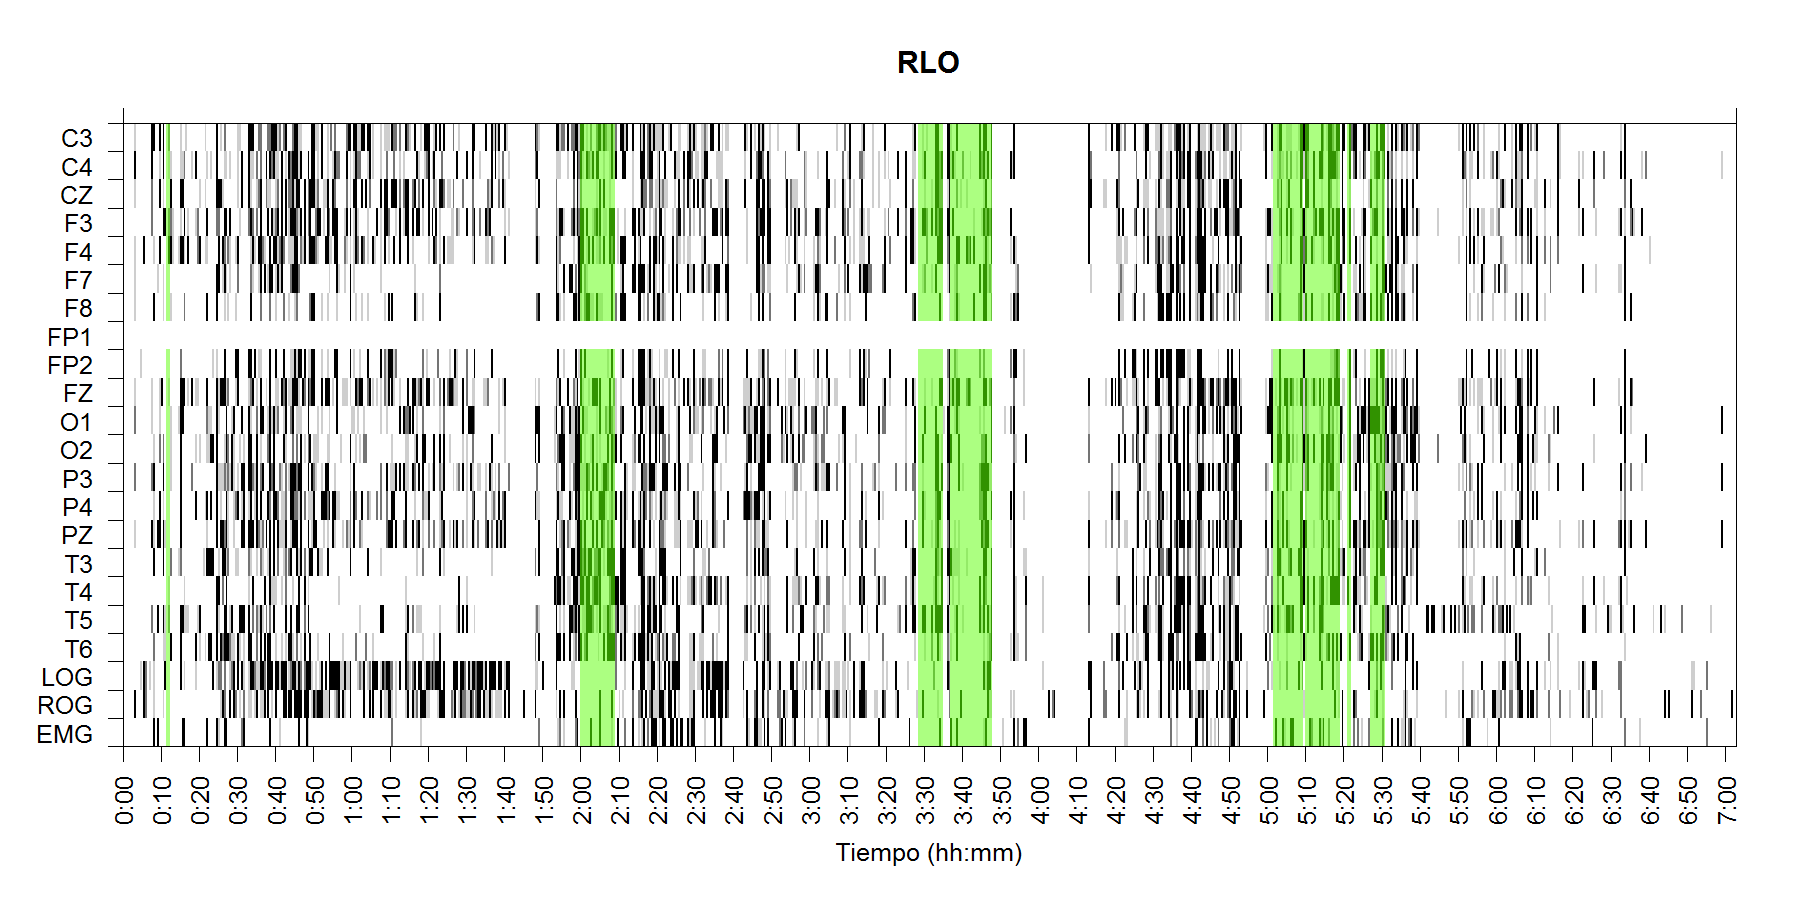
\includegraphics[width=0.9\linewidth]
{./g170413/RLMN10SUE_est.png} 
%\caption{Sujeto: RLO | Total \'epocas: 846 | \'Epocas MOR: 99
%%| Frecuencia de muestreo: 200 Hz
%}
\label{grf_RLO}
\end{figure}

%%%%%%%%%%%%%%%%%%%%%%%%%%%%%%%%%%%%%%%%%%%%%%%%%

\begin{figure}
\centering
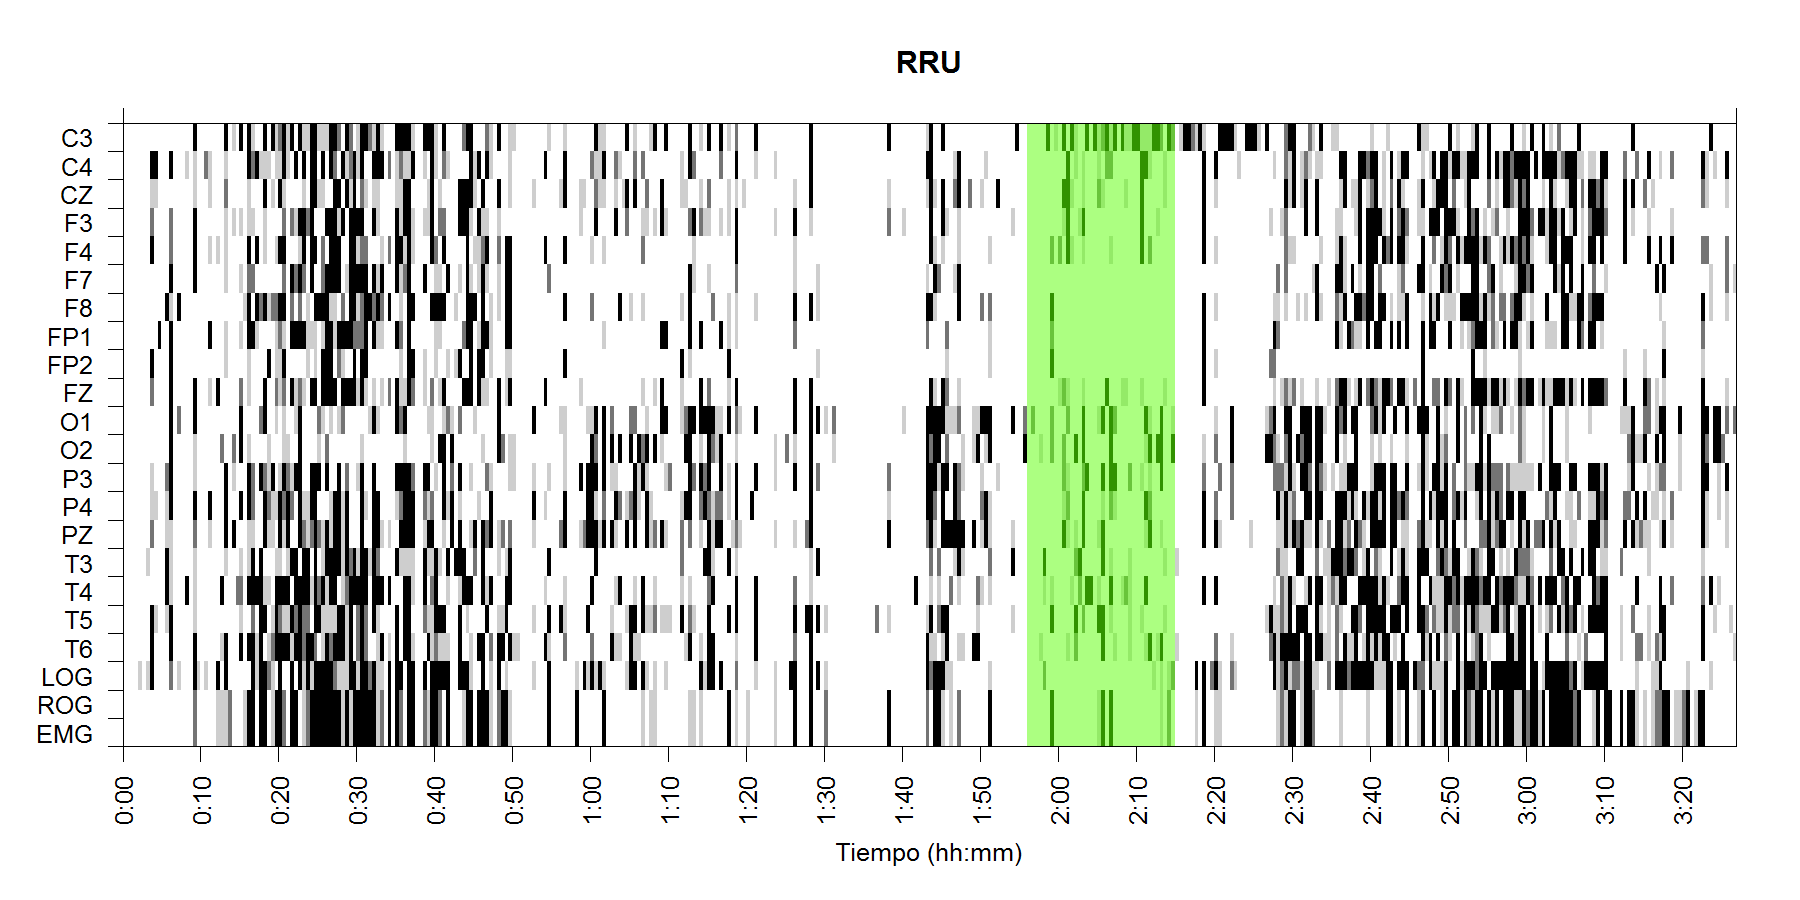
\includegraphics[width=0.9\linewidth]
{./g170413/RRMNS_est.png} 
%\caption{Sujeto: RRU | Total \'epocas: 414 | \'Epocas MOR: 38
%%| Frecuencia de muestreo: 200 Hz
%}
\label{grf_RRU}
\end{figure}

%%%%%%%%%%%%%%%%%%%%%%%%%%%%%%%%%%%%%%%%%%%%%%%%%

\begin{figure}
\centering
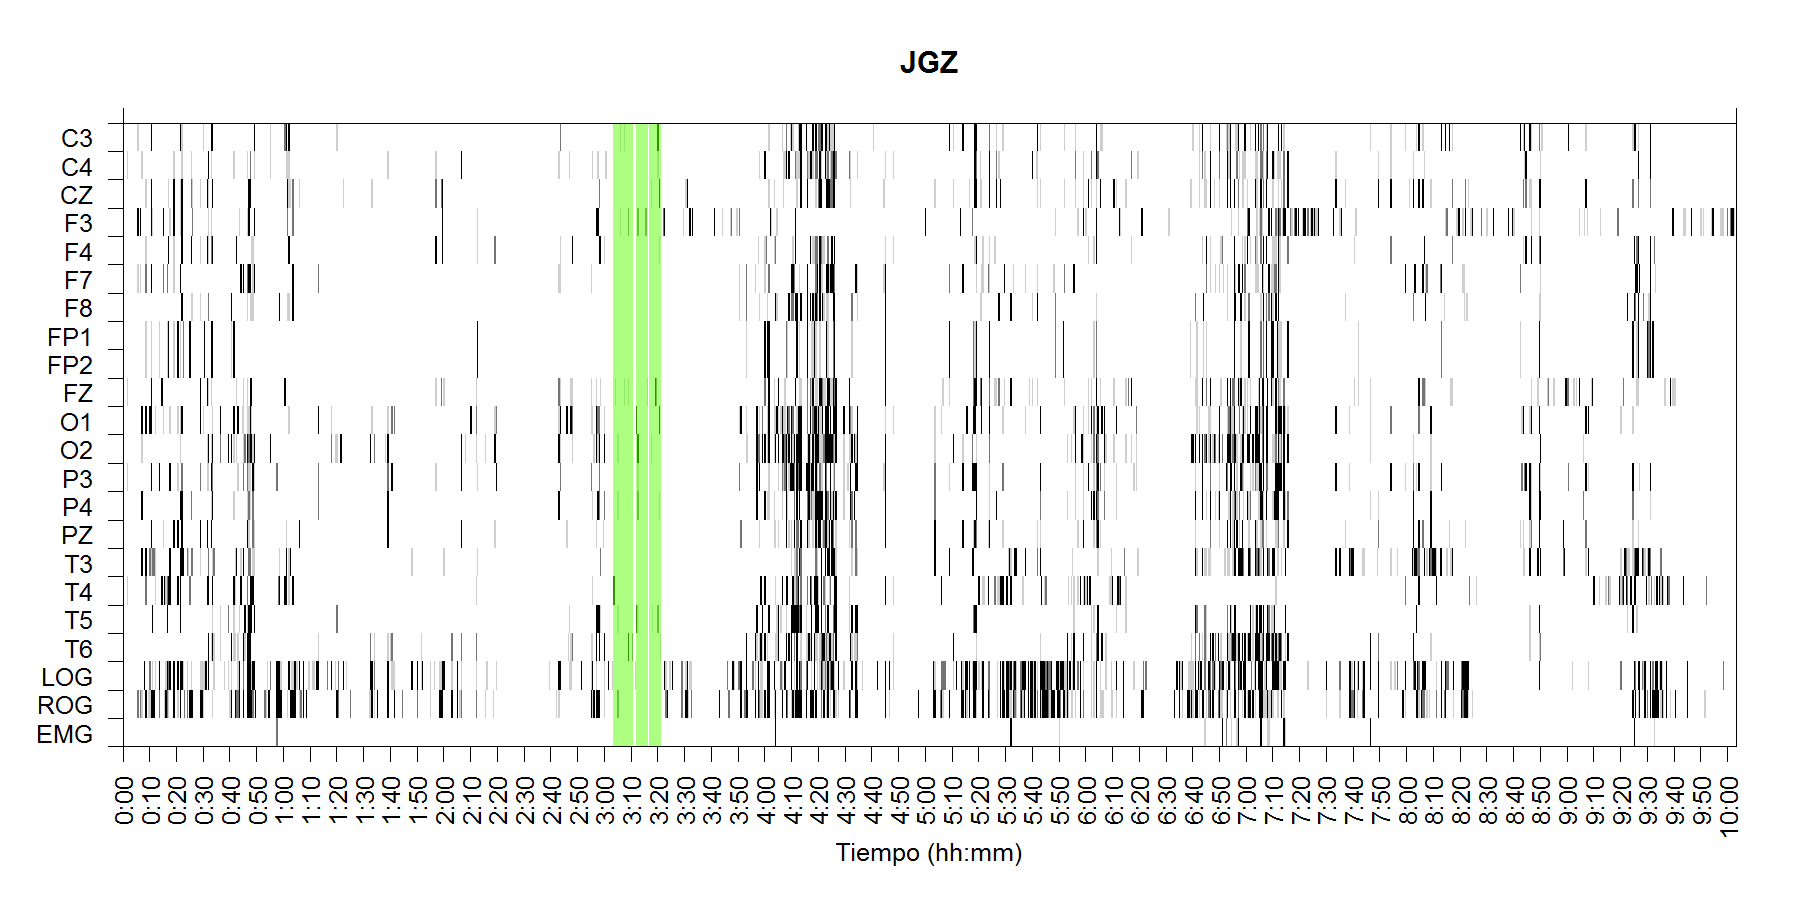
\includegraphics[width=0.9\linewidth]
{./g170413/JGMN6SUE_est.png} 
%\caption{Sujeto: JGZ | Total \'epocas: 1207 | \'Epocas MOR: 33
%%| Frecuencia de muestreo: 200 Hz
%}
\label{grf_JGZ}
\end{figure}

%%%%%%%%%%%%%%%%%%%%%%%%%%%%%%%%%%%%%%%%%%%%%%%%%

\begin{figure}
\centering
\includegraphics[width=0.9\linewidth]
{./g170413/FGHSUE_est.png} 
%\caption{Sujeto: FGH | Total \'epocas: 405 | \'Epocas MOR: 22
%%| Frecuencia de muestreo: 200 Hz
%}
\label{grf_FGH}
\end{figure}

%%%%%%%%%%%%%%%%%%%%%%%%%%%%%%%%%%%%%%%%%%%%%%%%%

\begin{figure}
\centering
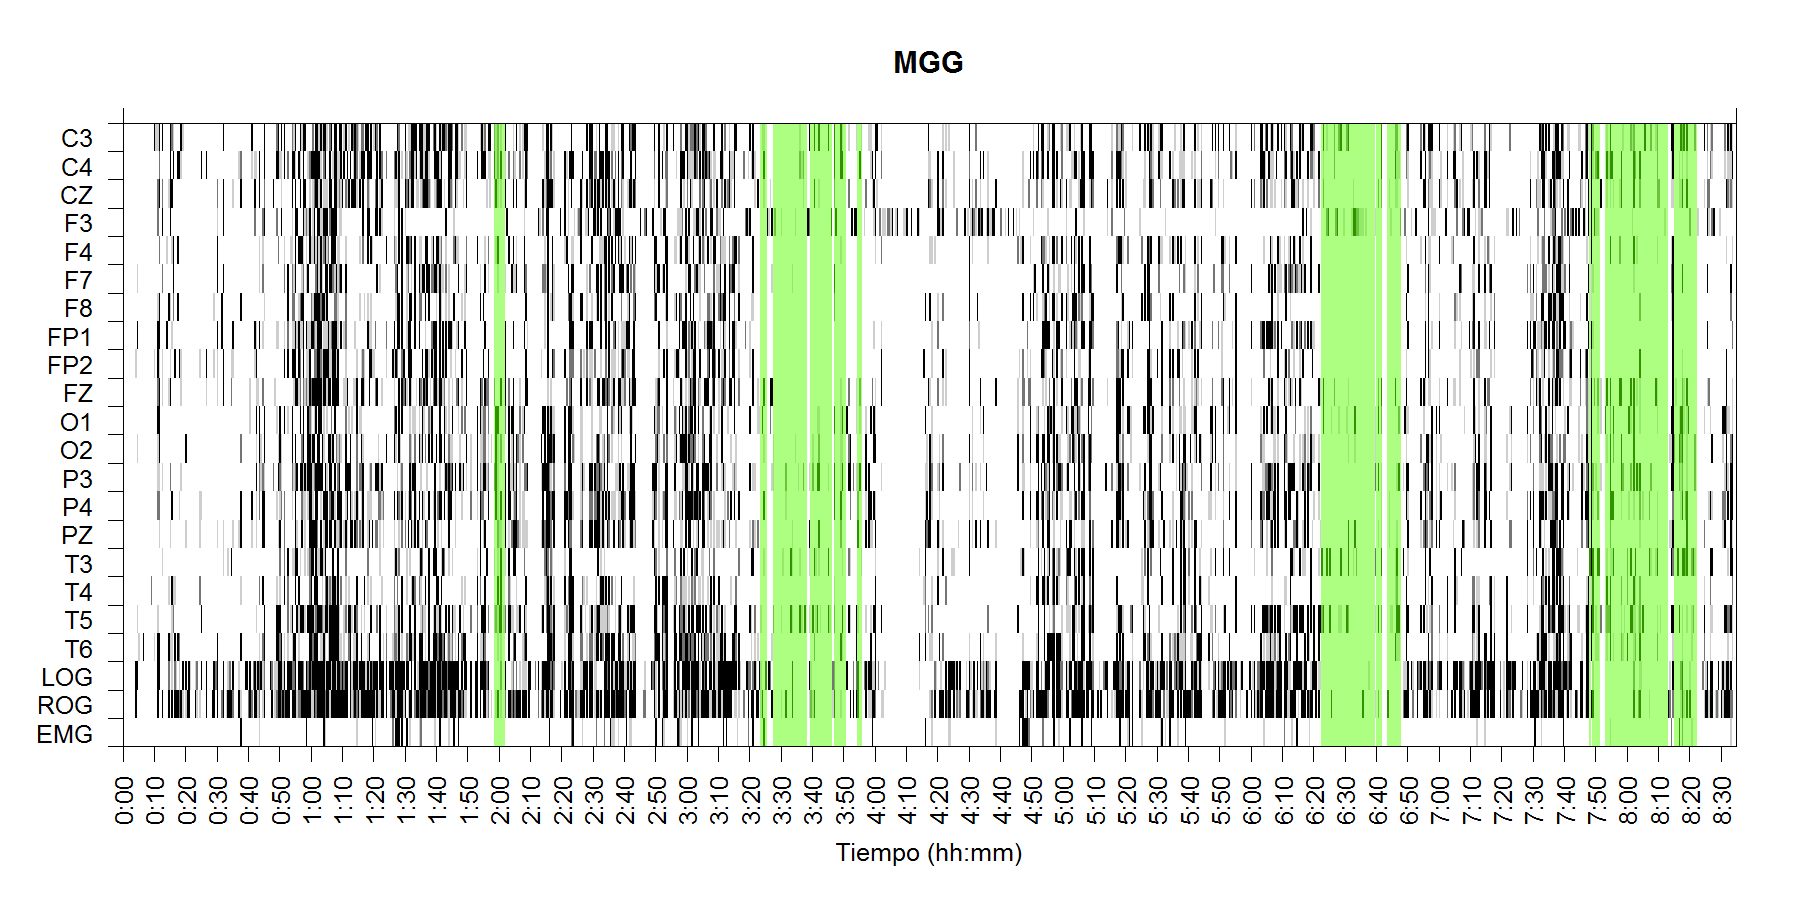
\includegraphics[width=0.9\linewidth]
{./g170413/MGNA5SUE_est.png} 
%\caption{Sujeto: MGG | Total \'epocas: 1030 | \'Epocas MOR: 166
%%| Frecuencia de muestreo: 200 Hz
%}
\label{grf_MGG}
\end{figure}

%%%%%%%%%%%%%%%%%%%%%%%%%%%%%%%%%%%%%%%%%%%%%%%%%

\begin{figure}
\centering
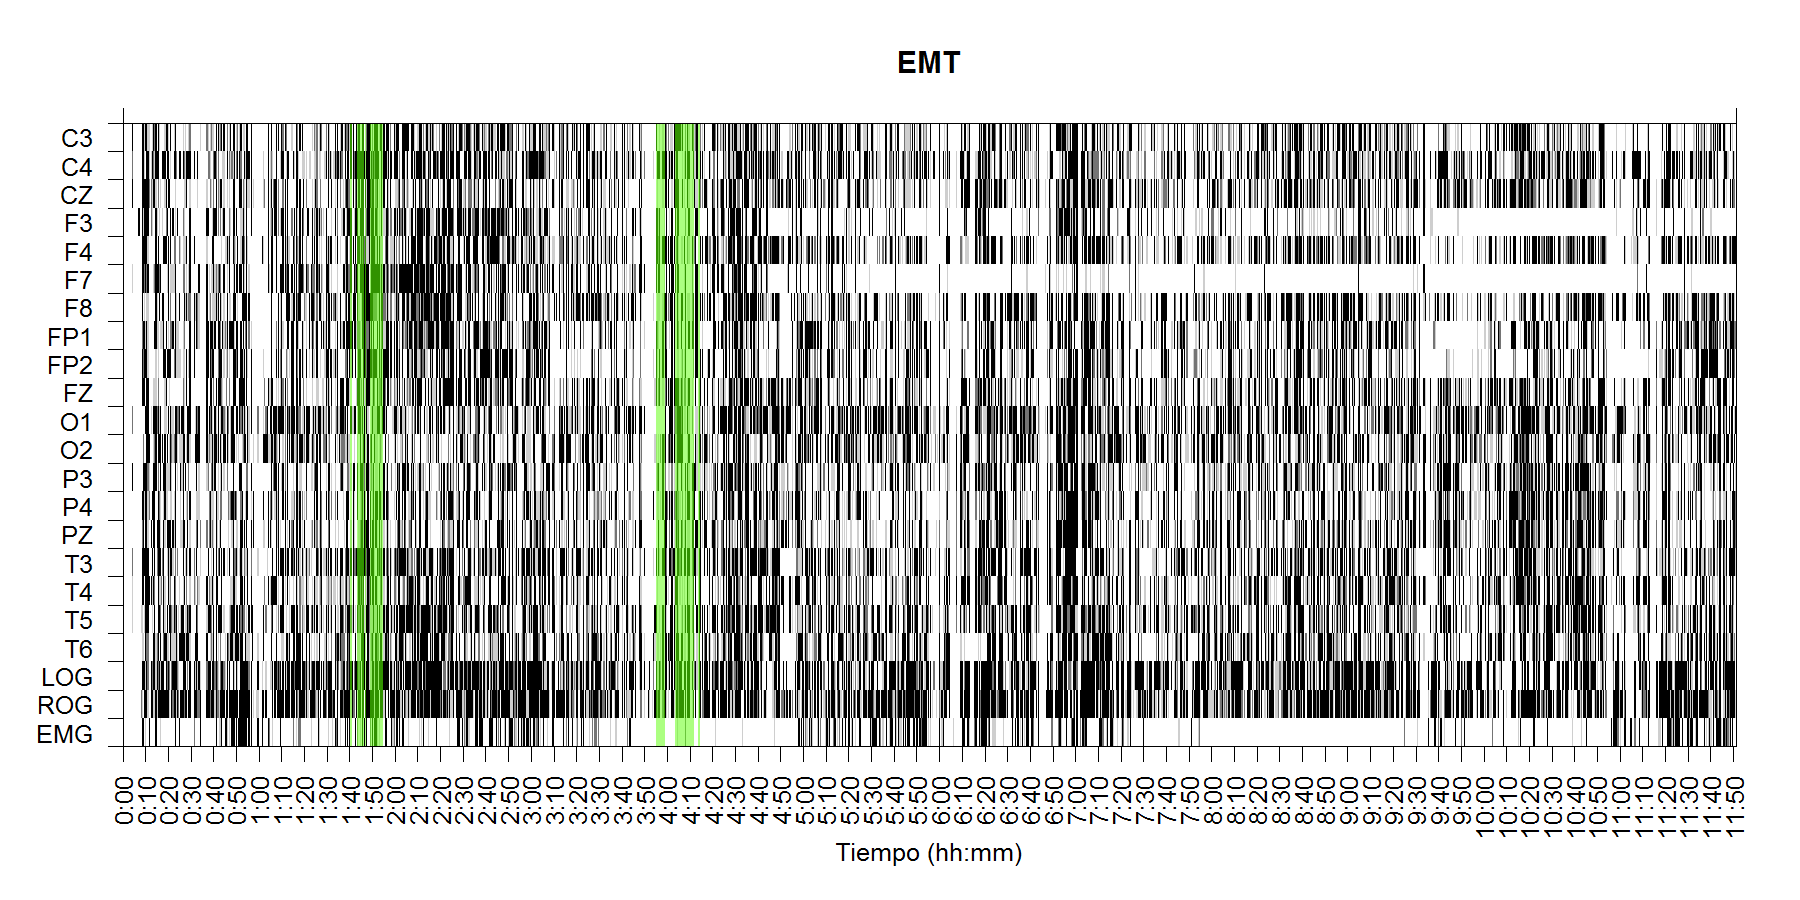
\includegraphics[width=0.9\linewidth]
{./g170413/EMNNS_est.png} 
%\caption{Sujeto: EMT | Total \'epocas: 1423 | \'Epocas MOR: 47
%%| Frecuencia de muestreo: 200 Hz
%}
\label{grf_EMT}
\end{figure}

%%%%%%%%%%%%%%%%%%%%%%%%%%%%%%%%%%%%
%%%%%%%%%%%%%%%%%%%%%%%%%%%%%%%%%%%%

%\begin{figure}
%\centering
%\includegraphics[width=0.9\linewidth]
%{./g170413/azul_VCR.png} 
%\label{azul_VCR}
%\end{figure}
%
%%%%%%%%%%%%%%%%%%%%%%%%%%%%%%%%%%%%%
%
%\begin{figure}
%\centering
%\includegraphics[width=0.9\linewidth]
%{./g170413/azul_MJH.png} 
%\label{azul_MJH}
%\end{figure}
%
%%%%%%%%%%%%%%%%%%%%%%%%%%%%%%%%%%%%%
%
%\begin{figure}
%\centering
%\includegraphics[width=0.9\linewidth]
%{./g170413/azul_JAE.png} 
%\label{azul_JAE}
%\end{figure}
%
%%%%%%%%%%%%%%%%%%%%%%%%%%%%%%%%%%%%%
%
%\begin{figure}
%\centering
%\includegraphics[width=0.9\linewidth]
%{./g170413/azul_GHA.png} 
%\label{azul_GHA}
%\end{figure}

%%%%%%%%%%%%%%%%%%%%%%%%%%%%%%%%%%%%%%%%%%%%%%%%%%%%%%%%%%%%%%%%%%%%%%%%%%%%%%%%%%%%%%%%%%%%%%%%%%%
%%%%%%%%%%%%%%%%%%%%%%%%%%%%%%%%%%%%%%%%%%%%%%%%%%%%%%%%%%%%%%%%%%%%%%%%%%%%%%%%%%%%%%%%%%%%%%%%%%%

%%%%%%%%%%%%%%%%%%%%%%%%%%%%%%%%%%%%%%%%%%%%%%%%%%%%%%%%%%%%%%%%%%%%%%%%%%%%%%%%%%%%%%%%%%%%%%%%%%%
%%%%%%%%%%%%%%%%%%%%%%%%%%%%%%%%%%%%%%%%%%%%%%%%%%%%%%%%%%%%%%%%%%%%%%%%%%%%%%%%%%%%%%%%%%%%%%%%%%%

%\phantomsection
%
%\addcontentsline{toc}{chapter*}{Bibliograf\'ia}

\bibliography{referencias_estacionariedad,referencias_fisiologia,referencias_otros,referencias_mixto}{}
%\bibliographystyle{apalike-es}
\bibliographystyle{abbrv}

%%%%%%%%%%%%%%%%%%%%%%%%%%%%%%%%%%%%%%%%%%%%%%%%%%%%%%%%%%%%%%%%%%%%%%%%%%%%%%%%%%%%%%%%%%%%%%%%%%%
%%%%%%%%%%%%%%%%%%%%%%%%%%%%%%%%%%%%%%%%%%%%%%%%%%%%%%%%%%%%%%%%%%%%%%%%%%%%%%%%%%%%%%%%%%%%%%%%%%%

\end{document}

%%%%%%%%%%%%%%%%%%%%%%%%%%%%%%%%%%%%%%%%%%%%%%%%%%%%%%%%%%%%%%%%%%%%%%%%%%%%%%%%%%%%%%%%%%%%%%%%%%%